\documentclass[11pt]{article}
\usepackage[T1]{fontenc}
\usepackage[margin=1in]{geometry}
\usepackage{amsmath,amssymb,amsthm,microtype,booktabs,array,longtable}
\usepackage[hidelinks]{hyperref}
\usepackage{xurl}
\usepackage{tikz}
\usetikzlibrary{arrows.meta,positioning}
\definecolor{sourceblue}{RGB}{29,83,135}
\definecolor{fliporange}{RGB}{166,76,0}
\definecolor{softblue}{RGB}{237,244,250}
\definecolor{softorange}{RGB}{255,244,232}
\usepackage{listings}
\lstset{basicstyle=\ttfamily\footnotesize,breaklines=true,columns=fullflexible,keepspaces=true,showstringspaces=false}
\newtheorem{lemma}{Lemma}
\newtheorem{theorem}{Theorem}
\newtheorem{proposition}[theorem]{Proposition}
\newtheorem{corollary}[theorem]{Corollary}
\newcommand{\G}{\mathsf{G}}\newcommand{\F}{\mathsf{F}}
\newcommand{\CPre}{\operatorname{CPre}}\newcommand{\Pref}{\operatorname{Pref}}
\newcommand{\EPre}{\operatorname{EPre}}\newcommand{\code}[1]{\texttt{#1}}
\newcolumntype{L}[1]{>{\raggedright\arraybackslash}p{#1}}
\title{Technical Appendix:\\
Auditing Controller Replacement after Environment-Model Change}
\author{Anonymous authors}
\date{}
\begin{document}
\maketitle
\section*{Reader guide to the main argument}
The main paper audits candidate exclusion in replacement planning.
Its Fig.~1 distinguishes source strict and source-kind questions, encoded
strict winning, public action and fixed raw solver calls.
The main argument proceeds from the basic strict theorem and corollary
proofs to Patrol's positive/negative argument, then the retained-duty
proposition with its full proof and application to the actual export.
Source-kind, case evidence and the conditioned cohort follow, before the
exclusion contract and three saved-evidence checks. Use this supplement to inspect
individual obligations; historical section labels remain stable.
\begin{center}\small
\begin{tabular}{@{}L{35mm}L{115mm}@{}}\toprule
I want to check\ldots & Start here\\\midrule
The preservation theorem & L.6 gives the complete relations, game-based definition of $W_C$, theorem/corollary proofs and corrected-guard proof. L.1 gives the retained-duty extension, its safety fixed point and example with two source states, also summarized after the main paper's complete proposition proof.\\[4pt]
The Patrol continuation & S and U.1 give the exact source/rules, positive witness and export binding; AB.6 gives the route. U.6 gives the reduced calculation. AD.4--AD.6 give the same-entry all-history completion; U.5/U.8 retain full-helper UNKNOWNs.\\[4pt]
The implementation comparisons & Vehicle: E/X and AD.3 for source proof, regions, initial quantifiers and target-specific Kind witnesses. Obstacle: AC.1--AC.4 for strict regions, AC.5--AC.7 for positive witnesses/public controls, AE for path scope, AG for the completed raw pair and AF for its distinct history.\\[4pt]
The reader tasks & \href{https://github.com/research-artifact-archive/seams2027/blob/controller-replacement-audit-20261026-v3/results/guides/VEHICLE188_WHOLE_REGION_EVIDENCE.md}{Vehicle guide}: saved loss membership and target predecessors. \href{https://github.com/research-artifact-archive/seams2027/blob/controller-replacement-audit-20261026-v3/results/guides/CONTINUATION_EVIDENCE.md}{Patrol guide}: positive policy, all-response countercertificate and typed export premises. Obstacle \href{https://github.com/research-artifact-archive/seams2027/blob/controller-replacement-audit-20261026-v3/results/guides/V71_R6_POSITIVE_CERTIFICATES_AND_CONTROLS.md}{source} and \href{https://github.com/research-artifact-archive/seams2027/blob/controller-replacement-audit-20261026-v3/results/guides/COMPLETED_SAME_OBSERVER_PAIR.md}{completed-pair guides}: source certificate, exact query, sole typed $0\to1$ SYS release and false/true records (AC.7, AG).\\\bottomrule
\end{tabular}
\end{center}
These guides refer to the accompanying release~\cite{artifactrepository};
its \href{https://github.com/research-artifact-archive/seams2027/blob/controller-replacement-audit-20261026-v3/paper/README.md}{paper reading map}
identifies the matching main paper, supplement and document source ZIP.
The tasks check saved evidence within each guide's stated scope; document
compilation does not rerun scientific computations.

\paragraph{Definitions retained in the technical sections.}
The main paper now defines $W_C$ directly through one source strict-winning
strategy that maintains $C$ at every induced source-legal finite prefix,
including the initial state, with its evolving memory. Section~L.6 retains
the equivalent $C\cap\operatorname{Win}_{\mathrm{str}}(M_C)$ formulation:
$M_C$ adds $C$ at both ends of each legal transition, while the outer $C$
covers the length-zero prefix and excludes outside-$C$ vacuous dead-end
winners. Replacing $C$ by $F$ gives the corresponding $W_F$ definition.
The initial-query quantifiers are in L.6; the all-history Kind quantifiers
and sufficient source-witness constructions are in AC.5 and AD.1--AD.3.
AD.2 also retains the general fair-ENV-selector lemma and full proof moved
from the main paper.
The main summarizes Patrol's all-history completion and Vehicle's per-target
reachability; their full constructions remain in AD.4--AD.6 and X/AD.3.
AC.7 gives the phase/rank certificate obligations now summarized for Obstacle B.

For statewise strict queries over $D_{\rm query}\subseteq D$, preserving
each queried source winner requires
$W\cap D_{\rm query}\subseteq W_R(\cdot,0)$.
The right side is $W_C$ or $W_F$ under the applicable hypotheses; a
strategy may leave $D_{\rm query}$ and must continue to maintain its response
option. Initialized strict synthesis instead requires equality of the Boolean
decisions $I_M(W)$ and $I_M(W_R(\cdot,0))$, with unchanged initializers and
initial $b=0$. Section~L.6 defines $I_M$ by $\forall$ENV$\exists$SYS:
for an initially realizable source, each allowed ENV initial value needs
at least one allowed surviving SYS response. Preservation of every winning
initial response, or of the whole source-winning region, is sufficient
but not generally necessary. A sound negative oracle also needs the stated
query/objective correspondence. This is a reasoning contract, not an
implemented online gate.

\paragraph{Unfavorable results and history.}
J and AB.4--AB.5 retain the stopped 59-model selection, outcomes and shared
dependencies; Y and AA retain separate controlled comparisons. K and the
archive directory below locate saved records and their checking scope.
All historical UNKNOWNs remain. A and L.2 preserve the earlier normalized
cooperative derivation; those results are not prerequisites silently added
to the main strict-preservation theorem.



\paragraph{Release and archive scope.}
This supplement supplies proofs, exact source bindings, saved proof
objects and bounded software studies. The accompanying document and evidence release is
\href{https://github.com/research-artifact-archive/seams2027/tree/controller-replacement-audit-20261026-v6}{\nolinkurl{controller-replacement-audit-20261026-v6}}.
Its \href{https://github.com/research-artifact-archive/seams2027/blob/controller-replacement-audit-20261026-v6/paper/README.md}{paper reading map}
identifies the matching PDFs and document source ZIP, which rebuilds the
documents without rerunning scientific computations. AF and AG identify
separate experimental archives and their checking scope; those archives
are not part of the document source ZIP.

The repository's \path{paper/}, \path{results/}, \path{tool/},
\path{reproduce/} and \path{docs/} directories organize the paper,
evidence, code, scoped checks and version guidance. Bundles are in
\path{results/archives/}, with guides in \path{results/guides/}.
The five added packages below preserve earlier scientific results and
UNKNOWNs; the fifth adds the positive source certificates and matched
ordinary-mode controls in AC.7. The existing continuation release contains selected Patrol,
manager, reduced-query and fixed-lasso records; it does not distribute
the complete local Section~U archive. The full contract-contrast,
equivalent-old-source and U.4 runtime records retain their local scope.
Section~K retains the historical archive map.

Fixed-version paths below are relative to
\url{https://github.com/research-artifact-archive/seams2027} at their stated
immutable tags. Earlier evidence tags and layouts remain unchanged.
Archive names are literal; fresh output directories must be new or
empty as each entrypoint requires.

\paragraph{Archive starting points.}
Patrol's continuation release contains saved semantic replay for the
Patrol, reduced-query, manager and fixed-lasso records (U--V), without new
native execution. The separate Vehicle188 package supplies saved full-region
membership and initialization checks (E), without a native solver rerun.
Entry~1 supplies saved source and arena checks for Guard and certificates
(L, N, P--Q); certificate revalidation is separate from new synthesis.
Entry~2 supplies saved Lift graph replay and a separate kit that regenerates
one matched pair (H, K). Entry~3 rechecks 76 saved files and exact external
sources for earlier Patrol and extended Lift (S, R.7), without a controller
or native solver rerun.

\subsection*{Added packages: cohorts, Obstacle and historical bindings}
In the accompanying release, the five archive paths below are relative to
\path{results/archives/}. Their package identifiers are distinct from
supplement section labels. Each guide gives entry points and the scope
of checking; a static integrity check is not a scientific replay.
\begin{center}\small
\begin{tabular}{@{}L{24mm}L{73mm}L{53mm}@{}}\toprule
Package & Archive & Guide in \path{results/guides/}\\\midrule
AA: 44-arm cohort & \path{v71-compiled-cohort-evidence-20261026.zip} & \path{V71_COMPILED_COHORT.md}\\[3pt]
AC: Obstacle & \path{v71-obstacle-evidence-20261026.zip} & \path{V71_OBSTACLE_CERTIFICATES.md}\\[3pt]
Z: historical Patrol & \path{v71-historical-patrol-source-20261026.zip} & \path{V71_HISTORICAL_PATROL.md}\\[3pt]
AD: public Kind & \path{v71-public-kind-gui-evidence-20261026.zip} & \path{V71_PUBLIC_KIND_GUI.md}\\[3pt]
R6: positive / control & \path{v71-r6-positive-certificates-and-controls-20261026.zip} & \path{V71_R6_POSITIVE_CERTIFICATES_AND_CONTROLS.md}\\\bottomrule
\end{tabular}
\end{center}

\paragraph{Compiled variants (Section~AA).}
Extract \path{aa_compiled44/}; start with \path{README.txt} and
\path{COHORT_INDEX.json}. The conditioned eleven-source roster has 44
arms: 43 saved native candidates, 40 accepted results and four UNKNOWNs.
\path{SOURCE_RESTORATION.json} binds the required primitives and shared
checkers to exact members of the unchanged Core and FixedSevenNative
archives. The \path{replay_saved.py} adapter for the 40 accepted arms is
unexecuted after relocation and has no external wall/RSS supervisor;
it excludes the four UNKNOWNs. Packaging adds no fresh-host replay.

\paragraph{Obstacle certificates and reached states (Section~AC).}
Extract \path{ac_obstacle8cert98/}; start with \path{README.txt} and
\path{published_update/direct_certificate_check/amendment_01/FINAL_CERTIFICATE_SUMMARY.json},
\path{FINAL_CERTIFICATE_TABLE.csv}, and \path{ALL98_FIXED8_MEMBERSHIP.json}
in that directory. Eight accepted theorem-based certificates preserve
the fixed order of all 98 boundary states. The earlier eight independent
exported-game fixed-point attempts remain UNKNOWN: two source and six
helper arms. The separate initial certificate protocol retains one
serialization UNKNOWN and seven unattempted cases. Later certificates
do not relabel those attempts. \path{SOURCE_RESTORATION.json} and
\path{restore_sources.py} provide a hash-bound local recipe for omitted
distributor specifications and the ordinary projection. Neither
restoration nor relocated certificate replay was performed for publication.

\paragraph{Two public Kind observations (Section~AC.6).}
Extract \path{ad_gui_kind_ab/}; start with \path{SCIENTIFIC_DISPOSITION.json},
\path{gui/A/RESULT.json}, \path{gui/B/RESULT.json}, and the associated
\path{COMPLETION_AUDIT_PUBLIC.json} records. A is the unchanged old
authored-initial query; B fixes the updated point $r2404$. Each public
action returned false once. The source-kind bridge is retained in
\path{theory/SOURCE_KIND_LEMMA.txt} and its adoption record. The preparation
exporter's supervisor remains UNKNOWN with an unrecorded OS exit code;
the later saved-predicate gate is separate. Raw screenshots and AX captures
are omitted; authored observations, exact logger XML and source-snapshot
hashes are retained. A manual console transcription is not raw process output.

\paragraph{Positive witnesses and ordinary-mode controls (Section~AC.7).}
Extract \path{r6_positive_certificates_and_controls/}; start with
\path{SCIENTIFIC_DISPOSITION.json} and the fifth guide above.
\path{certificates/A.json}, \path{certificates/B.json},
\path{checkers/check_certificate.py} and
\path{theory/INDEPENDENT_CHECKER_RATIONALE.md} supply the direct-source
positive witnesses and their checker. Acceptance and separate
ENV-totality receipts are under \path{c1/stages/}; qualification records
are in \path{c1/stages/checker_qualification/qualification/}.
These positive witnesses are distinct from AC.4's saved-region/theorem
certificates; the earlier eight full-fixed-point UNKNOWNs remain.

\path{c2/A/RESULT.json} and \path{c2/B/RESULT.json} record ordinary-GR(1)
true answers, one action each; \path{prior_kind/A/RESULT.json} and
\path{prior_kind/B/RESULT.json} retain the previous selected Kind false
answers. Console transcriptions and logger XML accompany the records.
\path{SOURCE_RESTORATION.json} binds the five exact input files through
distributor/member hashes and documented projection/initializer changes.
Upstream source bodies, archived source bodies, raw screenshots and AX
captures are omitted from public redistribution. An authored visual
console transcription is not raw stdout. The guide specifies the
package's validation scope; no fresh-host scientific replay is inferred
from these authoring records.

For the joint static check of the four earlier packages only, extract them
into one fresh parent directory, retaining \path{aa_compiled44/}, \path{ac_obstacle8cert98/},
\path{z_historical_patrol/}, and \path{ad_gui_kind_ab/}. Then run:
\begin{verbatim}
cd /path/to/fresh-parent/ad_gui_kind_ab
python3 -I -S -B verify_candidate.py
\end{verbatim}
This checks the adjacent AC scientific files and all three sibling
assembly manifests. The unexecuted saved-predicate adapter requires AC
scientific inputs only; that smaller dependency set is insufficient for
the complete static verifier. No new GUI action or synthesis occurs.

\paragraph{Historical Patrol (Section~Z).}
Extract \path{z_historical_patrol/}; read \path{README.txt},
\path{historical/ORIGINAL_ARTIFACT_PATROL_EVIDENCE.json} and
\path{historical/AUDIT.json}. The archived report records
\code{1670358790.spectra,TRUE,FALSE} for \code{Filename,4FP,R+4FP}.
Here R+4FP means reduction plus four fixed points, not this paper's
preserving $R^+$ construction. The package binds that historical report
and its source; it adds no artifact execution or current-default/GUI
equivalence. Third-party source text and runtime binaries are omitted;
\path{SOURCE_RESTORATION.json} gives exact distributor/member pins.

\subsection*{Existing continuation release: selected evidence}
Use \href{https://github.com/research-artifact-archive/seams2027/blob/continuation-evidence-20261024-v1/CONTINUATION_EVIDENCE.md}{\nolinkurl{continuation-evidence-20261024-v1}}~\cite{continuationartifact}.
The guide identifies \path{archives/continuation-evidence-20261024-v1.zip};
inside it start with \path{REVIEWER_START_HERE.txt} and
\path{claim_to_evidence.json}. The 41 original records retain their exact
bytes and source-member ledger. \path{quick_verify.py} checks transport
identity and recorded properties only; its PASS is not semantic replay.

For the saved Patrol, sequential-manager, and reduced-query checks, use:
\begin{verbatim}
python3 -B "$BUNDLE_ROOT/replay/replay.py" \
  --bundle "$BUNDLE_ROOT/replay" --out "$FRESH_REPLAY"
\end{verbatim}
Here \code{BUNDLE\_ROOT} is the absolute extracted archive root and
\code{FRESH\_REPLAY} is a new or empty external output directory.
Python~3.9+ and the standard library suffice; optimized Python is rejected.
Expected result: \code{PASS\_PORTABLE\_SAVED\_EVIDENCE}, with stages
\code{patrol}, \code{manager}, and \code{reduced}. The reduced stage binds
the saved winning output and all 4,800 layout memberships; it does not
recompute the native winning fixed point. No native synthesis, extraction,
manager-worker execution, or full-helper retry occurs; full-helper UNKNOWN
is unchanged. Historical source/runtime and worker-provenance checks omitted
from replay are listed in \path{replay/OMITTED_HISTORICAL_CHECKS.json}.
Qualification is an author-host fresh-directory sandbox check with workspace
and network access denied, not an external reproduction.

For the separately qualified fixed lasso in Section~V, use:
\begin{verbatim}
python3 -I -S -B \
  "$BUNDLE_ROOT/lasso/replay/replay_lasso.py" \
  --bundle "$BUNDLE_ROOT/lasso/replay" \
  --out "$FRESH_LASSO_OUTPUT" --timeout-seconds 60
\end{verbatim}
This Python~3.10+/POSIX standard-library check expects
\code{PASS\_SAVED\_LASSO\_REPLAY}. It checks 23 public semantic payloads,
nine metadata projection values and 19 DAGs, not the original 25-pin local
verification. Original Spectra and \path{final_region} are hash-only
omitted; source-value equality is assembly-time evidence and original
paths/runtime provenance are not revalidated. It evaluates one fixed
initialized transformed-arena lasso, not a returned controller.

Older Guard and matched-Lift kits remain separate; use
\path{REPLAY_COMMANDS.txt} and Entries~1--2 for their restoration steps and
qualification boundaries. The full local R5 archive is not distributed.

\subsection*{Separate evidence: Vehicle188 native strict pair}
The separately packaged Vehicle188 records are identified by
\href{https://github.com/research-artifact-archive/seams2027/blob/vehicle188-native-evidence-20261024-v1/VEHICLE188_NATIVE_EVIDENCE.md}{\nolinkurl{vehicle188-native-evidence-20261024-v1}}~\cite{vehicleartifact}.
Inside the bundle, start with \path{README.txt}, \path{MANIFEST.json},
\path{TRANSFORMATIONS.json}, and \path{OMITTED_HISTORICAL_CHECKS.json}.
For a saved-evidence check using Python~3.10+ and its standard library:
\begin{verbatim}
python3 -I -S -B "$BUNDLE_ROOT/replay.py" \
  --bundle "$BUNDLE_ROOT" --out "$FRESH_RESULT_JSON"
\end{verbatim}
The result file must be new and outside the immutable bundle. Expected status:
\begin{verbatim}
PASS_SAVED_IDENTITY_MEMBERSHIP_INITIALIZATION
\end{verbatim}
The check verifies transport integrity, exact saved model/function identity,
the full fixed source state and helper-false target, saved winning-region
membership/counts, and quantified initialization. It does not recompute a
winning fixed point, run a native solver, or replay the separate source-policy
certificate. Historical complete-memory, process and loaded-class checks
remain recorded evidence. The native experiment itself is described in
Section~E; its two calls are distinct from this saved-data check.
The bundle preserves encoded stdout, with no raw-stream hash claim.
Local qualification uses an isolated directory with workspace and network
access denied, including positive and corrupted-input checks; it does not
establish external reproduction.

\subsection*{1. Guard, source certificates, and finite studies}
Use tag
\href{https://github.com/research-artifact-archive/seams2027/tree/certificate-finite-evidence-20261023-v2}{\nolinkurl{certificate-finite-evidence-20261023-v2}}~\cite{newartifact}
and its \path{CERTIFICATE_FINITE_EVIDENCE.md}. The two downloads are
\path{archives/three-study-evidence-20261023-v2.zip} and
\path{archives/intruder-certificate-evidence-20261023-v1.zip}.
From that repository version, Python~3.10+ and its standard library suffice
for the following \emph{integrity-only} check:
\begin{lstlisting}
python3 -I -S -B tools/verify_current_distribution.py
\end{lstlisting}
It checks the version's 302-file distribution and 22 downloads, not any
scientific result. Do not substitute the older version-bound certificate
verifier for this v2 metadata check.

\paragraph{Guard and the finite-study tree.}
After extracting the three-study archive, set \texttt{BUNDLE} to its
\path{three-study-evidence-20261023-v2/saved-study-inputs/} directory.
Within it, inspect
\path{evidence/experiment/v58_submission_20261023/guard_audit/RESULT_01.json}:
the complete audit checks 16 source and 64 helper current/next assignments,
with safety iteration $8\to4\to4$. The same tree contains
\path{request_protocol/results_01/RESULT.json} and
\path{guard_census/results_01/RESULT.json} under
\path{evidence/experiment/v58_submission_20261023/}:
six request cells, seven modeled episodes, and eight Humanoid policies.
Humanoid cooperative admission is negative.

For a new saved-study replay, use an absolute Python path, a fresh
external replay directory, and a POSIX host providing process groups,
\texttt{ps}, and resource limits. No JDK is needed. The current inner
manifest hash is
\path{6c020cb00df8b6bc4d3be8ba0e2a0edeb61abddc83e4dc2a416440d03ef4b806}.
The binding entry point is:
\begin{lstlisting}
"$PYTHON" -I -S -B "$BUNDLE/prepare_three_study_replay.py" \
  --bundle-root "$BUNDLE" \
  --expected-manifest-sha256 6c020cb00df8b6bc4d3be8ba0e2a0edeb61abddc83e4dc2a416440d03ef4b806 \
  --replay-root "$FRESH_ROOT" --python "$PYTHON" \
  --confirmed-root-controlled-binding --ordinary-usage-gate-confirmed
\end{lstlisting}
Inspect the generated binding and run authorization, then follow the
three \texttt{science\_commands} and comparison command in the generated
\path{REPLAY_PLAN.json}, as specified by the bundled README.
The retained v1 \path{REPLAY_SUMMARY.json} records three executions,
418 comparisons, and 66 request events. The v2 package is a metadata
privacy derivative with 133 inner files; it retains
\texttt{ASSEMBLED\_NOT\_REPLAY\_QUALIFIED} and was not newly replayed.
\path{PRIVACY_AMENDMENT.json} explains the changed manifest identity.

\paragraph{Intruder proof objects.}
Within \path{seams2027-intruder-certificate-evidence-v1/}, the nested
\path{seams2027-intruder-certificate-replay-v1/README.md} and
\path{REPLAY_PLAN.json} give six exact commands: source-semantics checks,
full original/repaired certificate verifiers, and two rejection suites.
Expected certificate sizes are 276,829 labelled states for one allowed
original initializer $(0,7)$ and 407,172 states covering all eight repaired
initializers. The source certificates concern joint strict/cooperative
winning, not the complete strict-winning region. Python~3.10+ and a
suitable supervised POSIX host suffice; no Java, network, or new synthesis
is used. Section~N states the countercertificate and repair limits.

\subsection*{2. Matched Lift: saved replay or fresh native generation}
\paragraph{Saved pair.}
Use tag
\href{https://github.com/research-artifact-archive/seams2027/tree/lift-causal-evidence-20261021-v1}{\nolinkurl{lift-causal-evidence-20261021-v1}}
and \path{LIFT_CAUSAL_EXTENSION.md}. The archive is
\path{archives/lift-causal-extension-public-20261021-v1.zip}, with root
\path{seams2027-lift-causal-extension/}. Starting in that repository version:
\begin{lstlisting}
python3 -I -S -B tools/verify_lift_causal_extension.py \
  --archive archives/lift-causal-extension-public-20261021-v1.zip \
  --extract-to ../lift-causal-evidence
python3 -I -S -B ../lift-causal-evidence/seams2027-lift-causal-extension/source_restoration/fetch_lift_causal_sources.py \
  --output-root ../lift-causal-sources --cache ../lift-source-cache
python3 -I -S -B ../lift-causal-evidence/seams2027-lift-causal-extension/consumer/replay.py \
  --bundle ../lift-causal-evidence/seams2027-lift-causal-extension \
  --sources ../lift-causal-sources --out ../lift-causal-replay
\end{lstlisting}
Python~3.10+ and its standard library are sufficient. Source restoration
retrieves fourteen exact inputs; no JDK is needed. Key members are
\path{evidence/CAUSAL_COMPARISON_CLOSURE.json},
\path{evidence/SUCCESS_CONTROLS_RESULT.json}, and
\path{evidence/adaptation_episode_04/EXECUTION_RECEIPT.json}.
Expected results are 2,048 typed states, 28 saved memory sets
(57,344 memberships), and 32 graph judgments on sixteen arms.
The matched baseline has 154 states/1,170 edges and is strict but
non-cooperative; the variant has 154/1,176 and satisfies both.
The status is \texttt{PASS\_SAVED\_SEMANTICS\_REPLAY}.
This recomputes saved finite-set and graph/event checks; it does not
repeat native production, extraction, or episode execution.

\paragraph{Fresh matched pair.}
Use tag
\href{https://github.com/research-artifact-archive/seams2027/tree/native-regeneration-evidence-20261021-v1}{\nolinkurl{native-regeneration-evidence-20261021-v1}},
\path{NATIVE_REGENERATION.md}, and archive
\path{archives/lift-native-regeneration-public-20261021-v1.zip}.
Extract with
\begin{lstlisting}
python3 -I -S -B tools/verify_native_regeneration.py \
  --archive archives/lift-native-regeneration-public-20261021-v1.zip \
  --extract-to ../native-regeneration-inspection
\end{lstlisting}
The kit root is \path{seams2027-lift-public-regeneration-kit/}.
Change into the extracted kit root before the following commands.
Its \path{README.md} defines the configuration values and run-specific
review/authorization; \path{configure_run.py} is the entry point:
\begin{lstlisting}
"$PINNED_PYTHON" -I -S -B configure_run.py \
  --jdk-home "$JDK_HOME_FOR_THIS_RUN" --python "$PINNED_PYTHON" \
  --workspace-deny-root "$EXCLUDED_WORKSPACE" \
  --deny-probe "$EXISTING_EXCLUDED_FILE" --output "$FRESH_RUN" \
  --deadline-utc "$UTC_DEADLINE"
"$PINNED_PYTHON" -I -S -B "$FRESH_RUN/launch_public.py" execute
\end{lstlisting}
Execution requires the reviewed generated authorization, an installed
pinned JDK~17.0.19 (565-entry inventory), pinned Python, and macOS
\texttt{sandbox-exec}. Runtime binaries are not bundled.
The qualified configuration fetched 165 public inputs (113,412,497 bytes),
restored fourteen sources, compiled six custom Java sources to nineteen
matching classes using 164 JARs, and made one native solver invocation
with two extractors sharing the same game and memory. Four graph checks
recover the same 154/1,170 and 154/1,176 pair; 36 model/memory BDD
equalities and 176 supervised processes are recorded.
\path{NATIVE_REGENERATION_VALIDATION.json} and
\path{evidence/validation/native-regeneration-20261021/qualification_01/run_01/PAIRED_EVIDENCE.json}
are repository-level records. This qualifies one same-host configuration,
not another adaptation episode or the six dormant controls. Three metadata
members were subsequently sanitized; the full final 32-file serialization
was not executed again.

\subsection*{3. New Patrol and extended Lift saved-evidence kit}
Use tag
\href{https://github.com/research-artifact-archive/seams2027/tree/pending-diagnostic-evidence-20261023-v1}{\nolinkurl{pending-diagnostic-evidence-20261023-v1}}~\cite{diagnosticartifact}
and download
\path{archives/seams2027-20261023-pending-diagnostic-evidence-v1.zip}.
Its 525,798 bytes have SHA256
\path{151a8d04517d853aff771c2eb338fb72aba11ab21cfc2f43eb9c1e09ed7a398d}.
The outer root \path{pending-diagnostic-evidence-v1-delivery/} contains eight
files: the delivery manifest, README, validation attestation, inner ZIP,
and four validation records. Extract its
\path{pending-diagnostic-evidence-v1.zip}; commands below run inside the
resulting \path{pending-diagnostic-evidence-v1/} directory.

\paragraph{Exact members and prerequisites.}
Patrol inputs are \path{primary277/sources/new.spectra},
\path{primary277/sources/old.spectra}, and their
\path{primary277/sources/imports/DwyerPatterns.spectra}. The principal certificates are
\path{primary277/graphs/C_CERTIFICATE.json} and
\path{primary277/graphs/WC_COUNTERCERTIFICATE.json}; actual checks are
\path{primary277/actual/SOURCE_AST_AUDIT.json},
\path{primary277/actual/GRAPH_AUDIT.json}, and
\path{primary277/actual/HANDOFF_AUDIT.json}.
Extended Lift uses \path{lift/actual/RESULT.json},
\path{lift/actual/EVENTS.jsonl}, and \path{lift/actual/EVENT_AUDIT.json}.
The README and \path{REPLAY_SCOPE.json} separate original execution from
consumer verification. Python~3.10+ and its standard library, two exact
external Lift source files, and fresh output outside the kit are required.
No JDK, compiler, native solver, or BDD package is loaded.

Obtain the fourth archive in Entry~2 and the exact upstream HTML at
\url{https://arxiv.org/html/2609.12231v1} separately. The HTML must have
1,624,775 bytes and SHA256
\path{78a3adba587d3179008afefa9ef7cecc9bd9eacc030d64c64a30f9171955b8ee}.
The offline restoration helper checks both dependencies and reconstructs
\path{lift_new.spectra} and \path{lift_old_no_b1.spectra}:
\noindent\begin{minipage}{\linewidth}
\begin{lstlisting}
python3 -B lift/source_restoration/restore_pending_sources.py \
  --fourth-archive /path/to/lift-causal-extension-public-20261021-v1.zip \
  --paper-html /path/to/2609.12231v1.html --output ../restored-lift
python3 -B tools/verify_manifest.py --bundle . \
  --manifest-sha256 a49211ac9a882a0270c9744f7e7338db917fbde94a5030ebf1507808cdd8caaf
python3 -I -B tools/compare_saved_semantics.py --bundle . \
  --manifest-sha256 a49211ac9a882a0270c9744f7e7338db917fbde94a5030ebf1507808cdd8caaf \
  --restored-lift ../restored-lift --output ../saved-recheck-01
\end{lstlisting}
\end{minipage}

\paragraph{Expected result and qualification boundary.}
The final status is \path{PASS_RELOCATED_SAVED_EVIDENCE_RECHECK},
with \path{PRIMARY277_RECHECK.json}, \path{LIFT_RECHECK.json},
\path{PUBLIC_QUALIFICATION.json}, and \path{REPLAY_RECEIPT.json}.
Patrol checks 77 translated clauses against 61,435 typed support assignments,
old/new graphs of 140/277 and 849/12,240 states/edges, and 278 saved events
with one old and 67 new commits. Lift checks nine episodes and 180 saved
events, eighteen old and 96 new commits, three retained-native dead ends,
and six fair self-loops. Forty-three negative controls are rejected and
one positive fairness control passes.
The 76-file inner kit retains its assembly-time statuses; the outer
validation receipt records one later successful author-host check on
macOS~15.7.9, arm64, Python~3.10.9, using exact already available source
copies. Fresh retrieval and restoration were not rerun for that check,
and the original workspace remained accessible. Neither controller was
executed anew, no native AST was regenerated, and saved BDD predicates
were not reevaluated. Historical process/object identities remain
historical evidence. This is not independent external replication.

The nine-episode extension is separate from the six-episode native
handoff package at tag
\href{https://github.com/research-artifact-archive/seams2027/tree/pending-native-handoff-evidence-20261023-v2}{\nolinkurl{pending-native-handoff-evidence-20261023-v2}}~\cite{pendingartifact}.
Its archive \path{pending-native-handoff-evidence-20261023-v1.zip} and
README retain the ten-stage bounded execution recipe: six episodes,
98 events, twelve old and thirty new commits, 44 semantic comparisons,
and sixteen mutation fixtures (Section~R before R.7).

\paragraph{Research workflow.}
The added native Patrol and Lift contract-sensitivity studies are indexed
by \path{v64_native_continuation_20261023/RESULT_SUMMARY.json} and
\path{v64_lift_contract_contrast_20261023/CONTRAST_SUMMARY.json} in the
local experiment snapshot. Section~U.3 adds
\path{v64_old_spelling_control_20261023/}; Section~U.4 adds
\path{v64_admission_runtime_20261023/RESULT_SUMMARY.json} and its
\path{REPORT.md}. These paths are relative to the local
\path{experiment/} directory. Section~U identifies the native exports,
certificates, internal checks, negative results, resource-limited attempts,
and actual paused-admission runs. The U.4 directory preserves both
predeclaration amendments, all three trials including the first Lift
setup failure, and the original process receipts whose
\code{started\_utc} field was sampled at receipt completion. Its monotonic
elapsed durations remain valid. These complete experiment directories
remain local; selected saved Patrol records and the later sequential
manager evidence are now distributed in the continuation release above.
That public subset does not publish all U.1--U.4 inputs, runtime records,
source specifications, or omitted provenance checks.


\paragraph{Historical appendix directory.}
Section~A gives the round-to-alternating derivation; B--C cover source
comparisons and archived-label scope. Section~D covers saved released arenas
and safety-subgame checks; J reports strict-preservation loss calculations,
including resource UNKNOWN. For continuation witnesses, E gives Vehicle's
source proofs, saved-model evidence and completed native strict queries,
whereas F is source-only and residual.
Published-replacement evidence is in G--H; H includes the Lift T diagnosis
and original maintenance episode, followed by a separate ten-boundary
noninitial handoff census; it also separates Lift P's correspondence
failure from its direct graph audit. Section~I gives the
constructed Choice/Toggle pair. Section~K maps the claims to existing saved-evidence archives. Section~L
gives the full retained-constraint proof and counterexample, cooperation
characterization, implementation details, mechanism controls, and detailed
decision table. Section~L.6 gives the complete literal-preservation
proofs, corrected-guard proof, and propagation, initialization, and Guard
examples. The main paper gives full proofs of the basic strict theorem and
corollary, then closes Patrol's positive/negative argument before the
retained-duty proposition, its full proof, the existing example with two source states,
and explicit safe-entry condition $F$.
Application to the actual export precedes source-kind, case evidence and the
conditioned cohort; the exclusion contract and three saved-evidence checks follow.
The main paper's Fig.~1 maps the five objects used in these queries and procedures.
L.6 retains technical statements and examples. Section~L.1 gives the relational
formulation, safety fixed point and retained-constraint proof; L.2 also retains the full normalization
lemma and proof moved from the body. A and L.2 give the normalized
cooperative derivation and completed-round proof. The remaining sections
provide variants, row-level evidence, and reproduction details.
Section~M reports the complete eleven-entry Elevator residual census;
the fixed preference was inactive throughout.
Section~N separates the unchanged Intruder source obstruction from its
controlled repair and preserves the earlier bounded UNKNOWN records.
Section~O gives the matched Port extraction and Polling fairness control.
Section~P reports the constructed request-enable update, all six routes
and seven episodes. Section~Q gives the complete eight-policy Humanoid
census. Section~R gives a separate native Lift handoff study with
genuinely pending work, actual stored nonzero ranks, and a newly enabled input.
Section~S adds the pending patrol update, exact conversion-loss certificate,
and actual source execution. Section~R.7 adds the separate extended Lift
continuations.
The opening evidence index introduces the current continuation release
and its selected saved-replay scope; Section~K preserves the earlier
immutable public archives and qualification boundaries. Section~T collects the detailed
Lift configuration and secondary evaluation material omitted from the main paper.
Section~U adds the actual native Patrol continuation checks, preserving
the old-arena negative and direct-solver UNKNOWN results, the Lift
contract-sensitivity control with its unchanged-extraction outcome, the
isolated equivalent-old-source control, and complete-graph admission
executed at paused software boundaries with measured stage costs.
U.5 preserves the full-helper diagnostic UNKNOWN; U.6 gives the separately
completed theorem-reduced native query, and U.7 collects the Patrol decisions.
U.8 retains an unrestricted full-helper query and its UNKNOWN outcome;
U.9 executes the sequential Lift candidate-selection loop. Section~V
records the primary-theorem premise, supported selected route, and one
fixed saved-arena lasso that refutes the raw language-inclusion premise.
Sections~W and X give further source/extraction details and the complete
Vehicle saved-region, cooperation and initialized-reachability audit.
Section~Y reports the fixed-seven native route controls. Section~Z records
the historical public Patrol report and its distinct driver and limits.
Section~AA records all 44 arms of the conditioned compiled-cohort comparison,
with separate native candidates, adopted audits and terminal UNKNOWNs.
Section~AB collects the supporting output diagnosis, comparison table and
historical/reuse details moved out of the main narrative. Section~AC
gives the published Obstacle pair: strict-region certificates, switch
roster, source-kind lemma and two fixed public Kind checks (AC.5--AC.6).
Section~AC.7 adds positive rank/response witnesses and matched ordinary
public controls.
The opening claim-to-evidence map also locates AD--AG: AF retains the
interrupted diagnostic; AG gives the distinct completed exact-B pair.
All earlier UNKNOWN records remain.

\paragraph{Cooperation notation in this supplement.}
In model-specific statements, $K\subseteq W$ denotes states admitting a
strict-winning source strategy that, after every source-legal prefix,
permits an ENV-safe, ENV-fair continuation with that same strategy and
its reached memory. This legal-prefix property is distinct from Kind's
all-history requirement stated in Section~AC.5. The main paper uses the
property directly in its case proofs without the set symbol $K$.

\section*{A. Round-to-alternating correspondence}
\paragraph{Source fixed point and one-edge predecessors.}
We restate the vector operator of~\cite[Eq.~(15)]{friendly}, using local
bound variables and explicit grouping.
On the bipartite arena $H=(Q_0,Q_1,\delta_0,\delta_1)$, put
$Q=Q_0\cup Q_1$. For $T\subseteq Q$, its one-edge predecessors are
\[
\begin{aligned}
\operatorname{Pre}_{\exists}(T)
 &=\bigcup_{k=0}^{1}\{q\in Q_k:\delta_k(q)\cap T\ne\varnothing\},\\
\operatorname{Pre}_1(T)
 &=\{q\in Q_0:\delta_0(q)\subseteq T\}
   \cup\{q\in Q_1:\delta_1(q)\cap T\ne\varnothing\},\\
\operatorname{CondPre}_{\mathrm{edge}}(U,R)
 &=\operatorname{Pre}_{\exists}(U)\cap\operatorname{Pre}_1(U\cup R),
\end{aligned}
\]
as in~\cite[Eqs.~(1), (4), and (5)]{friendly}.
For assumption sets $a_1,\ldots,a_m\subseteq Q$ and guarantee sets
$g_1,\ldots,g_n\subseteq Q$, with $m,n\geq1$, define
\[
\begin{aligned}
\Omega_{ji}(\mathbf Z,Y,X,U)
 ={}&(g_j\cap\operatorname{Pre}_1(Z_{j^+}))
       \cup\operatorname{Pre}_1(Y)\\
    &{}\cup\bigl((Q\setminus a_i)\cap
       \operatorname{CondPre}_{\mathrm{edge}}(U,X\setminus a_i)\bigr),\\
\mathcal T_j(\mathbf Z)
 ={}&\mu Y.\,\bigcup_{i=1}^{m}
       \bigl(\nu X.\,\mu U.\,\Omega_{ji}(\mathbf Z,Y,X,U)\bigr),\\
\mathbf Z^*
 ={}&\nu\mathbf Z.\,\bigl(\mathcal T_j(\mathbf Z)\bigr)_{j=1}^{n},
\qquad j^+=(j\bmod n)+1.
\end{aligned}
\]
Here the outer greatest fixed point is simultaneous; $Y$ is local to
component $j$, and $X,U$ are local to branch $(j,i)$. The source defines
the final region as $\bigcup_{j=1}^{n}Z_j^*$~\cite[Appendix~B.1]{friendly}.
These operators take one alternating edge. The following lemma instead
substitutes the completed-round operators $C$ and $P$ for
$\operatorname{Pre}_1$ and $\operatorname{Pre}_{\exists}$, respectively,
so its conditional predecessor is $P(U)\cap C(U\cup R)$.
The semantic soundness theorem uses its language-inclusion premise and
mode/rank strategy, while completeness quantifies over all system
strategies~\cite[Theorem~3 and Appendix~B.2]{friendly}; the following
lemma transfers final regions only, not that strategy construction.

\begin{lemma}[Round and alternating fixed points]
\label{lem:round-alternating-fourfp}
Let $H=(Q_0,Q_1,\delta_0,\delta_1)$ be a finite total bipartite arena,
where $Q_0=V\ne\varnothing$, environment edges go from $Q_0$ to $Q_1$, and system
edges go from $Q_1$ to $Q_0$. Use nonempty assumption and guarantee
justice lists, and place every justice label only on $Q_0$.
Replace the one-edge predecessors in the vector formula of
\cite[Eq.~(15)]{friendly} by the completed-round operators
$C(X)=\forall\delta_0\,\exists\delta_1\,X$ and
$P(X)=\exists\delta_0\,\exists\delta_1\,X$, with
$\operatorname{CondPre}(U,R)=P(U)\cap C(U\cup R)$.
Then each final round vector component equals the $Q_0$ restriction
of the corresponding alternating component. Thus their unions have
the same completed-state region.
\end{lemma}

\begin{proof}
We read the third term of the inner body in Eq.~(15) as
$(Q\setminus a)\cap\operatorname{CondPre}(U,X\setminus a)$,
where $Q=Q_0\cup Q_1$ and $a\subseteq Q_0$ is the selected assumption.
For $X\subseteq Q_0$ and $S\subseteq Q_1$, put
\[
\begin{aligned}
 R(X)&=\{t\in Q_1:\delta_1(t)\cap X\ne\varnothing\},\\
 A(S)&=\{s\in Q_0:\delta_0(s)\subseteq S\},\\
 E(S)&=\{s\in Q_0:\delta_0(s)\cap S\ne\varnothing\}.
\end{aligned}
\]
Then $C=AR$, $P=ER$, and the lift $L(X)=(X,R(X))$ is an order embedding
that preserves unions. On pairs, the one-edge operators are
$\operatorname{Pre}_1(X_0,X_1)=(A(X_1),R(X_0))$ and
$\operatorname{Pre}_{\exists}(X_0,X_1)=(E(X_1),R(X_0))$.
Totality gives $L(V)=Q_0\cup Q_1$.

Fix lifted outer parameters $Z=L(z)$ and $Y=L(y)$, a guarantee $g$,
and an assumption $a$. Write $N=V\setminus a$, $T=g\cap C(z)$, and
$B=T\cup C(y)$. Temporarily assume $y\subseteq B$.
For fixed alternating $X=(x_0,x_1)$, the inner least fixed point has equations
\[
 U_0=B\cup\bigl(N\cap E(U_1)\cap A(U_1\cup x_1)\bigr),\qquad
 U_1=R(y\cup U_0).
\]
The second equation follows because justice is absent on $Q_1$ and
$R(U_0)\cap R(U_0\cup S)=R(U_0)$ for every reserve $S$.
Every fixed point has $U_0\supseteq B\supseteq y$, so $U_1=R(U_0)$.
Conversely, a fixed point of
$u\mapsto B\cup(N\cap P(u)\cap A(R(u)\cup x_1))$
lifts to a fixed point of this paired system. This correspondence
preserves and reflects order, hence transports the least fixed point.
The resulting outer $X$ map has image in the lifts. Its fixed points
therefore correspond, again in both order directions, to those of
\[
 J(x)=\mu u.\bigl[B\cup\bigl(N\cap P(u)\cap C(u\cup x)\bigr)\bigr].
\]
Consequently the alternating branch is $L(\nu J)$.

The round branch uses instead
\[
 I(x)=\mu u.\bigl[B\cup\bigl(N\cap P(u)\cap C(u\cup(x\cap N))\bigr)\bigr].
\]
Pointwise $I\le J$, so $\nu I\subseteq\nu J$. For $x^*=\nu J$,
every output of the inner body lies in $B\cup N$, whence
$x^*\setminus N\subseteq B$. Each inner fixed point contains $B$;
on every $u\supseteq B$ we have
$u\cup x^*=u\cup(x^*\cap N)$.
The two inner maps at $x^*$ thus have the same fixed points and the
same least fixed point. Hence $I(x^*)=J(x^*)=x^*$, giving the reverse
inclusion and $\nu I=\nu J$.

It remains to justify $y\subseteq B$ along the local $\mu Y$ iteration.
It holds at $y=\varnothing$. Let $x_a$ be the final branch for assumption
$a$, and put $t=\bigcup_a x_a$. Every $x_a$ contains $B$, so
$y\subseteq B\subseteq t$. At its nested fixed point,
\[
 x_a=B\cup\bigl((V\setminus a)\cap P(x_a)\cap C(x_a)\bigr).
\]
Monotonicity therefore gives
$t\subseteq B\cup C(t)\subseteq T\cup C(t)$.
Thus the required invariant holds for the next $Y$ value. Since $R$
preserves unions, the alternating update is
$\bigcup_a L(x_a)=L(t)$. Induction and finite stabilization establish
correspondence of the local least fixed points. Finally, the simultaneous
outer vector iteration starts at the lifted top vector; the target in
component $j$ is $g_j\cap C(z_{(j\bmod n)+1})$ on $Q_0$ and empty on $Q_1$,
where $n$ is the number of guarantee components.
Applying the local argument at every update proves componentwise
correspondence at the final outer greatest fixed point.
\end{proof}

\paragraph{Scope.}
This lemma identifies final fixed-point values; it does not identify all
inner approximants or extracted ranks. Appendix~B.1 of~\cite{friendly}
defines the vector formula's region as the union of its final components,
so componentwise correspondence also identifies the completed-state
restriction of that union. Before applying the lemma, empty
justice lists are padded by $V$ in rounds and by $Q_0$ in the alternating
arena. This gives nonempty index sets on both sides. The padding also
preserves the objective because $Q_0$ is visited infinitely often on
every play. If $V=\varnothing$, the region is empty directly; no initialized
game theorem is invoked. For the arena $H_V$, totality
follows from $V=\nu X.(\operatorname{Alive}_E\cap\operatorname{CPre}(X))$:
$\delta_0$ retains every original-legal input, and $\delta_1$ retains all
original-safe responses into $V$, at least one for each such input.
The lemma is algebraic and does not require justice normalization;
normalization supplies the premise for the separate semantic
soundness theorem.

\section*{B. Source comparisons}
\paragraph{Comparison with the published preservation proof.}
The Guard counterexample uses Boolean input $x$, response $y$,
trivial initial and justice predicates, and $\rho_e=\rho_s=x'$.
Section~4.1 of~\cite[p.~4]{kind} writes the converted clause forms as
$\rho_n^e\lor\operatorname{next}(\mathit{envHelp})$ for each safety assumption
and $\rho_n^s\lor\mathit{envHelp}$ for each safety guarantee.
We denote $\mathit{envHelp}$ by $b$ and its next value by $b'$,
conjoin the respective clauses, and include helper persistence.
Theorem~1 of~\cite[p.~5]{kind} takes $M^\prime$ to be the specification
obtained by reducing $M$, and concludes: ``Then $M$ is realizable if and
only if $M^\prime$ is realizable.''
The literal reduction has environment safety
$\rho_e^R=(\rho_e\lor b')\land(b\Rightarrow b')$ and system safety
$\rho_s^R=\rho_s\lor b$.

The gap is specifically on the edge into the first helper-true state.
Appendix~A of~\cite[pp.~12--13]{kind}, in the second part of the proof
of Theorem~1, reasons that system safety holds after the helper is
set to true and writes the relaxed environmental safety using an
unprimed helper. Section~4.1 instead guards environmental safety
with the \emph{next} helper. On an edge $b=0,b'=1$, the input is
therefore already released while the system response is not.
The later failure of environmental fairness cannot discharge that
edge's strict safety obligation. The Sec.~4.1 clause forms as written therefore do not satisfy this stated
equivalence. Appendix~A's different environmental guard and the released
semantic correction are outside this counterexample's scope. It does not
by itself refute the separate well-separation statement in Theorem~2.

\paragraph{Existing semantic correction.}
In the released \path{PitermanSemanticReduction.java}, version
\texttt{1.0.0.202402072123}, \path{doReduction} lines 28--29 add
\path{envHelpIsTrue.id()} and
\path{envHelpIsFalse.and(envHelpPrimeIsTrue)} to system safety through
two successive \path{orWith} calls. These are exactly the guards
$b$ and $\neg b\land b'$ analyzed in the main paper. The same calls
appear at lines 56--57 of the saved source snapshot~\cite{spectrasnapshot}.
The method returns without adding a helper when environmental safety
is universally true. This source comparison does not identify the
configured syntactic arena with the complete semantic variant.

Table~\ref{tab:helper-variants} compares these forms with the saved
syntactic arenas and their applicable strict-preservation results.
\begin{table}[tbp]
\centering\small
\caption{Helper variants and applicable strict-preservation results. The first-flip column describes original-variable safety on $b=0,b'=1$; $\top$ means released. Complete semantic variants guard all safety constraints. A syntactic route requires complete relation checks after all translations, including monitor updates. These results alone do not establish raw cooperative-core verdict transfer or returned-graph cooperation.}
\label{tab:helper-variants}
\begin{tabular}{@{}L{28mm}L{23mm}L{40mm}L{53mm}@{}}
\toprule
Variant & First-flip ENV / SYS & Applicable result & Evidence and scope\\
\midrule
Kind~\cite[Sec.~4.1]{kind} literal relations & $\top\;/\;\rho_s$ & Main exact-continuation theorem: exact surviving strict region; full proof in Section~L.6. & The 59-model study measures literal strict loss. The matching Vehicle arena loses a cooperative continuation while preserving initialization.\\[3pt]
Kind~\cite[App.~A]{kind} proof notation & $\rho_e\;/\;\rho_s$ & Neither safety duty is released on the first flip: the environment guard uses current $b$. Outside Guard's scope. & Source comparison in Supplement~B; not identified with the configured syntactic route.\\[3pt]
Complete corrected semantic variant & $\top\;/\;\top$ & Proposition~\ref{hpb:corrected-preservation} in Section~L.6: strict-region and initial preservation. & Existing released semantic guard, analyzed as complete semantic relations.\\[3pt]
Released syntactic route & Arena-specific & Helper arenas: Supplement~L, Proposition~\ref{prop:general-helper}, after relation checks. Checked no-helper arenas: original-model identity. & All eight completed helper and five identity cases preserve strict winning. Separately selected Humanoid~044 loses strict initialization; it already lacks cooperative initialization (Sections~D, Q, and T).\\
\bottomrule
\end{tabular}
\end{table}


\paragraph{Raw recurrence for the Justice control.}
For the Justice control in Section~\ref{sec:cooperation}, $D$ is the typed carrier,
$D_0=\{\neg p\}$, $\rho_e=(e'=p)$, $\rho_s=\neg p$,
$A=\mathbf G\mathbf F e$, and $G=\mathbf G\mathbf F\neg p$.
The all-zero play satisfies $G$ but violates $A$, witnessing the missing premise already in the original game. The raw single-justice four-fixed-point recurrence returns $D_0$: its predecessors satisfy
\[
\operatorname{CPre}(T)=\operatorname{EPre}(T)=
\neg p\land\bigl(T(0,0)\lor T(0,1)\bigr),
\]
and the outer iteration is $D\rightarrow D_0\rightarrow D_0$. With either helper guard, its raw region is $\neg p\lor b$, and its initial answer is true. This is a diagnostic of a missing applicability condition, not a counterexample to the conditional theorem of~\cite{friendly}.


\paragraph{PCar464: initial impossibility with auxiliary memory.}
The source clauses used below are explicit here. Write $\tau$ for
\texttt{throttle}, $o$ for \texttt{obstacle}, $z$ for \texttt{sideSense},
and $q_b,q_f$ for \texttt{spec\_b2f}, \texttt{spec\_f2b}.
The declared domains are $o\in\{\mathsf{CLEAR},\mathsf{BLOCKED}\}$,
$z\in\{\mathsf{CLEAR},\mathsf{P\_O},\mathsf{BLOCKED}\}$,
$\tau\in\{\mathsf{BWD},\mathsf{FWD},\mathsf{STOP}\}$, and
$\mathit{steer}\in\{\mathsf{LEFT},\mathsf{RIGHT},\mathsf{CENTER}\}$.
Both direction monitors start in $S0$ and range over $\{S0,S1,S2\}$.
Their exact source updates on these enum values are:
\begin{center}
\begin{tabular}{@{}c|ccc|ccc@{}}
\toprule
& \multicolumn{3}{c|}{next $q_b$} & \multicolumn{3}{c}{next $q_f$}\\
current monitor & BWD & FWD & STOP & BWD & FWD & STOP\\
\midrule
$S0$ & $S1$ & $S0$ & $S0$ & $S0$ & $S1$ & $S0$\\
$S1$ & $S1$ & $S2$ & $S0$ & $S2$ & $S1$ & $S0$\\
$S2$ & $S2$ & $S2$ & $S2$ & $S2$ & $S2$ & $S2$\\
\bottomrule
\end{tabular}
\end{center}
Each subtable uses its own current monitor as the row and the current
throttle as the column. No claim about illegal bit encodings is needed.
For the SYS-owned Boolean response auxiliaries $r_B,r_Z$, initialization
sets both to true, and system safety includes
\[
\begin{aligned}
r_B'&\leftrightarrow (o=\mathsf{CLEAR})\lor
 (r_B\land\tau\ne\mathsf{BWD}),\\
r_Z'&\leftrightarrow (z=\mathsf{CLEAR})\lor
 \bigl(r_Z\land\neg(\tau=\mathsf{FWD}\land
 \mathit{steer}=\mathsf{CENTER}\land z=\mathsf{BLOCKED})\bigr).
\end{aligned}
\]
The four environment justices are
\[
\mathbf{G}\mathbf{F}(q_b=S0\lor q_b=S1),\quad
\mathbf{G}\mathbf{F}(q_f=S0\lor q_f=S1),\quad
\mathbf{G}\mathbf{F}r_B,\quad\mathbf{G}\mathbf{F}r_Z.
\]
The physical system clauses require
\[
\begin{aligned}
&\mathbf{G}(o=\mathsf{BLOCKED}\Rightarrow\tau\ne\mathsf{FWD}),\\
&\mathbf{G}((o=\mathsf{CLEAR}\land z=\mathsf{CLEAR})
 \Rightarrow\mathit{steer}=\mathsf{CENTER}),\\
&\mathbf{G}\mathbf{F}(\tau=\mathsf{FWD}\land\mathit{steer}=\mathsf{CENTER}).
\end{aligned}
\]
Original environment safety is unrestricted. The response-pattern updates
belong to system safety even though their justices belong to the environment.
These clauses transcribe the unchanged source
\path{PcarLTL_464_PCar_fixed.spectra}, lines 3--15 and 22--70;
Supplement K's C14 entry links it and the saved initializer argument.


PCar also admits a source-level impossibility argument from its declared initializer, independently of the extracted graph and our region computation. Suppose a strict-winning, legal-prefix cooperative strategy exists, with arbitrary private memory. Start with an allowed environment valuation with $\mathit{sideSense}=\mathsf{CLEAR}$, and choose
\[
 \begin{aligned}
 \mathit{obstacle}_{t+1}=\mathsf{CLEAR}
 &\iff \mathit{throttle}_{t}=\mathsf{BWD},\\
 \mathit{sideSense}_{t}&=\mathsf{CLEAR}.
 \end{aligned}
\]
This policy respects Mealy order and the unrestricted environment safety relation. Cooperation prevents either direction-change monitor from reaching its absorbing state $S2$, because its environment justice would then have no satisfying continuation. For $t\geq1$, a blocked obstacle prohibits forward motion. A clear obstacle means the preceding throttle was backward, which puts the backward-to-forward monitor in $S1$; forward motion would then force $S2$. Thus forward motion occurs at most initially, violating the system justice requiring forward motion with centered steering infinitely often.

Nevertheless, every environment justice holds. Both monitors remain outside $S2$, and the side-sensor response holds continuously. For the other response auxiliary, a backward throttle at $t$ produces a clear obstacle at $t+1$ and a true auxiliary at $t+2$. Infinitely many backward choices therefore satisfy its justice. If $t$ is the final backward choice, the auxiliary is true at $t+2$ and remains true thereafter; with no backward choice, its true initializer is preserved. This contradicts strict winning and establishes cooperative initial infeasibility.


\paragraph{Meaning of the published labels.}
The archived SYN15 coverage CSV records TRUE/TRUE for Elevator386
and PCar464 at physical lines 20 and 33. Its columns are Filename,
4FP, and R+4FP; the README identifies them as realizability results
underlying the paper's evaluation. The C-backed coverage driver
consumes a Boolean, without a returned-controller certificate or
per-run source hash. Section C gives the complete source association
and aggregate checks; exact historical translated-model equality
remains unestablished.

\paragraph{Released route and later source continuity.}
We execute release \texttt{1.0.0.202402072123}.
Its packaged UI bytecode exposes the syntactic Kind reduction as a
selectable option and initializes ordinary GR(1) as the default.
The separate packaged semantic reduction is not invoked by this selected
route; we do not report a Lift T outcome for that alternative.
A separate audit at Spectra commit \texttt{c1ced71d}~\cite{spectrasnapshot}
found that its Java four-fixed-point core and both helper-reduction
classes match the packaged release sources after removing only the
leading licence comment and normalizing line endings.
At this snapshot, the selectable Kind realizability route invokes the syntactic reduction
before default translation and BDD generation, then selects a separated
solver for ordinary contracts; ordinary GR(1) remains the initialized
default. These facts establish source continuity at this snapshot,
without establishing a current-build outcome. The CUDD wrapper and
native interface have changed, and the surrounding solver hierarchy
also differs. A matching generated-language/parser and dependency build
was not qualified for this commit. Frontend provider and translation
sources are present; their complete build and execution remain unverified.

\section*{C. Published positive sources: attribution and semantic scope}
\setcounter{subsection}{0}
\renewcommand{\thesubsection}{C.\arabic{subsection}}
\label{supp:published-positive-sources}

\paragraph{Population and attribution}
We join the previously fixed cohort of all 59 authoritative independent
v2 original-model certificates to the four archived \texttt{4fp\_cover}
tables~\cite{kindartifact}. The cohort was selected by availability of complete certificates,
without filtering on region sizes or outcomes. For each CSV filename, we
construct its exact archive path in the corresponding SYN suite and
require that path to belong to the source unit's recorded alias set.
We then verify that the archived bytes agree with the roster, local
original source, import closure, and saved model input. This is an exact
co-packaged-source association, not a per-run historical input receipt.

The CSVs contain 320 raw records: 48, 74, 12, and 186 in SYN15, SYN17,
SYN20, and SYN23', respectively. SYN17 contains one \texttt{error} record
and SYN20 one \texttt{an error occurred} record. The remaining 318 completed
Boolean records have R+4FP-positive totals 29/48, 61/73, 10/11, and 93/186,
matching Table~1 of~\cite{kind}. Error records are not negative decisions.

Of our 59 source units, 23 match 25 records and 36 are unmatched. Of the
matched units, 18 have positive labels (19 records) and five have negative
labels (six records). Source unit~055 has two byte-identical aliases with
positive records; unit~056 has two aliases with negative records. No
matched record is an error. Unmatched units have no classification in
these particular coverage tables; they are not published negatives.
The seven units in Table~\ref{tab:published-initial-obstructions} each correspond to one positive
record. This bounded certified cohort is not a random sample, and the
counts support no estimate of error prevalence in the published corpus.
Table~\ref{tab:published-k-initial} summarizes the separate original-initial
cooperation classification of these 23 matched source units.
\begin{table}[t]
\centering
\caption{Archived labels versus original initial cooperation on the
same 23 saved models. Entries count source units (CSV records).
The 11 positive-labelled units with $I_M(K)=\mathsf{F}$ comprise seven
independent obstructions and four using the proved correspondence.
Two of the eleven (072 and 159) depend on the audited initializer convention.
Historical C-model identity is unestablished; this is not an error-rate estimate.}
\label{tab:published-k-initial}
\small
\setlength{\tabcolsep}{8pt}
\begin{tabular}{@{}lcc@{}}
\toprule
Archived R+4FP & $I_M(K)=\mathsf{T}$ & $I_M(K)=\mathsf{F}$\\
\midrule
Positive & 7 (7) & 11 (12)\\
Negative & 0 (0) & 5 (6)\\
\bottomrule
\end{tabular}
\end{table}


\paragraph{Initial predicates and witness counts}
For a typed region $R$ we use
\[
 I_M(R)=\forall e:\theta_e(e)\Rightarrow
          \exists y:\theta_s(e,y)\land R(e,y),
\]
where $y$ includes every SYS-owned logical auxiliary. The number $n_E$
counts typed ENV valuations satisfying $\theta_e$. The missing count
$m_R$ counts those valuations for which no such response exists. 

All 59 certificates give $I_M(W)=\mathsf{true}$; 12 give
$I_M(W_V)=\mathsf{false}$. Six of those 12 have published positive labels:
032, 059, 060, 072, 159, and 164. They also have $I_M(V)=\mathsf{false}$.
The separate PCar464 (058) source argument establishes its initial
cooperative obstruction despite $I_M(V)=I_M(W_V)=\mathsf{true}$.
The separate $K$ cross-check classifies the same 23 saved models using
the proved round-to-alternating correspondence and justice normalization.
Of the 18 positive-labelled units, eleven fail $I_M(K)$ and seven pass.
Besides the seven obstructions above, PCar variants 054, 055, 061, and 062
pass $I_M(W)$, $I_M(V)$, and $I_M(W_V)$ but fail $I_M(K)$.
Their $K$ sizes are 16, 0, 42, and 16, respectively; none of their
2, 2, 6, and 2 allowed initial input choices has an initialized response
in $K$. These four conclusions use the correspondence theorem; the
previous seven do not require it. All five negatively labelled units
also fail $I_M(K)$. A positive $I_M(K)$ certifies legal-prefix strategy
existence in the saved model, not cooperation of a particular graph
or the stronger all-history recovery property. The exact-loss calculation for corpus159 remains
resource UNKNOWN; an initial obstruction does not fill that missing result.
Among the five newly linked positive units (excluding the already linked 032),
059, 060, 072, and 159 belong to the existing ten cases failing
$W\subseteq C$; 164 does not.

\begin{table}[t]
\centering
\caption{Seven source units with archived R+4FP-positive labels and
initial cooperative obstructions. Counts concern the saved original Java models: $n_E$ counts allowed
initial ENV choices; $m_R$ counts choices missing a SYS/AUX response in $R$.
All seven have $I_M(W)=\mathsf{T}$. PCar464's obstruction has a separate
source proof; RoboticArm232's literal source has no legal successor.
The initializer obstructions for 072 and 159 depend on the audited
state-invariant translation convention (Section C.4).}
\label{tab:published-initial-obstructions}
\small
\setlength{\tabcolsep}{3pt}
\begin{tabular}{@{}lrrr@{}}
\toprule
Source unit & $n_E$ & $m_V$ & $m_{W_V}$\\
\midrule
032 Elevator386 & 4 & 1 & 1\\
058 PCar464 & 6 & 0 & 0\\
059 PCar552 & 6 & 6 & 6\\
060 PCar553 & 6 & 6 & 6\\
072 Airport145 & 10 & 8 & 9\\
159 RoboticArm227 & 125 & 124 & 125\\
164 RoboticArm232 & 15625 & 15625 & 15625\\
\bottomrule
\end{tabular}
\end{table}


\subsection{RoboticArm232: contradictory next-state assumptions}
\label{supp:roboticarm232}
The literal source \texttt{roboticarm\_Robot\_232.spectra} declares six
environment variables $s_0,\ldots,s_5$ with the enumeration
$\{\mathsf{RED},\mathsf{GREEN},\mathsf{BLUE},\mathsf{EMPTY},\mathsf{NOT}\}$
(lines~6--17), and an environment variable $\mathit{task}$ with domain
$\{\mathsf{SCAN},\mathsf{SORT}\}$ (lines~13, 20--24). There are no system or
auxiliary declarations. The only declared initial assumption fixes
$\mathit{task}=\mathsf{SCAN}$ (lines~30--31),
so there are $5^6=15625$ initial ENV choices and the unique empty SYS
response. Setting every $s_i=\mathsf{RED}$ is permitted.

Lines~69--83 define
\[
 \mathit{strongAssumptions}=
 \bigwedge_{i=0}^{2}
    (s_i\ne\mathsf{EMPTY}\land s_i\ne\mathsf{NOT})
 \ \land\ \bigwedge_{i=3}^{5}s_i=\mathsf{NOT}.
\]
Line~89 requires $\mathbf G\mathbf X\mathit{strongAssumptions}$.
Since $\mathsf{EMPTY}\ne\mathsf{NOT}$, every next $s_i$ must differ from
$\mathsf{EMPTY}$. In contrast, line~107 requires
$\mathbf G\mathbf X\mathit{colorExists}(\mathsf{EMPTY})$, whose definition
at lines~111--117 is $\bigvee_{i=0}^{5}s_i=\mathsf{EMPTY}$.
Thus the same next state must contain an EMPTY value and contain none.
No current state has an environment-safety-legal successor. In particular,
the nonempty declared initial set has no legal infinite continuation,
so no strategy can meet legal-prefix cooperation. The additional
$\mathbf G(\mathit{task}'=\mathsf{SORT})$ assumption does not remove this
contradiction. This is a direct propositional argument over the source
formulas, independent of a region calculation or controller extraction.

Read-only checks of the saved original-model export provide a consistency
check: its parsed and expanded ENV ASTs retain both opposing next-state
constraints, its saved $\rho_e$ is false, and its independent certificate
has $|V|=|W_V|=0$. These stored results are not premises needed for the
source proof. The exact co-packaged source has a positive record at
physical line~46 of the SYN17 coverage CSV (header counted as line~1).
This establishes the relation between the reported source label and the
literal source contract; it does not reconstruct the historical parser,
translation, reduction, C solver state, or returned controller.


\subsection{RoboticArm232: a direct raw-core calculation}
\label{app:roboticarm232-raw}
For the preceding source, $\rho_e=\bot$, $\rho_s=\top$, and both justice
lists are empty. Its system-response carrier contains the single empty
assignment. The original arena is deadlocked: language inclusion holds
vacuously, while nonblocking and cooperation fail.

Add the fresh environment helper $b$ and retain the original initializer
with $\neg b$. Both the complete literal guard and its first-edge
correction simplify to
\[
 \rho_e^R=(\bot\lor b')\land(\neg b\lor b')=b',
 \qquad \rho_s^R=\top.
\]
The transformed typed carrier $D_R$ has $5^6\cdot2\cdot2=62500$ states,
counting the colors, task, and helper. The initializer fixes task and
helper, leaving the $5^6$ choices above. Every state has
legal environment moves and a safe system response; every infinite play
has $b=1$ after its first step. The helper assumption
$A=\mathrm{GF}\neg b$ is therefore impossible on this total arena.
The unchanged empty system-justice list represents $G=\top$; padding
it by one tautology preserves that meaning, as in the released
\texttt{GR1Game} constructor. Padding is distinct from copying
environment justices into the system objective.

Let $a=\{b=0\}$ and write $\operatorname{CPre}$ and $\operatorname{EPre}$ for the round predecessors.
The singleton raw fixed point of~\cite[Eqs.~(9),~(15)]{friendly} is
\[
 \nu Z.\,\mu Y.\,\nu X.\,\mu U.\;
 \operatorname{CPre}(Z)\cup\operatorname{CPre}(Y)\cup
 \bigl((D_R\setminus a)\cap\operatorname{EPre}(U)
       \cap\operatorname{CPre}(U\cup(X\setminus a))\bigr).
\]
At $Z=D_R$, totality gives $\operatorname{CPre}(D_R)=D_R$. Thus the body is constantly $D_R$,
all inner fixed points are $D_R$, and the outer update fixes $D_R$.
Every declared initial input has its empty system response in that region,
so the initialized raw decision is positive. Directly in the alternating
formula, a tautological guarantee makes the body the whole arena.
With justice labels restricted to completed states, the inner least
fixed point reaches those states and then all intermediate states,
giving the same result.

Here $L(G)$ is nonempty and $L(A)$ is empty. The cited conditional
cooperation guarantee therefore does not apply; this calculation does
not refute it. Normalization changes the effective guarantee to $a$.
Since every successor has $b'=1$, both predecessors of $a$ and of
$\varnothing$ are empty. The normalized outer sequence is
$D_R,a,\varnothing$. Keeping the redundant tautology as a separate
component also yields the empty final region. Original-arena viability
instead rejects immediately because $V=\varnothing$; transformed
viability is $D_R$ and cannot enforce helper fairness.

This is a hand derivation for the stated semantic pipeline on a public
source, consistent with its archived positive label. Exact historical
C-model identity and the historical decision's cause remain unknown.
No native execution or returned-controller observation is claimed.

\subsection{PCar552 and PCar553: a one-edge obstruction}
\label{supp:pcar552553}
Both sources initialize $\mathit{parkResult}=\mathsf{NA}$ and
$\mathit{spec\_policy}=\mathsf{SEEKING}$, with
$\mathit{spec\_park}=\mathsf{false}$. Choose the allowed initial inputs
$\mathit{obstacle}=\mathsf{BLOCKED}$ and
$\mathit{sideSense}=\mathsf{BLOCKED}$. The environment may keep those
sensor values and choose $\mathit{parkResult}'=\mathsf{PARALLEL}$.
The sensor-freeze assumption is met regardless of the initial throttle,
and the only other direct ENV safety assumption is the current-state
implication
\[
 \mathit{spec\_policy}=\mathsf{SEEKING}
       \ \Rightarrow\ \mathit{parkResult}=\mathsf{NA},
\]
which holds at the chosen initial state. The response patterns add
SYS-owned monitor updates and ENV justices, not a restriction on this
next ENV input.

System safety requires $\mathit{spec\_policy}'=\mathsf{SEEKING}$ when
the current obstacle is BLOCKED and the current policy is neither PARKING
nor PARKED. Every safe response therefore reaches a completed state
with policy SEEKING and parkResult PARALLEL. There the current-state
ENV implication is false for every next input, so no legal continuation
exists. A response that avoids the forced policy violates strict safety
on the ENV-legal edge. Initial SYS choices that violate another
current-state guarantee likewise cannot rescue a strict strategy.
Thus no strict cooperative strategy exists for all declared initial inputs,
including strategies with arbitrary private memory. This one-input
argument does not derive the stronger saved missing count of six.

\subsection{AirportShuttle145 and RoboticArm227: initializer scope}
For AirportShuttle145, the declared ENV initializer requires a closed door
and no technician acknowledgement, but leaves station and stopButton
unconstrained. Choosing station ONE and stopButton PRESSED falsifies
the current-state assumption
$\mathit{atStation}\Rightarrow\mathit{stopButton}=\mathsf{RELEASED}$,
where $\mathit{atStation}$ means station is not NONE. Every SYS/AUX initial
response therefore has no ENV-safety successor. This explains an
initializer obstruction, not all eight missing $V$ choices or the ninth
missing $W_V$ choice.

For RoboticArm227, the declared initializer permits task SCAN and any
of $5^3$ color triples. Its current-state assumption requires SCAN to imply
$(s_0,s_1,s_2)=(\mathsf{EMPTY},\mathsf{RED},\mathsf{NOT})$.
Each of the other 124 triples gives no first ENV-safety successor,
independently of all SYS/AUX choices. This explains its saved missing
$V$ count 124, but does not establish the additional $W_V$ obstruction
for the remaining tuple.

These last two arguments depend on the declared initial predicate
remaining separate from current-only ENV safety. A convention that
incorporates those invariants into the initial predicate can exclude
the witness inputs. This matters for the historical coverage route,
whose saved preprocessing reclassifies ENV SAFETY as STATE\_INV.
The archived StateInvTranslator disassembly has guards for next/prime
and for ENV formulas referring to SYS/AUX variables before initial
strengthening. The relevant Airport and RoboticArm227 current-only
formulas have no SYS/AUX reference, so their witnesses may be removed.
Both direct PCar552/553 ENV safety formulas refer to SYS variables;
the sensor-freeze formula also contains next. These local observations
do not prove equality of the full translated models.

\paragraph{Limits of the historical inference}
The raw CSVs report Boolean feasibility labels, not cryptographic
per-run source identities or returned-controller certificates. The
literal-source contradiction for RoboticArm232 remains a source-contract
fact even if historical preprocessing changed the model's meaning.
We neither infer the cause of its reported positive label nor claim
that the historical C-backed model is identical to our saved Java model.
The other saved-model obstructions and initializer-sensitive arguments
retain their stated scope. No new native, BDD, fixed-point, or controller
execution was used for this attribution and written-proof analysis.

\paragraph{Elevator032: complete graph details}
The checked counts are $|W|=|C|=12$ and $|V|=|W_V|=|K|=11$;
exactly one of four initial inputs lacks a response in $K$.
The released 14-node graph yields an original view with nine nodes,
32 edges, and all four initial nodes. Initial node 3,
$(\texttt{NONE},\texttt{STOP})$, is a dead end there; its native
successors all enter helper-true states. The saved legal prefix
$0\to9\to3$, with valuations $(\texttt{LOWER},\texttt{STOP})$,
$(\texttt{LOWER},\texttt{FWD})$, and $(\texttt{NONE},\texttt{STOP})$,
also reaches it from another initial node. Restricting initialization
alone would therefore not make this existing graph cooperative.

\paragraph{PCar058: complete graph details}
Its strict and nonblocking regions have
$|W|=|C|=|V|=|W_V|=1404$, but $K=\varnothing$, on a 1944-state carrier.
All six initial input choices have a response in $W_V$.
No helper is added: the syntactic pass returns before response-pattern
expansion because there is no direct parsed ENV safety constraint.
The native graph and original view both contain 96 nodes and 576 edges.

\section*{D. Per-input safety-subgame cardinalities}
For the eight helper-bearing outputs in the fixed 14-input comparison,
$D$ is the full typed original state space, including every logical
auxiliary; $U$ is the safety-winning region after the helper is set;
and $F$ is the condition for a safe entry into $U$.
Section~L proves the decomposition summarized in the main paper;
the full relation comparisons follow below. The five other completed outputs have no
helper and preserve the original model identically. These rows do
not include the separately selected Humanoid~044 or AutonomousVehicle~188.
\paragraph{Complete fourteen-input roster.}
The subset contains all available independently certified carriers
of at most 4,096 states. Selection was fixed before an interrupted
second extraction attempt, without selecting by region emptiness or
controller outcomes; that later attempt did not change these fourteen
inputs.
Table~\ref{tab:fourteen-roster} lists the fixed inputs used on all four
paths. The identifiers and source paths come from the frozen
\path{small_native_recovery/SELECTION.json}; the same fourteen identifiers
appear once per path in the 56 saved rows of
\path{PUBLIC_14X4_OUTCOMES.tsv} (Section~K). Helper status is taken from the
released-route records, with the incomplete SmartHome1 run remaining
UNKNOWN. AutonomousVehicle~184 is distinct from the separately selected
continuation witness AutonomousVehicle~188.

\begin{table}[htbp]
\centering\small
\caption{The fourteen public inputs. Source suffixes are relative to
\texttt{artifact/experiments/specs/}. ``Helper'' records the released route;
UNKNOWN does not mean that no helper was added.}
\label{tab:fourteen-roster}
\begin{tabular}{@{}L{9mm}L{125mm}L{19mm}@{}}
\toprule
ID & Source suffix & Helper\\
\midrule
002 & \path{example/HumanoidLTL_377_Humanoid.spectra} & No\\
032 & \path{syn15/ElevatorLTL_386_Elevator.spectra} & Yes\\
034 & \path{syn15/GyroLTLVar3_702_GyroAspect.spectra} & Yes\\
035 & \path{syn15/GyroLTL_390_GyroAspect.spectra} & Yes\\
036 & \path{syn15/GyroLTL_486_GyroAspect.spectra} & Yes\\
037 & \path{syn15/GyroLTL_588_GyroAspect.spectra} & Yes\\
038 & \path{syn15/GyroLTL_590_GyroAspect.spectra} & Yes\\
043 & \path{syn15/HumanoidLTL_409_Humanoid.spectra} & No\\
057 & \path{syn15/PcarLTL_394_PCar.spectra} & Yes\\
058 & \path{syn15/PcarLTL_464_PCar_fixed.spectra} & No\\
093 & \path{syn17/AirportShuttle_AirportShuttle_49.spectra} & Yes\\
149 & \path{syn17/SimpleVehicle_VehicleSpec_6.spectra} & No\\
184 & \path{syn20/AutonomousVehicle_sprint01_ver1.spectra} & No\\
223 & \path{syn20/SmartHome1_sprint01_ver1.spectra} & UNKNOWN\\
\bottomrule
\end{tabular}
\end{table}

\begin{table}[t]
\centering
\caption{All eight helper inputs in the fixed 14-input cohort.
Full typed original states include every logical auxiliary.
Exact function comparison gives $W_R(\cdot,0)=W_F=W$ and
$W_R(\cdot,1)=U$ in every row. The five no-helper cases also
preserve $W$.}
\label{tab:helper-decomposition}
\small
\begin{tabular}{@{}rrrr@{}}
\toprule
ID & $|D|=|U|$ & $|F|=|C|$ & $|W|=|W_F|$\\
\midrule
032 & 12 & 12 & 12\\
034 & 640 & 208 & 208\\
035 & 40 & 14 & 14\\
036 & 240 & 60 & 58\\
037 & 960 & 120 & 116\\
038 & 1920 & 992 & 992\\
057 & 162 & 132 & 132\\
093 & 360 & 232 & 232\\
\bottomrule
\end{tabular}
\end{table}

\paragraph{Full relation checks}
All 13 completed released arenas from the fixed 14-input comparison
preserve the original strict-winning region. The remaining input keeps
its resource UNKNOWN. We establish this by auditing the full saved
relations and applying the safety-subgame decomposition proved in Section~L, retaining
every original typed variable and logical auxiliary.

Eight outputs introduce the helper. For each, the independently calculated
safety region is $U=D$ and the safe-entry condition is $F=C$.
Seven have $F\subsetneq D$, but every original winning state belongs
to $F$, so $W_F=W$. Direct strict GR(1) solution of each full saved
transformed arena agrees with $W_F$ at $b=0$ and $U$ at $b=1$.
Five no-helper outputs instead satisfy complete original-model identity.
All 13 original strict initial decisions remain true, and original
regions match their prior independent certificates under complete
typed name/value mappings across encodings.
Table~\ref{tab:helper-decomposition} gives per-input cardinalities.

We compare ENV and SYS safety separately over all typed current/next
valuations in $(b,b')=00,01,10,11$ and on legal joint edges. Elevator
matches both complete guards because its original system safety is true.
The other seven helper cases match literal ENV safety everywhere and
original SYS safety in $00$ and $01$, but retain nontrivial SYS constraints
in $11$: neither complete guard matches, even on legal joint edges.
SYS differences in environment-impossible $10$ are recorded separately.
Original initialization and ordered justices, including helper justice,
match throughout the typed current domain. Thus the complete-literal
theorem alone cannot establish preservation here.

Retained constraints therefore need not cause loss: here they permit
indefinite safe responses from every helper-true state. These checks
concern saved strict arenas, independently of the native raw
four-fixed-point decision or cooperation of an extracted graph.
The 14-input cohort is disjoint from the ten condition-violating models;
its correspondence and preservation results do not transfer to them.

Direct and decomposed calculations share the GR(1)/BDD engine. Finite-set qualification on 902 synthetic games covers non-Boolean types, multiple justices and environmental dead ends; it supplies a second representation, not an independently compiled public model.

\paragraph{A separate condition-violating input}
We also checked Humanoid 044, selected before its released-model run
as the smallest of the three previously observed initial flips.
This outcome-informed case is separate from the fixed 14-input cohort.
The full typed mapping retains both past-time auxiliaries and verifies
the original relations against the earlier model. The released SYS
relation again retains constraints at $b=1$, yet $U=D$ and $F=C$.
Direct solution and the generalized decomposition agree:
$W_F=W_R(\cdot,0)=\varnothing$ and $W_R(\cdot,1)=D$.
Thus all 2,387 original winning states are lost, including 1,211
through the invariant restriction beyond the immediate loss.
The original initial decision changes from true to false; all eight
allowed input choices lack a winning initialized response.
Its original
nonblocking region $V$ was already empty, so this is not rejection
of a cooperatively feasible contract. This model-only
experiment makes no claim about a native four-fixed-point verdict
or an extracted controller.


\section*{E. Public source inventory and a cooperative continuation witness}
\paragraph{Inventory and certified cohort.}
The archive contains 449 source paths and 425 byte-distinct units:
423 non-library sources and two pattern libraries. Extraction used
representative archive-path order, without prioritizing known outcome
labels, with a fresh JVM per input and limits of 60 seconds, 512 MiB
heap, and 128 MiB direct memory. After excessive debug output limited
the first run, a declared rerun used reversible output compression with
the same input order and computation limits. A BDD-file cap followed by
a process-cleanup permission failure caused an integrity stop.
Its saved outcomes are 70 completed original-model runs, 107 resource
UNKNOWNs, 54 technical UNKNOWNs, one integrity UNKNOWN, and 193
unattempted inputs. These are not a completed evaluation of all 425.
Of the 70 completed runs, the independent checker certified 59;
two exceeded its 64-variable limit and nine failed public-field roster
integrity checks involving array metadata. All 59 normally terminated PASS certificates enter
the preservation cohort, without filtering by region sizes or outcomes.
The checker shares the compiler-exported predicates and typed encoding;
its independent ROBDD computation does not validate the compiler.
The C59 reader-index entry (Supplement K) links the complete roster,
the extraction receipt, the independent checker's protocol and frozen
inputs, and its certification and stop records. These are saved records
of the stopped run, not evidence of a completed whole-corpus rerun.

\paragraph{Selection and scope.}
Unit 188 is the unchanged public source
\path{AutonomousVehicle_sprint02_ver1.spectra}
from the Kind artifact. It is outside the fixed 59-model certified cohort.
An initial exploratory lexical screen examined the 366 units outside
the certified cohort, including both libraries and the eleven
uncertified completed models.
Eleven units were read in detail, and the retained witnesses were selected
by their outcomes. These observations support no prevalence estimate.
The source has ten Boolean environment variables, system lane
$\ell\in\{1,2,3\}$ and speed $v\in\{0,\ldots,10\}$, no explicit
initializer, and no pattern imports or logical auxiliaries.
Its typed carrier has $2^{10}\cdot3\cdot11=33792$ states.

\paragraph{Source contract.}
Write $o_i,p_i,g_i$ for obstacle, pedestrian, and green-light inputs in
lane $i$, and let $f_i=g_i\land\neg p_i\land\neg o_i$ mean that lane
$i$ is free. The environment safety relation is
\[
 (o_1\Rightarrow\neg o'_2)\land
 (o_2\Rightarrow(\neg o'_1\lor\neg o'_3))\land
 (o_3\Rightarrow\neg o'_2),
\]
and its justice assumptions are $\mathsf{GF}f_i$ for all three lanes.
The fourteen system safety clauses require stopping for a red light or
pedestrian in the occupied lane, positive speed in a free occupied lane,
speed below five at a crosswalk, no direct jump between the outer lanes,
and the following responses to current obstacles. A blocked outer lane
forces the next lane to be the middle lane. From a blocked middle lane,
a next obstacle on side 1 forces side 3, a next obstacle on side 3
forces side 1, and two clear sides require an outer lane. The system
justice is $\mathsf{GF}\bigvee_i(\ell=i\land f_i)$.

Let $s$ have $\ell=2$, $v=0$, $o_2=1$, $o_1=o_3=0$, all lights green,
no pedestrians, and no crosswalk. This state satisfies the current-state
speed duties. The typed next input with $o'_1=o'_3=1$ is excluded by
environment safety but requires both $\ell'=1$ and $\ell'=3$ under
system safety. Thus no typed system response exists and $s\notin C$.
This obstruction uses only the next-lane clauses and is independent of
the timing convention for unprimed invariants. The policy and initializer
checks below use the saved translation, in which the seven speed duties
are current-state obligations.

\paragraph{A sufficient invariant and policy.}
Put $f=\bigvee_i(\ell=i\land f_i)$ and define
\[
 R=(f\land v=1)\lor(\neg f\land v=0),\qquad
 P=R\land(\ell\ne2\lor\neg o_2).
\]
The policy selects the next lane by these ordered rules:
\begin{enumerate}
\item From a blocked middle lane, choose side 1 if $o'_1=0$ and side 3
otherwise. Environment safety makes the chosen side clear.
\item From a blocked outer lane, choose the middle lane. Environment
safety makes the next middle lane clear.
\item Otherwise, if $o'_2=0$, choose the middle lane.
\item Otherwise remain in the current outer lane; from the middle lane
choose side 1.
\end{enumerate}
Set the next speed to one exactly when the selected next lane is free,
and to zero otherwise. These rules define one response to every typed
input. From $R$, every original-legal input has a safe response that
enters $P$. The current speed duties hold because the current state is
in $R$, and the next speed rule establishes them at the successor.
The lane rules meet all forced moves and exclude outer-to-outer jumps.

On $P$, an input with $f'_2$ always selects lane 2. The first rule is
inactive there; the second and third rules choose lane 2 whenever it
is free next. Consequently $\mathsf{GF}f_2$ implies the system justice.
The all-clear input, with all lights green and no pedestrians, is
environment-legal from every state and may repeat forever. It satisfies
all environment justices. The same policy therefore has an
assumption-fair continuation after every legal prefix, including
prefixes from $s\in R$. This proves legal-prefix cooperation.
Here the environment assumptions are entirely system-independent:
cooperation follows automatically from strict winning. The example
does not demonstrate a separate strategic difficulty in cooperation.

For every state in $P$, arbitrary typed inputs also admit some safe
response: a blocked outer lane moves to the middle, a clear outer lane
may stay, and an unblocked middle lane may move to side 1. The speed
rule meets the state duties. Hence $P\subseteq C$. The legal policy
preserves $P$, so it wins in the original game restricted by $C$.
For every initial environment value, choose lane 1 with the speed
rule. This lies in $P$ and satisfies the original initializer.
Thus $I_M(K)$ and $I_M(W_C)$ are both true, although
$s\in K\setminus W_C$. Membership in $K$ follows from the exhibited
strict cooperative strategies and the legal-prefix characterization
in Section~L.2, using the round-to-alternating correspondence in
Section~A and the total-arena soundness and completeness theorem
of~\cite{friendly}.
No complete $K$, $W$, or $W_C$ region is needed for this argument.

\paragraph{Reachability under one cooperative winning strategy.}
The invariant policy itself avoids $s$. A second strategy uses one
private bit, initially armed, and the same initial selector. If its
first current state is all-clear, lane 1, speed 1, and its first next
input equals the environment component of $s$, it chooses lane 2,
speed zero. On every other first input it uses the base policy.
It then disarms the bit and uses the base policy forever.
The exceptional edge satisfies original environment and system safety.
After that edge, the next legal base-policy response enters $P$.
Thus every legal play enters $P$ within two responses, and changing
this finite prefix does not change the justice argument. The all-clear
continuation also establishes cooperation while the bit is armed.
One allowed initial input and next input therefore reach $s$ under
an initialized cooperative winning strategy. This is existential
reachability under a specified strategy, not forced reachability,
a synthesized native controller, or a recorded execution. The bit is
strategy memory and is not added to the source model.

\paragraph{Meaning for continuation.}
The loss concerns re-synthesis that retains the full current state,
including lane and speed. Fixing only the environment state allows a
different initial system response and need not cause refusal. No
source initializer was changed to manufacture an initial counterexample.
There is no observed repair transaction or deployment benefit.
The earlier full-region attempt remains recorded as resource UNKNOWN;
the targeted certificate below did not complete it. A subsequent,
separately bounded native pair now computes both full strict regions,
as reported after the source-correspondence checks.

\paragraph{Targeted saved-model evidence.}
Two fresh model-only executions export the original and released
transformed arenas before solver construction. The original has
33792 typed states and 32 Boolean encoding variables; the transformed
arena has 67584 states and 34 encoding variables, adding only the
environment helper. Full typed comparisons of the environment and
system relations in all four helper quadrants agree exactly with the
literal complete-relation equations. Original initialization and the
ordered justice lists also agree, with the unique added
$\mathsf{GF}\neg b$ assumption in position four. In particular, the
system relation is unrestricted when the current helper value is
$b=1$. This is a separate
case from the fixed 14-input comparison and its retained constraints.

On the fresh original predicates, a targeted checker verifies thirty
obligations implementing the preceding proof. It establishes
$|R|=3072$, $|P|=2560$, $|C|=6656$, and singleton displayed states.
The policy covers all $33792\cdot1024=34603008$ typed current/input
pairs with exactly one response each. Safety and invariant entry
are checked on every original-legal policy edge from $R$; universal
totality alone is not treated as safety. Ordered justice identities,
the all-clear fair continuation, the quantified initializer, the
response obstruction at $s$, and the exceptional initialized edge
all pass. A separate synthetic qualification has one positive case
and nine deliberate predicate mutations, each producing exactly
its expected failed obligations. It does not count as public-model
evidence.

The target checker performs no winning-region fixed point or
controller extraction. Combining its invariant certificate with
the independently audited full helper correspondence gives
$s\in K\setminus W_R(\cdot,0)$ and
$I_M(K)=I_M(W_R(\cdot,0))=\mathit{true}$.
The latter equality concerns strict initial feasibility in the
transformed arena, not cooperation there or a native four-fixed-point
verdict. The checks retain all original variables and their typed encodings.

\paragraph{Independent source correspondence.}
A separate audit directly encodes the unchanged source's fourteen
system-safety clauses, three environment-safety clauses, and four
ordered justice predicates. Since the source has no explicit
initializers, both initial predicates are true on the typed domain. Its seven speed
constraints remain current-state obligations; no implicit next-speed
or initial restriction is added. An independent saved-DAG branch
reader agrees on all eleven exported predicates, including the three
typed-domain factors. Raw-domain checks include unused lane and speed
encodings. The initial and justice predicates agree on all 33792
typed states. Decoded variable support justifies exact quotient
comparisons of each safety relation over all $33792^2=1141899264$
typed current/next pairs: system safety uses 4460544 representatives
of multiplicity 256; environment safety uses 64 of multiplicity
17842176. Unreachable and environment-illegal pairs are included.
All differences are zero. Qualification uses 97 hand-derived
source cases and 51 artificial boundary checks. This strengthens the
source-to-original-predicate correspondence for this input; it proves
neither general compiler correctness nor a complete winning region.

\paragraph{Completed native strict pair.}
Two preregistered calls~\cite{vehicleartifact} use the unchanged source and the fixed twelve-field
state $s$ above, first on the full original arena and then on the full
released syntactic-helper arena, testing target $(s,0)$. Both use the released
\code{GR1Game} three-fixed-point strict solver with JTLV, without replacing
initializers or conjoining any state, transition, or layout restriction.
There is one fresh JVM per arm, no retry, no four-fixed-point call, and no
controller extraction. Both processes exit normally and report complete
winning memory. The results are:
\begin{center}
\begin{tabular}{@{}lrrrr@{}}\toprule
Arena & Typed states & Full strict $W$ & Target in $W$ & Initializer\\\midrule
Original & 33,792 & 8,064 & Yes & True\\
Released helper & 67,584 & 40,448 & No & True\\\bottomrule
\end{tabular}
\end{center}
The helper count includes both helper values; it is not a helper-false
slice count. The target in the second row is $(s,0)$. Initial feasibility
is tested separately as $\forall e:\theta_e(e)\Rightarrow
\exists y:\theta_s(e,y)\land W(e,y)$; every one of the 1,024 allowed
initial ENV values has a winning SYS choice in each arm.

Before solving, full field/ownership/encoding, initializer, transition and
ordered-justice comparisons bind each fresh model to its previously
certified arena. A separate saved-DAG audit verifies these identities,
target membership and initial quantification, using its own parser and
Boolean operations. Loaded class origins and hashes are checked; the
native solver, compiler/exporter and field metadata remain shared trusted
inputs. Source cooperation and existential initialized reachability use
the preceding policy proofs, not either native call.

Each call has a 120-second wall limit, 1-GiB sampled process-group RSS
limit, 768-MiB heap and 64-MiB direct-memory allowance. Encoded stdout and
stderr are each capped at 16 MiB, nonstream artifacts at 64 MiB per arm,
and combined arm outputs at 128 MiB. Elapsed times are 2.288 and 4.185
seconds, respectively; these observations support no speed comparison.
The complete ordered stdout is stored with the previously qualified
lossless encoding. Encoded streams and their end receipts are checked;
no expanded raw stdout file or raw-stream SHA-256 is claimed.

This pair supplies native strict-backend corroboration for one existing
outcome-selected public source/state. The transformed negative is correct
for its own arena; transferring it to source infeasibility would be
unsound. It is not a selected Kind four-fixed-point or frontend/default
run, a wrong initialized verdict, a native cooperative controller, or
an executed replacement. Historical UNKNOWNs, including Patrol's full
helper queries, are unchanged.

\section*{F. A residual-only public source witness}
Unit 120, \path{ExitModule_ParkingSpec_194.spectra}, is another
outcome-selected source outside the certified cohort. Its witness is
source-level only; it has no newly generated or certified model.
The environment valuation is front sensor zero, side sensor one,
parallel parking status, side status NONE, black color, alignment true,
and done false. The system valuation is STOP, STRAIGHT, velocity zero,
and PARKING. All ten instantiated response-pattern monitors are at
their initial state $S_0$.

A typed next front-sensor value of one simultaneously activates an
exit guarantee requiring next velocity one and a STOP guarantee
requiring next velocity at most the current zero. Both constraints
refer explicitly to next velocity, so the conflict does not depend
on the timing convention for unprimed invariants. The input is
environment-illegal: stopping freezes the front sensor at zero.
Thus the full residual state lies outside $C$.

On every legal input, choose PARKED, STOP, STRAIGHT, and velocity zero,
then retain those values. Stopping freezes the relevant sensor,
alignment, color, and done values; parallel status remains fixed and
the unrestricted side-status input has no active effect. All ordinary
guarantees hold, and the system parking justice holds from the first
successor. The eight environmental response-pattern triggers require
forwarding or reversing, so they remain inactive. In the two system
response patterns, respectively, the response is already true at
velocity zero or the trigger is false. Each monitor remains at $S_0$
according to the imported \texttt{pRespondsToS} update and meets its
$\mathsf{GF}S_0$ justice. The three ordinary environment justices
contain the stopping disjunct. Every legal prefix therefore has a
fair continuation under this residual strategy, with monitor state
retained.

The declared initializer requires alignment false, whereas this
witness has alignment true. We establish neither its reachability
from the original initializer nor initial cooperative feasibility.
The literal semantic theorem gives residual loss for the stated
monitor expansion. The compiler's auxiliary ownership and any support
generated by the unused past-time definition require separate checks
before this reasoning transfers to a saved released model. This
source witness is not included in any computational cohort or count.

\section*{G. A published learned repair tested for cooperative admission}
We additionally test the preferred learned Arbiter solution in
Appendix~C.4.1 of~\cite{degradation}.
The same declared reconstruction from the eleven-candidate cohort restores the omitted response-pattern declaration: 886 bytes, no imports. After inspecting prior results, we selected the smallest candidate with empty original $V,K$ among those previously positive under residual initialization. This outcome-informed case is separate from
the fixed 14-input public-corpus comparison. Cooperative admission adds to the degradation study's ordinary-realizability objective, which we do not dispute or historically reproduce.

\paragraph{Source obstruction.}
The environment fields are $a,r_1,r_2$, the public system fields are
$g_1,g_2$, and two system-owned response monitors are retained. The
original environment safety is
\[
 E(s)=a\lor(\neg g_1\land\neg g_2\land\neg r_1\land\neg r_2),
 \qquad \rho_e(s,e')=E(s),\quad\theta_e=\mathit{true}.
\]
Because this current-only invariant refers to system variables, the
audited StateInvTranslator leaves it as current safety; it neither
strengthens the environment initializer nor globally primes the formula.
Ordinary system invariants contribute current initialization and next-state
safety. The response monitors update from current requests and grants.

If $E(s)$ is false, no legal environment input exists. Otherwise every
next input is legal, including $(a',r_1',r_2')=(0,1,0)$. If no safe
response exists, strict winning fails. Every safe response instead reaches
$t$ with $E(t)=\mathit{false}$, regardless of system values, auxiliary
states, or private memory. That legal prefix has no infinite legal
continuation, hence no assumption-fair continuation. Thus no residual
state admits a strict cooperative strategy. The nonempty original
initializer then excludes initial cooperative realizability; this does
not assert failure for artificial vacuous initializers.

\paragraph{Complete output and independent check.}
The configured released job returns a complete 112-state, 1,176-edge
native graph with eight initial states covering all initial environment choices. The reachable helper-false
view contains 56 states and 280 edges, preserving native IDs, rank memory,
both monitors, and initial choices.
Its original safety and input coverage pass; strict liveness holds,
but 21 reachable states have no assumption-fair continuation.
An independent implementation directly evaluates the saved decision DAGs
against source-coded equations on all 128 original states and 16,384
state pairs. It checks the native printer, ordered justices, 1,792 native
input candidates and 448 original-view input candidates. Bitset transitive
closure independently establishes the graph properties. It imports no
production BDD or fairness checker; its result was sealed before comparison
with that checker, after which the state, edge, justice and SCC sets agreed.
Both checks share compiler exports; this source-equation check is specific to the contract, not a general compiler proof.

\paragraph{Two attempts and limits.}
The first native attempt stopped at an 8-MiB stdout cap and remains UNKNOWN.
A separately recorded followup kept the source, runtime, classes, synthesis
settings, extractor, printer and checker unchanged. Native stream caps
rose from 8 to 64 MiB, the wall bound fell from 60 to 10 seconds, and
the output postcheck rose from 64 to 128 MiB; checker limits stayed fixed.
It completed with all 11,927,997 stdout bytes retained, normal teardown
and child reaping: one complete result from two attempts on one candidate.
No transformed strict-winning region was calculated. Neither native
acceptance nor the complete-literal $C=D$ result establishes preservation
in this released arena. No repair learning, adaptation loop or deployment
was executed; other cohort counts remain unchanged.

\section*{H. The fixed eleven repair candidates and selected Lift behavior}
\label{supp:repair-eleven}
The completed comparison covers all eleven replacements in
Appendix~C.3--C.4 of~\cite{degradation}: five preferred learned candidates
and six trivial alternatives from five examples. Two Minepump alternatives
use the unchanged listings. The other nine use the declared executable
reconstructions appending the paper's omitted response-pattern declaration;
Traffic Single P also lowers its direct eventuality to that pattern.
Lift's one-floor assumptions and movement guarantees are unchanged from
the published replacement listings. Its appended pattern includes auxiliary
initialization, deterministic updates, and justice~\cite[Appendix C.2.1, C.3.3, and C.4.3]{degradation}.
These are correlated published candidates, not eleven independent
applications. The constructed controls in Section~I are excluded.
The extraction intervention and modeled episode below are later
followups on existing inputs; they do not alter this cohort's
released-route outcomes or denominator.

\paragraph{Traffic Single's direct-eventuality lowering.}
The learned Traffic Single guarantee $\G(s\Rightarrow\F p)$, with
$s=\mathit{car}$ and $p=\mathit{green}$, uses the paper's response pattern.
Writing $q=0$ for $S0$ and $q=1$ for $S1$, its deterministic monitor is
$q_0=0$, $q'=(q\lor s)\land\neg p$, with justice $\G\F\neg q$.
Every infinite observable word has exactly one monitor run.
If every trigger receives a current or later response, each pending
obligation clears; either clearances recur infinitely or $q$ eventually
stays zero. Conversely, an unanswered trigger makes $q$ permanently
true from the next step, violating the justice.
Hence the two forms have the same infinite observable trace language
after projecting out $q$. This is the saved reconstruction argument;
compiler correspondence, auxiliary ownership, and Mealy support remain
separate obligations. The guarantee retains SYS ownership.
The equivalence starts at the original initializer; continuation checks
retain the reached monitor value.

\paragraph{Initialization, correspondence, and output checks.}
For contract-feasibility checks, every case uses its original initializer,
including all logical auxiliaries.
For the independently certified original cooperative region $K$, we check
\[
 I_M(K)=\forall e:\theta_e(e)\Rightarrow
              \exists y:\theta_s(e,y)\land K(e,y),
\]
where $y$ includes the logical system monitors. All eleven have nonempty
legal initial environment domains; eight pass this predicate. The saved
region authority uses the original nonblocking arena and the normalized
round/alternating correspondence of Section~A. Neither a residual trace
entry nor $K\ne\varnothing$ substitutes for initialization.

\paragraph{Minepump P: strict initialization and the native refusal.}
The saved original strict region contains 28 of the 32 typed states.
Its three-node Boolean representation is
\[
 W=\neg\mathit{highwater}\lor\neg\mathit{methane}\lor\mathit{pump}.
\]
The original environment initializer fixes highwater and methane to
false; the system initializer fixes pump to false, the response monitor
to $S0$, and the previous-pump auxiliary to false. Substitution into the
saved $W$ gives $I_M(W)=\mathit{true}$, while the existing nonblocking
and cooperative certificates give $V=K=\varnothing$ and $I_M(K)=\mathit{false}$.
This is a static reading of the saved region and initial predicates,
not a new solver run. The historical residual trace entry has
highwater and methane true and pump false, so it lies outside $W$;
it is not an original initial state. The configured route's native
False cannot be transferred as a claim of original strict
unrealizability. Cooperative rejection instead follows from the empty
$V$; no complete current released strict-arena explanation of that raw
refusal is asserted.

The released route and settings are specified in Sections~L.3 and T;
Section~Y.1 distinguishes that selected route from the strict diagnostic
queries. All eleven
adopted candidate jobs retain the original initializers; earlier residual
trace entries describe separate studies. The nine complete correspondence-
gated views cover all original ENV initial choices. Lift P's direct graph
audit and Minepump P's no-controller outcome are distinguished below. Complete
native outputs are preserved in the study records. The Lift static addendum
omits Lift P's historical 220,856,594-byte stdout, so that stream cannot
be independently rehashed from the addendum. The correspondence-gated audit requires typed equality
of initial, safety, auxiliary-update and ordered-justice predicates under
identity or the helper-false mapping. The environment initializer is also
checked over the full native typed domain. For the nine newly executed
candidates, separate implementations check admitted graphs for original initial inputs,
every legal next input, the selected safe response
and private-memory successor, then strictness and cooperation. Saved
comparisons require equal state/start/edge sets, ordered justice labels,
SCC evidence and retained raw nodes, including ranks and auxiliaries.
A failed correspondence or incomplete output remains UNKNOWN at this gate.

Independent hand-derived source equations are also compared with saved
initialization, safety, and ordered justice predicates over the full
typed domains, retaining logical auxiliaries. For Arbiter P and Traffic S P,
the prior audits use the helper-false view of the released model;
a separate nine-candidate batch checks helper-free originals for every
remaining candidate. These comparisons use the documented translation
conventions. Source-to-original equality does not resolve Lift P's
distinct released-model mismatch below.

\begin{table}[htbp]
\centering\small
\caption{Correspondence-gated audit of the fixed eleven candidates. P denotes preferred/learned, T trivial,
and S/U Traffic Single/Updated. Native False is the solver's negative
verdict; dashes mean no controller. Question marks mean original
correspondence failed. $^{b}$ denotes a reused prior baseline and
$^{f}$ a separate Lift resource followup. This table retains the released-route baseline; the later extraction intervention and the post-hoc direct Lift P audit below are separate.}
\label{tab:supp-repair-eleven}
\begin{tabular}{@{}lccrcc@{}}
\toprule
Candidate & $I_M(K)$ & Native & View states/edges & Strict & Coop.\\
\midrule
Arbiter P$^{b}$ & F & Graph & 56/280 & Pass & Fail\\
Arbiter T & T & Graph & 56/448 & Pass & Pass\\
Lift P$^{f}$ & F & Graph & ? & ? & ?\\
Lift T$^{f}$ & T & Graph & 154/1170 & Pass & Fail\\
Minepump P & F & False & --- & --- & ---\\
Minepump T1 & T & Graph & 12/40 & Pass & Pass\\
Minepump T2 & T & Graph & 4/16 & Pass & Pass\\
Traffic S P$^{b}$ & T & Graph & 16/80 & Pass & Pass\\
Traffic S T & T & Graph & 12/80 & Pass & Pass\\
Traffic U P & T & Graph & 68/323 & Pass & Pass\\
Traffic U T & T & Graph & 56/416 & Pass & Pass\\
\bottomrule
\end{tabular}
\end{table}

\paragraph{Attempt history and denominator.}
Arbiter P reuses the complete followup in Section~G; Traffic S P reuses
its earlier 52-state/496-edge native baseline. Exact certificates and
source-byte mappings are retained. Each remaining candidate received
one declared native attempt. Six returned graphs passing both checks,
Minepump P returned native false, and both Lift attempts stopped at the
64-MiB stdout cap, not the ten-second wall bound. Those two attempts
remain resource UNKNOWN.

One separately authorized additional attempt per Lift candidate kept the
sources, runtime, synthesis settings, extractor and audits fixed. Stream
caps rose to 256 MiB and the per-case output threshold from 128 to
512 MiB; the ten-second native wall and 1-GiB RSS limits were unchanged.
Both completed with full stdout: 220,856,594 bytes for Lift P and
219,540,020 for Lift T. The former still fails original correspondence;
the latter has a certified strict-only view. At this gate, ten candidates return
native graphs, nine have complete original-view certificates, seven pass
both properties, two pass strictness only, and one returns native false.
Followups do not add candidates or rewrite prior attempts.

\paragraph{A separate original-initializer synthesis route.}
\label{supp:normalized-eleven}
After recording the historical outcomes above, we froze the same eleven
source files, their order, and the settings for one additional route.
It applies original-$V$ restriction and justice normalization
$G\mapsto G\land A$, then the existing normalized four-fixed-point
solver and unchanged generic graph constructor. It adds no helper and
does not apply the final-choice preference used in the Lift intervention.
The source initializers remain unchanged: every legal initial ENV choice
must have a SYS/AUX response satisfying $\theta_s\land K$, and extracted
controllers initialize their private rank to zero. Saved replay or
residual entries are not substituted for these initial conditions.
All eleven source ENV and joint initializers are nonempty.

Each source received one serial native process attempt, with concurrency
one and zero retries. Eleven attempts led to eight solver/extractor calls;
Arbiter P, Lift P, and Minepump P stopped before those calls on independently
confirmed empty $V$. All eleven original arenas, including initializers,
safety, typed auxiliaries, and ordered justices, match their source-bound
saved comparators. The full $V$ and $K$ Boolean functions also agree,
including all AUX valuations. The comparisons use exact exported predicates
and shared parser-translated BDDs; they are not an independent compilation.

\begin{table}[htbp]
\centering\small
\caption{Separate normalized-route results from the original initializer,
in the fixed execution order. Init. counts graph initial nodes. Coop. is
legal-prefix cooperation. Empty $V$ is an independently checked refusal
before solver and extraction; its controller flags are null, shown as
dashes. This table does not replace Table~\ref{tab:supp-repair-eleven}.}
\label{tab:supp-normalized-eleven}
\begin{tabular}{@{}lclrrcc@{}}
\toprule
Candidate & $I_M(K)$ & Outcome & States/edges & Init. & Strict & Coop.\\
\midrule
Arbiter P & F & Empty $V$ & --- & --- & --- & ---\\
Arbiter T & T & Graph & 56/448 & 8 & Pass & Pass\\
Lift P & F & Empty $V$ & --- & --- & --- & ---\\
Lift T & T & Graph & 154/1176 & 2 & Pass & Pass\\
Minepump P & F & Empty $V$ & --- & --- & --- & ---\\
Minepump T1 & T & Graph & 12/40 & 1 & Pass & Pass\\
Minepump T2 & T & Graph & 4/16 & 1 & Pass & Pass\\
Traffic S P & T & Graph & 28/152 & 8 & Pass & Pass\\
Traffic S T & T & Graph & 20/120 & 8 & Pass & Pass\\
Traffic U P & T & Graph & 116/546 & 8 & Pass & Pass\\
Traffic U T & T & Graph & 84/640 & 8 & Pass & Pass\\
\bottomrule
\end{tabular}
\end{table}

All eight complete graphs pass the original-contract checks for initial
coverage, legal-input coverage, safe responses, private-memory successors,
strictness, and legal-prefix cooperation. The three refusals have false
$I_M(K)$ and no controller verdict. This run has
no UNKNOWN or unattempted row. Its graph certificates come from one
original-contract checking implementation; the two-judge Lift experiment
and the separate fourteen-input comparison retain their own scopes.

\paragraph{Interpretation and limits.}
The baseline and normalized jobs use the same original initializers.
The new eight accepted graphs and historical seven passing outputs come
from separate whole-route executions, not a matched extraction or
success-rate comparison. Historical refusals, resource UNKNOWNs, and
Lift P's released-model correspondence failure remain unchanged.
For Lift T, the new certificate records zero copied source ENV justices
and a 154-state, 1,176-edge graph with two initial nodes. Its equal size
does not establish identity with the intervention graph; no graph-equivalence
comparison was performed. The successful route supplies an existing
alternative without the new preference, while the paired same-game,
same-memory intervention still shows one sufficient local change.
This whole-route comparison does not isolate the effects of $V$ restriction,
normalization, helper removal, or extraction, and establishes
neither preference necessity nor a general synthesis failure.
It does not test Friendly's specialized strategy construction or add an
eleven-case Slugs run. No new route output was installed or executed in
the maintenance-to-service episode. The fixed correlated sources and
single attempts establish no timing superiority or broader generality.


\paragraph{Source clauses shared by Lift T and Lift P.}
The Boolean environment inputs are $b_1,b_2,b_3,c$ and the system
outputs are $f_1,f_2,f_3$. Write $m_i$ for the SYS-owned logical
response monitor of button $i$, encoding $S0=0$ and $S1=1$.
Let $\operatorname{One}(f)$ mean exactly one true floor. The common
environment safety relation is
\[
E_L=\operatorname{One}(f)\land
\bigwedge_{i=1}^{3}\left[
(b_i\land f_i\Rightarrow\neg b_i')\land
(b_i\land\neg f_i\land\neg c\Rightarrow b_i')\right].
\]
One-floor consistency is thus a condition on the \emph{current}
outputs in environment safety. The movement guarantees are
$\bigwedge_i(f_i\Rightarrow D_i)$, where
\[
\begin{aligned}
D_1={}&(f_1'\land\neg b_2\land\neg b_3)
 \lor(f_2'\land b_2)\lor(f_2'\land b_3)\lor(f_1'\land c),\\
D_2={}&(f_1'\land b_1)
 \lor(f_2'\land\neg b_1\land\neg b_3)
 \lor(f_3'\land b_3)\lor(f_2'\land c),\\
D_3={}&(f_3'\land\neg b_1\land\neg b_2)
 \lor(f_2'\land b_1)\lor(f_2'\land b_2)\lor(f_3'\land c).
\end{aligned}
\]
Every button and cancellation guard here uses the current value.
System safety conjoins these movement implications with
\[
\bigwedge_{i=1}^{3}
\left[m_i'\leftrightarrow(m_i\lor b_i)\land\neg(f_i\lor c)\right].
\]
In particular, it does not add $\operatorname{One}(f')$: a movement
disjunct can permit extra true next floors. Initialization sets
$b=000$, $f=100$, and $m=000$, leaving $c$ unrestricted.
The environment justice list is empty; the three system justices are
$\mathbf{G}\mathbf{F}\neg m_i$. Lift T has $\rho_e=E_L$.
These are the clauses of \path{lift__trivial_1.spectra}, lines 3--81,
shared with \path{lift__preferred.spectra} except for the latter's
two added assumptions stated below. Supplement K's Lift T entry links
the source, policy, positive graph, complete extension, and selected graph.
The policy's private priority bit is separate from all three logical monitors.



\paragraph{Lift T: feasibility and a failing selected graph.}
The typed original carrier has 1,024 states, including three response
monitors $m_i\in\{S0,S1\}$. The saved regions have $|V|=384$ and
\mbox{$|K|=316$}. Both legal initial choices, distinguished by cancellation
input $c$, have the unique initialized system/monitor response in $K$.
The native graph has 794 states and 13,874 edges; its original view has
154 states, 1,170 edges and two initial nodes. Both checkers establish
strictness and reject cooperation.

Table~\ref{tab:lift-t-prefix} records the original-legal prefix
$0\to10\to339\to438\to704\to680$.
It first leaves both $K$ and $V$ on its last edge.
All five prefix edges satisfy original safety and the exact current-state
monitor updates. The final move is allowed by the next-$f_3$ disjunct
of the current floor-2 move constraint. Its resulting two true floors
violate the environment's current-state one-floor assumptions, making
every next original environment input illegal. Nodes 680 and 708 are
the only two original-view nodes outside both $K$ and $V$; each has
zero original-view successors and 16 native successors, all helper-true.
The original environment justice list is empty, but a finite dead end
still fails the infinite-extension requirement.

\begin{table}[ht]
\centering\small
\caption{Recorded original-legal Lift T prefix, starting at native
initial node 0. Bit strings use index order 1,2,3, with $S0=0,S1=1$;
the helper is false throughout. The recorded native system-justice
index $r$ names $\mathbf{G}\mathbf{F}\neg m_{r+1}$,
not a decreasing proof rank.}
\label{tab:lift-t-prefix}
\begin{tabular}{@{}rccccr@{}}
\toprule
Node & $b_1b_2b_3$ & $c$ & $f_1f_2f_3$ & $m_1m_2m_3$ & $r$\\
\midrule
0   & $\mathtt{000}$ & 0 & $\mathtt{100}$ & $\mathtt{000}$ & 0\\
10  & $\mathtt{010}$ & 1 & $\mathtt{100}$ & $\mathtt{000}$ & 0\\
339 & $\mathtt{001}$ & 1 & $\mathtt{010}$ & $\mathtt{000}$ & 0\\
438 & $\mathtt{100}$ & 0 & $\mathtt{001}$ & $\mathtt{000}$ & 1\\
704 & $\mathtt{101}$ & 0 & $\mathtt{010}$ & $\mathtt{100}$ & 2\\
680 & $\mathtt{101}$ & 0 & $\mathtt{011}$ & $\mathtt{101}$ & 0\\
\bottomrule
\end{tabular}
\end{table}

For the same observed next environment tuple and the same required next
monitor tuple $(S1,S0,S1)$, changing only next $f_2$ to false gives
$(f_1',f_2',f_3')=(0,0,1)$. This satisfies source safety and lies in
saved $K\cap V$. It is not a selected successor of node 704, and we
assign it no replacement native rank or private memory. This one-step
alternative is not a repaired controller or a composed strategy.
It is also distinct from the later extraction experiment: at first
creation of a bad node, the final native candidate retains floor
$100$, whereas the nearest-$Y$ progress filter in rank selection has
already removed $001$. On the displayed
$704\to680$ edge, reuse of an existing node has already removed every
continuable candidate. The diagnosis below distinguishes these stages.

\paragraph{A separate positive source policy.}
A fixed, independently checked policy directly witnesses original initial
feasibility. It always sets exactly one floor true and uses one private
priority bit $d\in\{1,3\}$, initially 3. From floor 1 or 3 it moves to
floor 2 exactly when another floor is requested. At floor 2 it chooses
a requested endpoint, stays if neither is requested, and uses $d$ if
both are requested; a departure toward $j$ sets $d'=4-j$. Decisions use
current buttons. Encoding $S1$ as true, every logical monitor updates as
$m_i'=(m_i\lor b_i)\land\neg(f_i\lor c)$.

Every move satisfies an explicit source disjunct. The one-floor invariant
keeps legal environment successors available. Take a state at time $t$
with $b_i$ true. If $f_i$ or $c$ already holds, the request is answered.
Otherwise its button persists until arrival or cancellation. An endpoint
request can be delayed by at most one trip to the opposite endpoint
before priority reverses, so the requested floor is reached within four
transitions from $t$ unless cancellation occurs first. Arrival or
cancellation makes its monitor $S0$ in the next state, because its
update reads the current $f_i$ and $c$. All three monitors therefore visit $S0$ infinitely often. Exhaustive
construction from both original initial states (both values of $c$, with
all three source monitors initially $S0$) produces 128 nodes and
1,020 edges, preserving every legal input, all ten original fields and
the private bit. Direct source and independent finite-graph checks certify
strictness and cooperation. This separate source-coded existence witness
uses no native graph, rank, saved $K/V$ restriction or repair as a
construction input; it makes no claim from arbitrary orphan monitor
states or every state of $K$.

\paragraph{Extension to the complete transformed model.}
For an explicit cooperative suffix after any legal policy prefix, keep
$c'=1$ and choose $b_i'=b_i\land\neg f_i\land\neg c$ at every step.
The two ENV button implications are satisfied, the policy preserves
exactly one floor, and current cancellation clears all monitors within
two transitions. Continuing these choices gives an infinite ENV-safe
suffix; the source has no ENV justices. This is a semantic witness,
not a claim that cancellation was used in the recorded workloads.

The same positive policy also extends to a strict strategy for the
complete saved transformed model, with environment helper $h$. Keeping its exact source AUX updates
and private priority, we checked all 49,152 prescribed transitions over
every one-hot current floor, public input, AUX valuation, priority and
current/next helper value. Every response satisfies both original system
safety and complete native system safety. This includes all first-flip
and post-flip inputs. On this one-hot carrier, which the policy preserves,
the helper cannot revert on a native-legal edge.
Initialization, domains and ordered justices were checked on all 2,048
native typed states. We do not approximate native system safety by
merely disjoining the helper into the source relation, because AUX
updates remain required.

Starting from either original initial input, a play that keeps the helper
false is an execution of the certified 128-state source controller.
If the helper rises, it remains true, falsifying the environment justice
$\mathbf{G}\mathbf{F}\neg h$, while system safety continues. Thus the
policy is native-strict and its helper-false view is cooperative. This
establishes neither liveness from arbitrary orphan-AUX states nor
cooperation after a helper flip. This source-policy argument alone does
not attribute the selected controller's failure; the following paired
experiment supplies separate evidence about extraction choices.

\subsection*{Lift T: controlled extraction and modeled replacement}
\label{supp:lift-causal}
For this Lift T instance, changing one extraction preference while
holding the solved game and fixed-point memory fixed produces a strict,
cooperative original-contract controller. A subsequent constructed
execution uses the checked controller after an environment-model
weakening. Both are followups designed after inspecting the baseline
failure, not held-out validation or a general synthesis correction.


\paragraph{Baseline and fixed-point agreement.}
A fresh run reproduces all 23 saved semantic artifacts of the released
baseline, including its complete 794-state, 13,874-edge native graph and
154-state, 1,170-edge original-contract view. Both graph auditors again
accept strictness and reject cooperation. A behavior-preserving observer
uses the same model and memory objects; complete graph equality,
semantic equality of the saved model and memory predicates, and
unchanged variable order establish observation parity.

A separate finite-set implementation evaluates the inspected raw
four-fixed-point recurrence on all 2,048 transformed typed states.
It uses the saved transition predicates and their original move
quantifiers, without an \emph{Alive} restriction or justice normalization.
Its region contains all 2,048 states, exactly matching the native region.
The effective 12 $X$ slices, 12 $Y$ slices, three $Z$ components and final
winning set also agree on all 57,344 state memberships.
The recurrence uses Python integer sets; a shared saved-BDD decoder
only reads predicate membership. These checks establish numerical
agreement on this input, not compiler independence, the raw core's
semantic soundness premise, or a general progress-memory theorem.

\paragraph{The transformed strict game permits the dead end.}
Node 680 belongs to the raw region and satisfies the original
response condition $C$. A focused check of its saved residual strategy
also witnesses membership in the actual transformed strict-winning
region $W_R(\cdot,0)$. All 16 legal next inputs flip the helper;
none can keep it false. The residual graph has 321 states and
5,136 edges. At every reached node it covers exactly every legal
input with a unique safe response, retaining all monitors and private
memory. Every successor has the helper true and violates the added
environment justice, so every infinite legal play satisfies the strict
liveness implication. This uses the complete saved relations, rather
than assuming that the syntactic arena matches the complete-literal
theorem. The check reuses the saved-BDD decoder; it performs no new
native generation or region solution.
Thus the game itself permits this non-cooperative behavior. The paired
intervention below shows that the same upstream data also permit an
accepted output; it does not identify extraction as the unique cause.

\paragraph{Where the continuable alternative is lost.}
Here the original environment has no justice, and
$\mathit{Alive}(s)=\exists e':\rho_e(s,e')$ equals the current one-floor
condition. The trace records two first creations of bad nodes and two
later reuses. At first creation, rule~a's raw successors have six floor
patterns, including the live $001$ and $100$ alternatives. After its
nearest-$Y$ choice, the final five-pattern candidate still contains
$100$ but not $001$; \code{satOne} selects the dead $011$.
Later rule~a prefers the existing dead node before the final choice.
Thus the source-level $001$ alternative above and the final-stage $100$
alternative have different roles. The trace contains no dropped events
or predicate references; it does not by itself certify a fair
continuation after any counterfactual choice.

\paragraph{Single-axis intervention and complete-controller checks.}
Immediately before transition \code{satOne}, the experimental constructor
intersects its final candidate with an actual helper-false input-availability
preference. It uses this intersection when nonempty, otherwise retaining
the native candidate. With helper $h$, the preference is
\[
 h(s)\ \lor\
 \exists e'\,[D_e(e')\land
       \rho_e^{\mathrm{native}}(s,e')[h=0,h'=0]] .
\]
Without a helper it uses the supplied native environment relation.
The helper-false relation is not universally identical to the original
environment relation: Section~N gives a static translation counterexample.
Lift's complete original-contract graph checks below establish its
instance-specific result independently of that universal interpretation.
This leaves helper-true candidates available. It changes no source
clause, initializer, solver, stored $X/Y/Z$ set, variable order, rank
rule, or earlier existing-state preference. There is no hardcoded floor
constraint or node ID.

One solver call supplies the same model and memory objects to the
released and experimental extractions. Their initial, transition,
ordered-justice and effective memory predicates remain semantically
equal; the baseline again matches the saved graph. Both complete outputs
are checked by the production and separately implemented graph auditors,
whose mathematical checks are unchanged and whose metadata gates
explicitly identify the nonrelease variant.
The production reader reconstructs saved predicates as BDDs; the other
auditor evaluates the exported decision DAG with a separate reader and
compares it to separately encoded source equations. Each run checks all
$1{,}048{,}576$ original current/next state pairs for correspondence and
$2{,}464$ typed input obligations on its 154-node original view.
The second auditor imports neither the production checker nor its
certificate and uses a separate reachability-based fairness test.
Both still depend on the same compiler exports, typing information,
and recorded translation convention; implementations were mutually
visible. The shared decoder limitations for the fixed-point and
residual-strategy checks above are distinct from this graph-audit pair.
Table~\ref{tab:lift-choice-intervention} reports the original-contract
views. The experimental full native graph has 778 states and 13,624
edges; 726 of its 13,624 final candidates are refined, with no
empty-preference fallback. This is one code-level change affecting many
choices, not four patched witness edges.

\begin{table}[htbp]
\centering\small
\caption{Paired extraction results on Lift T and six prespecified
successful controls. Each cell gives original-view states/edges and
strict/cooperative verdicts; P/F mean pass/fail. Refinements count
candidate sets changed by the preference. These are overlapping
followups, not additional members of the eleven-candidate cohort.}
\label{tab:lift-choice-intervention}
\begin{tabular}{@{}lccc@{}}
\toprule
Input & Released & Experimental & Refinements\\
\midrule
Lift T & 154/1170, P/F & 154/1176, P/P & 726\\
Arbiter T & 56/448, P/P & 56/448, P/P & 0\\
Minepump T1 & 12/40, P/P & 12/40, P/P & 0\\
Minepump T2 & 4/16, P/P & 4/16, P/P & 0\\
Traffic S T & 12/80, P/P & 12/80, P/P & 0\\
Traffic U P & 68/323, P/P & 68/323, P/P & 0\\
Traffic U T & 56/416, P/P & 56/416, P/P & 0\\
\bottomrule
\end{tabular}
\end{table}

The six controls were declared before their new executions and retain
both verdicts with zero refinements and zero fallbacks. They establish
preservation of those successes when the preference is dormant, not
generality when it is active. For Lift, unchanged game, raw region and
memory suffice for this constructor to return a checked cooperative
view after changing concrete extraction choices. One-step availability alone is no
fairness proof; the positive conclusion comes from complete-controller
checks. No sole-defect, missing-$W$ cause, or general synthesis-repair
claim follows.

\paragraph{A constructed environment change and exact handoff.}
The old contract is Lift T with the additional environment restriction
that all current and next buttons are false. A source-coded old
controller stays at floor $100$ and performs the actual response-monitor
updates. Its two reachable cancellation states and four edges pass
strictness and cooperation under this maintenance contract.
Two modeled plants execute four old-controller steps, with next
cancellation values $0,1,1,0$. Removing only the maintenance restriction
then exposes the original Lift T environment. Both plants pause at
the existing state $b=000,c=0,f=100,m=000$.

After this change, a fresh paired native run generates both candidates,
followed by four fresh graph judgments; no cached candidate is installed.
The fixed order is released controller, then experimental controller.
One admission policy accepts the first strict candidate; the other
requires both strictness and cooperation. Each also requires exact
agreement between the current full source valuation and an allowed
initial native node. Installation preserves every source field and
logical monitor and initializes the new controller's private memory to
that matching node. The handoff therefore uses an already
initial-compatible paused state; it is not arbitrary-state migration
or a reset of pending requests.

\paragraph{Executed outcomes.}
Both arms execute the five inputs of the known failing prefix,
in $(b,c)$ notation:
$(010,1),(001,1),(100,0),(101,0),(101,0)$.
The strict-only policy installs the released controller and reaches
floor $011$ after these five post-change steps. Independent enumeration
finds all 16 possible original next inputs illegal.
The strict-and-cooperative policy rejects that candidate, installs the
experimental one, and reaches floor $100$ instead.
It then executes the lexicographically smallest legal input at each
step, with false ordered before true in $(b_1,b_2,b_3,c)$.
Within the declared 32-step continuation bound, four more transitions
give native nodes
$680\to524\to544\to434\to434$.
The final self-loop has $b=000,c=0,f=001,m=000$, meeting all three
system justices; there are no original environment justices.
Native IDs are local to each graph: experimental node 680 is not the
released graph's dead node 680.

A separate no-replacement counterfactual applies $(010,0)$ twice to the
stationary old controller under the weakened contract. The first step
is legal; the second proposed response violates the movement guarantee
and is rejected. Thus keeping this old controller does not solve the
changed model.

The independent episode audit imports neither the episode runner nor
its transition implementation. It checks the 47-event log, source
semantics, exact handoff, installed-controller hashes and actual native
responses, and binds the four fresh full-graph judgments. It performs
24 environment and 24 system source checks, including the rejected
counterfactual step, and 42 native-edge/response checks. All six
supervised processes, comprising the outer execution, one native pair
and four judges, complete with verified cleanup.
The executed loop witnesses one infinite continuation; the separate
complete-graph certificates justify the controller properties.
This is a constructed in-process episode with a known-failure prefix,
not hardware deployment, newly learned repair, arbitrary memory
transfer, or a runtime-cost benchmark.

\paragraph{Bounds, attempts, and provenance.}
Table~\ref{tab:lift-followup-bounds} gives the declared successful-run
limits. Stream bounds apply separately to stdout and stderr.
RSS caps apply to the owned process groups, not a measured aggregate
tree; output bounds are sampled termination thresholds with final
checks, not exact quotas. The episode's outer final \code{wait4}
resource value can include waited descendants on this host.
Native and checker children retain a 16-MiB per-artifact limit; the
outer episode's per-file limit is 1~GiB so it can capture the already
bounded native streams. Each launch requires 1~GiB of free disk space.

\begin{table}[htbp]
\centering\small
\caption{Bounds for the accepted diagnostic and episode runs.
The episode includes serial child processes with their own limits.}
\label{tab:lift-followup-bounds}
\begin{tabular}{@{}lrrrr@{}}
\toprule
Process & Timeout (s) & RSS (GiB) & Stream (MiB) & Output (MiB)\\
\midrule
Fresh baseline & 10 & 1 & 256 & 512\\
Observer / paired extraction & 30 & 1 & 512 & 768\\
Finite-set / memory comparison & 120 & 1 & 1 & 32\\
Production graph judge & 60 & 1 & 8 & 64\\
Independent graph judge & 180 & 1 & 8 & 64\\
Outer modeled episode & 600 & 2 & 8 & 1024\\
\bottomrule
\end{tabular}
\end{table}

\paragraph{Observed durations of the completed episode.}
Table~\ref{tab:lift-episode-observed-times} extracts recorded
\code{elapsed\_seconds} from the successful episode's process receipts.
These are supervised wall durations including capture, finalization,
and I/O; the timeout column is the declared cap, not an observation.
The outer run contains the paired native generation and four serial
graph judgments, together with modeled steps and orchestration. Its
28.36~s must not be added to those child durations. The separate saved-event
replay occurred later and is outside that outer run. No solver-only or
extraction-only time is inferred from the paired process.

\begin{table}[htbp]
\centering\small
\caption{Recorded process durations for one completed constructed
Lift T episode. Nested rows are components of the outer run;
these observations are not a latency or scaling benchmark.}
\label{tab:lift-episode-observed-times}
\begin{tabular}{@{}lrr@{}}
\toprule
Process & Observed wall (s) & Timeout (s)\\
\midrule
Outer modeled episode & 28.36 & 600\\
\quad Paired native generation & 10.82 & 30\\
\quad Released: production judge & 0.12 & 60\\
\quad Released: separate judge & 8.60 & 180\\
\quad Experimental: production judge & 0.15 & 60\\
\quad Experimental: separate judge & 8.35 & 180\\
Later saved-event replay & 0.11 & 120\\
\bottomrule
\end{tabular}
\end{table}

These measurements describe one completed run of the three-floor
example after the three retained technical UNKNOWN attempts below.
They are not a statistical sample, online adaptation latency,
hardware-normalized comparison, worst-case guarantee, or a scaling
result beyond the bounded models. Process-group RSS caps remain limits;
they are not measured aggregate-tree memory consumption.

The first observer attempt exceeded its 256-MiB stdout limit and
remains UNKNOWN; a separately recorded followup raised only stream
and output-tree limits to 512 and 768~MiB. The episode likewise retains
three earlier attempts as technical UNKNOWNs. Attempt~01 stopped when
the outer single-child supervisor detected a nested driver; the
followup called the existing driver mains in the episode process while
each native/checker child retained its own supervisor.
Attempt~02's stream capture hit the inherited outer 16-MiB file limit;
the next attempt raised that outer limit to 1~GiB.
Attempt~03 produced the complete event log and five valid inner
processes, but its final \code{wait4} RSS value of 557,793,280 bytes
exceeded the outer 512-MiB cap, so it remains resource UNKNOWN.
Attempt~04 raised the outer RSS cap to 2~GiB, retained all inner and
output limits, and completed; its independent episode audit passes.
Scientific inputs, candidate order, handoff, common input prefix and
acceptance criteria stayed fixed. Each followup has a separate plan,
output directory and receipt; no automatic retry rewrites an attempt.

The author-side records bind source, class, model, graph, checker,
process and event-log identities. Their entry points are
\path{CAUSAL_COMPARISON_CLOSURE.json},
\path{SUCCESS_CONTROLS_RESULT.json}, and
\path{adaptation_episode_04/EXECUTION_RECEIPT.json}, followed by
\path{adaptation_episode_04/independent/AUDIT_RESULT_attempt01.json}.
These distinguish the original released result, experimental result
and executed episode. The fourth public archive in Section~K
preserves them with explicit original/copy identities. Its consumer
replays saved semantics and the event audit; it does not regenerate
the native producer or execute a new adaptation episode.


\subsection*{Lift T: executed noninitial handoffs from a frozen cohort}
\label{supp:noninitial-handoff}
This separate followup executes existing native-controller prefixes to
noninitial source and monitor states before replacing the controller.
It preserves the preceding maintenance experiment and its distinct
fresh-generation protocol. The new experiment changes admission at all
ten declared boundaries; its twenty executed continuations all reach
fair lassos. The rejected candidates' cooperation defects are established
by complete rooted graphs, not by failures on these executed traces.


\paragraph{Construction, selection, and frozen denominator.}
The new contract is the same Lift T source used above. The constructed
old contract appends only the environment invariant $\G\neg b_3$;
its original initializers, system clauses, response monitors, and justice
lists are unchanged. Operationally, the old environment relation requires
both current and next $b_3$ to be false. The change removes exactly that
restriction at an atomic pause.

This design was chosen after inspecting the known Lift failure, saved
controllers, and all three single-button restrictions. Restricting $b_2$
still exposed a known non-one-hot native node. Restricting $b_1$ offered
unanswered-monitor states but lacked matching rank-zero targets for the
full proposed cohort and needed additional memory qualification.
That qualification and a separate genuinely pending cohort are supplied
in Section~R; the present historical experiment and its outcomes are unchanged.
The $b_3$ restriction supplied a small complete cohort and existing target
mappings. The restriction, every prefix, all four candidates, their order,
and both admission policies were then frozen before the new graph checks
and executions. This is an outcome-informed mechanism study on one known
source, not a held-out source or an independent benchmark.

From native node 0, the old mode reaches 26 private nodes. The cohort is
\emph{every} one of these nodes with a nonzero source response monitor:
ten private nodes representing eight source valuations. Equal source
values with different reached ranks remain separate rows. Both checking
routes independently verify the cohort's completeness. All ten source
states lie outside the original initializer and belong to the previously
certified original region $K$; membership is checked in the saved region,
without solving it again. These observations do not add contracts to the
eleven-replacement, fourteen-public-input, or 59-model populations, or
alter the separate eleven-state Elevator census and its 0/836 refinements.

\paragraph{Exact state and memory boundary.}
The ten retained source fields are $b_1,b_2,b_3,c$, $f_1,f_2,f_3$, and
\code{SYS\_CONSTRAINT.0.pRespondsToS.state} through
\code{SYS\_CONSTRAINT.2.pRespondsToS.state}. Write their values as
$(b,c,f,m)$, with each triple ordered by floor and $S0=0,S1=1$.
Every row has one $S1$ monitor whose corresponding floor response already
holds. The update
\[
 m_i'=(m_i\lor b_i)\land\neg(f_i\lor c)
\]
therefore clears that boundary monitor on the next transition; other
current requests can set other monitors. The experiment preserves
nonzero logical history at installation, but no unanswered obligation
already represented by an $S1$ monitor. Rows 03 and 07 do contain
unanswered current triggers whose corresponding monitors are still $S0$.

Table~\ref{tab:noninitial-roster} lists all source values and actual saved
private roots. The retained arm keeps the reached controller object,
node, and rank. A fresh arm creates a different private instance at a
matching node whose \emph{stored} rank is zero; it does not overwrite a
rank, reapply the source initializer, or reset a monitor. The source
object and all ten of its values remain unchanged during the switch.
Rows 09--10 retain rank zero already, but retention and fresh
initialization still denote different controller-instance operations.
Node IDs are local to each graph, even when their numbers agree.

\begin{table}[htbp]
\centering\small
\caption{Complete frozen noninitial roster. Old gives native node/rank;
N, Z, and P give actual rank-zero roots in the released, normalized,
and preference graphs. Every source valuation is noninitial.}
\label{tab:noninitial-roster}
\begin{tabular}{@{}ccrrrr@{}}
\toprule
ID & $(b,c,f,m)$ & Old & N & Z & P\\
\midrule
01 & $(010,0,010,010)$ & 728/1 & 626 & 94 & 626 \\
02 & $(010,1,010,010)$ & 729/1 & 627 & 95 & 627 \\
03 & $(110,0,010,010)$ & 730/1 & 646 & 102 & 646 \\
04 & $(110,1,010,010)$ & 731/1 & 647 & 103 & 647 \\
05 & $(100,0,100,100)$ & 656/2 & 492 & 68 & 492 \\
06 & $(100,1,100,100)$ & 657/2 & 493 & 69 & 493 \\
07 & $(110,0,100,100)$ & 716/2 & 580 & 84 & 580 \\
08 & $(110,1,100,100)$ & 717/2 & 581 & 85 & 581 \\
09 & $(010,0,010,010)$ & 626/0 & 626 & 94 & 626 \\
10 & $(010,1,010,010)$ & 627/0 & 627 & 95 & 627 \\
\bottomrule
\end{tabular}
\end{table}

\paragraph{Old-mode qualification and forty complete suffix checks.}
Before admission or runtime execution, both the source-equation route
and the saved-model route certify the old controller from both original
initial nodes, 0 and 1 (the two cancellation values). They agree on all
26 reached nodes and 120 edges and establish complete legal-input
coverage, system safety, strict liveness, and cooperation. A failure,
UNKNOWN, or disagreement at this gate would stop the direction without
changing the restriction or prefixes.

Each of the ten boundaries then receives four immutable graph/root
candidates in this fixed order: retain the old native instance; create
a fresh native instance; create a fresh normalized instance; create a
fresh preference instance. Each route checks all forty complete reachable
suffixes under the unchanged new source relation. These are explicitly
rooted judgments, not original-initializer judgments. At every reached
node, the check covers each original-legal next input with exactly one
saved safe response, preserving monitor updates and actual private
successors. Missing or ambiguous responses are UNKNOWN rather than an
invented edge. Strictness and cooperation use complete reachable-graph
justice checks, not bounded traces.

Both routes agree on all forty complete judgments in
Table~\ref{tab:noninitial-verdicts}; none is UNKNOWN. All candidates are
strict. The retained and fresh-native suffixes each have 154 nodes and
1,170 edges and fail cooperation, reaching native dead-end nodes 680 and
708. Each normalized and preference suffix has 154 nodes and 1,176 edges
and passes cooperation. For example, the native suffix from boundary 01
contains $728\to339\to438\to704\to680$; this graph witness was not the
executed continuation. Reinitializing native private memory alone does
not fix the rejected graph. The existing normalized alternative already
passes, so this experiment does not establish necessity of the preference.

\begin{table}[htbp]
\centering\small
\caption{All forty rooted candidate outcomes. Each cell gives
strict/cooperative verdicts (P: pass, F: fail). Both checking routes
agree, and all forty coverage and safety checks pass.}
\label{tab:noninitial-verdicts}
\begin{tabular}{@{}ccccc@{}}
\toprule
ID & Retain old & Fresh native & Fresh normalized & Fresh preference\\
\midrule
01 & P/F & P/F & P/P & P/P \\
02 & P/F & P/F & P/P & P/P \\
03 & P/F & P/F & P/P & P/P \\
04 & P/F & P/F & P/P & P/P \\
05 & P/F & P/F & P/P & P/P \\
06 & P/F & P/F & P/P & P/P \\
07 & P/F & P/F & P/P & P/P \\
08 & P/F & P/F & P/P & P/P \\
09 & P/F & P/F & P/P & P/P \\
10 & P/F & P/F & P/P & P/P \\
\bottomrule
\end{tabular}
\end{table}

\paragraph{Actual step, pause, admission, and continuation.}
For each boundary, each of the two policies creates an old native
instance at node 0 and actually calls its step/commit operations along
the fixed prefix in Table~\ref{tab:noninitial-executions}. It does not load
the endpoint as a substitute for execution. The same modeled plant and
source object then pause atomically, remove only $\G\neg b_3$, perform
admission, and resume. Strict-only admission accepts the first complete
strict candidate with coverage. Strict-and-cooperative admission also
requires cooperation. Both require the independently agreed exact
source/root/rank binding. If no candidate qualifies, the plant remains
paused; no such abstention occurs in these twenty executions.

At all ten boundaries, strict-only admission retains the reached native
instance. Requiring cooperation rejects both native candidates and
installs the existing normalized graph in a new private instance at the
specified rank-zero root. Thus all ten decisions differ and zero are
equal. The preference candidate qualifies in the certificates but is
never selected because normalization precedes it. There are forty
candidate judgments per checker and twenty runtime episodes; the fresh
native and preference candidates are not additional executed arms.

After admission, the fixed policy offers the lexicographically smallest
source-legal next input in $(b_1,b_2,b_3,c)$ order, false before true.
It enumerates the sixteen typed input valuations and checks legality
before committing a unique saved response. Each suffix is bounded by
32 transitions and stops at the first repeated complete private state,
dead end, rejected step, or UNKNOWN. A repeated state is a fair lasso
only when its cycle meets every justice: Lift has no original environment
justices and requires each response monitor to be $S0$ infinitely often.

\begin{table}[htbp]
\centering\small
\caption{All twenty executed outcomes. Each row executes the old prefix
twice, once per policy. The second and third sequences begin at the
installed root and end with an actually traversed self-loop. Every
suffix is a fair lasso; ID numbers refer to Table~\ref{tab:noninitial-roster}.}
\label{tab:noninitial-executions}
\begin{tabular}{@{}cL{0.31\linewidth}L{0.25\linewidth}L{0.25\linewidth}@{}}
\toprule
ID & Old native prefix & Strict-only suffix & Cooperative suffix\\
\midrule
01 & $0\to8\to728$ & $728\to336\to336$ & $94\to16\to16$ \\
02 & $0\to8\to729$ & $729\to336\to336$ & $95\to16\to16$ \\
03 & $0\to8\to730$ & $730\to656\to0\to0$ & $102\to104\to0\to0$ \\
04 & $0\to8\to731$ & $731\to336\to336$ & $103\to16\to16$ \\
05 & $0\to8\to730\to656$ & $656\to0\to0$ & $68\to0\to0$ \\
06 & $0\to8\to730\to657$ & $657\to0\to0$ & $69\to0\to0$ \\
07 & $0\to10\to410\to716$ & $716\to626\to336\to336$ & $84\to94\to16\to16$ \\
08 & $0\to10\to410\to717$ & $717\to336\to336$ & $85\to16\to16$ \\
09 & $0\to10\to410\to716\to626$ & $626\to336\to336$ & $94\to16\to16$ \\
10 & $0\to10\to410\to716\to627$ & $627\to336\to336$ & $95\to16\to16$ \\
\bottomrule
\end{tabular}
\end{table}

All twenty executions complete: 56 old-prefix commits and 44 post-change
commits, recorded in 302 events. Each suffix reaches a fair self-loop
in two steps, except both policies at boundaries 03 and 07, which take
three. There are no executed failures, incomplete outcomes, or UNKNOWNs.
No post-change offered input sets $b_3=1$. Consequently these traces show
successful bounded execution and different admission decisions, but no
observed failure avoidance, improvement in service success, or activation
of a newly allowed third-floor request. A retained graph can have the
observed fair lasso while still failing cooperation elsewhere. The
complete rooted certificates establish that difference.

\paragraph{Independent checks, qualification, and trust scope.}
The source route derives legal inputs, system safety, and monitor updates
from separately written source equations, using its own graph analysis.
The saved-model route decodes the pinned BDD exports and independently
checks typed source equality before its graph analysis. Both retain the
exported identities, original-initial markers, and actual ranks; native
printer parity is checked where a printer exists. The normalized export
has no native printer. Both routes share the exported candidate graphs
and provenance, and their code was mutually visible; this is not a blind
implementation experiment or proof of compiler independence.

A separate source-based event auditor imports neither the runtime nor
its transition implementation. It reconstructs every old prefix,
step/commit, pause, admission, installation, source update, private
successor, and fair cycle. All twenty episodes pass, including exact
source-object continuity and preserved nonzero boundary monitors. Outer
checks bind the event PID to the owned child, check event sequence and
clock order, and reconcile the process receipts. All six scientific
processes complete once and are reaped with their process groups absent:
two old-mode checks, two forty-root checks, one twenty-episode execution,
and one event audit. No new synthesis, native extraction, compiler run,
or region solution occurs.

Before each relevant stage, synthetic qualification includes 30 source-checker cases,
55 saved-model-checker cases, 37 runtime cases, 21 event-auditor unit
cases, and 12 full-envelope cases, plus full twenty-episode positive and
abstention fixtures. The latter establish the audit's handling of both
installation and remaining paused, not additional scientific episodes.
Code revisions and failed synthetic attempts remain recorded. The
scientific cohort is unchanged and has one attempt per stage; no failed
scientific row is omitted or retried.

The frozen bounds are 180 seconds per checker and 120 seconds for the
runtime, at most two concurrent children, and a sampled 2-GiB RSS limit
per child. The memory threshold is not an operating-system address-space
cap. Timeouts or exceeded limits produce UNKNOWN with cleanup of the
owned process group. These bounds are not measured adaptation latency or
scaling results; the preceding maintenance episode's 28.36-second
measurement does not describe this saved-graph experiment.

\paragraph{Exact input identity and saved evidence.}
Table~\ref{tab:noninitial-input-hashes} records source and target graph
identities of the frozen author-side inputs; the public manifest records
original/copy identities when paths are rewritten. The plan and
stage-specific execution authorizations bind model predicates, printer
exports, the existing $K$ result, code, and declared bounds. Retention
and fresh-native initialization use the same graph bytes with distinct
root/instance policies. The constructed old source is the unchanged
new source followed only by the declared $\G\neg b_3$ assumption.

{\small
\begin{longtable}{@{}L{0.23\linewidth}rL{0.62\linewidth}@{}}
\caption{Exact frozen input identities (full SHA-256).}
\label{tab:noninitial-input-hashes}\\
\toprule
Input & Bytes & SHA-256\\
\midrule
\endfirsthead
\toprule
Input & Bytes & SHA-256\\
\midrule
\endhead
New Lift source & 2218 & \path{6a8f8220385130b2eb219ecfa33186b179d610ffcf805a30f9cab47ab204dae7} \\
Constructed old source & 2277 & \path{8b32937fd7b465d1a1052ca5a2bb576cac686383a7d54015f44fa21442ff88f5} \\
Released graph & 860323 & \path{bbee6ff9a32c55691f9b7b58c162e4e2c2af02d22792967537751ccb9d148a1f} \\
Normalized graph & 97767 & \path{50ea0e539eea65b0fec615200fd0dffa973caabf90d515421aa358556caa3ca4} \\
Preference graph & 843906 & \path{b478d31d20641af7c0e97a17e9d7225d95dadb3880f2562bf889a7405d8fbba7} \\
Frozen plan & 35107 & \path{43ff75e0562bb6c554eb018917c78cd1cc721f1b5e18db43582cbbb3a8b22539} \\
Frozen roster & 12579 & \path{815e9484e48ae29813deb5077a6272da9ae9f77215262c0b19a4168d65614b5e} \\
\bottomrule
\end{longtable}
}

The eighth public static snapshot~\cite{savedartifact} is identified by
\path{noninitial-handoff-evidence-20261021-v1}, with
\path{NONINITIAL_HANDOFF.md} and \path{NONINITIAL_HANDOFF_MANIFEST.json}.
Its scientific entry records are \path{evidence/EXPERIMENT_PLAN.json},
\path{evidence/COHORT.json}, \path{evidence/ROOT_OLD_GATE_ADOPTION.json},
\path{evidence/ROOT_CANDIDATE_CERTIFICATES_ADOPTION.json},
\path{execution/runtime_01/RESULT.json},
\path{execution/runtime_01/EVENTS.jsonl}, and
\path{execution/INDEPENDENT_EVENT_AUDIT.json}. The derived
\path{SUMMARY.json} records the scientific adoption's observations and
limits with its original hash; the private coordination record itself
is omitted. These distinguish actual author-side execution from
inspection of saved evidence. The older public
regeneration/replay entry point does not execute or replay these new
handoffs; its original counts retain their original scope.

This followup narrows evidence about executed noninitial source and
monitor continuity with explicit target-memory initialization. It does
not establish arbitrary state or private-memory migration, carryover of
unanswered obligations already represented by $S1$ monitors, unseen
failure coverage, asynchronous or hardware
deployment, or an additional active extraction rescue. Its admission
difference uses rooted cooperation certificates; it supplies no new
practical decision requiring the exact $W_C/W_F$ strict-preservation
conditions and no new refusal transfer. The existing Vehicle and
preservation evidence remain separate.


\paragraph{Lift P: the whole-model timing mismatch.}
Let $B=b_1\land b_2\land b_3$, $\phi=\neg c\lor\neg B$, and
$\psi=f_1\lor\neg B$. The added source assumptions give the documented
original translation
\[
\rho_e^P=E_L\land\phi(b',c')\land\psi(b,f),\qquad
\theta_e^P=(\neg b_1\land\neg b_2\land\neg b_3)\land\phi(b,c).
\]
The mixed invariant $\psi$ is evaluated at the current state; the
environment-only $\phi$ is evaluated initially and at the next input.
Both initial cancellation values remain allowed. The reduced helper-false
relation instead checks $\phi$ at the current input. The remaining environment clauses agree with the
independently encoded source equations. With both helper values fixed
false, all 2,048 assignments to the eleven original bits in the union
of environment-relation supports are checked. The relations differ
on 32: 24 false-to-true and eight true-to-false.

One witness starts at the original joint initial state
$(0,0,0,0;1,0,0;S0,S0,S0)$ and moves to
$(1,1,1,1;1,0,0;S0,S0,S0)$ with helper false at both ends.
Original environment safety is false, reduced environment safety is
true, and both system relations are true. A control with the opposite
environment-relation disagreement is also checked. Initializers and ordered
justices pass their separate checks. This diagnosis exhausts the
environment relation's support, not the full system-relation domain;
system safety is checked at the declared witnesses. This blocks transfer
of the native verdict at the whole-model correspondence gate. The earlier
diagnostic export-schema failure is retained as an integration failure,
not a semantic witness. A separate selected-graph audit follows.

\paragraph{Post-hoc direct original-contract graph certificate.}
We separately audit the same saved native graph using the original
predicates, without transferring its native verdict. The view begins at
both original initial nodes and retains helper-false responses to every
original-legal input, with raw node identities, private ranks, and AUX
values unchanged. All 16 input valuations are checked at each of its
136 reachable states. The 958 legal-input responses are unique and satisfy
original SYS/AUX safety; no missing response is repaired and no unsafe
legal edge is discarded. The resulting 958-edge view passes strictness
but fails cooperation. All 16 failing states are environmental dead ends
with zero original-legal inputs, rather than missing controller responses.

Hand-derived source predicates with bitset transitive closure agree with
a separate original-BDD, value-decoding, and Kosaraju/reverse-reachability
route on all saved states, edges, inputs, ordered justices, and SCC evidence.
Both routes share the frozen graph and prior source qualification.
The BDD route reuses the earlier saved-BDD decoder, and implementation
code was visible across routes; this is not independent compilation
or a blind implementation comparison.
This certificate leaves the whole-model mismatch and the historical
correspondence-gated table unchanged. It adds no native synthesis run,
new candidate, or initially cooperative false-refusal example.

\paragraph{A source obstruction independent of the selected graph.}
From either legal initial input, $b=000$, $f=100$, and all monitors are
$S0$. The environment chooses $(b',c')=(010,0)$.
Source system safety forces $f_1'=1$. Any additional true floor immediately
violates the environment's current one-floor assumption; otherwise the
next state has $b=010$, $c=0$, $f=100$, and all monitors $S0$.
The environment can then choose $(b',c')=(111,0)$: button persistence,
button clearing, and the next-input invariant all permit this move.
System safety forces $f_2'=1$. An additional true floor violates the
one-floor assumption; with only $f_2'$ true, the next state instead
violates the mixed current-state assumption
$f_1\lor\neg(b_1\land b_2\land b_3)$.
Thus every safe response yields an environmental dead end within two
rounds. A strict controller that avoids the first dead end must answer
the second legal input safely; hence no strict cooperative strategy
exists from either original initial input,
regardless of private memory. This written source argument is independent
of the selected graph and does not recompute a winning region; it does
not claim that the intermediate state lacks an existential continuation.
The argument uses the documented translation of mixed ENV/SYS invariants
as current-state environment safety. Initially $b=000$, and both chosen
inputs have $c'=0$, so $\phi$ is true at every current and next valuation
used here; its current/next timing does not affect this obstruction.

\section*{I. A declared pair separating region membership from selection}
\label{supp:choice-pair}
The pair was fixed before native execution and is separate from the
eleven published candidates. Choice has one environment Boolean $e$,
one system Boolean $p$, no logical auxiliary, and
\[
\begin{aligned}
\theta_e&=\neg e,&\theta_s&=\neg p,&\rho_e&=(e'\Rightarrow p),\\
\rho_s&=\top,& A&=\mathbf{G}\mathbf{F}e,&G&=\mathbf{G}\mathbf{F}\neg p.
\end{aligned}
\]
Toggle changes only system safety to $p'\leftrightarrow\neg p$.

\paragraph{Original source proof.}
From every one of the four original typed states, policy $p'=\neg p$
satisfies system safety and $G$ on every play in either contract.
After every finite original-legal prefix, the environment can choose
$e'=p$ forever; this is legal and makes $e$ alternate. Thus this same
policy is strict and cooperative from every state, yielding
$W=V=K=C=D$ and nonvacuous $I_M(K)=\mathit{true}$ for both contracts.
In Choice, policy $p'=0$ instead satisfies $G$ itself but forces $e'=0$
after reaching $p=0$, so no assumption-fair suffix remains. Every
state of that bad policy still belongs to $K$.

\paragraph{Audited complete transformed relations.}
For helper $h$, both saved native models satisfy
\[
\begin{aligned}
\theta_e^R&=\neg e\land\neg h,&\theta_s^R&=\neg p,\\
\rho_e^R&=((e'\Rightarrow p)\lor h')\land(\neg h\lor h'),&
\rho_s^R&=\rho_s\lor h,\\
A^R&=\mathbf{G}\mathbf{F}e\land\mathbf{G}\mathbf{F}\neg h,&G^R&=G.
\end{aligned}
\]
An independent saved-DAG check establishes these equations on all eight
typed native states and all 64 current/next pairs in each case.
Field ownership, domains and initialization are checked on the full
typed native model; justice identities and order are checked at the
original, preconstructor and solver phases. Hence
the same $p$-toggle policy satisfies native system safety and $G$
unconditionally, and its helper-false restriction has the cooperative
source behavior just proved. The transformation does not exclude this
good original-view policy. This does not demand cooperation in the full
transformed arena after an environment-chosen helper flip.

\paragraph{Actual selected outputs.}
Choice returns three native states and seven edges. Its original view
has only node 0, with $(e,p)=(0,0)$, rank 0, and a self-loop. It satisfies
$G$ and fails cooperation while remaining inside $K=V=D$.
Toggle returns seven native states and 18 edges. Its original view has
nodes $0=(0,0)$, $1=(0,1)$ and $6=(1,0)$, all rank 0, with edges
$0\to1$, $1\to0$, $1\to6$ and $6\to1$. It passes both checks.
Each case received one native attempt; complete typed source
correspondence and independent graph checks succeeded for both. Saved
state, edge, justice, SCC and raw-node comparisons agree exactly.

The pair shows that $I_M(K)$ and membership of every reached state in
$K$ do not certify the particular output's cooperation. It does not
attribute that selection separately to the raw fixed-point core or
the concrete constructor. Both unnormalized original arenas admit
legal $G$-fair, $A$-unfair plays, so they do not refute the conditional
language-inclusion theorem of~\cite{friendly}. The pair adds no public
candidate, learned repair, adaptation episode or deployment result.


\section*{J. Exact strict-preservation losses in the certified public cohort}\label{supp:preservation-loss}
We compute $C$ from each of the 59 certified original models by
quantifying every typed next system and auxiliary value, followed by
every typed next environment value. The quantifier ranges include
environment values disallowed by $\rho_e$. We recheck the saved
independent $W$ function and preserve exact typed domains.

Forty-nine inputs satisfy $W\subseteq C$ and ten do not. The latter are
one AMBA variant, three Humanoid variants, two PCar variants, one
AirportShuttle variant, and three robotic-arm variants.
By the main paper's exact preservation corollary, the complete semantic literal
helper fails to preserve the entire original strict-winning region
on these ten models.

\begin{table}[htbp]
\centering\small
\setlength{\tabcolsep}{4pt}
\caption{Exact loss for all ten condition-violating public inputs. $R$ is existential reachability through original legal joint edges from the original initializer. Every original initial decision is true. The last column reports the literal complete-semantic initial decision $I_M(W_C)$. Dashes retain the one resource-limited calculation; they are not zeros. IDs identify source variants in the fixed artifact roster.}
\label{tab:exact-public-loss}
\begin{tabular}{@{}llrrrrrl@{}}
\toprule
ID & Source family & $|W|$ & $|W\setminus C|$ & $|W_C|$ & $|W\setminus W_C|$ & $|R\cap(W\setminus W_C)|$ & $I_M(W_C)$\\
\midrule
003 & AMBA & 34575 & 6144 & 28431 & 6144 & 2048 & True\\
044 & Humanoid & 2387 & 1176 & 0 & 2387 & 1581 & False\\
045 & Humanoid & 11232 & 5112 & 8 & 11224 & 7294 & False\\
046 & Humanoid & 42312 & 37632 & 2388 & 39924 & 2667 & False\\
059 & PCar & 5196 & 1600 & 3596 & 1600 & 200 & True\\
060 & PCar & 5196 & 1600 & 3596 & 1600 & 200 & True\\
072 & AirportShuttle & 4601344 & 4070400 & 530944 & 4070400 & 49352 & True\\
159 & RoboticArm & 447213 & 355043 & --- & --- & --- & Unknown\\
178 & RoboticArm & 892496 & 361284 & 531212 & 361284 & 24648 & True\\
179 & RoboticArm & 892496 & 361284 & 531212 & 361284 & 100140 & True\\
\bottomrule
\end{tabular}
\end{table}


We evaluate all ten condition-violating inputs, without selection by
resulting loss or initial decision.
Nine exact calculations complete and one reaches the fixed BDD resource
limit. Table~\ref{tab:exact-public-loss} reports $W_C$, exact loss, and
the original quantified initializer. Three Humanoid variants change from
$I_M(W)=\mathit{true}$ to $I_M(W_C)=\mathit{false}$.
Their exact losses strictly exceed $W\setminus C$ by 1211, 6112,
and 2292 states, respectively. Thus an immediate response-totality check
alone misses losses propagated by the invariant requirement.
For variant 045, $W_C$ even remains nonempty (eight states), while
none of its 20 allowed initial input choices has an initial response
in that region. Region nonemptiness therefore does not restore the
lost initial decision.

The other six completed inputs retain strict initial feasibility.
Every completed loss contains states existentially reachable by
original-legal joint execution from the declared initializer. This
establishes a possible continuation-state boundary, not reachability
under a particular winning controller or an observed runtime execution.

All ten affected original contracts already have $I_M(W_V)$ false,
and hence $I_M(K)$ false. Every strict cooperative strategy wins
inside $V$, so this necessary condition excludes cooperative initial
realizability independently of the normalized four-fixed-point calculation.
We additionally intersect the independently certified $K$ with the
exact loss $W\setminus W_C$ for every completed calculation.
The intersection is empty in all nine: seven have $K=\varnothing$;
the two PCar variants each have 1636 cooperative states, all preserved.
Thus these public results demonstrate strict-region loss and three
strict initial flips, but no loss of a certified cooperative state
within this cohort.
They do not demonstrate rejection of an initially cooperative-realizable
public contract. Guard establishes that separate possibility.
The tenth calculation remains UNKNOWN.
Moreover, these counts concern the complete semantic literal equations.
They do not by themselves transfer the theorem to the released syntactic
route, whose helper-true constraints require separate analysis.


\paragraph{Detailed literal-cohort summary}
The 59-model cohort demonstrates strict loss under the complete literal equations, but no certified cooperative-state loss or rejection of an initially cooperative contract. Of these models, 49 satisfy $W\subseteq C$ and ten do not. Nine of the ten exact loss calculations complete; one reaches the fixed BDD limit. Three Humanoid variants lose strict initial feasibility, with loss propagating beyond $W\setminus C$. All ten already fail $I_M(W_V)$, excluding cooperative initialization. Every completed loss calculation has $K\cap(W\setminus W_C)=\varnothing$: seven have empty $K$, and two PCar variants retain their cooperative states.

\paragraph{Detailed released-arena comparison}
All fourteen comparison inputs satisfy $W\subseteq C$. Thirteen released-arena analyses complete and establish strict-region preservation; one is resource UNKNOWN. Of eight completed helper arenas, Elevator matches both complete guards because original system safety is true. The other seven match the literal environmental relation in every helper quadrant and original system safety at $(b,b')=(0,0),(0,1)$, while retaining nontrivial system constraints at $(1,1)$. These seven reproduce the literal first-flip timing but match neither complete guard.
Five no-helper arenas instead have complete original-model identity. Original initialization and ordered justices are retained.

\section*{K. Public evidence and consumer rechecks}
The opening evidence index gives the current continuation-release
entrypoints and their saved-replay limits. This section retains the
detailed historical archive map, including the pending-diagnostic release,
and each earlier qualification boundary.

The evidence-reader indexes \path{EVIDENCE_READER_INDEX.txt} and
\path{EVIDENCE_READER_INDEX.json} are public at documentation version
\href{https://github.com/research-artifact-archive/seams2027/tree/intruder-bounded-evidence-20261021-v1}{\nolinkurl{intruder-bounded-evidence-20261021-v1}}.
This version adds the bounded Intruder static snapshot while retaining
eight earlier scientific archives, the constructed Guard source, and
selected Minepump records~\cite{savedartifact}.
Those frozen public indexes map eighteen historical claim groups to archive members: inputs,
source listings where provided, saved results, checkers, and expected outcomes.
The index adds navigation, not scientific validation or support for every
historical rerun. The later certificate-and-finite-study release described
below adds two public archives while retaining these historical versions.
The earlier version \texttt{saved-evidence-20261020-v1} supplies three
downloads, \path{SHA256SUMS}, \path{RELEASE_MANIFEST.json}, and a README
with integrity and source-restoration commands. The public archive hashes
differ from the historical ZIP hashes: 97 third-party text copies are
omitted and retrieved from their original distributors by hash-checked
scripts. All retained archive members preserve their bytes from the
earlier anonymous evidence packages. These packages distinguish original
execution identities from anonymized or compressed copies in their
manifests and ledgers. Source restoration is required before checking
those packages' complete file trees or using their closed-package
recipes. Neither the download
check nor restoration runs a scientific calculation; saved results and
qualification limits remain unchanged.



\paragraph{Core.}
\path{saved-evidence-public-20261020-v1.zip} covers the 59-model
preservation analysis, the same 14 inputs across four paths, and the
11 published replacements. Start with \path{PAPER_EVIDENCE_INDEX.tsv},
\path{PUBLIC_14X4_OUTCOMES.tsv}, and \path{READER_GUIDE.txt} inside
\mbox{\path{seams2027-saved-evidence/}}. The index links the groups' saved inputs and results.
\path{CONSUMER_RECIPE.txt} describes one representative Arbiter
initialization recheck, not a rerun of every cohort or native synthesis.
Historical correspondence-gated outcomes, including Lift P's UNKNOWN,
remain unchanged. The Lift T entry separately links its 128-state positive
source policy, 49,152-assignment complete extension, and failing selected
graph, with their saved checks. It records prior author-side rechecks;
that source-policy extension has no new consumer recheck. The C14 entry also locates
the unchanged PCar source and saved initializer argument.

The R11 entry also links repository files
\path{evidence/minepump-original-strict-records.txt} and its JSON companion.
They provide selected existing full-$W$ equality records, original-file
hashes, and bindings to the public model and initial predicates used in
Section~H's Minepump inference. These excerpts support static inspection;
the full historical auditors and their dependency closure are not added,
and no new execution is claimed.

The historical Guard entry links the unchanged 115-byte source at
\path{evidence/transition_guard.spectra} to its saved input digest,
native refusal, helper-false predicate certificate, and later
initialization-correspondence certificate in Core. The source strategy,
observed refusal, and correspondence checks have distinct roles
(Section~L); neither certificate computes a cooperative winning region
or identifies the refusal mechanism. The new three-study archive
adds the full 16/64-assignment saved-arena check described in Section~L,
which identifies the first-flip obstruction and matches the saved raw
region on this fixture. The historical archives and population counts
remain fixed.

The C14 entry links the Slugs run receipt and its per-input certificates,
which identify the saved original models and exported inputs.
The export certificates record exact BDD round-trip equality for original
initialization, safety, and justice predicates, preserving typed variable
ownership, original initialization quantifiers, and Mealy move order.
This checks the encoding of shared translated models, not the Spectra
compiler independently; returned-graph checks and native refusals retain
their separate scopes.

\paragraph{Lift causal comparison and episode.}
The fourth download,
\path{lift-causal-extension-public-20261021-v1.zip}, has root
\path{seams2027-lift-causal-extension/}.
The repository's \path{LIFT_CAUSAL_EXTENSION.md} and
\path{CLAIM_TO_FILE_INDEX.json} give the commands and exact members.
First run the outer integrity/extraction tool, then restore the
14 exact upstream-derived sources using its hash-checked helper.
Finally, \path{consumer/replay.py} recomputes the raw finite-set
four-fixed-point region and all 28 observed memory sets, runs both
mathematical graph checkers on 16 saved arms (the seven diagnostic pairs
and the episode's fresh pair), and replays the episode's saved
source/edge/event audit. A fresh extraction with Python~3.10.9 on
macOS passes with \code{PATH} and \code{JAVA\_HOME} empty.
The consumer requires Python's standard library, not Java.
This is saved-input replay, not new synthesis, extraction or episode
execution. Same-object observations, process completion and class
identities remain archived producer evidence, checked for consistency
but not regenerated. Actual producer bytecode and large process streams
are omitted with explicit hashes; this fourth archive alone does not
provide a qualified native-regeneration entry point. The original/copy ledger records
metadata sanitization separately from preserved graph and predicate
content. Failed attempts and their result/process summaries remain.
The prior three archives retain their own qualification limits.

\paragraph{Fresh public-source producer qualification.}
The fifth download,
\path{lift-native-regeneration-public-20261021-v1.zip}, has root
\path{seams2027-lift-public-regeneration-kit/}.
Start with the repository's \path{NATIVE_REGENERATION.md}, its
manifest and validation record, and the kit's \path{README.md}.
They give integrity, configuration and execution commands, exact runtime
identities, limits and expected outcomes. A bounded run of the exact
distributed control files fetches the scientific source, checker, profile,
and dependency inputs anew from public URLs. Its 165 requests retrieve
113,412,497 bytes. Selective extraction excludes historical models,
controllers, and BDD results from the scientific inputs; restoration
recovers 14 source files. Compilation of all six custom Java sources
produces 19 classes with the expected byte identities, using the fixed
order of 164 JARs. Class-origin checks cover 47 probe classes and the
34 custom/released classes observed in the native execution.
One solver invocation supplies the same game and memory to the two
extractors. Both complete-graph judges again report baseline
154 states/1,170 edges, strict and non-cooperative, and variant
154 states/1,176 edges, strict and cooperative. All 176 supervised
processes complete and are reaped; a separate read-only audit checks
the sealed inputs, provenance, graph comparisons, and process records.
Historical comparison occurs only after the scientific processes finish.

This qualifies the executed local placement on an installed, pinned
JDK~17.0.19 and Python executable under macOS. The JDK is not restored
from a public runtime archive; Python's standard library, operating
system, platform libraries, and certificate store remain host supplied.
It is not a fully hermetic or cross-platform reproduction. It does not
regenerate the six inactive controls or execute another adaptation
episode. An earlier local run and this qualification run have
separate receipts. The latter uses a fresh generated configuration;
distributed executable controls retain their executed bytes. Later
receipt-path anonymization changes only presentation metadata, with
separate original/copy identities and no scientific-content changes.
The kit itself was
copied locally, not fetched from public hosting during qualification.
Anonymous qualification records alongside the kit ZIP identify the
executed and distributed manifests and controls. Each later placement requires its own
configuration, review and execution record.

\paragraph{Focused saved-state certificate.}
The kit also supplies \path{focused/check_node680.py} with a separate
bounded command. Its executed copy verifies the public saved model and
graph, the original/copy ledger and the permitted digest bridge before
checking every node's typed valuation, rank and predicate bindings.
It checks all 2,048 valuations of the sole environment justice, which
is exactly $\neg h$. At saved node~680, all 16 original source inputs
have three safe responses, but no original-legal next input remains;
all 16 native-legal inputs flip $h$.
The 321-state, 5,136-edge residual covers every legal input safely and
keeps $h$ true thereafter. This proves actual transformed strict winning
from this full helper-false valuation by falsifying environment justice
forever. It neither equates the entire raw core with that winning
region nor identifies extraction as the sole cause. The recheck uses
the shared public BDD decoder and saved inputs; it performs no
compilation, synthesis or new episode execution.

\begin{table}[ht]
\centering\small
\caption{Support availability and replay status in the manuscript and saved archives. One item may serve several evidence roles described in the main paper. An index entry does not establish an independent rerun.}
\begin{tabular}{@{}p{28mm}p{112mm}@{}}
\toprule
Evidence status & What it supports and what remains separate\\
\midrule
Written derivations & Proofs and source arguments printed here; cited primary statements still require external comparison.\\
Shared-export recomputations & Separately implemented region operations on the same compiler-exported predicates; not independent compiler validation.\\
Author-side saved checks & Recorded region, relation, and complete-graph results; the index locates their inputs and checkers.\\
Consumer rechecks & One core initialization, three Vehicle scopes, Lift raw/memory, 32 graph judgments and episode-log checks, plus the separate normalized-route checks below; saved-input replay, not native synthesis or a new episode.\\
Qualified regeneration & Exact distributed controls fetch public scientific inputs, rebuild all custom sources, generate one Lift pair and run four graph checks; same pinned host runtime, not a new episode or control cohort.\\
Focused certificate & Saved node~680 belongs to transformed strict winning; typed predicate bindings and a complete safe residual are checked, not the entire winning region.\\
Static inspection only & Lift P's direct graph and source-obstruction addendum; no qualified relocated rerun and no rehash of the omitted historical stdout.\\
\bottomrule
\end{tabular}
\end{table}

\paragraph{Normalized route on the eleven original contracts.}
The sixth download,
\path{normalized-eleven-public-20261021-v1.zip}, has root
\path{seams2027-normalized-eleven-evidence/}.
Start with the repository's \path{NORMALIZED_ELEVEN.md}, manifest,
validation record and results index. The archive's \path{README.md}
gives exact commands. Its source-only helper reconstructs the eleven
omitted paper-derived specifications from versioned publisher HTML and
checks the listing and reconstructed bytes; restoration is separate from the consumer.
The release qualification uses separately prepared exact sources and
does not claim a new download of them.

With those sources in a separate directory,
\path{consumer/check_saved.py} first checks the complete archive
manifest, fixed source roster, ten original scientific module identities,
and current model, result and controller bindings. It copies the inputs
to a fresh work directory and checks all 33 model-to-source bindings.
The unchanged graph checker then checks eleven arms: eight complete
graphs satisfy strictness and legal-prefix cooperation; three retain
empty-$V$ refusals with null controller flags. It also compares
22 original arenas and 22 full typed $V/K$ functions against their
saved comparators, and checks eleven lossless stdout captures. Every
new semantic-certificate field must agree with its saved counterpart,
apart from six listed top-level provenance fields.
The graph checks retain logical AUX, original initialization quantifiers,
safety predicates and ordered justices. Each new arm and its two
comparators bind the same exact source file.

The bounded wrapper uses Python's standard library and writes separate
receipts without replacing historical evidence. Its portable source
binder checks exact supplied source bytes and replaces only the original
checker's profile-loading and frozen-source bindings. It does not
repeat the private raw/diff/profile binding pipeline or independently
compile the source semantics. All ten scientific modules retain their
bytes; the wrapper adds input binding and orchestration. This is one
graph-judge implementation on shared compiler-exported predicates,
not two independent graph judges or producer regeneration. No new
native synthesis, extraction, compilation or adaptation episode is
performed. The original/copy ledger and exact JSON-pointer allowlist
separate presentation-path changes and current derived-file identities
from unchanged scientific content and historical execution identities.

\paragraph{Residual-entry static snapshot.}
The seventh download,
\path{residual-census-evidence-20261021-v1.zip}, has root
\path{residual-census-evidence/}. Start with the repository's
\path{RESIDUAL_CENSUS.md} and the archive's \path{SUMMARY.json}.
It contains the eleven exact entries, 22 complete graphs, 44 retained
graph certificates, model and memory BDDs, paired diagnostics, and
process-completion records for Section~M. All pairs are identical and
strict and cooperative; the preference makes no refinements among
836 examined candidates. The original initializer verdict remains false.
The archive preserves original reference sources and identifies the
omitted upstream-derived extractor through its existing source-restoration
recipe. It supplies no qualified relocated replay or fresh-host regeneration. Its manifest and complete
original/delivered hash ledger distinguish metadata-only location
changes from historical execution bytes; an explicit omissions list
identifies excluded host and process files.

\paragraph{Noninitial-handoff static snapshot.}
The eighth download,
\path{noninitial-handoff-evidence-20261021-v1.zip}, has root
\path{noninitial-handoff-evidence/}. The repository's
\path{NONINITIAL_HANDOFF.md} and the archive's \path{SUMMARY.json}
describe the constructed Lift handoff census: ten reached private nodes,
eight source/history valuations, forty rooted candidates checked by two
routes, and twenty executed episodes independently audited from 302 events.
All ten decisions change when cooperation is required; all twenty fixed
continuations are fair lassos. No post-change input sets $b_3$ true.
The archive includes saved graphs, models, BDDs, certificates, execution
records, reference code and qualification evidence. The paper-derived
source listing is omitted with its existing fourth-archive restoration
reference; the added old-mode guard is specified separately. Original
execution hashes and delivered-file identities remain distinct after
location metadata is anonymized. This is static evidence: the earlier
public replay entrypoint does not replay these handoffs, and no relocated
replay or fresh-host execution is claimed.

\paragraph{Bounded Intruder static snapshot.}
The ninth download, \path{intruder-bounded-evidence-20261021.zip}, has root
\path{seams2027-intruder-bounded-evidence/}. The repository's
\path{INTRUDER_BOUNDED_EVIDENCE.md} and
\path{INTRUDER_BOUNDED_MANIFEST.json} identify the frozen selection,
unchanged source, two bounded native attempts, and independent checks
historically reported in Section~N. All three arms of those bounded
attempts remain UNKNOWN; later source and repaired-controller certificates
are supplied separately, not as contents of this earlier archive.
The complete captured output set includes the incomplete 16-MiB relation;
neither that file nor the producer's 14 recorded $V$ iterations is a
certified result. The original-model correspondence PASS concerns the
separately pinned historical original export. The archive preserves
original and delivered identities, with metadata anonymization and
explicit references for omitted upstream-derived constructor listings.
It is a static evidence snapshot with no relocated replay claim.

\paragraph{Vehicle verification.}
\path{verification-addendum-public-20261020-v1.zip} separates P1
(policy, initialization, and specified continuation loss), P2
(original/released relations), and P3 (eleven original-source predicates).
Entry points under \path{seams2027-verification-addendum/}
are \path{P1_READER_RECIPE.txt}, \path{P2_READER_RECIPE.txt}, and
\path{SOURCE_READER_RECIPE.txt}. The index links inputs, expected outputs, and adoption records: three bounded scopes
for one Vehicle source; P3's eleven predicates are not the eleven
replacement candidates. That historical full-region resource UNKNOWN
remains recorded; Section~E separately reports the later completed native
strict pair.

\paragraph{Lift static evidence.}
\path{lift-direct-static-public-20261020-v1.zip} contains
the separate direct original-contract graph certificate and source
obstruction. Under \path{seams2027-lift-direct-static-evidence/}, start
with \path{SCOPE.json}, \path{root/SELECTED_CONTROLLER_ROOT_ADOPTION.json.gz},
and \path{root/SOURCE_OBSTRUCTION_PROOF_V2.txt}. The index identifies both
saved-graph routes and their comparison. This archive supports static
inspection, not a qualified relocated scientific rerun; the omitted
historical stdout cannot be independently rehashed from it. The direct
certificate does not resolve whole-model verdict transfer.

\paragraph{New public certificate and finite-study archives.}
Two additional archives are available at
\href{https://github.com/research-artifact-archive/seams2027/tree/certificate-finite-evidence-20261023-v2}{\nolinkurl{certificate-finite-evidence-20261023-v2}}.
The release preserves the earlier immutable versions cited above.
Its \path{CERTIFICATE_FINITE_EVIDENCE.md} gives the two downloads and
integrity command; both public ZIPs were retrieved and matched byte-for-byte
to the verified local archives.
\path{intruder-certificate-evidence-20261023-v1.zip}, rooted at
\path{seams2027-intruder-certificate-evidence-v1/}, contains the full
original and repair-G certificate payloads and verifier closure.
Its outer README, manifest and replay summary identify the six
relocated checks and the exact limits detailed in Section~N.
The original 276,829-state certificate and repaired 407,172-state
certificate are now delivered in full; earlier local-record indexes
alone are not their delivery mechanism.

\path{three-study-evidence-20261023-v2.zip}, rooted at
\path{three-study-evidence-20261023-v2/}, contains the request protocol,
Humanoid guard census, and Guard saved-arena audit. It supplies the
frozen study inputs, scripts, complete saved results, and required
runtime dependency closure. \path{PRIVACY_AMENDMENT.json} records a
metadata-only privacy correction; no new replay was run. The historical
\path{REPLAY_SUMMARY.json} records three successful relocated executions
and 418 comparisons of the earlier bundle. These compare all
scientific result fields, all six request certificates, every census arm,
the complete decoded state/function tables, and all 66 events. Event
process/object identifiers are symbolized only after checking continuity,
actual installation changes, and monotonic clocks; numeric clock values
and declared runtime provenance are excluded. The propagation control
excludes only its relocated fixture path. Detailed anonymized binding,
process, and comparison records are included. Inner pre-replay statuses
remain historical. The scientific code, formulas, and frozen rosters are
unchanged. These are author-run checks on the same host, not external
replication or an operating-system sandbox. Scientific calculations use
the Python standard library and included kernels; the supervisor also
requires POSIX and \texttt{ps}. Native arenas are saved inputs, not newly
regenerated outputs.
Original and delivered hashes distinguish metadata anonymization
from scientific content. Request policies and event records support
Section~P; all eight Humanoid arms, all 28 pair comparisons and the
18,816-state table support Section~Q; the Guard inputs and complete
equation checks support Section~L. These are author-controlled studies
with shared source representations and visible implementations.
Their supplied evidence does not establish a generally better
synthesizer or application prevalence.

\section*{L. Formal details, route configuration, and decision evidence}
Sections~L.1--L.5 supply the full retained-constraint proof and
counterexample, the detailed cooperation characterization, implementation
identifiers, mechanism controls, and decision evidence. Section~L.6 gives
the complete literal-preservation theorem, full-region corollary, and
corrected-guard proofs, with the propagation, initialization, and Guard
examples. The main paper states and proves the central exact-continuation theorem
and also states and proves the full-preservation corollary. L.6 retains both complete proofs with additional examples. The retained-constraint proof is in L.1;
the complete normalization lemma and proof are in L.2;
the cooperative construction and complete round correspondence are in
A and L.2. These details support the summarized applicability conditions
and the additional examples.
\setcounter{subsection}{0}
\renewcommand{\thesubsection}{L.\arabic{subsection}}
\renewcommand{\theHsubsection}{L.\arabic{subsection}}
\setcounter{theorem}{0}
\renewcommand{\thetheorem}{L.\arabic{theorem}}
\renewcommand{\theHtheorem}{L.\arabic{theorem}}
\setcounter{lemma}{0}
\renewcommand{\thelemma}{L.\arabic{lemma}}
\renewcommand{\theHlemma}{L.\arabic{lemma}}
\setcounter{equation}{0}
\renewcommand{\theequation}{L.\arabic{equation}}
\renewcommand{\theHequation}{L.\arabic{equation}}
\subsection{Retained helper-true constraints}\label{sec:formal}
We use the main paper's finite, fully observed typed Mealy setting and
strict semantics~\cite{gr1,kind}, retaining all logical monitors in
$D=E\times Y$. Let $W$ be the original strict-winning continuation region
and $C(s)\equiv\forall e'\in E\,\exists y'\in Y:\rho_s(s,e',y')$.
For $T\subseteq D$, let $M_T$ retain the original environmental relations
and justice objectives while replacing system safety by
$T(s)\land\rho_s(s,e',y')\land T(e',y')$.
Write $W_T=T\cap\operatorname{Win}_{\mathrm{str}}(M_T)$; this outer
intersection excludes vacuous winners outside $T$ at environmental dead ends.
The original-initializer test is
\[
I_M(T)\equiv\forall e\in E:\theta_e(e)\Rightarrow
\exists y\in Y:\theta_s(e,y)\land T(e,y).
\]
For relations $E_{ij},S_{ij}$, the predecessor below uses
$\forall e'\in E:E_{ij}(s,e')\Rightarrow
\exists y'\in Y:S_{ij}(s,e',y')\land(e',y')\in Z$.
The following gives the full retained-constraint hypotheses, statement,
proof, and counterexample for the result summarized in the main paper.
\paragraph{Preservation with retained constraints}
When constraints remain at $b=1$, preservation depends on both
safe entry and continued safety.
Let $E_{ij}(s,e')$ and $S_{ij}(s,e',y')$ be the transformed safety
relations with current helper $i$ and next helper $j$.
Assume $E_{00}=\rho_e$, $S_{00}=\rho_s$, and $E_{10}=\mathit{false}$.
All original typed variables and logical monitors remain in $D$;
the next helper is observed before the system responds.
Let $A'$ and $G'$ be generalized B\"uchi objectives whose corresponding
state predicates agree with $A$ and $G$ on $b=0$ states, respectively.
Require $A^R=A'\land\G\F\neg b$ and $G^R=G'$ globally;
the predicates may otherwise be arbitrary on $b=1$ states.
The relations in $01$ and $11$ may otherwise be arbitrary, with
no next-system dependencies in their environmental component.

Let $U$ be the strict safety-winning region for the helper-true
subgame, and let $F$ characterize safe entry to that region:
\begin{align}
 U &= \nu Z.\,\CPre_{11}(Z),\label{eq:helper-U}\\
 F &= \{s\in D\mid\forall e'\in E:\ E_{01}(s,e')\Rightarrow{}\nonumber\\
   &\hspace{25mm}\exists y'\in Y:\ S_{01}(s,e',y')\land(e',y')\in U\}.
 \label{eq:helper-F}
\end{align}
Here $\CPre_{11}$ uses $E_{11}$ and $S_{11}$ with the same typed
quantifiers and dead-end convention as $\CPre$.
Define $W_F$ by replacing $C$ with $F$ in the definition of $W_C$,
including the outer intersection with $F$.

\begin{proposition}[Preservation with retained helper-true constraints]
\label{prop:general-helper}
Under these hypotheses,
\[
 W_R(\cdot,1)=U,\qquad W_R(\cdot,0)=W_F.
\]
Consequently, full original-region preservation holds exactly when
$W\subseteq F$. If the original initializer is preserved and $b$
starts at zero, the transformed initial decision is $I_M(W_F)$.
\end{proposition}
\begin{proof}
At $b=1$, persistence keeps the helper true, so the added assumption
fails and only strict safety remains. The fixed point $U$ supplies safe
responses back into $U$; conversely, states with safety-winning residual
strategies form a post-fixed point of $\CPre_{11}$. Thus $W_R(\cdot,1)=U$.

From a winning helper-false state, each legal flip must enter $U$ safely.
The same holds after every original-legal non-flip prefix, so all reached
states satisfy $F$. Restriction to those histories wins $M_F$.
Conversely, from $s\in W_F$, a winning $M_F$ strategy maintains $F$ until a flip, then
enters $U$ and switches to a uniform safety-winning strategy, available
in this finite, fully observed game. Without a flip, original duties
hold; afterwards safety holds and the added assumption fails. Illegal
inputs release strict duties. This proves $W_R(\cdot,0)=W_F$.

Finally, $W_F\subseteq W\cap F$ gives necessity for preservation.
If $W\subseteq F$, every state reached by an original winning strategy
along original-legal histories lies in $W$, hence in $F$; that strategy
wins $M_F$, proving sufficiency.
The unchanged initializer gives $I_M(W_F)$.
\end{proof}

This is standard safety-game reasoning for a one-way helper,
not a new solving algorithm.
A nontrivial $S_{11}$ can still give $U=D$; even a proper $U$ can
permit every winning active state to enter it. Conversely, the
existence of an immediate $S_{01}$ response does not suffice if
that response cannot reach $U$. For example, use one input value,
a Boolean response $y$, true original initial and justice predicates,
$\rho_e=\mathit{true}$, and $\rho_s=y'$. Then $W=C=D$.
Let $E_{01}=E_{11}=\mathit{true}$,
$S_{01}=\rho_s$, and $S_{11}=\neg y\land\neg y'$.
Every state permits a flip response, but each response reaches
$y=1$, outside $U=\{y=0\}$. Thus $F$ and the active winning region
are empty, despite preserving the original first-flip relation.
In the complete literal case $U=D$ and $F=C$; in the
complete corrected case $U=F=D$.


\subsection{Cooperative existence and selection}\label{sec:cooperation}
\paragraph{Cooperation of a fixed strategy}
For a strategy $f$ on a total legal arena $H$, let $L_v(H,f)$ be its infinite plays from $v$. Legal-prefix cooperation requires
\begin{equation}
\Pref L_v(H,f)=
\Pref\bigl(L_v(H,f)\cap L_v(H,A)\bigr).
\label{eq:nonconflict}
\end{equation}
Every legal prefix must have an assumption-fair suffix under the same strategy and its reached private memory. One fair play is insufficient. Input availability is a separate requirement: the infinite-extension obligation of~\cite[Definition~3]{kind} excludes finite environmental dead ends even with no justices.

\paragraph{Negative conclusions under the all-history reading}
Definition~3 of~\cite{kind} quantifies over every environment strategy
and every position of its play with the fixed winning system strategy.
Restricting those positions to original-legal prefixes gives our
requirement. A legal-prefix failure therefore refutes that stronger
property for the same original-contract strategy and reached memory.
For a complete helper-false view retaining every original-legal input,
the witness also survives any completion on illegal inputs; helper-true
escapes do not extend that fixed original-contract strategy.
This negates one output, not the existence of another strategy.
Contract-level negation additionally requires a separate argument
excluding every strict cooperative strategy from the original
initializer. Conversely, a positive legal-prefix certificate alone
does not establish the all-history property.

\paragraph{Applicability of the cooperative core}
The Kind paper invokes the non-conflicting core's correctness~\cite[Theorem~3 and Appendix~A]{kind}.
The result of Majumdar et al.~\cite{friendly} has the sufficient premise
\begin{equation}
L_v(H,G)\subseteq L_v(H,A).
\label{eq:premise}
\end{equation}
The established normalization $G\mapsto G\land A$ ensures this inclusion without changing $A\Rightarrow G$~\cite{friendly}. Our normalized comparison applies it to the original nonblocking arena, before helper conversion. An invocation of the raw core must separately meet its premise.

\paragraph{Original-contract comparison regions}
Strict synthesis is restricted to the
nonblocking safety region $V=\nu X.(\mathit{Alive}\land\CPre(X))$, where
$\mathit{Alive}(s)$ means that some original-legal next environment
input exists. This restriction maintains system safety and future input
availability against all original-legal inputs; it imposes no environment
justice. Normalized non-conflicting synthesis places the environment
justices among the system justices before invoking its four-fixed-point
core on $V$. Denote the restricted strict-winning region by $W_V$;
$W$ remains the unrestricted original strict-winning region. Any strict cooperative
strategy remains in $V$: cooperation supplies legal continuations,
and strict safety supplies safe responses to every legal input. Its
reachable residual states therefore form a post-fixed point of the
defining operator. In the total bipartite arena $H_V$, completed states
are $Q_0=V$; $\delta_0$ retains every original-legal input, and $\delta_1$
retains every original-safe response into $V$.
\paragraph{Normalization preserves the semantic cooperation region}
Here $K$ denotes the existence of a strict, legal-prefix cooperative
strategy, before identifying it with any algorithmic region. If
$V=\varnothing$, this region is empty. For nonempty $V$, the arena above
retains all original-legal inputs and all safe responses inside $V$.
\noindent\textbf{Lemma (cooperative normalization).}
\emph{Restricting to this arena and replacing $G$ by $G\land A$
preserves $K$.}
\begin{proof}
Fix a strict cooperative strategy. Collect its source states reachable
by legal prefixes, keeping each prefix's residual strategy and memory.
Cooperation supplies a legal continuation at each prefix; strict safety
supplies a safe response to every legal input, back into that reachable
set. This set is a post-fixed point of the nonblocking safety restriction,
hence lies in $V$. No legal behavior of this strategy is removed.
Conversely, a strict cooperative strategy on the restricted arena
extends to the original game: all original-legal inputs remain, and
illegal inputs release strict duties. Finally,
$(A\Rightarrow(G\land A))\equiv(A\Rightarrow G)$; normalization changes
neither legal prefixes nor assumption-fair continuations under the same
memory. Thus both inclusions hold.
\end{proof}
\begin{lemma}[Round interpretation]\label{lem:round-bridge}
For nonempty $V$, put all justice labels of finite total $H_V$ on $Q_0$ only. Replace the
one-edge predecessors in~\cite[Eq.~(15)]{friendly} by
$\CPre=\forall\delta_0\,\exists\delta_1$ and
$\EPre=\exists\delta_0\,\exists\delta_1$, with
$\operatorname{CondPre}(U,X)=\EPre(U)\cap\CPre(U\cup X)$.
Each final round vector component equals the $Q_0$ restriction of the
corresponding alternating component.
\end{lemma}
The full proof is in Supplement~A.
The correspondence identifies final values, not all inner approximants
or extracted ranks. Empty justice lists are padded by $V$ in rounds
and $Q_0$ in $H_V$; if $V$ is empty, both regions are empty.

Within $V$, normalization establishes~\eqref{eq:premise}, the premise of
the non-conflicting soundness statement in~\cite[Theorem~3]{friendly}.
Lemma~\ref{lem:round-bridge} and the union definition in~\cite[Appendix~B.1]{friendly}
connect the normalized algorithm to that theorem; its soundness and
completeness~\cite[Theorem~3 and Appendix~B.2]{friendly}
identify its computed region with the semantic cooperation region $K$.

\paragraph{Correcting the guard does not ensure cooperation}
In \emph{the transformed arena}, either complete helper guard lets a strict-winning strategy answer a legal flip. Monotonicity then keeps $b=1$, releasing system safety but making $\G\F\neg b$ impossible. Normalization after helper conversion therefore cannot generally repair the pipeline. This neither refutes cooperation of an original-contract helper-false view nor alone disproves~\eqref{eq:premise}, which may hold vacuously when the system objective is impossible.

\paragraph{Justice: preservation without cooperation}
Let environment Boolean $e$ and system Boolean $p$ have true initial predicates and
\begin{equation}
\rho_e=(e'=p),\quad \rho_s=\neg p,\quad
A=\G\F e,\quad G=\G\F\neg p.
\label{eq:justice}
\end{equation}
Current-state safety is intentional: strict winners keep $p=0$, forcing $e'=0$; at $p=1$, a legal input exists but safety fails. Thus $W=C=W_C=\{\neg p\}$: preservation holds, but no cooperative strategy exists. The all-zero play satisfies $G$ and violates $A$, falsifying~\eqref{eq:premise}. Substitution yields raw region $\{\neg p\}$, or $\neg p\lor b$ under either helper guard, with positive initialization. The supplement gives the recurrence; this does not refute the conditional theorem of~\cite{friendly}.


\paragraph{Complete fixed-graph admission criterion}
The audit explores the fixed graph with reached private memory.
For each reachable node and every original-legal next input, it checks
the response and updates against the original equations. The graph edges
used below are these checked original-legal, safe fixed responses. Fairness then
becomes a graph question: can each node reach a cycle region that visits
every ENV justice? Formally, such a strongly connected component (SCC)
has a directed cycle, including a self-loop for a singleton, and meets
every ENV justice set. Cooperation requires reachability of such an
SCC from every reachable node. Strict liveness additionally excludes,
for each SYS justice, an ENV-fair SCC in the subgraph avoiding that
justice. Initialization, safety, and liveness are checked separately.

A graph interpretation derived from a transformed model is accepted only
after typed equality of the corresponding original predicates: initialization,
safety, justice, and auxiliary updates. For helper-based views this comparison
is on the helper-false slice, with any extension beyond that slice
qualified separately.
A direct audit can instead use original source predicates on the saved
graph. In a helper-based graph, its \emph{original-contract view} keeps
the helper false and retains every original-legal input, source monitor,
native node identity, and reached private memory. A failed view refutes
that output; it does not quantify over other controllers.

\subsection{Implementation identifiers and trace locations}\label{sec:replication}
The two gate identifiers are
\code{GR1SeparatedGame} and \code{isEmptyController}. The latter checks a stored
justice-level $Z$ set before generic default-ZYX extraction uses the same
model and memory. Section~C.4 records the historical environment-only
initializer caveat; D the complete saved-relation checks; G--H the
published-replacement capture limits, followup histories, and graph
evidence.
Section~H separately reports a nonrelease extraction variant and a
paired comparison sharing one solved model and fixed-point memory;
the release identifiers below continue to describe the baseline.

The configured route uses Spectra \code{1.0.0.202402072123} with JTLV,
syntactic Piterman reduction, \code{optChoice=none}, and
\code{TraceInfo.NONE}. A headless loader replaces IDE resource access;
the route excludes the Eclipse GUI and default CUDD backend and differs
from the historical C-backed coverage driver~\cite{kindartifact}.
The initial test uses the raw region, and the empty-controller gate
rejects only an empty stored justice-level region.
Loaded-class hashes match the release archive with the inspected
sources; this is not an independent source-to-bytecode proof.

The saved \path{SynthesisAction} bytecode checks
\path{synthesisPitermanReduction}, then invokes
\path{PitermanSyntacticReduction.doReduction} at offset 487 and
\path{TranslationProvider.translate} at 596.
Headless \path{ReleasedKindJobProducer} follows this order before BDD
generation (\path{SOURCE_ROUTE_TRACE.tsv}), separately from Section~B's
later-snapshot comparison.

\subsection{Mechanism controls}
Table~\ref{tab:controls} compares constructed or reconstructed controls: Guard (Section~B), Justice (\eqref{eq:justice}), Mixed, Traffic P, and Choice/Toggle. These are not independent public applications.

\begin{samepage}
For \emph{Choice}, let environment Boolean
$e$ and system Boolean $p$ have
\[
\begin{aligned}
\theta_e&=\neg e,&\theta_s&=\neg p,&\rho_e&=(e'\Rightarrow p),\\
\rho_s&=\top,&A&=\G\F e,&G&=\G\F\neg p.
\end{aligned}
\]
\end{samepage}
From all four typed states, $p'=\neg p$ guarantees $G$; after every legal prefix, choosing $e'=p$ supplies an assumption-fair suffix under the same strategy. Thus $W=V=K=C=D$ and $I_M(K)=\mathit{true}$ independently of fixed-point computation.
Toggle changes only system safety to $p'=\neg p$, retaining these initializers and justice objectives.

Mixed has environment Boolean $e$,
system Booleans $d,y$, $\rho_e=\neg d$, $\rho_s=\mathit{true}$,
$A=\G\F e$, and $G=\G\F y$. Its initial predicates are $\theta_e=\neg e$ and $\theta_s=\neg d\land\neg y$. Its cooperative strategy can keep
$d=0,y=1$ while the environment may choose $e=1$ after any prefix.
Traffic P reconstructs a repaired traffic-light contract from~\cite{degradation}, using its original initializer rather than a residual entry from repair history.

\begin{table}[t]
\centering
\caption{Constructed and reconstructed mechanism controls. Sizes are states/edges; original-contract checks use the helper-false view. A dash means no returned graph.}
\label{tab:controls}
\small
\begin{tabular}{@{}llrrrr@{}}
\toprule
Input & Result & Native & View & Strict & Coop.\\
\midrule
Guard & False & --- & --- & --- & ---\\
Justice & Graph & 4/10 & 2/2 & Pass & Fail\\
Mixed & Graph & 5/16 & 3/6 & Pass & Pass\\
Traffic P & Graph & 52/496 & 16/80 & Pass & Pass\\
Choice & Graph & 3/7 & 1/1 & Pass & Fail\\
Toggle & Graph & 7/18 & 3/4 & Pass & Pass\\
\bottomrule
\end{tabular}
\end{table}

Guard's source has environment Boolean $x$, system Boolean $p$
(called $y$ in Section~B), trivial initial and justice predicates,
and $\rho_e=\rho_s=x'$. The constant strategy $p=0$ is strict-winning;
from every history, choosing $x'=1$ forever supplies a legal
continuation. Thus $W=V=K=D$ and $I_M(K)=\mathit{true}$, independently
of the mixed-current-invariant convention.
The saved job result binds its input hash to this source and reports
native refusal with unchanged initializers, one solver call, and no
extraction or printing. A new complete saved-arena check enumerates
all 16 original and 64 helper current/next assignments, including all
four helper quadrants. Source equations and decoded saved predicates
agree everywhere. The helper relations are the complete literal form:
at any $b=0$ state, ENV can choose $b'=1,x'=0$, and both values of $p'$
violate SYS safety. Finite safety iteration has cardinalities
$8\to4\to4$, retaining exactly the $b=1$ slice. The saved raw
four-fixed-point region agrees extensionally on this fixture and has
a false quantified initializer. This establishes the first-flip
obstruction in the saved configured run. It does not claim general
equivalence of the raw core and strict synthesis, and no new native
call was made. The historical partial certificates and new full check
remain separately identified in the evidence index (Section~K).

Justice's helper-false graph keeps $p=0$ and then $e=0$: strictness passes, cooperation fails, and the preceding argument separately excludes a cooperative alternative.

Mixed and Traffic P pass both checks with complete input coverage,
despite transformed unfair prefixes. Traffic P's single result also
appears in the separate eleven-candidate comparison (Sections~G--H).


\clearpage
\subsection{Detailed decision evidence}
\begingroup\small
\begin{longtable}{@{}L{22mm}L{57mm}L{72mm}@{}}
\caption{Decisions from completed checks or marked written derivations. Passing graph certificates cover legal-prefix cooperation, not all-history kind strategies. Supp. locates supplementary sections.}
\label{tab:decisions}\\
\toprule
Case & Evidence under the original contract & Permitted decision\\
\midrule
\endfirsthead
\multicolumn{3}{l}{Table~\thetable\ (continued)}\\
\toprule
Case & Evidence under the original contract & Permitted decision\\
\midrule
\endhead
Guard (Supp. B, L) & An original kind strategy exists; the configured released route refuses. The complete saved arena has an unavoidable first-flip safety failure, and its saved raw region agrees on this instance. & The refusal cannot justify discarding the original contract.\\[2pt]
Humanoid variants (Supp. D, J) & Complete literal relations lose strict initial feasibility (also in released arena 044); cooperative initialization already fails. & Literal refusal alone does not establish original strict infeasibility.\\[2pt]
Vehicle (188) (Supp. E) & A checked policy reaches $s\in K$; completed full native strict queries confirm $s\in W$ but $(s,0)\notin W_R$, with both initializers true. Cooperation and reachability have separate policy proofs. & Transformed strict loss at full state $s$ cannot justify rejecting its original cooperative continuation.\\[2pt]
Elevator (032) (Supp. C) & $K\ne\varnothing$, but $I_M(K)$ is false; an allowed initial input forces an environmental dead end. & Reject cooperative initialization. Restricting initialization alone would not repair this returned graph.\\[2pt]
PCar (058) (Supp. B, C) & $I_M(W_V)$ is true, $K=\varnothing$, and two strict graphs fail cooperation. & Reject these graphs. A separate source argument excludes cooperative initial realizability.\\[2pt]
Arbiter P (Supp. G) & Published learned repair: $K=\varnothing$, yet the released route returns a strict, non-cooperative controller. & Reject cooperative admission. Neither strictness nor vacuous $K\subseteq C$ certifies cooperation.\\[2pt]
Lift P (Supp. H) & Whole-model correspondence fails; a separate direct graph audit passes strictness and fails cooperation. A written argument excludes cooperative initialization. & Reject cooperative admission using this original-contract evidence; whole-model verdict transfer remains UNKNOWN.\\
Lift T (Supp. H) & $I_M(K)$ is true, with a separate checked positive policy; the returned graph reaches an environmental dead end. & Reject this returned graph, while retaining the contract as cooperatively feasible.\\[2pt]
Choice / Toggle (Supp. I) & $K=D$ for both; Choice returns a non-cooperative self-loop, while the matched Toggle output passes. & Membership in $K$, even for every reached state, cannot replace a fixed-strategy cooperation check.\\[2pt]
Passing graphs & Complete graphs pass strictness and cooperation, including initialization and input coverage. & The graph witnesses existence within its verified state and private-memory scope.\\[2pt]
SmartHome1 (223) & Resource limit in the released run; other paths return passing graphs. & UNKNOWN: no semantic ground for rejecting the contract.\\
\bottomrule
\end{longtable}
\endgroup

\clearpage
\subsection{Complete literal-preservation statements and proofs}
\label{supp:literal-preservation}
This section gives the complete proofs, propagation and initialization
examples, and constructed Guard counterexample for the statements in
the main paper's section on exact continuation preservation. The hypotheses below concern strict games
under complete relations; they do not establish the semantics of a raw
cooperative-core verdict or certify an extracted controller. Local
numbering gives the theorem, corollary, and corrected-guard
proposition. Section~L.1 covers retained helper-true constraints.

\paragraph{Game and semantic scope}
Let $M$ be a finite Mealy game with nonempty typed input and response
carriers $E,Y$ and state space $D=E\times Y$, including all logical
monitors.
A round receives $e'$ before choosing $y'$, reaching $s'=(e',y')$.
Environmental safety $\rho_e(s,e')$ is independent of the next response;
$\rho_s(s,e',y')$ includes all system constraints and monitor updates.
Initial predicates are $\theta_e(e)$ and $\theta_s(e,y)$.
Under strict semantics, system safety is required on every edge whose
environmental safety prefix, including that edge, remains valid.
An environmental safety violation releases system safety on that edge
and thereafter. On infinite safety-compliant plays, liveness requires
$A\Rightarrow G$; failure of $A$ does not excuse earlier required safety.
Neither relation need be total. Invalid type encodings are outside $D$;
$A,G$ are generalized B\"uchi objectives. Strategies retain private
memory and give typed responses even to illegal inputs. Define
\[
\begin{aligned}
\CPre(T)=\{s\in D\mid{}&\forall e'\in E:\rho_e(s,e')\Rightarrow{}\\
 &\exists y'\in Y:\rho_s(s,e',y')\land (e',y')\in T\}.
\end{aligned}
\]
An \emph{active} continuation has met environmental initialization,
all prior environmental safety, and required system duties.
$W\subseteq D$ contains states admitting a strict-winning continuation
with some private memory. It includes unreachable typed states and
vacuously winning environmental dead ends; initialization applies
separately below.

For the helper variants, $b$ denotes a fresh, environment-controlled
Boolean observed together with the next original input.
Table~\ref{tab:helper-variants} distinguishes four variants.
For retained constraints, $U$ is the helper-true strict safety-winning
region, and $F$ contains states from which every legal first flip
admits a safe response into $U$.
Seven of the eight completed helper-arena audits have literal
first-flip timing but retain system constraints when $b=1$.
Thus a matching first flip does not establish complete literal
relations. Supplement~B gives the full comparison; D gives relation checks.
\begin{samepage}
\paragraph{The literal reduction}
Kind writes each converted safety assumption as
$\rho_n^e\lor\operatorname{next}(\mathit{envHelp})$ and each
safety guarantee as $\rho_n^s\lor\mathit{envHelp}$
\cite[Sec.~4.1, p.~4]{kind}.
Its Theorem~1 states: ``Then $M$ is realizable if and only if
$M^\prime$ is realizable''~\cite[p.~5]{kind}.
Writing the helper as $b$, conjoining the respective clauses, and
including helper persistence gives the following complete relations:
\begin{align}
 \theta_e^R &= \theta_e\land\neg b,
 &\theta_s^R &= \theta_s, \nonumber\\
 \rho_e^R &= (\rho_e\lor b')\land(\neg b\lor b'),
 &\rho_s^R &= \rho_s\lor b, \label{hpb:literal}\\
 A^R &= A\land\mathbf{G}\mathbf{F}\neg b,
 &G^R &= G. \nonumber
\end{align}
\end{samepage}
The guards apply to the \emph{entire} safety relations, including
logical auxiliary constraints. This semantic hypothesis must be
checked for a syntactic route after all translations.

With $b=b'=0$, both original safety relations apply; with $b=b'=1$,
both are released. The mismatch occurs on the first flip, $b=0,b'=1$:
any typed $e'$ is allowed, including one disallowed by $\rho_e$,
while $\rho_s$ still applies. Define
\begin{equation}
 C(s)\ \equiv\ \forall e'\in E\ \exists y'\in Y:
                    \rho_s(s,e',y').
 \label{hpb:C}
\end{equation}
There is no environmental-safety antecedent in $C$. Passing this one-state test is insufficient: a winning strategy must keep it true at later states, as the propagation example below shows.
Let $M_C$ have the original environmental relations and justice
objectives, but system safety
\begin{equation}
 \rho_s^C(s,e',y')\ \equiv\
 C(s)\land\rho_s(s,e',y')\land C(s').
 \label{hpb:C-invariant}
\end{equation}
Define $W_C=C\cap\operatorname{Win}_{\mathrm{str}}(M_C)$ independently
of initialization. If $M_C$ is initialized, use system initializer
$\theta_s\land C$. The outer intersection with $C$ excludes
outside-$C$ states that win vacuously at environmental dead ends;
changing system safety alone does not.

\begin{theorem}[Exact strict-winning continuation region]
\label{hpb:exact}
Under the stated Mealy, strict, and complete-relation hypotheses,
the reduction~\eqref{hpb:literal} has, for every $s\in D$,
\begin{equation}
 W_R(s,0)=W_C(s),\qquad W_R(s,1)=\mathit{true},
 \label{hpb:exact-equation}
\end{equation}
identifying a region with its characteristic predicate.
\end{theorem}
\begin{proof}
At $b=1$, legal edges retain the helper, system safety is released,
and every infinite legal play violates $\G\F\neg b$; hence all states win.

For necessity, a winning strategy at $(s,0)$ must answer every legal
first flip $(e',1)$ with a $\rho_s$-safe response, so $s\in C$.
Restrict it to original-legal histories with $b=0$: these have exactly
the original obligations. After each such finite prefix its residual
strategy still wins, because required safety holds and B\"uchi conditions
are prefix-independent. Repeating the first-flip argument gives $C$ at
every reached successor. The restricted strategy therefore wins $M_C$,
so $W_R(\cdot,0)\subseteq W_C$.

Conversely, start from $s\in W_C$ and follow a winning $M_C$ strategy
while $b=0$ and inputs are original-legal. It maintains $C$, which
supplies a safe response to any first flip. The successor has $b=1$
and is winning by the first paragraph. Without a flip, original safety
and liveness coincide; transformed-illegal inputs release strict duties.
Thus $W_C\subseteq W_R(\cdot,0)$.
\end{proof}

\begin{corollary}[Full-region preservation]
\label{hpb:full-preservation}
The literal reduction preserves the entire original strict-winning
region at $b=0$ if and only if $W\subseteq C$.
\end{corollary}
\begin{proof}
$W_C\subseteq W\cap C$ and Theorem~\ref{hpb:exact} give necessity.
If $W\subseteq C$, every original-legal prefix of an original winning
strategy has a winning residual strategy. Every reached state therefore
belongs to $W\subseteq C$, so that strategy satisfies
\eqref{hpb:C-invariant} and wins $M_C$. Hence $W\subseteq W_C$, proving
sufficiency with the reverse inclusion.
\end{proof}

\paragraph{Loss can propagate}
The exact lost region is $W\setminus W_C$, which can strictly contain
$W\setminus C$. For example, take Boolean input $x$, response $y$,
trivial justices, $\rho_e=x'$, and
$\rho_s=(\neg y\land y')\lor(y\land x')$.
Here $W=D$ and $C=\{y=0\}$, but every original-legal response from
$C$ leaves $C$, so $W_C=\varnothing$. An initial test of $C$ alone
misses this delayed loss.

\paragraph{Preservation from the original initializer}
For a continuation region $T$, write
\begin{equation}
 I_M(T)\ \equiv\ \forall e\in E:\theta_e(e)\Rightarrow
 \exists y\in Y:\theta_s(e,y)\land T(e,y).
 \label{hpb:initial}
\end{equation}
Original initial realizability is $I_M(W)$; Theorem~\ref{hpb:exact}
and initial $b=0$ give transformed realizability $I_M(W_C)$.
For an originally realizable contract, preservation requires each
allowed initial input to admit a
$\theta_s$-compatible response in $W_C$. Since $W_C\subseteq W$,
original unrealizability is preserved. Full-region preservation is
sufficient but unnecessary: replacing the first term of the preceding
example by $\neg y\land\neg y'$ gives $W=D$ and
$W_C=C=\{y=0\}$. With $\theta_s=\neg y$, both initial decisions
are true although the regions differ.

\paragraph{An original feasible contract can be rejected}
The Guard control has Boolean input $x$, response $y$, trivial
initial and justice predicates, and $\rho_e=\rho_s=x'$.
The original game has $W=V=K=D$: a constant response is strict-winning,
and from every history the continuation with $x'=1$ remains available.
However, $C=\varnothing$. At the initial helper value $b=0$,
the first input $(x',b')=(0,1)$ is legal in the transformed game,
while $\rho_s\lor b$ is false for every response.
Thus the complete Section~4.1 clauses make a realizable
specification unrealizable.

\paragraph{The existing first-transition correction}
When it adds a helper, the released semantic implementation uses the
additional first-flip guard $b\lor(\neg b\land b')$, equivalent to $b\lor b'$~\cite{spectrarelease2024}.
Consider the corresponding complete semantic variant $R^+$, replacing
only the system safety of~\eqref{hpb:literal} by
\begin{equation}
 \rho_s^{R^+}=\rho_s\lor b\lor b'.
 \label{hpb:corrected}
\end{equation}
This existing variant is not a new synthesis algorithm.
\begin{proposition}[Corrected-guard preservation]
\label{hpb:corrected-preservation}
Under the same hypotheses, $W_{R^+}(s,0)=W(s)$ for every $s\in D$,
and $R^+$ preserves initial realizability.
\end{proposition}
\begin{proof}
Follow an original winning strategy while $b=0$ and original
safety assumptions hold. The first flip releases system safety
\emph{on that edge} through $b'=1$; every later legal edge is released
through $b=1$, and the added environmental justice is false.
Without a flip the original obligations coincide. Conversely, keeping
$b$ always zero restricts any transformed winning strategy to an
original winning strategy. The unchanged initial predicates together
with initial $b=0$ then give equality in~\eqref{hpb:initial}.
\end{proof}

\paragraph{Counterexample scope and released evidence}
Guard refutes preservation for the complete printed Section~4.1
relations; Appendix~A and Kind's separate well-separation theorem are
outside its scope. The complete semantic correction differs from configured syntactic
arenas whose constraints can remain after the helper becomes true.
Sections~D--E and J report the applicable strict-preservation checks.

The configured syntactic route also refuses Guard natively. A later
complete saved-arena audit~\cite{newartifact} checks every original and helper
transition assignment and identifies the literal relations exactly. On the first
flip, $x'=0$ is legal and neither SYS response is safe. Independent
finite safety iteration gives an empty helper-false region and the full
helper-true region. The saved raw four-fixed-point predicate is exactly
this region on Guard; its quantified initializer is false, matching the
native refusal before extraction. This identifies the first-flip
obstruction in this saved run, without equating the raw cooperative
core and strict solving on arbitrary games. The distinct complete
semantic correction is not this configured route.

\paragraph{When syntactic constraints remain}
Section~L.1 gives the full generalized statement and proof.
With $U$ and $F$ as defined above, under the stated original-relation,
one-way-helper and justice
hypotheses, the active strict region is $W_F$: original strict-winning
continuations that maintain $F$. Full preservation holds exactly when
$W\subseteq F$; unchanged initialization gives $I_M(W_F)$.
Thus safe entry and continued safety must both be checked.
The complete literal case has $U=D,F=C$, and the corrected case has
$U=F=D$. A retained partial constraint can invalidate either equality.

\paragraph{Limits of the preservation claim}
A syntactic route needs complete-relation and helper-true safety checks:
translation can leave partial constraints unguarded or change invariant
timing. AUX presence alone is inconclusive; a total deterministic update
need not obstruct a response. The state retains all logical monitors
throughout the residual-strategy arguments. Conditions using $W$ require
the original winning region; no low-cost runtime precheck is established.


\section*{M. Residual Elevator continuation census}
\label{sec:supp-residual-elevator}
This experiment asks whether the fixed final-choice preference used for
Lift changes extraction from exact continuation states of Elevator~032.
The source and its earlier cooperation failure were known before selection;
the complete eleven-state cohort and preference were frozen before these
new outcomes. This is a state census on one previously inspected source,
not a held-out contract evaluation.

\paragraph{Source and original feasibility.}
The unchanged \code{ElevatorLTL\_386\_Elevator.spectra} from
\cite{kindartifact} declares environment variable
$f=\mathit{floor}\in\{\mathsf{LOWER},\mathsf{MIDDLE},
\mathsf{UPPER},\mathsf{NONE}\}$ and system variable
$m=\mathit{elevMot}\in\{\mathsf{FWD},\mathsf{BWD},\mathsf{STOP}\}$,
with no logical auxiliaries. On these declared domains, its complete clauses are
\[
\begin{aligned}
\theta_e&=\mathit{true},\qquad \theta_s=(m=\mathsf{STOP}),\\
\rho_e&=(m=\mathsf{STOP}\Rightarrow f\ne\mathsf{NONE}),
\qquad \rho_s=\mathit{true},\\
A&=\mathit{true},\\
G&=\G\F(m=\mathsf{FWD})\\
&\quad{}\land\G\F(f=\mathsf{LOWER}\Rightarrow m=\mathsf{FWD})\\
&\quad{}\land\G\F(f=\mathsf{UPPER}\Rightarrow m=\mathsf{BWD}).
\end{aligned}
\]
The assumption reads current values; it does not constrain $f'$ directly.
The three system justices retain their displayed order. The previously
certified region is $K=V=D\setminus\{(\mathsf{NONE},\mathsf{STOP})\}$,
where $|D|=12$. Hence the original initializer verdict remains
$I_M(K)=\mathit{false}$: the allowed initial input $f=\mathsf{NONE}$
forces $m=\mathsf{STOP}$, with no legal continuation. The cohort contains
all eleven states of $K$, including three original-initializer-compatible
states and eight incompatible states (Table~\ref{tab:residual-elevator}).

\paragraph{Exact entries and paired construction.}
For each frozen state $s=(f_s,m_s)$, only the initial predicates are replaced:
$\theta_e^s=(f=f_s)\land\neg h$ and $\theta_s^s=(m=m_s)$, where $h$
is the native helper. Every source value is fixed, and new controller
private memory starts at rank~0; no old controller memory is inherited.
The original initializer is saved separately and is not reapplied.
The released syntactic route on Spectra \code{1.0.0.202402072123}/JTLV
is unchanged, without semantic correction or justice normalization.
One clean Java compilation is followed by eleven fresh JVM processes,
one per entry, each solving once and extracting the released baseline
and the fixed preference variant from the same game and fixed-point
memory objects. There are 22 returned graphs and no retries or substitutions.
Per pair, ten body BDDs and the field/domain/justice structure agree
before and after the initializer replacement. Snapshots of 34 model and
memory BDDs, including the winning and $X/Y/Z$ sets, agree before either
extraction and after each; variable order and memory structure are retained.
Objects are not shared across different entries.

\paragraph{Two graph-checking routes.}
Each returned graph receives two certificates, giving 44 checks.
The source-specific route transcribes the clauses above and the helper
encoding, uses its own native-BDD text reader, and compares the saved
predicates on all 24 typed transformed states and 576 transition pairs.
Its separate strongly connected component implementation checks graph
fairness. This is an oracle for this pinned source, not a general source
compiler. The saved-model route instead uses the independently decoded
original BDD model, whole-domain correspondence, and the generic finite-graph
fairness checker. It shares the original parser/translation exports and
does not independently establish source compilation. Actual class loading,
process completion, and captured-file identities are separate recorded
provenance obligations.

Both routes bind the machine graph to the complete native printer output,
retain node identities and private rank, and derive the helper-false graph
reachable from the exact singleton. They check every original-legal input,
unique responses and memory updates, system safety, and strict liveness.
No restriction to $V$ or $K$, edge repair, or state merging is applied.
Cooperation requires every reachable node to reach an assumption-fair
cycle. With no original environment justice, a cycle is still required:
a finite dead end cannot pass.

\begin{table}[htbp]
\centering
\caption{All eleven frozen entries. Raw and original graph sizes are
nodes/edges and agree between the two outputs in each pair. ``Init.''
means compatibility with the original source initializer. Checks and
refinements count final candidate sets examined by the preference variant.}
\label{tab:residual-elevator}
\begin{tabular}{@{}lllcccrr@{}}
\toprule
Entry & Floor & Motor & Init. & Raw & Original & Checks & Refined\\
\midrule
s01 & LOWER  & BWD  & no  & 11/68 & 6/24 & 68 & 0\\
s02 & LOWER  & FWD  & no  & 16/96 & 8/32 & 96 & 0\\
s03 & LOWER  & STOP & yes & 11/68 & 6/24 & 68 & 0\\
s04 & MIDDLE & BWD  & no  & 11/68 & 6/24 & 68 & 0\\
s05 & MIDDLE & FWD  & no  & 16/96 & 8/32 & 96 & 0\\
s06 & MIDDLE & STOP & yes & 11/68 & 6/24 & 68 & 0\\
s07 & NONE   & BWD  & no  & 11/68 & 6/24 & 68 & 0\\
s08 & NONE   & FWD  & no  & 16/96 & 8/32 & 96 & 0\\
s09 & UPPER  & BWD  & no  & 11/68 & 6/24 & 68 & 0\\
s10 & UPPER  & FWD  & no  & 13/72 & 5/20 & 72 & 0\\
s11 & UPPER  & STOP & yes & 11/68 & 6/24 & 68 & 0\\
\bottomrule
\end{tabular}
\end{table}

\paragraph{Observed scope.}
Both checking routes establish strictness and cooperation for all 22
original-contract graphs. Across 836 examined candidate sets, there are
zero refinements and zero empty-preference fallbacks; each pair has
identical raw graphs and printer text. All eleven comparisons are inactive.
Thus this census supplies accepted residual controllers, including eight
entries outside the source initializer, but no additional preference
rescue, regression, or evidence of general effectiveness. It does not
change $I_M(K)$, execute a handoff from an old controller, transfer reached
private memory, or establish arbitrary-state migration. Graph construction
from a prescribed state and execution of a replacement remain distinct
evidence scopes.


\section*{N. Intruder: source impossibility and a controlled repair}
\label{app:intruder-bounded}
The unchanged developmental snapshot and its repair answer different
questions. The original contract cannot jointly satisfy strictness and
legal-prefix cooperation for all permitted initial inputs. A limited
repair admits both properties, but the compared controllers have equal
source-legal responses. The earlier resource-limited attempts remain
preserved technical UNKNOWN records; they are not the current semantic
conclusion or negative game certificates.

\paragraph{Fixed source, history, and intended scope.}
The original is the 2,071-byte \path{syn23/1673286053.spectra} from
\cite{kindartifact}, also present as a developmental CatchingIntruder
snapshot. It is not the later completed-task source. The six coordinates
lie in $\{0,\ldots,7\}$: ENV position $I$ and SYS positions $R_0,R_1$.
The history bit $h$ records \code{ONCE(robot0AtButtomLeftCorner)}:
$h\leftrightarrow[R_0=(0,7)]$ initially and
$h'\leftrightarrow(h\lor[R_0'=(0,7)])$.
Robot~1's move permission uses current $h$, not $h'$. The original typed
carrier has $8^6\cdot2=524,288$ states; a separate helper doubles it.
The sole SYS justice is recurring simultaneous orthogonal adjacency
of both robots to the intruder. There is no ENV justice.
The source does not encode four consecutive stationary states and
bottom-row respawn from the task description. Our repair does not
claim to restore that complete task.

Let $Clear(u)$ exclude obstacles $(2,1),(3,1),(4,1),(5,1)$,
$Step(I,u)$ mean a stay or orthogonal unit move within the domain,
and $Adj$ mean orthogonal adjacency. With
\[
 E_i(s,u)=Adj(R_i,I)\Rightarrow
             (u_x\ne R_{i,x}\land u_y\ne R_{i,y}),
\]
the original ENV relation is
$\rho_{e0}(s,u)=Clear(u)\land Step(I,u)\land E_0(s,u)\land E_1(s,u)$.
The conjunction in each avoidance consequence is retained; replacing it
by noncollision's disjunction would change the contract.

\paragraph{Qualification of original and translated availability.}
The syntactic helper insertion precedes invariant translation. At
helper $b=b'=0$, the obstacle test consequently constrains current $I$
instead of next $u$:
\[
\begin{aligned}
 \rho_{e0}(s,u)&=Clear(u)\land Step(I,u)\land E_0\land E_1,\\
 \rho_e^{impl,00}(s,u)&=Clear(I)\land Step(I,u)\land E_0\land E_1.
\end{aligned}
\]
For example, at $I=(3,0),R_0=(2,0),R_1=(7,0),h=b=0$, the only
stay/unit input satisfying avoidance is $(3,1)$, an obstacle. Thus
translated availability is true but original availability is false.
This typed example does not itself establish reachability. The later
source-Q qualification evaluates the original relation, including next
obstacles, and checks 1,048,576 truth assignments across two BDD orders.
The selection predicate lifts this actual source Q by helper-true;
helper-false alone is not a test of original legality.

\paragraph{What fails in the original returned controller.}
The saved original-legal graph has 1,079 states and 3,353 edges, of which
49 states lack cooperative continuation. Eighteen have no legal next
move because perpendicular adjacent robots impose incompatible avoidance;
ten have false original Q although translated Q is true; the remaining
21 have current Q true but lead inevitably into dead ends. This acyclic
bad region reaches a dead end within five edges. Replacing only final
selection by exact source Q leaves the rooted legal responses unchanged.
A canonical rank-safe early preference changes the graph to 1,089 states
and 3,369 edges with 52 non-cooperative states. All three outputs pass
strictness. These graph failures motivate but do not prove contract
impossibility.

\paragraph{Independent contract countercertificate.}
A source-based checker validates an ENV counterstrategy containing
276,829 states and all 2,415,931 legal SYS responses to its chosen moves.
The certificate contains no SYS-goal state. Every response stays in the
goal-free certified set or reaches a state with no legal ENV next move.
Staying forever violates SYS justice; leaving in the latter way violates
cooperation. The permitted ENV initializer $I=(0,7)$ has a unique legal
SYS/history response, which is covered. This excludes every strict
cooperative SYS strategy for that initializer, including private memory,
and therefore refutes the universal-initialization contract. It proves
neither strict-only impossibility nor loss from every one of the eight
initial inputs. The independent checker uses original finite source
semantics, without relying on the native winning set or generator's
transition table. Seventeen malformed/invalid-certificate controls are
rejected as specified; ten include complete semantically mutated files.

\paragraph{A narrowly defined repair.}
Write $Q_0(s)=\exists u:\rho_{e0}(s,u)$ and
$\Delta(s,u)=\neg Q_0(s)\land(u=I)$. Repair G replaces each avoidance
clause by $E_i\lor\Delta$. All types, obstacles, initializers, SYS rules,
history and justice stay unchanged. Whole-domain qualification establishes
\[
\begin{aligned}
\rho_{eG}&=\rho_{e0}\lor(\neg Q_0\land Clear(I)\land u=I),\\
Q_G&=Q_0\lor Clear(I).
\end{aligned}
\]
Old enabled moves are preserved; at an old dead end with clear current
cell, exactly a stay is added. The actual source predicate is checked
on all 262,144 coordinate valuations, including obstacle and collision
states. There are 1,352 added coordinate stays, 1,240 on physically
legal configurations. Minimality is only within this fixed repair
class: preserving old moves and totalizing clear-cell states by stays.
No global minimum repair or reconstructed task correctness is claimed.
The narrower capture-only alternatives remain independently refuted;
they are not retried until one succeeds.

A separately generated source strategy is independently checked over
407,172 certified states, including 966 goals, with maximum rank 35.
Every one of 1,625,884 legal ENV moves has a legal SYS response into
the certified set. Goal states have rank 1 and every certified non-goal
state has rank at least 2; the chosen response to every legal ENV move
strictly decreases rank from a non-goal state.
Every state has Q true, and the ENV justice list is empty. Closure
therefore supplies an infinite legal continuation from every legal
prefix, while descent proves recurring SYS goals. All eight initial
ENV positions $(x,7)$ are covered, each with the required unique SYS
and history initialization. The unlabelled 117,116 typed states receive
no winning or losing classification. Twenty-six rejection controls
cover semantic and representation errors.

\paragraph{Actual repaired outputs and the no-effect explanation.}
One native solve supplies both saved extractors. Independent integer
semantics match the original and helper models' complete initial,
safety, and ordered justice predicates. The raw baseline and preference
graphs have respectively 7,893/508,660 and 8,076/520,372 states/edges.
Both source-legal views have 1,099 states and 3,383 edges, cover all eight
initial inputs and every legal next input, and pass safety, strict
liveness, and legal-prefix cooperation. A second reachability calculation
agrees with the SCC-based checks. A complete synchronous product of
1,099 pairs and 3,383 inputs finds no source-response difference.

This equality has an additional local explanation. Any fixed G-legal
next input is clear, so every SYS completion satisfies $Q_G$; therefore
$C\cap Q_G=C$ for every rank/heuristic subset $C$ at that input.
Helper-true is likewise permitted by the lifted selection predicate.
The identity excludes direct Q filtering on legal-input candidates.
It does not by itself imply identical raw graphs or identical controllers
under arbitrary traversal: the compared extractors also differ in rank
handling, and helper/illegal-input traversal can affect existing-node
preferences. Actual legal-response equality is established separately
by the product check. G is a specification-repair success, not evidence
of Q superiority.

\paragraph{Memory and historical execution limits.}
First-choice extraction avoids an unused prefetched BDD iterator suffix;
owned iterator temporaries are freed and quiet runtime is retained.
The selected Boolean assignment preserves increasing numeric-variable-ID,
false-first order before projection. Primitive, tiny-model, and Lift
regressions support the change. Original Intruder then completes with
a 2-GiB heap in 60.09 seconds, with wait4 peak RSS 2,493,972,480 bytes;
its controllers still fail cooperation. The G pair completes in
64.37 seconds with peak RSS 2,476,359,680 bytes, and its independent
check in 87.24 seconds with 1,335,902,208 bytes. These are individual
measurements, not speedups, total-memory bounds, or online guarantees.
Post-GC occupancy in the original trial reaches 98.05\% of heap.

The earlier two attempts retain their original stopping records: the
shared pair hits 44.07 seconds before extraction; the normalized arm
fails at a 16-MiB relation file after 24.44 seconds, before native solve.
Their three controller judgments remain UNKNOWN, and the partial file
and recorded viability iterations are not adopted as certificates.
The previously public bounded snapshot preserves all 135 outputs.
Later evidence is a separate local extension, not a silent update of
that archive or of the 11/14/59 cohorts. Across the completed later
runs, input pins, owned-child reaping, and final process-group absence
are checked. Memory improvements are verification infrastructure and
do not turn technical completion into controller correctness.

\paragraph{Complete certificate delivery and relocated replay.}
The public archive described in Section~K,
\path{intruder-certificate-evidence-20261023-v1.zip} supplies the complete
binary payloads, exact source/import closure, standard-library
qualifiers and verifiers, and both rejection suites. Its root is
\path{seams2027-intruder-certificate-evidence-v1/}; the inner kit is
\path{seams2027-intruder-certificate-replay-v1/}. The outer README
provides the six commands and a later replay summary. The inner
construction manifest is preserved with its original pre-replay status;
it is not the subsequent execution receipt.

A byte-checked copy at a separate temporary location passes original
qualification and verification, G qualification and verification,
and the 17- and 26-case rejection suites. After driver setup, Python
audit-event monitoring in the first four executions confines observed
file reads to packaged scientific inputs, result output, and the Python
standard library; writes are confined to result output, and selected
process-launch and network-connect audit events are denied. This is an application-level
audit hook, not an operating-system sandbox or an audit of launcher startup.
The rejection suites spawn checker processes and therefore do not have
that file-access audit coverage. All six runs complete under process
supervision and leave no process group. This checks certificate replay,
not fresh synthesis or extraction. The original certificate covers its
single selected allowed initializer; the G certificate covers all eight.
Neither classifies unlabelled states. Source and scalar semantic
references are shared trust inputs, and the implementations were
mutually visible. The new archive is distinct from the earlier
public bounded snapshot and does not replace its UNKNOWN records.

\section*{O. Matched Port extraction and one-step-Q limits}
\label{app:port-matched}
PortHandshake and Polling are constructed mechanism examples outside
the published-replacement and public-input cohorts. Their sources and
initializers were fixed before the matched Port experiment; no ordering
or source search was used to obtain an effect.

\paragraph{Exact Port source.}
ENV owns Boolean $ack$; SYS owns Boolean $request,gate$.
Initial values are $ack=request=0,gate=1$. ENV safety is
$request\Rightarrow ack'$ and $\neg gate\Rightarrow\neg ack'$;
SYS has no additional safety and requires $\G\F request$.
The unchanged 204-byte source gives
$Q_{ref}=\neg request\lor gate$ exactly. After initialization, always
choosing $request=gate=1$ is a strict cooperative source policy.
The historical released/current-rank-safe outputs have source-legal
sizes 3 states/2 edges and 3 states/4 edges, with strict/non-cooperative
and strict/cooperative judgments. Their different rank handling prevents
attributing that contrast to Q alone.

\paragraph{Matched intervention and diagnostic separation.}
R and RQ use one solve and shared fixed-point memory, the same canonical
rank calculation, admissible progress rules, Z/Y/X ordering,
goal/existing-state preferences, initializers, BDD order, and first-choice
runtime. All Q-preference sites switch together: TRUE for R and
$Q_{ref}\lor helper\_true$ for RQ. This qualified Port profile contains
a helper; the source predicate remains unlifted.
The unlifted source $Q_{ref}$ is separately retained in both arms;
Q-off never changes its diagnostic truth to TRUE.
The historical released B is a reference, not a third fresh arm or a
same-memory control for the new pair.

A local witness requires a common original-legal prefix and the same
full source/history state, input, canonical rank/progress obligation,
and existing-state context before Q acts. Both Q-good and Q-bad successors
must belong to that pre-intervention progress universe. For the
Y-rank-decrease rule, changes in the selected layer within $k<r$ are
distinguished from within-layer selection; changes in the selected
Z-successor Y layer are classified separately. The final post-Q pools
need not coincide. A second
\code{satOne} call on a raw unpreferred pool alone does not reproduce
the full Q-off heuristic sequence.

\paragraph{Bounds and judgment.}
The Port native envelope remains 512 MiB heap, 128 MiB direct memory,
2 GiB RSS, and 120 seconds. Scalar diagnostics use already computed
outcomes. Additional witness inspection is bounded to 16 contexts,
including attempted contexts, 16 records, and 256 KiB aggregate output
across both arms. Added BDD-operation and live-temporary budgets,
source/helper qualification, and recording-on/off parity passed before
the primary pair; BDD references are not retained in logs. The final judgment
separates reachable mixed opportunities, matched-context selection
changes, and complete output strictness/cooperation. Partial diagnostic
coverage leaves unrecorded scope UNKNOWN; a fully validated local
witness can still establish its own selection effect.
\paragraph{Qualified implementation and execution.}
A frozen source revision compiled once in two build jobs. Two prerequisite
pairs ran with recording off and on; a separate audit confirmed complete
controller topology, native identity/rank/order, model, and fixed-point
snapshot parity in each arm. All 71 saved BDD DAGs per arm matched under
node-ID renaming. Source and selection Q were checked on all 16 typed
helper-inclusive states. Eight in-memory rejection controls passed:
wrong source, missing typed field, invalid private rank, duplicate edge,
missing legal response, source Q replaced by lifted Q, incomplete memory
roster, and invalid causal rank/context. They did not alter saved inputs
or launch extra native jobs. These qualification pairs are separate from
the single primary pair and are not additional outcome samples.

The primary pair used one solve and two extractions. Before/between/after
snapshots certify the same model and full fixed-point memory; BDD order
remained unchanged. A saved-data checker made no native solver or BDD
library call. The raw graphs have 5 states/12 edges for R and 5/14 for
RQ. Their complete original-legal helper-false views have 3/2 and 3/4,
respectively, with original node identities and private ranks retained.
Both cover the sole original initializer and every reachable legal
input, satisfy source safety, and pass strict liveness. R fails
cooperation at all three reachable nodes; RQ is cooperative everywhere.
SCC/reverse-reachability and independent integer transitive-closure
checks agree. Helper-true continuations are outside these source-graph
judgments.

\paragraph{Observed local selection effect.}
The common original-legal prefix comparison reaches the shared initial
pair and compares both legal inputs, $ack'=0,1$. Their responses differ
for both inputs; histories are not merged after divergence. Only
$ack'=0$ also has a matched pre-Q existing-state context and qualifies
as a controlled local witness. At $(ack,request,gate,helper)=(0,0,1,0)$,
both private justice indices are 0 and canonical Y ranks are 1.
The permitted pre-Q Y-layer~0 contains exactly
$(request',gate')=(1,0)$ and $(1,1)$ with $ack'=helper'=0$.
Their scalar codes are 2 and 6 and their source-Q values are false
and true. R selects code 2; RQ selects code 6. Both selected progress
layers are 0. A separate finite replay validates the whole actual
state-creation/DFS order and the recorded candidate sets against saved
model and rank DAGs. This is a Q-induced response change within one
permitted layer. Because all preference sites switch together, it does
not identify a sole causal Y-filter site. The $ack'=1$ output difference
is not promoted to a second same-context witness.

\paragraph{Diagnostic coverage and measured resources.}
The first eight raw decisions per arm produce 16 complete retained
records, out of 12 R and 14 RQ decisions. Five records meet the original
source scope (two R, three RQ); one context matches across arms and
contains both Q-good and Q-bad candidates. There are no failed or
omitted records. The normal attempt cap is reached; unrecorded causal
scope remains UNKNOWN. This does not limit the separate complete graph
judgments. Instrumentation charges 4,240 added BDD calls, peaks at three
owned diagnostic temporaries, and writes 13,778 bytes, below the
65,536-call, four-temporary and 256-KiB pair caps; the per-context call
cap is 4,096. No extra \code{satOne}, counterfactual controller, retained
BDD reference, operation-cap stop, or byte-cap stop occurs.

The primary native process completes in 0.938 seconds with wait4 peak
RSS 212,107,264 bytes (202.28 MiB), within the 512-MiB heap, 128-MiB direct
memory, 2-GiB RSS and 120-second envelope. Process reaping and teardown
pass. This single recorded macOS measurement is not a minimum-memory,
speedup, or online-latency result.

\paragraph{Saved identities and interpretation.}
The unchanged 204-byte Port source has SHA-256 prefix
\code{311394bc0dda}; the frozen manifest is \code{ad5789a0b7a1}.
Extractor, diagnostics, and producer prefixes are respectively
\code{345b86ef5855}, \code{ec83cf318cf8}, and \code{bcf755934dc4};
the independent causal replay is \code{705e2b272332}.
The qualification gate is \code{9ac9de4d0ccf}, primary audit result
\code{cc57621d429d}, and diagnostic record \code{7fc329796f9f}.
The saved manifests retain full SHA-256 values and bind sources,
reviewed plan, dependencies, class origins, process receipts, and
prerequisites. This predeclared constructed instance establishes a
controlled selection effect and a checked output improvement. It adds
no necessity claim, general superiority, application generality,
benchmark success rate, or executed handoff.


\paragraph{Polling is a fairness countercontrol.}
ENV owns $ack$, SYS owns $poll,heartbeat$; all start false.
Safety $\neg poll\Rightarrow\neg ack'$ is always satisfiable, so
$Q=Alive=D$ on all eight typed states. ENV justice is $\G\F ack$;
SYS justice is $\G\F heartbeat$. The source permits the cooperative
policy $poll=heartbeat=1$ after initialization, and the checked source
regions are $V=K=D$. Nevertheless the three saved released, preference,
and normalized outputs are strict and non-cooperative.
The normalized arm starts from the original initializer and restricts
the original arena to $V$, adds no helper, and copies ENV justice $ack$
after SYS justice $heartbeat$, giving the ordered SYS list
$[heartbeat,ack]$. It uses \code{GR1SeparatedGame} and the unchanged
generic ZYX constructor. Its saved final region equals $K=D$, but the
complete graph is $0\to1\to2\to2$, with $poll=ack=0$ throughout;
$heartbeat$ is respectively $0,1,0$. The terminal SCC cannot satisfy
ENV justice. Nodes 0 and 2 retain distinct private ranks despite equal
source values. This refutes the selected output, not the existence region.
The historical helper-based preference pair inspects ten candidate sets
with zero refinements and identical source-legal responses; it is not
the matched Port experiment above. The preference
has no discriminating one-step predicate; strictness does not exclude
preventing ENV fairness. The normalized 8-of-8 success on the eleven
replacement contracts is therefore a cohort result, not a universal
constructor guarantee. No execution handoff or new external-application
generality is established by these constructed sources.

\section*{P. Constructed request-enable update}
\setcounter{subsection}{0}
\renewcommand{\thesubsection}{P.\arabic{subsection}}
\renewcommand{\theHsubsection}{P.\arabic{subsection}}

\subsection{Frozen contracts and routes}
This author-controlled semantic study has Boolean ENV inputs $r,a$
(request and ready) and SYS phase $p\in\{I,P,X\}$ (idle, prepare,
execute). Its 12-state typed carrier retains every combination.
Both models initialize $(r,a,p)=(0,1,I)$ and have empty justice lists.
Their environment relations are
\[
 \rho_e^{\rm new}=(p=X\Rightarrow a')\land(p\ne I\Rightarrow\neg r'),
 \qquad \rho_e^{\rm old}=\rho_e^{\rm new}\land\neg r'.
\]
The only update removes the final request-disabling conjunct. The shared
system relation is
\[
 \rho_s=(p=I\Rightarrow ((r'\land p'=P)\lor(\neg r'\land p'=I)))
 \land(p=P\Rightarrow p'=X)
 \land(p=X\Rightarrow(a'\land p'=I)).
\]
Ready is required on the edge \emph{out of} execute, not the preceding
prepare edge. Inputs are chosen before the response. The source ASTs,
full two-model/three-route roster, fixed boundary, routing order,
environment scripts, and qualification controls were frozen before
execution. There was no parameter search or held-out application.

The three routes are the original strict game, the complete literal
helper, and the complete first-flip-corrected helper. The helper is
ENV-owned, initially false, persistent once true, and adds
$\G\F\neg b$ to ENV justice. Literal and corrected relations are exactly
those proved in Section~L.6; no translated residual constraints are
added. Finite safety iteration computes the original 12-state and
helper 24-state regions. Separately implemented predecessor and
certificate checks compare every state. A losing-state certificate
supplies one legal spoiling input per losing state and checks that
\emph{every} safe SYS response descends to an earlier losing layer.
It does not require every legal input to spoil.

\subsection{Complete region and graph outcomes}
A supplied source policy covers every legal input safely from each of
the twelve typed roots, with a legal infinite continuation from every
reached prefix. These twelve complete root checks certify $W=K=D$ in
both original models. For literal conversion, a flip at $X$ can choose
$a'=0$, leaving no safe response; hence $C=F=\{p\ne X\}$ and $U=D$.
Old idle stays in $F$, whereas a new request forces $I\to P\to X$,
so $W_F^{\rm old}=\{p=I\}$ and $W_F^{\rm new}=\varnothing$.
Corrected conversion has $F=U=D$ and preserves all twelve winners.
Table~\ref{tab:request-six} reports every frozen cell.

\begin{table}[ht]
\centering\small
\caption{All six request cells. Entry is $s_1=(0,0,I)$; Init uses the
declared initializer. Graph counts are reachable states/legal-input
responses of the separately checked original-source view from $s_1$;
both means strict and legal-prefix cooperative.
No graph is returned at a losing entry.}
\label{tab:request-six}
\begin{tabular}{@{}llrrccl@{}}\toprule
Model & Route & $|F|$ & Surviving $|W|$ & Entry & Init & Source graph\\\midrule
Old & Original & --- & 12 & Yes & Yes & 2/4, both\\
Old & Literal & 8 & 4 & Yes & Yes & 2/4, both\\
Old & Corrected & 12 & 12 & Yes & Yes & 2/4, both\\
New & Original & --- & 12 & Yes & Yes & 6/14, both\\
New & Literal & 8 & 0 & No & No & No entry policy\\
New & Corrected & 12 & 12 & Yes & Yes & 6/14, both\\\bottomrule
\end{tabular}
\end{table}

Every returned helper graph is strict but fails helper cooperation:
a legal flip makes the added ENV justice impossible. This is kept
separate from original-source admission. The source view restricts
to $b=0$ and original-legal inputs, then checks input coverage, safety,
strict liveness, and legal-prefix cooperation anew. All five returned
source views pass. The new literal cell has no winning entry policy;
an empty table there is a refusal, not a bad returned controller.
The old source graph checked against the new model lacks responses
on four newly legal request inputs at its two reachable idle states.
Its behavior is undefined there. The study does not assert that a
separately totalized old implementation would choose an unsafe response.

\subsection{Seven fixed episodes and limits}
Every episode begins with the same old legal step
$(0,1,I)\to(0,0,I)$ and pauses at the noninitial full state $s_1$.
The model is updated while retaining the same source object and all
three source fields. Policies are precomputed; the execution does not
invoke a native solver at the boundary. The three old-route episodes
make one post-update idle-loop commit. The new literal episode remains
paused with zero commits. The new original, new corrected, and new
routing-policy episodes each execute the fixed next-input script
\[
 (r',a')=(1,0),(0,0),(0,1),(0,0),(0,0),
\]
giving phases $I\to P\to X\to I\to I\to I$ and five commits.
Thus the newly enabled request is exercised. The routing policy checks
the literal route first, rejects its empty exact entry region, and
then installs the corrected route only after its source-view audit.
An event-level audit checks all 66 events across the seven episodes.
All 54 finite-game qualification controls and six source-mutation
controls have their expected outcomes.

The complete literal $F$ functions are equal between the two models,
but the original ENV relations differ, so their $W_F$ regions differ.
This is consistent with the decomposition: $F$ alone does not define
$W_F$ without the original game. Within a fixed game, equal complete
$F$ functions must yield equal $W_F$. The simpler global condition
$W\subseteq F$ fails for both literal models and already supports
avoiding both routes. Their initializer verdicts also differ.
Accordingly the study establishes an executable state-specific
distinction beyond a local response test, with no advantage over
initializer checking, direct original solving, global avoidance,
or a complete graph audit. Trivial source justices limit the fairness
claim. No compiler, BDD engine, or native synthesizer is involved.
The runtime equations and checker are separately written but
author-visible and share the source AST; this is not a blind independent
implementation. Section~K locates all sources, policies, state tables,
certificates, and event records.

\section*{Q. Complete Humanoid first-flip guard census}
\setcounter{subsection}{0}
\renewcommand{\thesubsection}{Q.\arabic{subsection}}
\renewcommand{\theHsubsection}{Q.\arabic{subsection}}

\subsection{Question, fixed entry, and intervention}
At a fixed noninitial Humanoid~044 state, the local response test
accepts the unchanged syntactic helper, but exact continuation does
not. Relaxing either the obstacle-response group or the history-response
group on the first flip is sufficient at that state. This study asks
which of eight declared policies preserve an entry or the whole strict
region. It does not change the original source contract or seek a
cooperative controller: the original $V=K=\varnothing$.

The source is the archived HumanoidLTL\_460\_Humanoid contract and its
saved 044 original/helper models. We retain the full typed carrier
of 18,816 states: two ENV fields (Obstacle and InputMoveMode), four
motor/mode outputs, and two distinct Boolean PREV auxiliaries. All
original guarantees are current-state predicates in this saved
translation. Their trace IDs are partitioned into three frozen groups:
obstacle $O=\{6,10\}$, history $H=\{8,9\}$, and mode change
$M=\{7,11,12,13,14,15,16\}$. An arm relaxes exactly the chosen source
conjuncts in the helper quadrant $b=0,b'=1$. The other three quadrants,
typing, history updates, initial predicates, objectives, and source
relation at $b=b'=0$ remain fixed. All eight subsets were specified
before their outcomes were computed; source and boundary were not
selected by this census's results.

At the fixed initialized state $u$, Obstacle is CLEAR and every mode
and motor is FWD; both auxiliaries are false. One legal original
transition changes only the auxiliaries to $(0,1)$, yielding the fixed
noninitial state $r$. Both $u,r$ belong to original $W$. This is an
existential original-legal prefix, not a claim about an installed
controller's reachable private graph.

\subsection{Complete source predicates and history order}
Let $z$ mean Obstacle=BLOCKED; CLEAR is $\neg z$. Write $i,o$ for
InputMoveMode and OutputMoveMode, and $\ell,r_m,h$ for LeftMotor,
RightMotor, and HeadMotor. Abbreviate FWD, BWD, TURN\_LEFT\_1,
TURN\_LEFT\_2 by $\mathsf F,\mathsf B,\mathsf T_1,\mathsf T_2$;
CALIB\_FWD, CALIB\_TURN, TURN\_FWD, TURN\_BWD, STOP by
$\mathsf C_F,\mathsf C_T,\mathsf R_F,\mathsf R_B,\mathsf S$.
The mode domain is $\{\mathsf F,\mathsf B,\mathsf T_1,\mathsf T_2\}$;
each leg motor has domain
$\{\mathsf F,\mathsf B,\mathsf C_F,\mathsf C_T,\mathsf R_F,\mathsf R_B,\mathsf S\}$;
the head has domain $\{\mathsf F,\mathsf B,\mathsf S\}$.
Together with Boolean $z,p_0,p_1$, these give
$2\cdot4\cdot7^2\cdot3\cdot4\cdot2^2=18,816$ states.

The ordered auxiliaries are
$p_0=\operatorname{PREV}(i=\mathsf T_2)$ and
$p_1=\operatorname{PREV}(i\ne\mathsf T_2)$. Both initialize false;
their updates are
\[
p'_0=[i=\mathsf T_2],\qquad p'_1=[i\ne\mathsf T_2].
\]
They are distinct variables: although complementary after a transition,
the initialized pair is $(0,0)$. The original initializer imposes only
this pair; all other fields are free within their types. The sole ENV
safety predicate is $(i=\mathsf F\land p_0)\Rightarrow\neg z$.
There are no original ENV or SYS justices.

Below $g_k$ denotes the current-state predicate with saved trace ID $k$.
Conjunctions such as $\ell=r_m=\mathsf C_T$ require both equalities.
\begin{align*}
O:\quad g_6&:\ (i=\mathsf F\land z)\Rightarrow
  (o=\mathsf T_1\land\ell=r_m=\mathsf C_T),\\
g_{10}&:\ z\Rightarrow o\ne\mathsf F;\\[2pt]
H:\quad g_8&:\ (i=\mathsf F\land p_0)\Rightarrow\ell=r_m=\mathsf C_F,\\
g_9&:\ (i=\mathsf F\land\neg z\land p_1)\Rightarrow\ell=r_m=\mathsf F;\\[2pt]
M:\quad g_7&:\ (i=\mathsf B\land\neg z)\Rightarrow
  (o=\mathsf F\land\ell=\mathsf F\land r_m=\mathsf B),\\
g_{11}&:\ (i=\mathsf T_1)\Leftrightarrow(o=\mathsf T_2),\\
g_{12}&:\ (i=\mathsf T_1)\Rightarrow(\ell=\mathsf F\land r_m=\mathsf R_F),\\
g_{13}&:\ (i=\mathsf T_2)\Rightarrow(\ell=\mathsf B\land r_m=\mathsf R_B),\\
g_{14}&:\ (i\notin\{\mathsf T_1,\mathsf T_2\})\Rightarrow\\
&\qquad\neg(\ell=\mathsf R_B\lor r_m=\mathsf R_B
             \lor(\ell=\mathsf R_F\land r_m=\mathsf R_F)),\\
g_{15}&:\ (i\in\{\mathsf T_1,\mathsf T_2\})\Rightarrow h=\mathsf S,\\
g_{16}&:\ (i=\mathsf T_2\land\neg z)\Rightarrow o=\mathsf F.
\end{align*}
All eleven are evaluated on the \emph{current} state. Original SYS
safety conjoins them with the two AUX updates. The $00$ quadrant keeps
this relation and the original ENV predicate; $01$ allows every typed
next input and conjoins the unrelaxed $g_k$ with the same AUX updates;
$11$ retains the AUX updates, with every typed next input allowed;
$10$ is forbidden. The helper starts false and adds ENV justice
$\G\F\neg b$. Thus the printed predicates determine every arm's
first-flip and post-flip relation.

At $r=(\neg z,i,\ell,r_m,h,o,p_0,p_1)
=(1,\mathsf F,\mathsf F,\mathsf F,\mathsf F,\mathsf F,0,1)$,
all current clauses hold, explaining the common local pass. Without
relaxing $O$ or $H$, future input choices can force incompatible
obstacle and history duties; the invariant computation detects this
loss beyond the current state. The full eight-arm table reports which
invariants survive, rather than inferring them from this local pass.

\subsection{Whole-function checks and all outcomes}
Let $S_{01}^J$ be the first-flip SYS relation after relaxing groups $J$.
It conjoins the remaining source clauses with the unchanged auxiliary
updates. We compute $U$, $F$, $W_F$, and the direct helper winning
region for every arm. Exact BDD function comparisons agree with
separately written finite-set safety iteration on all typed states;
cardinality agreement alone is not used. Every arm has $U=D$.
Complete source checks also compare all eleven clause predicates,
initialization, and all helper quadrants. Five mutations test clause
grouping, current/next timing, history update, initialized auxiliaries,
and accidental changes to the $00$ relation. A separate two-state
propagation control has $|W|=2,|F|=1,W_F=\varnothing$.

\begin{table}[ht]
\centering\small
\caption{All eight Humanoid policies. Clauses counts relaxed source
conjuncts, not runtime or repair quality. Local $F(r)$ is true in every
row. Exact is $r\in W_F$; Init is the transformed quantified initializer.
Original $|W|=2,387$ and $V=K=\varnothing$.}
\label{tab:humanoid-eight}
\begin{tabular}{@{}lrrrccc@{}}\toprule
Relaxed & Clauses & $|F|$ & $|W_F|$ & Exact & Init & Whole $W$\\\midrule
None & 0 & 1,211 & 0 & No & No & No\\
$O$ & 2 & 2,277 & 1,229 & Yes & Yes & No\\
$H$ & 2 & 2,144 & 1,217 & Yes & Yes & No\\
$O,H$ & 4 & 3,816 & 1,841 & Yes & Yes & No\\
$M$ & 7 & 12,966 & 0 & No & No & No\\
$O,M$ & 9 & 15,924 & 1,235 & Yes & Yes & No\\
$H,M$ & 9 & 14,712 & 1,217 & Yes & Yes & No\\
$O,H,M$ & 11 & 18,816 & 2,387 & Yes & Yes & Yes\\\bottomrule
\end{tabular}
\end{table}

The local minimum at $r$ is no relaxation; the exact minimum among
the eight candidates has two clauses, with both $O$ and $H$ tied.
The predefined bit-mask tie break chooses $O$, not a uniquely superior
repair. Only the all-group endpoint preserves every original strict
winner. Full preservation is already equivalent to $W\subseteq F$;
computing exact $W_F$ adds entry-specific scope rather than a stronger
global Boolean test. No runtime, implementation cost, or optimality
outside this eight-policy set is measured.

All 28 unordered policy pairs retain complete XOR predicates and
witnesses. Twelve pairs have at least one state where both local tests
pass but exact membership differs. Their common affected cohort has
1,211 states; it is not twelve independent copies of that population.
Of these, 993 are existentially reachable from the complete original
initializer through safety-compliant original edges, including 457
noninitial states and 536 initial states. Every such pair compares
one of the two initializer-failing policies (none or $M$) with an
initializer-passing policy. Thus no stronger local-plus-initializer
distinction is observed. Only the none and $M$ arms have propagated
loss $(W\cap F)\setminus W_F$, of size 1,211 in each; all other arms
have $W_F=W\cap F$.

The finite and BDD checks share saved translated predicates and use
mutually visible implementations. The hand-written source factorization
provides a separate finite comparison, not an independent compiler.
This is strict transformation maintenance on one selected source, with
no native solver run, cooperative rescue, executed deployment, or
application-prevalence estimate. The all-group endpoint still retains
typing and AUX updates; region equality does not assert relation
identity with every complete semantic correction.

\section*{R. Native handoff with pending work and a newly enabled input}
\label{supp:pending-native-handoff}
This separate study addresses two limits of the ten-boundary experiment
in Section~H: its nonzero monitors already had matching responses, and
its fixed continuations never exercised the newly enabled button.
Here an unanswered third-floor request survives installation, and the
first post-change input requests the newly enabled first floor.

All six fixed executions complete. The two admission policies select
different controllers but produce identical source-state sequences on
the chosen script; no observed service advantage is claimed.

\paragraph{Construction and selection.}
The new contract is the same 2,218-byte reconstructed Lift T source.
The constructed old contract appends only $\G\neg b_1$; its operational
relation requires both current and next $b_1$ to be false. All original
initializers, system clauses, monitor updates and ordered justice lists
remain unchanged. An atomic pause removes exactly this restriction.
The source, restriction and script were chosen after earlier diagnosis
and inspection of the existing graphs. The complete three-boundary
roster, prefixes, three candidates, candidate order and two policies were
then frozen before the new certificates and executions. This is an
outcome-informed mechanism study on one source, not an independent
application sample, fresh synthesis experiment or exact-region comparison.

Both checkers first require old-mode strictness, cooperation, full legal
input coverage and system/AUX safety from both original initial choices,
native nodes 0 and 1 (respectively $c=0$ and $c=1$).
They agree on the complete 50-state, 238-edge closure, including its edge
relation. All 16 typed inputs are examined at each reached state.
The complete closure has exactly three private nodes at which a monitor
is $S1$, its matching floor response is false, and cancellation is false.
Those three nodes form the entire study cohort. Every listed source
valuation is noninitial. A false, incomplete, UNKNOWN or disagreeing old
certificate would have stopped the study without another restriction
search. No such outcome occurred.
The saved field called \code{rank} is the private justice selector $j$
for $\G\F\neg m_{j+1}$, not a decreasing proof rank.

\begin{table}[htbp]
\centering\small
\setlength{\abovecaptionskip}{4pt}
\setlength{\belowcaptionskip}{6pt}
\caption{Complete pending-boundary roster. Values are $(b,c,f,m)$ with
triples ordered by floor and $S0=0,S1=1$. Entries give graph-local
node/stored rank. Every native old rank is 1; no rank is overwritten.}
\label{tab:pending-native-roster}
\begin{tabular}{@{}cllll@{}}
\toprule
Old node & Source/history state & Old prefix & Normalized & Preference\\
\midrule
524 & $(001,0,010,001)$ & $0\to4\to524$ & 72/1 & 524/1\\
526 & $(011,0,010,001)$ & $0\to4\to526$ & 74/1 & 526/1\\
756 & $(011,0,010,011)$ & $0\to12\to756$ & 88/0 & 590/0\\
\bottomrule
\end{tabular}
\end{table}

\paragraph{Candidate certificates and installation.}
The fixed order is retain the reached native instance, install the saved
normalized graph, then install the saved preference graph. The last two
choices create a new private instance at the exact certified root and
its actual stored rank. They preserve the same modeled plant, source
object and all ten source/AUX values; they do not copy arbitrary old
private memory, reset monitors or reapply the source initializer.
The additional nonzero monitor at node 756 already has its second-floor
response, but its third-floor obligation remains genuinely unanswered.

Each route checks all nine rooted complete suffixes under the new
contract. All nine are strict and have complete source input coverage
and source/AUX safety. Each retained-native suffix has 154 states and
1,170 edges and fails cooperation. Each normalized or preference suffix
has 154 states and 1,176 edges and passes cooperation. The two routes
agree on these judgments and the complete edge relations for each
candidate. A complete cooperative-false result is an admission result;
an incomplete or disagreeing result is not silently treated as false.

Strict-only admission retains each reached native instance. Adding
cooperation rejects that candidate and installs normalized roots 72, 74
and 88 with stored ranks 1, 1 and 0. The preference candidates qualify
but are not selected because normalization precedes them. Thus there
are nine candidate checks per route and six actual episodes, not nine
executed candidate arms.

\paragraph{Executed prefixes and five fixed inputs.}
Each episode starts at native node 0 and actually steps and commits its
two old-mode edges before pausing. The prefix inputs in
$(b_1,b_2,b_3,c)$ order are $0010,0010$ for node 524;
$0010,0110$ for node 526; and $0110,0110$ for node 756.
The old controller is therefore executed to the boundary, not seeded
there. The mode change, certificate-based admission and installation
occur while paused; no step commits during that interval.

The same fixed post-change inputs are offered to both policies:
$1010,1000,1000,0000,0000$. Each is checked for source legality at the
actual reached state before a unique graph response commits. The first
input is illegal under the old $b_1$ restriction. It introduces $b_1$
while retaining the unanswered $b_3$ request; cancellation is never used.
There is no alternative input script after a refusal.

\begin{table}[htbp]
\centering\small
\caption{All six executed continuations, beginning at the retained or
installed private root. Each executes five transitions, including the
last self-loop. Source states agree between the two policies at every
step, although private node identifiers and some ranks differ.}
\label{tab:pending-native-executions}
\begin{tabular}{@{}cL{0.425\linewidth}L{0.425\linewidth}@{}}
\toprule
Boundary & Strict-only & Strict and cooperative\\
\midrule
524 & $524\to546\to568\to492\to0\to0$ & $72\to78\to80\to68\to0\to0$\\
526 & $526\to546\to568\to492\to0\to0$ & $74\to78\to80\to68\to0\to0$\\
756 & $756\to608\to568\to492\to0\to0$ & $88\to92\to80\to68\to0\to0$\\
\bottomrule
\end{tabular}
\end{table}

All six runs preserve $m_3=S1,f_3=c=0$ at installation. Their first
post-change commit sets $f_3=1$ while $m_3$ remains $S1$; the second clears
$m_3$ and sets $m_1=S1$. The third sets $f_1=1$; the fourth clears $m_1$;
the fifth traverses the final self-loop with all three monitors $S0$.
This one-edge response/clearing delay follows the current-state update
$m_i'=(m_i\lor b_i)\land\neg(f_i\lor c)$.
There are 12 old-prefix commits, 30 continuation commits and 98 recorded
events. All six rows complete with no refusal, abstention, failure,
interruption or UNKNOWN. A finite self-loop traversal is observed;
infinite fair repetition uses the separately checked graph and justice
conditions. Lift has no original ENV justice and three SYS justices.

\paragraph{Qualification, event audit and limits.}
Before candidate checking, 48 interface checks pass, including nine
exact root bindings, nine synthetic installation fixtures, current/next
$b_1$ and pending-$b_3$ cases, and targeted invalid bindings. The synthetic
fixtures are qualification only and are not counted as study episodes.
Negatives include wrong roots or ranks, Boolean/float ranks, lost or
swapped monitors, helper-true roots, missing responses, the old $b_3$
mode, stepping while paused, and stale or disagreeing certificates.

The source-event auditor does not import the runtime. It reconstructs
all 98 events, both prefixes and suffixes, source/AUX transitions, exact
stored ranks, object continuity, admission order and lifecycle changes.
The saved positive trace passes; all 16 deliberately mutated event
copies are rejected for the expected audit failures. They include
missing/duplicate commits, missing resume, duplicate admission, changed
rank types, reset pending state, wrong mode or input, replaced source
object, false response summaries and stale certificate bindings.
All ten execution stages ran once in order; resource-supervised children
finished and their process groups were absent before progression.

The source route uses hand-derived source equations and a finite-set
closure algorithm. The saved-model route checks typed source equality
against compiler-exported BDDs and uses a separate graph-fairness
algorithm. They share the pinned source and saved graph/model evidence;
they are not independent native compiler or solver pipelines. These
results establish bounded pending-work continuity and a different
admission choice at the three declared boundaries. The retained graphs'
cooperation defects occur elsewhere in their complete suffixes, so the
equal successful traces do not contradict those certificates. No speed,
general deployment, arbitrary-memory transport or service-success
advantage follows.

\paragraph{Public replay and reader procedure.}
The standalone archive
\path{pending-native-handoff-evidence-20261023-v1.zip} is available at
\href{https://github.com/research-artifact-archive/seams2027/tree/pending-native-handoff-evidence-20261023-v2}{\nolinkurl{pending-native-handoff-evidence-20261023-v2}}.
Its 175 files include the scientific dependency closure, complete saved
results, qualification controls, and explicit original/delivered identities.
The public download was retrieved and matched byte-for-byte to the
qualified local archive. Earlier archives and tags retain their bytes
and historical scopes.

Begin with the archive's \path{README.txt}. Lift specification text is
omitted: the offline restoration helper requires the exact earlier public
Lift archive and publisher HTML identified there by byte counts and hashes.
It reconstructs the two declared source contents; binding retains four
separately named source inputs, including the saved models' original
aliases. No upstream JAR is needed. After inspecting the immutable
manifest, bind a fresh workspace and explicitly review its plan, runtime,
dependencies and metadata changes. The README gives the complete command
sequence and required review fields. A new reader's session binds the
corrected comparer directly; the saved amendment is release history,
not an additional reader step or author-operated permission service.

In the author-run relocated replay, all ten controlled stages completed
once, with each child reaped and its process group absent before
progression. The comparison covers 44 complete records, including both
graph-checking routes, all 98 events, and the positive and 16 negative
event controls. It preserves scientific values, scalar types, keys,
list order and deliberately malformed fixtures. Only verified file
bindings, recorded clocks and validated process/object identities are
normalized. The initial comparison matched 42 records; two audit
summaries still contained unnormalized controller-instance identifiers.
The correction binds those two summary aliases to the already validated
objects in the same episode. All 44 records then agree, without repeating
any scientific stage. The original failed comparison, original comparer
and assembly manifest, unchanged ten attempts, and explicit amendment
are preserved in the qualification history.

The revised input manifest retains its pre-replay status; a separate
release manifest covers every final member except itself. These checks
were performed after relocation on the recorded macOS/Python~3.10.9 host,
using the standard library plus POSIX process facilities and
\texttt{ps}. They do not establish external replication, another operating
system's compatibility, fresh native synthesis, or a service advantage.

\subsection*{R.7 Extended pending-work execution: later divergence}
The preceding five-input study establishes equal service of the request
pending at the update. A separate extension uses all three same boundary
entries and the same saved native, normalized and preference candidates.
No source clauses, graphs or candidate roots are changed. The full
root-specific workloads were frozen before these nine new executions.
With input order $(b_1,b_2,b_3,c)$, node 524 receives
\[
1010,1000,1010,0110,0010,1000,1010,1010,0010,0010,0000,0000.
\]
Nodes 526 and 756 receive the same sequence except that its fourth input
is $0010$. The retained native arm stops immediately when no legal typed
ENV input remains; the alternative-only suffix is not forced onto it.
All arms therefore share their ordered input prefix while legal, rather
than being compared through illegal continuations.

\begin{center}
\begin{tabular}{lrrrr}\toprule
Saved candidate & Runs & Commits per run & Old service / clear & Final outcome\\\midrule
Retained native &3&8&1 / 2&No legal input\\
Normalized &3&12&1 / 2&Fair self-loop\\
Availability preference &3&12&1 / 2&Fair self-loop\\\bottomrule
\end{tabular}
\end{center}
All original third-floor requests are served at step~1 and clear at~2.
The native runs later reach node 680 with a new first-floor request still
pending. This finite observation alone is not a liveness counterexample;
zero legal inputs is the certified cooperation failure. The six
alternatives execute their twelve inputs and enter a fair self-loop.
The separate event auditor checks 180 events and 114 commits (18 old-prefix and 96 continuation
commits). Its positive
case passes and eight focused malformed controls are rejected, including
missing stop evidence, phantom legal inputs, an old-monitor reset, malformed
private rank, wrong fixed input and false response summaries.

The workloads arose from exploratory shared-input product analysis and
were then frozen. These executions provide a consequence of the already
identified selection defect, not independent samples or a new contract-level
refusal mechanism. The normalized candidate obtains the same benefit as
the preference candidate. The old request's successful service in every
arm must be distinguished from the later pending first-floor request.
The earlier five-input evidence and its 98 events remain a separate study.

\section*{S. Pending patrol continuation under temporary closures}
\subsection*{S.1 Source, change, and exact entry}
The new source is the unchanged \code{Patrolling} specification, corpus
entry~277 of the Kind artifact~\cite{kindartifact}, with its imported
\code{DwyerPatterns} definitions. Its 3,304 source bytes have SHA-256
\nolinkurl{cde1b981a103047ddefbe8a963f1188d57904659a30fd0e7b678c771213be402}.
The constructed old source appends one initial layout condition,
$A=(0,4),B=(2,4),C=(4,4)$, and three permanent-open assumptions.
The update removes only these ENV additions. It changes neither SYS/AUX
clauses nor types. Coordinate persistence retains the actual layout
after the update. No source initialization is reapplied at the boundary.

All six checkpoint coordinates and two robot coordinates range over
$\{0,\ldots,4\}$. ENV also controls three blocked flags and
\code{isCharged}. The charging counter ranges over $0,\ldots,3$;
the logical request monitor has states $S0,S1,S2$. This gives 75,000,000
typed current source states and 250,000 typed next ENV valuations.
The finite old/new controller closures use one reached layout; this does
not restrict the typed next coordinates quantified by the helper test.

In the constructed old-source scenario, the policy selects initial
robot position $(0,0)$; its added permanent-open assumptions initialize
the blocked flags false. These are scenario/old-model choices, not
initial restrictions of the unchanged public new source. The latter
permits all 25 robot positions and arbitrary initial blocked/charged
flags, with logical initial conditions $c=0,m=S0$.
The actual old BOOT step leaves position and counter unchanged and
changes the monitor to $S2$ on low power. The reached entry has private
patrol phase~0 and is noninitial because
its logical monitor differs from the initializer. The charging response
has not occurred: robot position is not $(4,0)$. The old policy graph
contains both initialized power valuations and the actual BOOT edge.

\subsection*{S.2 Complete source equations and policy}
Let $p=(x,y)$ be robot position, $t_i$ the three checkpoint positions,
$d_i$ their blocked flags, $z$ the charged flag, $c$ the counter, and
$m\in\{S0,S1,S2\}$ the logical monitor. Write $H=(4,0)$ and
$\operatorname{near}(p,t)\equiv\|p-t\|_\infty\le1$.
The new ENV relation is
\[
\rho_e(s,e')=\bigwedge_i(t_i'=t_i)\land
 \bigwedge_i(\operatorname{near}(p,t_i)\Rightarrow d_i'=d_i)
 \land(c=3\Rightarrow z').
\]
The old relation additionally requires $\bigwedge_i\neg d_i'$;
the pure-ENV invariant translation also initializes these flags false.
There are three ENV justices $\G\F\neg d_i$.
The SYS relation requires
\[
\|p'-p\|_1\le1,\qquad
(p=H\land c<3)\Rightarrow p'=p,\qquad
\bigwedge_i(d_i\Rightarrow p'\ne t_i').
\]
It includes the complete counter and monitor equations. The counter is
$c'=\min(3,c+1)$ when $p=H$, and $c'=0$ otherwise. For the monitor,
\[
\begin{array}{c|l}
m & m'\\\hline
S0 & S2\text{ if }\neg z\land c\ne3\land p\ne H,\text{ else }S0\\
S1 & S1\\
S2 & S1\text{ if }c=3;\ S0\text{ if }c\ne3\land p=H;\ S2\text{ otherwise}.
\end{array}
\]
The five SYS justices require recurring visits to each $t_i$, to $(0,0)$,
and to $m=S0$. The private patrol phase is not a logical source variable.

The manual policy visits the checkpoint row through the standoff row
$y=2$. It waits two cells before a target while its next blocked flag is
true. Once that flag is false, entering the one-cell neighborhood freezes
it until after the visit and retreat. The policy then traverses the next
standoff, returns to $(0,0)$, and visits $H$. It stays at $H$ until the
counter reaches three. A finite phase list fixes every intermediate
cardinal movement; the full list and every resulting edge are supplied.
For illegal original inputs the strict strategy is completed with a
sink only after the first illegal prefix. That convention does not
release SYS duties on a legal first helper flip.

\subsection*{S.3 Source correspondence and graph certificates}
The pinned Spectra parser and translator export complete native ASTs for
both sources. A separate support enumerator compares every translated
clause to the executable source equations: 35 new clauses over 22,899
assignments and 42 old clauses over 38,536 assignments. The seven extra
old translated constraints are the layout initializer and the initial/next
forms of the three permanent-open assumptions. SYS and AUX ASTs are
identical. Enumeration includes each clause's full typed support, rather
than only its reachable samples; unused dimensions are factored. This is
77 clause checks and 61,435 support assignments, not full-state enumeration.
Fifteen in-memory malformed AST/source controls are rejected for their
expected reasons.

\begin{center}
\begin{tabular}{lrrrrcc}\toprule
Graph & Roots & States & Edges & States in $C$ & Strict & Cooperative\\\midrule
Old initialized &2&140&277&140&Yes&Yes\\
New pending continuation &1&849&12,240&787&Yes&Yes\\\bottomrule
\end{tabular}
\end{center}
All nodes are reachable from the declared roots; every legal input occurs
exactly once and every response satisfies source safety and the actual
private phase update. The independent auditor evaluates all typed SYS
outputs where needed, rather than accepting a producer's safe-response
list. Its cooperation check uses reachable accepting cyclic SCCs, including
non-bottom SCCs; its strictness check excludes ENV-fair cycles avoiding
each SYS justice. The graphs establish feasibility at the declared entries,
not at all typed layouts. Eight malformed graph controls and three
fairness-algorithm controls qualify the auditor.

\subsection*{S.4 Exact first-flip condition and lost continuation}
Let $T(s)$ be the movement/dwell-permitted next robot cells and
$N(s)=|T(s)|$. Put $k(s)=\sum_i[d_i]$. The complete literal condition
$\forall e'\exists y':\rho_s(s,e',y')$ is exactly $N(s)>k(s)$.
If $N>k$, at most $k$ of the permitted cells can be occupied by next
coordinates of currently blocked checkpoints, leaving a safe cell;
the counter and monitor have unique typed updates. If $N\le k$, assign
distinct blocked checkpoints to every cell of $T(s)$. This typed next
ENV valuation leaves no safe position. The flip's ENV disjunction
releases original coordinate persistence, so such relocation is legal
for the literal flip even though illegal in the source game.

The full typed check at the pending boundary covers 15,625 coordinate
tuples and factors the sixteen irrelevant next-flag valuations, yielding
250,000 next ENV valuations. The 4,800-state fixed-layout slice has 4,596
states satisfying $C$ and 204 outside; these are slice counts, not full
carrier cardinalities. Since SYS/AUX relations are identical, $C$ is
identical for old and new models. Every reachable old policy node is in
$C$, so its winning policy establishes $r\in W_C^{\rm old}$.

For the new model a complete adversarial certificate establishes
$r\notin W_C^{\rm new}$. While the robot has not reached $H$, keep all
blocked flags false and $z=false$. If it avoids $H$ indefinitely,
all ENV justices hold and monitor $S2$ never clears, violating a SYS
justice. At the first arrival at $H$, the counter is zero. Next legally
set $A$ blocked; $A=(0,4)$ is far from $H$. Dwell forces a stay with
counter one, giving $N=1,k=1$ and therefore $\neg C$.
The one-step flip witness relocates $A'$ to $H$. This is an encoding-only
input; the actual source execution never moves $A$.

The countercertificate has 26 states, 25 nonexit rows, and one
outside-$C$ exit. The auditor tests all 300 typed SYS outputs per row and
checks exact coverage of all 103 safe replies. Every infinite nonexit
branch is ENV-fair and violates the pending-monitor justice; the exit
has a typed input with zero safe replies. Combined with the main exact-region
theorem, this proves loss for the complete literal reduction. It does
not assert a released syntactic solver's verdict, whose retained relations
would require separate analysis.

\subsection*{S.5 Actual source handoff and qualifications}
The single software execution retains the same plant and controller
instances, all fourteen source fields, logical monitor, and private phase.
It performs one old BOOT commit, pauses at the pending entry, records the
certified diagnosis, changes the active ENV model, and resumes. No source
or private state is reset and no controller is replaced.
The frozen workload closes $A$ for two offers at its first standoff,
then clears it, and closes it once during the first charger dwell.
These are three occurrences of one complete ENV valuation, at new-mode
steps~3, 4 and~31. They are legal under the new model and illegal under
the old permanent-open requirement.

The robot reaches $H$ at step~30, satisfying the old request, and clears
its logical monitor at~31. That step is the single observed outside-$C$
state, with monitor already $S0$. It must not be described as an unserved
old request. Thereafter the fixed all-clear, charged input repeats a
full source-state and private-phase cycle from steps~32 to~67, length~35,
visiting all three ENV and five SYS justices. The complete graph provides
the infinite-path guarantee; the observed cycle supplies execution evidence.

The independent event auditor checks all 278 events and all 68 commits
(one old, 67 new), each input, response, graph edge, source-monitor update,
private update, pause/resume boundary and object identity. The actual
positive audit and eight malformed controls pass qualification; the
controls corrupt carried source/monitor/private values, event/summary
bindings or continuation evidence and must be rejected. These are selected
controls rather than exhaustive fault coverage.

\subsection*{S.6 Decision, alternatives, and reproduction scope}
At the same reached pending entry, both models have $C(r)$ and a strict
cooperative source continuation. The old complete literal encoding admits
it; the new one does not. The result warrants retaining the requirements
and qualifying the converted-game refusal. Validated reuse of the old
controller already succeeds. Direct original-game solving and the known
complete corrected guard are alternatives; no comparative speed or
service advantage over those methods is claimed.

The scenario, policy and workload are constructed after exploratory
search; they are not a random or prevalence sample. The new published
source is unchanged. This is a finite source-model execution, not robot
hardware deployment, a measured released-solver false refusal, or an
observed human weakening decision. Source, graph and event auditors are
separately implemented but author-visible and share recorded semantics.
Native AST agreement depends on the pinned compiler. The accompanying
saved-evidence package supplies source bytes, ASTs, complete graphs,
countercertificate, event stream, checker code and relative provenance.
The replay manifest distinguishes checks of saved ASTs and recorded
evidence from any regeneration of finite graphs or execution of source-model
scripts. Saved-AST validation does not rerun native parsing or synthesis;
none of these checks constitutes physical deployment. Earlier controls and UNKNOWN records
remain in their original archives.

\section*{T. Evaluation details and secondary studies}
\label{supp:v64-evaluation-details}
This section consolidates evaluation material moved from the main paper.
It reports existing evidence only; the underlying complete studies and
qualification records remain in their original supplement sections.

\subsection*{Release semantics and the Lift preference}
The audited route uses Spectra \code{1.0.0.202402072123} on JTLV.
Selecting \emph{Kind} invokes the syntactic Piterman helper conversion,
raw four-fixed-point core, gates, generic constructor, and complete
printing. Ordinary GR(1) is the default. The separate semantic class
with the corrected first-flip guard is not this selected route.
Kind names this method/tool route; lowercase \emph{kind} denotes its
continuation requirement. Section~L records the implementation trace
and controls, and Section~H the paired Lift intervention.

The pinned default translator leaves current-only assumptions referring
to SYS/AUX variables as current safety: it adds neither an initial
constraint nor a primed copy. Eligible ENV-only invariants instead add
initialization and next-state constraints. This explains the timing of
Lift's one-floor assumption. Other conventions define different
contracts; the claims use this recorded release semantics.

For a candidate successor $s$ and helper $h$, the final preference is
\[
 Q(s)=h(s)\lor\exists e'\in E:\rho_e^{\rm native}(s,e')[h=0,h'=0].
\]
Here $E$ is the typed next-input carrier. Without a helper, use the
supplied native ENV relation. After the unchanged progress and
goal/existing-node preferences form a candidate set, intersect it with
$Q$ if that intersection is nonempty; otherwise retain the original
set. Select a response as before. Node reuse and private-rank update
rules remain unchanged. This tests immediate native input availability,
not fairness; the native relation also requires source qualification.

At first creation of the failing Lift node, the final floor candidates
are $011,100,101,110,111$, for input $(b',c')=(101,0)$ and successor
justice index $j=0$. The released choice is $011$; $100$ still permits
four legal next inputs. The safe $001$ response has already been removed
by the nearest-progress-layer filter. Later existing-node reuse leaves
only $011$. Section~H retains graph-local identifiers, complete candidate
sets, and all saved predicates. The preference acts on 726 final
candidate sets with no empty-intersection fallback; the two extractions
need not share node identities. Its six prespecified successful controls
have zero refinements and zero fallbacks. They establish preservation of
those successes when the preference is inactive, not generality when
it changes the candidate set.

The configured transformed strict game itself permits the bad Lift node.
Section~H checks its complete residual graph against the saved relations;
this is not inferred by identifying the released arena with the complete
literal theorem. The matched extraction result establishes that the same
upstream data also permit an accepted graph. It does not make extraction
the only permissive condition or turn immediate availability into a
cooperative-construction theorem.

\subsection*{Supporting preservation evidence}
The constructed request-enable protocol isolates propagation in seven
finite episodes (Section~P). Humanoid~044's eight first-flip policies
agree between direct and decomposed regions on all 18,816 typed states.
Every policy passes the local entry test; exact entry preservation needs
either the obstacle or history clause pair. Only relaxing all eleven
clauses preserves all 2,387 strict winners. Its cooperative region is
empty, and its initializer gives the same policy distinctions
(Section~Q). These studies support exact continuation diagnosis without
claiming an executed cooperative update benefit for Humanoid.

Vehicle~188 supplies cooperative continuation loss despite preserved
initialization. Completed native strict queries now corroborate the fixed
state loss; cooperation and reachability retain their separate source-policy
proofs. This is not an executed update (Section~E).

The 59 certified literal models include 49 with full preservation and
ten without it. Nine loss calculations complete and one is resource
UNKNOWN. None of the nine removes a state of $K$, and all ten affected
contracts already lack cooperative initialization. This stopped,
resource-conditioned cohort does not establish the Patrol phenomenon's
prevalence. Sections~E, J and K retain all attempted inputs, exclusions,
and UNKNOWN outcomes.

\subsection*{Selection, repair, and contract-negative controls}
Constructed PortHandshake corroborates the selection mechanism. Its
ENV input $ack$ and SYS outputs $request,gate$ satisfy assumptions
$request\Rightarrow ack'$ and $\neg gate\Rightarrow\neg ack'$;
source input availability is $\neg request\lor gate$. Matched arms hold
the game, saved progress information and rank rules fixed. At a shared
state and permitted progress layer, one chooses
$(request',gate')=(1,0)$ and blocks ENV; the other chooses $(1,1)$.
Complete graph admission changes from strict-only to strict and
cooperative. All availability-selection sites change together, so this
is not an ablation of a single site (Section~O).

Intruder separates contract repair from selection. The original-source
countercertificate excludes joint strict/cooperative winning from one
allowed initializer. Repair G adds staying inputs only at old input
dead ends and has a positive certificate for all allowed initializers.
The two extracted outputs agree on every source-legal response, so the
benefit comes from the limited repair. Section~N retains the full
276,829-state countercertificate and 407,172-state positive certificate,
exact source clauses, progress argument, and replay kit. Unlabelled
states are not classified by either certificate.

Source obstructions also explain the comparison roster's genuine
contract negatives. Arbiter P has $V=K=\varnothing$: an original-legal
input forces every safe response to an environment dead end.
Elevator~032 has an allowed initial input with no legal successor under
the recorded current-invariant semantics; PCar~058 forces a conflict
between forward-motion duty and ENV justice on direction-change
monitors. Sections~B--H retain the exact clauses and entry quantifiers.
Lift P's direct graph audit can fail cooperation while its model-transfer
obligation remains UNKNOWN. These source-level and graph-level judgments
are not interchangeable.

\subsection*{Combined route comparison retained from the main text}
The following table combines the reconstructed replacement listings and
unchanged public-input runs; it is not the matched Lift extraction.
\begin{table}[t]
\centering\small
\setlength{\tabcolsep}{3pt}
\setlength{\abovecaptionskip}{4pt}
\setlength{\belowcaptionskip}{6pt}
\caption{Separate route runs on two input sets. Both means strict and
cooperative. Nonblocking strict means strict synthesis on the original
nonblocking arena. Refusal, an empty-region stop, and UNKNOWN are
distinct. These are not the matched Lift extractions.}
\label{tab:route-comparison}
\begin{tabular}{@{}L{27mm}r c L{27mm}@{}}\toprule
Route & Both & \shortstack{Strict\\only} & Other outcomes\\\midrule
\multicolumn{4}{@{}l}{\emph{11 replacement listings}}\\[1pt]
Released & 7 & 2 & 1 refusal; 1 UNKNOWN\\
Normalized 4FP & 8 & 0 & 3 empty-region stops\\\midrule
\multicolumn{4}{@{}l}{\emph{14 unchanged public inputs}}\\[1pt]
Released & 11 & 2 & 1 UNKNOWN\\
Normalized 4FP & 12 & 0 & 2 refusals\\
Cooperative Slugs & 12 & 0 & 2 refusals\\
Nonblocking strict & 12 & 1 & 1 refusal\\\bottomrule
\end{tabular}
\end{table}
For the public nonblocking-strict run, PCar~058 passes $I_M(W_V)$
with witnesses for all six initial inputs but has $K=\varnothing$.
Elevator~032 has $W_V=K$ on eleven of twelve states, but one of four
initial inputs lacks a response there, so both initializer judgments fail.

\section*{U. Native continuation and contract-sensitivity checks}
\subsection*{U.1 Native Patrol continuation: exact relations, certificates, and limits}
\label{supp:native-patrol-continuation}

\paragraph{Question and fixed entry.}
This additional experiment asks whether the continuation loss in
Section~S also occurs in the \emph{actual saved arena} produced by the
released syntactic conversion. It uses exactly the existing Patrol
sources: the unchanged published new source has 3,304 bytes and SHA-256
\nolinkurl{cde1b981a103047ddefbe8a963f1188d57904659a30fd0e7b678c771213be402};
the constructed old source has 3,485 bytes and SHA-256
\nolinkurl{312843a6d6e6f759627f5e149897d442360ecf5d88f408ea781637e518e996f8}.
The imported pattern file is also byte-pinned. No source variant is
substituted. The query fixes the same reached state: checkpoint coordinates
$(0,4),(2,4),(4,4)$, all blocked flags false, \code{isCharged=false},
robot at $(0,0)$, charging counter zero, and logical request monitor $S2$.
All fourteen source fields are fixed. The BOOT edge from $S0$ in the
original-old native arena establishes reachability; no initializer or
monitor is reapplied.
Private phase~0 is retained in the existing fixed-controller witnesses,
not introduced into the logical winning-region calculation.

\paragraph{Native exports and full-domain correspondence.}
Four fresh model-only runs export old/new original and released arenas.
The released route applies \code{PitermanSyntacticReduction} before the
full \code{DefaultTranslators}, with the pinned released parser,
translator, and BDD generator. The runs take 5.7--7.3\,s each and make no
solver or extraction call; no initializer is manually substituted. Saved files contain
all typed fields, their current/next encodings, initialization, safety,
and ordered justices. A separate support-table construction composes the
independently transcribed source equations into BDDs and compares the
complete original predicates: 35 new clauses over 22,899 assignments and
42 old clauses over 38,536 assignments. All initialization, safety, and
ordered-justice comparisons pass over their full typed domains.
These are factored clause-support counts, not enumerations of the whole
state-pair domain.

For the \emph{new} source, exact typed name/value mappings retain every
logical auxiliary and establish
\[
 E_{00}=\rho_e,\quad E_{01}=E_{11}=\top,\quad E_{10}=\bot,
 \qquad S_{00}=S_{01}=\rho_s.
\]
The actual $S_{11}$ is nontrivial: generated counter and request-monitor
updates remain. Thus complete-literal relation identity is false.
Nevertheless, the independently computed helper safety region is
$U=D$, and its safe-entry condition is $F=C$:
\[
 |D|=|U|=75{,}000{,}000,\qquad |F|=|C|=71{,}812{,}500,
 \qquad r\in C\cap F.
\]
Initializers and ordered original justices, with the additional
helper justice, also match. A second checker reads the raw native BDD
node tables without importing the producer's BDD or mapping code. It
confirms the quadrant identities and totality of $S_{11}$: for each of
600 typed assignments to its relevant current fields, all 25 typed next
robot positions admit exactly one counter/monitor update, independently
of next ENV values. This independently establishes $U=D$; with
$E_{01}=\top$ and $S_{01}=\rho_s$, it yields $F=C$.

\paragraph{Closed continuation domain and independent checks.}
The active continuation calculation fixes only the six checkpoint
coordinates. It retains all values of the remaining ENV fields, robot
position, counter, and request monitor, giving 4,800 source states.
An exact relation query proves that every typed next ENV input permitted
by $E_{00}$ preserves those coordinates. SYS cannot write them.
Consequently this is a closed continuation domain, not a restriction on
adversarial choices reachable from $r$. The helper-true domain remains
\emph{all} 75,000,000 original states; first-flip inputs may relocate
checkpoints. A direct-helper query therefore uses
$D\land(b\lor\mathit{layout})$, not a layout restriction after the flip.

On the closed active slice, independent symbolic strict solution gives
$|W|=3{,}280$ and $|W_F|=1{,}104$, with $r\in W\setminus W_F$.
A separate finite-set implementation enumerates all 4,800 states,
51,072 legal input choices and 205,056 safe responses in the new source;
it agrees on these regions and on the slice's 4,596 states in $C$.
These winning-region counts concern the declared slice only.
The actual-arena decomposition from Section~L therefore excludes
$(r,0)$ from the saved new arena's strict-winning region.

A third check binds the existing finite certificates directly to the
saved native predicates. It confirms complete input coverage, safety,
strictness and cooperation of the original-old graph (140 states,
277 edges) and original-new continuation graph (849 states,
12,240 edges), including all native justices and the actual BOOT edge.
For the countercertificate it checks all 300 typed SYS outputs at each
of 25 nonexit rows, obtaining exactly the declared 103 safe replies
among 26 states. Every infinite nonexit branch is ENV-fair and violates
the pending-monitor justice; the exit permits the actual native helper
flip and has zero safe responses. This is a direct strict-loss
certificate for the saved arena, independent of a completed native
solver run. Malformed-certificate controls and SCC fixtures accompany the
checker; they are selected qualifications, not exhaustive fault coverage.

\begin{center}
\begin{tabular}{lcc}\toprule
Route at the same pending entry & Old input & New input\\\midrule
Original source: strict and cooperative & Yes & Yes\\
Complete literal: strict winning & Yes & No\\
Actual released syntactic arena: strict winning & No & No\\
Complete first-flip correction: strict winning & Yes$^{*}$ & Yes$^{*}$\\\bottomrule
\end{tabular}
\end{center}
\noindent $^{*}$The complete correction is built from each corresponding
\emph{original} relation. The new relation's computed $U=F=D$ agrees with
complete-guard preservation; that theorem and both source winning
witnesses give these positive results. They are theorem-derived, not
observed native frontend verdicts.
On the old source slice, $|W|=3{,}280$ and $|W_C|=3{,}132$;
the pending entry belongs to both.

\paragraph{Important old-input negative.}
The actual old export does \emph{not} satisfy the original-relation
premise: its $E_{00}$ and ENV initialization differ from those of the
original old source. The three added pure-ENV permanent-open invariants
are affected by the order of syntactic guarding and invariant translation.
At the pending entry the original old relation allows two next ENV
valuations, whereas the released old $E_{00}$ allows sixteen. Its
retained conditions test the current blocked flags rather than imposing
the original next-flag conditions. The original-old graph therefore
cannot certify admission of the released old arena.
A separate direct binding shows that the same all-reply countercertificate
is already legal in that old released arena, including its final losing
helper flip. Thus the old released pending entry is already strictly
losing. There is \emph{no old-to-new actual released refusal change} in
this original-spelling experiment. Section~U.3 separately tests one
equivalent old spelling, without replacing this negative result. The source/complete-literal update comparison in
Section~S retains its stated scope; the additional new-arena result
establishes conversion loss at a cooperatively feasible entry.
The old correspondence failure alone is not treated as a losing verdict;
the separate countercertificate supplies that conclusion.

\paragraph{Resource outcomes and verdict scope.}
All unsuccessful attempts are retained. Six independent full-helper BDD
attempts reached the fixed 2,000,000-node allocation cap; they changed
cofactor evaluation, exact compaction, or variable order, without raising
the cap. The final decomposition-only calculation completed in 22.8\,s.
The old-source decomposition dispatch stopped on the failed correspondence
premise rather than applying its theorem outside its assumptions.

\begin{center}
\begin{tabular}{p{.43\linewidth}p{.12\linewidth}p{.36\linewidth}}\toprule
Attempt(s) & Time (s) & Outcome\\\midrule
Independent BDD attempts 1--4 &14,14,22,37& Node-cap UNKNOWN\\
Helper-first BDD attempts 1--2 &11,33& Node-cap UNKNOWN\\
Old correspondence-gated decomposition &14& Premise failure; no transfer\\
Native strict three-fixed-point attempt &136& Stopped for repeated diagnostic output\\
Native strict retry with lossless RLE &76& Decoded-output cap; UNKNOWN\\\bottomrule
\end{tabular}
\end{center}

The native queries use \code{GR1Game}, not the raw cooperative
four-fixed-point core. They regenerate the field universe and check every
saved safety, initialization and justice predicate before solving;
initializers are not changed and their initial verdict is not the
continuation query. The first supervisor omitted its intended stream
limit; the owned JVM was stopped after 2.95\,GB of repeated diagnostics.
The captured bytes were losslessly compressed to 17.2\,MB and verified
by decompression. One retry restored the pinned lossless RLE wrapper,
an explicit 16\,MiB stored-stream cap and a 180\,s wall cap. It stopped
after 76\,s at the wrapper's 8\,GiB decoded-output cap, storing only
29.6\,KB stdout and 2.7\,KB stderr. Neither run produced an adoptable
strict verdict. No further retry or raw four-fixed-point run was made
in this original experiment; Section~U.5 records one separately bounded
strict follow-up.
Accordingly, the claimed strict loss rests on exact saved-arena analysis
and independent certificates, not a measured frontend refusal.

\paragraph{Reproduction and trust boundary.}
The local artifact root is
\path{experiment/v64_native_continuation_20261023/}.
\path{RESULT_SUMMARY.json} indexes the unchanged input hashes, successful
results, negative findings and UNKNOWN attempts. The immutable summary
is linked to the final independent audit by
\path{FINAL_AUDIT_ADDENDUM.json}; \path{COMPARISON.json}
separates direct evidence from theorem-derived comparisons.
\path{native/} contains the four complete exports and commands;
\path{source_bridge/} contains source-equation correspondence;
\path{decomposition/new/} contains the successful calculation and its
compact exact BDD functions. \path{independent_audit/} supplies the raw
BDD certificate checks, explicit finite regions, quadrant checks, old
obstruction and qualification records. \path{analysis/}, \path{direct/},
\path{native_strict/} and \path{control/} preserve incomplete attempts,
process timings and resource incidents. \path{FILE_MANIFEST.json} and
\path{SHA256SUMS} bind the final files. No publication or external service
run is part of this experiment.
Selected saved records and exported
predicates from this experiment are now distributed through the current
continuation release's Patrol replay (opening index). This later public
subset does not distribute the complete original experiment or repeat its
native executions or omitted source/runtime provenance checks.

The implementations and qualifications are author-visible research
assistance, not blinded replication. They share the pinned native source
front end and saved export bytes, while using separately implemented
symbolic, finite-set, and raw-node checks. These checks establish the
stated finite model results; they do not establish hardware behavior,
prevalence, native frontend refusal, or a service advantage over direct
source solving or the complete correction.

\subsection*{U.2 Lift: contract-sensitivity control}
\label{supp:v64-lift-contrast}

\paragraph{Question and predeclared change.}
The Lift~T diagnosis depends on the recorded source contract and translation
convention. To test that dependence, we declared a second contract before
its execution: replace exactly the four \code{assumption} owner tokens of
\code{one\_floor} and \code{one\_floor\_only1/2/3} by \code{guarantee}.
Every formula and every other source byte remains unchanged, including
button updates, current cancellation and movement guards, initializer
assignments, and the existing reconstructed response pattern.
This is a post-diagnosis sensitivity control, not held-out validation.

Let $B$ denote the six button-update implications in Section~H, and let
$\operatorname{One}(f)$ denote exactly one true floor. With superscripts
$o$ and $n$ for the frozen and changed contracts, the exact translated
original-contract difference is
\[
\begin{aligned}
 \theta_e^n&=\theta_e^o,&
 \theta_s^n&=\theta_s^o\land\operatorname{One}(f),\\
 \rho_e^o&=\operatorname{One}(f)\land B,&
 \rho_e^n&=B,\\
 \rho_s^n&=\rho_s^o\land\operatorname{One}(f').
\end{aligned}
\]
The added initial conjunct is redundant because the unchanged initializer
sets $f=100$. Both legal joint initial states, with $b=000,m=000$ and
either cancellation value, remain equal. The source ENV justice list stays
empty; the three SYS justices remain $\G\F\neg m_i$.
Thus the owner change also changes temporal placement: current ENV safety
becomes initial and next-state SYS safety. This comparison does not isolate
ownership from timing and does not compare two extractions of the same
game across contracts.

\paragraph{Matched execution within each contract.}
Each contract receives one native solve, followed by released extraction
and the same final-candidate continuation preference used in Section~H.
The two extractions share the actual model and fixed-point memory objects;
source, translation, solver and rank rules are fixed within that pair.
The pinned harness adds only a read-only memory export to the existing
paired harness. It captures 36 predicates for the frozen contract and 46
for the changed contract, checks every captured BDD before and after
preference extraction, and checks unchanged variable order.
The snapshot boundary is \emph{after released extraction and around
preference extraction}; it is not a pre-released-extraction snapshot or
an independent proof of the solver's fixed points.
Object identities, call arguments, class hashes and process receipts bind
the common execution. Variant model/BDD files are copied from that common
run, so byte equality alone is not the shared-execution evidence.
The frozen released arm also reproduces all 23 historical semantic checks,
including the complete graph and printed controller.

\begin{table}[htbp]
\centering\small
\caption{Lift contract sensitivity: two contracts by two extractions.
Each cell gives native states/edges; original-view states/edges, followed
by strict/cooperative verdicts. Every original view has two initial states.
Each controller is judged under its own contract.}
\label{tab:v64-lift-contrast}
\begin{tabular}{@{}lcc@{}}
\toprule
Contract & Released extractor & Continuation preference\\
\midrule
Frozen Lift T &
\shortstack{$794/13\,874$; $154/1170$\\pass / fail} &
\shortstack{$778/13\,624$; $154/1176$\\pass / pass}\\[3pt]
SYS one-floor invariant &
\shortstack{$778/13\,624$; $154/1176$\\pass / pass} &
\shortstack{$778/13\,624$; $154/1176$\\pass / pass}\\
\bottomrule
\end{tabular}
\end{table}

\paragraph{Availability and inactive preference.}
Exhaustive enumeration finds 640 of the 1,024 typed original states
without an ENV successor in the frozen contract and none in the changed
contract. These states include seven public Boolean fields and three
logical response monitors. The frozen count is $5\cdot16\cdot8$:
five invalid floor valuations, sixteen input valuations and eight monitor
valuations. In $B$, next $b_i=0$ is required only by $b_i\land f_i$,
whereas next $b_i=1$ is required only by
$b_i\land\neg f_i\land\neg c$. These guards cannot conflict, so
$B$ has an ENV successor at every typed state.

The saved helper-aware preference $Q$ is true on $1408/2048$ native typed
states for the frozen contract and $2048/2048$ for the changed contract.
Its helper-false part equals original ENV successor availability on these
inputs; helper-true states remain available. The frozen preference refines
726 of 13,624 candidate checks. The changed preference refines zero of
13,624; neither run uses an empty-preference fallback.
Within the changed contract, complete graphs agree after excluding only
provenance labels and runtime object identities, and printer bytes are
identical. This graph comparison is not a $G\to G\land A$ normalization
route. Equal counts across contracts establish no game identity.

\paragraph{Complete admission and separate verification.}
Both existing auditors check all four returned controllers. The production
auditor rebuilds BDDs from the profile AST; the other traverses saved
decision DAGs with a separate reader and evaluates separately encoded
source equations. Its source correspondence covers all $1{,}048{,}576$
original current/next state pairs per arm, initial/domain identities and
ordered justices. Both check complete native graphs, exact legal-input
coverage, unique responses and safety. Original views are reachable
helper-false subgraphs retaining native IDs, ranks and logical monitors,
with 2,464 input obligations per view and no edge or memory repair.
Their complete view and justice-label sets agree, as do the verdicts in
Table~\ref{tab:v64-lift-contrast}.

A further saved-evidence audit uses a fresh source transcription,
integer-word BDD traversal and repeated deadend elimination to recheck
both full source relations and all four graphs. It confirms that frozen
released nodes 680 and 708 are exactly the original-view deadends,
non-one-hot nodes and cooperation failures; the other views have none.
These are distinct checking implementations, not independently authored
experiments or independent human review. The new profile and source oracle
were authored together; compiler exports, typing and the release's
translation convention remain shared premises.

\paragraph{Reproduction, outcomes and limits.}
The archive \path{v64_lift_contract_contrast_20261023/} contains the
preregistration and its hash, both source listings and exact diff,
profiles, complete graphs, saved BDDs, memory snapshots, both auditor
implementations and certificates, exact execution arguments and process
receipts. \path{root_independent_audit/FACT_CHECKS.json} records the
additional recomputation and trust bounds. All 237 preregistered input
pins match; compilation precedes the recorded preregistration, and all
ten child processes follow it and complete within their caps.
Local chronology is not a third-party timestamp.

Null controllers, caps, correspondence failures and checker disagreements
were predeclared reportable outcomes; none occurred here. The retained
first descriptive-summary attempt failed on a field-name lookup; correcting
it repeated neither synthesis nor graph auditing. The two verbose native
stdout files remain locally available with sizes and hashes in the receipts;
the additional audit checked their presence and size without rereading
their 879,283,576 bytes. A compact anonymous packaging plan retains those
anchors and the complete semantic evidence; it is not a published artifact.
The result bounds the diagnosis to this contract: it demonstrates no
preference advantage after the declared change, no general synthesis repair,
and no fairness guarantee from one-step availability alone.

\subsection*{U.3 Equivalent old-source spelling: an isolated pipeline control}
\label{supp:equivalent-old-control}
Section~U.1 retains the primary original-spelling result: both the old
and new actual released arenas lose the pending continuation. The
following one-variant, preregistered control does not replace it.
It asks whether the old mismatch arises from source spelling and
translation order while the compiled original contract stays identical.

\paragraph{Intervention and mandatory equality gate.}
For each $X\in\{A,B,C\}$, replace only the terminal declaration
\code{asm alw !Xblocked;} by \code{asm ini !Xblocked;} and
\code{asm alw !next(Xblocked);}. All other bytes, including mixed line
endings, layout clause, and imported patterns, are retained. The
control source SHA-256 is
\nolinkurl{bd07344f0de8028f9d6470451c68a2842e230ced89cc08e4641b83f233e0c168}.
Preregistration precedes source creation and native execution; it allows
one variant and requires equality of the compiled original games before
any released control export.

That gate passes: exact symbolic comparison, under complete typed
name/owner/role/value mapping, establishes equality of both initial
predicates, both safety relations, and every ordered ENV/SYS justice
predicate. All fourteen source fields and logical auxiliaries remain.
The current carrier has 75,000,000 states and the current/next carrier
has 5,625,000,000,000,000 pairs; equality is symbolic, not enumeration
of that many pairs. No initializer restriction or AUX projection is used.
Only then is the control passed through the same released conversion.

\paragraph{Actual continuation certificate.}
Its exported relations satisfy $E_{00}=\rho_e$,
$S_{00}=S_{01}=\rho_s$, $E_{01}=E_{11}=\top$, and $E_{10}=\bot$.
Original initialization is preserved with helper false. Original justice
predicates retain order and identity for both helper values, with the
additional helper justice. The nontrivial $S_{11}$ has no next-ENV
dependence. Enumeration over all 600 assignments to its complete
current support gives all 25 typed next robot positions, each with a
unique AUX update. Hence $U=D$ globally and $F=C$.

The unchanged old graph has exact input coverage at all 140 nodes and
277 edges against this actual $E_{00}$, satisfies actual safety, and
passes strict and cooperative justice checks. Every node belongs to
$F$ under the full typed flip quantifiers. The actual BOOT edge reaches
the same fourteen-field pending state, request $S2$, and private phase~0;
the pending state fails the SYS initializer. Following this graph at
helper false, answering a first flip into $U=D$, and then following a
safety-winning strategy proves the actual old control continuation.
No solver or extractor is required for this constructive certificate.
Together with the unchanged new loss, this yields a separate
control-old-continuation/new-loss contrast.

\paragraph{Isolated difference and mechanism.}
Full-domain comparison of the two released old arenas finds differences
only in ENV initialization at helper false and in $E_{00}$; all other
ENV quadrants, all SYS quadrants, SYS initialization, and all ordered
justice predicates coincide. At the pending entry, legal next inputs
change from sixteen to two. One input allowed only by the original
spelling closes checkpoint $C$ while retaining the layout and low power.
The parsed/reduced/translated inventories explain why: the unreduced
pure-ENV state invariant generates an initial clause and a primed safety
clause. When helper guarding runs first, it instead becomes current
$\neg Xblocked\lor b'$ safety and generates no corresponding blocked
initializer. Explicit initial/next spelling avoids this sensitivity.
This isolates the recorded pipeline; it does not claim all rewrites or
all Spectra releases behave this way.

\paragraph{Resources and evidence.}
Only two model-only exports were executed: 6.13\,s and 7.55\,s, with
maximum sampled RSS 467,238,912 and 450,953,216 bytes. Each had a
768\,MiB heap, 64\,MiB direct-memory cap, 60\,s wall cap, 1\,GiB
process-group RSS cap, and 64\,MiB stream cap. Captured streams are
losslessly compressed and hash-verified. There are no native solver or
controller-extraction calls and no observed frontend verdict.
The directory \path{experiment/v64_old_spelling_control_20261023/}
contains preregistration, exact source delta, original equivalence,
released-control certificate, isolated pipeline comparison, translation
inventories, and a manifest of 73 frozen files.
The producer reuses the earlier independently written raw-native parser,
typed enumerator, and SCC checker. Thus this is not a third independent
implementation of those components. The shared native compiler and
encoding metadata remain trusted, and private policy-update correctness
is inherited from the earlier complete source-graph audit.

An independent claim assembly rechecks the exact three source changes,
all original and released relations, global $U/F$, graph and pending
root, and the isolated pipeline difference. Fresh typed cofactor
equivalence and forall--exists procedures agree; its raw parser and
SCC infrastructure remain shared. The positive result is strict winning
in the actual released arena. Cooperative fairness is claimed only
for the helper-false source graph, not for helper-true continuations.
The audit also confirms that all 62 prior old/new native tables and
all frozen negative results remain unchanged.

\subsection*{U.4 Executing complete-graph admission at a paused software boundary}
\label{supp:runtime-admission}

\paragraph{Question and scope.}
This bounded demonstrator connects the admission judgment to an actual
software pause, decision, and continuation. It reuses the frozen Patrol
controller, Lift graphs, source predicates, and complete graph checkers;
it adds orchestration and timing instrumentation. It does not generate a
controller or recompute a winning region. A gate runs after an executed
old prefix, binds the reached source values, logical monitors, and
private controller root, and admits a candidate only when complete
source and saved-native checks establish safety, strict liveness, and
legal-prefix cooperation. An incomplete or unknown check cannot
establish admission. A withheld candidate remains paused.
The two checker routes examine complete rooted graphs, not sampled
executions. The subsequent workload shows that the decision is enforced
by this software adapter; it is not the proof of the graph properties.

\paragraph{Frozen inputs, order, and amendments.}
All records are under the local directory
\path{experiment/v64_admission_runtime_20261023/}.
The predeclaration fixes 197 input/code pins, three fresh Python
processes, case/candidate order, expected outcomes, and resource caps.
Each process attempts Patrol first and then Lift boundaries 524, 526,
and 756, in each case testing retained native, saved normalized, and
saved preference. There is no warmup, cache flush, or additional
exploratory run. ``Fresh'' means new process/module state; it does not
mean a cold operating-system filesystem cache.

Two amendments are preserved. Before any worker execution, comparison
with the frozen Patrol result corrected a transcription of the expected
trace to response step 30, monitor-clear step 31, 67 new commits, and
cycle interval $[32,67)$.
\path{PREDECLARATION_INITIAL_UNEXECUTED.json} and
\path{PREEXECUTION_CORRECTION.json} retain that correction;
\path{PREDECLARATION_ATTEMPT01.json} is the declaration used by the
first execution. That execution completed Patrol, then raised
\code{KeyError('graph')} before any Lift episode or gate: the inherited
runtime loader normalizes candidate descriptors. The wrapper was
corrected to read graph/root/rank from the same frozen raw plan, after
checking that its boundary order agrees with the loader.
\path{EXECUTION_AMENDMENT_01.json}, \path{attempt01_code/}, and the
first run preserve the failure and executed code.
\path{PREDECLARATION.json} binds the corrected wrapper used by the two
remaining, already declared trials. No fourth trial replaced the failure.
Thus Patrol has three completed measurements; each Lift candidate at
each root has two, with one preceding setup-only failure disclosed.

\paragraph{Patrol gate and executed continuation.}
The instrumented runtime executes the same BOOT input and pauses after
one old commit at the fourteen-field pending state of Sections~S and
U.1, with request monitor $S2$ and private phase~0. The gate rechecks the
source/file bindings and saved translated-AST correspondence: 77 clauses
and 61,435 typed support assignments. The existing source checker then
validates the complete old graph (140 nodes, 277 edges), new graph
(849 nodes, 12,240 edges), and exact old-to-new source/private root.
For every reachable node it checks all legal ENV inputs exactly once,
source SYS/AUX safety, and the frozen controller's private-phase update.

A separate saved-native-table parser/evaluator loads the original old
and new native predicates and checks the same complete graphs against
them. It enumerates all typed next-ENV fields with exact decision-DAG
pruning; the legal-input check is not a sample of the 250,000 typed
next-ENV valuations. It also checks the actual old BOOT edge and that
the pending state fails the new SYS initializer. The new query never
reapplies that initializer. Both routes perform complete SCC fairness
checks. Strictness excludes an ENV-fair infinite suffix avoiding a SYS
justice; cooperation requires an ENV-fair infinite continuation from
every reachable legal prefix. The checks consider cyclic SCCs, including
nonbottom SCCs.

Both routes pass, so the gate records \code{ADMIT} while the runtime is
still paused. The environment is then updated and the same plant and
controller objects resume, with source values, monitor, and phase
preserved at the boundary. The unchanged workload makes 67 post-update
commits, reaches the old pending response at step~30, clears its monitor
at step~31, and reaches a repeatable fair cycle with start~32 and
end~67. Its three newly enabled closure inputs and the one original-safe
state outside $C$ occur at exactly the previously frozen steps.
The complete source/private trail equals the earlier executed trail.
The controller remains the existing handwritten, post-diagnosis policy;
this experiment does not turn it into an independently discovered or
previously deployed legacy controller.

After successful continuation, separate diagnostic stages reverify the
4,800-state source $C$ certificate (4,596 in $C$, 204 outside) and the
26-state losing certificate (25 nonexit rows, 103 safe replies, one exit).
The native check covers every safe reply and confirms the actual
released first-flip zero-response witness. These stages do not determine
original-controller admission and are excluded from paused-gate latency.
No frontend refusal, new native solver result, or full-region
recomputation is observed in this demonstrator.

\paragraph{Lift gate and private-root binding.}
The three entries use the unchanged two-commit old prefixes. All have
an unanswered third-floor obligation: $m_3=S1$, $f_3=\mathsf{false}$,
and cancel false. Reached native nodes 524, 526, and 756 each carry
rank~1. Setup verifies the frozen source/native model bindings and
existing old-gate evidence. The actual old prefix is checked while it
executes. At the paused boundary, both current-candidate routes
\emph{recompute} the entire original-legal reachable closure, every
legal response obligation, safety, and SCC fairness. The source route
examines all sixteen typed ENV inputs per reachable node; the saved
native route uses the bound native predicates. Graph/source/model byte
pins and exact roots are rechecked at each gate. Prior verdict files
alone do not authorize the new continuation.

\begin{center}\small
\begin{tabular}{@{}lrrr@{}}\toprule
Reached old root & Retained native root/rank & Normalized root/rank & Preference root/rank\\\midrule
524 & 524/1 & 72/1 & 524/1\\
526 & 526/1 & 74/1 & 526/1\\
756 & 756/1 & 88/0 & 590/0\\\bottomrule
\end{tabular}
\end{center}
Each candidate is tested in its own episode from the same frozen prefix;
the wrapper does not search for an alternative within the paused episode
after withholding. A retained candidate must be the very same reached
controller instance and private memory. A replacement is a new graph
controller at its exact certified stored root/rank, matching every live
source and monitor value. The rank changes in the last table row are
therefore explicit replacement initialization, not arbitrary transport
of old private memory.

At every entry, retained native is complete and strict but
noncooperative, so it is withheld with zero post-change commits and the
same paused runtime snapshot. Normalized and preference are complete,
strict, and cooperative; each is admitted and executes the exact existing
twelve-input workload. The pending response occurs at step~1 and its
monitor clears at step~2. All six admitted episodes reach the previously
recorded fair self-loop without cancel. Their offered-input sequences,
source trajectories, private node/rank traces, and observations equal the
corresponding frozen executions. The plant and mutable source-state
object retain their identities across each replacement.

\paragraph{Observed gate costs.}
The host is an eight-CPU Apple M2 with 24\,GiB RAM, macOS 15.7.9 arm64,
and CPython 3.10.9. Wall durations use \code{perf\_counter}; RSS uses
process \code{ru\_maxrss}, with separate process-group sampling by the
supervisor. Table~\ref{tab:supp-runtime-gates} reports median and observed
range, not statistical uncertainty or a latency guarantee. Lift's shared
source/native model and runtime loading/binding costs
0.357--0.481\,s (median 0.364\,s across all three setups, including the
first setup-only failure) in addition to the per-candidate gate.

\begin{center}\small
\begin{longtable}{@{}L{50mm}rL{28mm}r@{}}
\caption{Complete rooted graph and paused-gate cost. Each Lift row refers
to one candidate at one actual entry. Times are seconds.}
\label{tab:supp-runtime-gates}\\
\toprule Candidate/entry & Nodes/edges & Decision & Median [range]\\\midrule
\endfirsthead
\toprule Candidate/entry & Nodes/edges & Decision & Median [range]\\\midrule
\endhead
Patrol retained & 849/12,240 & Admit & 4.584 [4.448--5.207]\\
Lift native / 524 & 154/1,170 & Withhold & .051 [.043--.059]\\
Lift normalized / 524 & 154/1,176 & Admit & .048 [.040--.056]\\
Lift preference / 524 & 154/1,176 & Admit & .049 [.041--.057]\\
Lift native / 526 & 154/1,170 & Withhold & .050 [.042--.057]\\
Lift normalized / 526 & 154/1,176 & Admit & .048 [.040--.056]\\
Lift preference / 526 & 154/1,176 & Admit & .049 [.041--.058]\\
Lift native / 756 & 154/1,170 & Withhold & .049 [.042--.057]\\
Lift normalized / 756 & 154/1,176 & Admit & .048 [.039--.056]\\
Lift preference / 756 & 154/1,176 & Admit & .049 [.041--.058]\\\bottomrule
\end{longtable}
\end{center}

\begin{center}\small
\begin{longtable}{@{}L{105mm}r@{}}
\caption{Patrol stage costs: seconds, median [observed range] over three
executions. Coverage/safety excludes the separately measured SCC block.}
\label{tab:supp-patrol-stage-costs}\\
\toprule Stage & Median [range]\\\midrule
\endfirsthead
\toprule Stage & Median [range]\\\midrule
\endhead
Source file / saved native AST binding & 1.418 [1.409--1.509]\\
Source old graph coverage and safety & .015 [.014--.017]\\
Source new graph coverage and safety & .305 [.301--.355]\\
Source old graph SCC fairness & .001 [.001--.001]\\
Source new graph SCC fairness & .016 [.016--.020]\\
Exact source boundary binding & .021 [.020--.025]\\
Native table parsing and source binding & 1.829 [1.687--1.998]\\
Native old graph coverage and safety & .052 [.052--.062]\\
Native new graph coverage and safety & .920 [.919--1.198]\\
Native old graph SCC fairness & .001 [.001--.001]\\
Native new graph SCC fairness & .016 [.015--.021]\\\midrule
Separate source $C$/losing-certificate check, after continuation & .442 [.335--.445]\\
Separate native losing-certificate check, including released-model parsing & 1.081 [1.077--1.380]\\\bottomrule
\end{longtable}
\end{center}

\begin{center}\small
\begin{tabular}{@{}L{105mm}r@{}}\toprule
Lift per-candidate stage & Seconds, median [range]\\\midrule
Exact root and byte binding & .001 [.000--.002]\\
Source coverage and safety, excluding SCC & .014 [.011--.017]\\
Source SCC fairness & .004 [.003--.004]\\
Saved-native coverage and safety, excluding SCC & .028 [.023--.033]\\
Saved-native SCC fairness & .002 [.002--.003]\\\bottomrule
\end{tabular}
\end{center}
The Lift stage rows pool eighteen completed gates descriptively; they
are not eighteen independent replications of a single case. Rounding a
small binding duration to .000 does not mean that no check ran.
Function wrappers time the original source and Lift fairness routines.
For Patrol's native checker, a preserved mechanical diff adds timing
around its existing complete fairness block. Coverage/safety duration is
the enclosing graph-call duration minus this nested block. No predicate,
edge, or fairness check is bypassed. Overall gate duration additionally
includes root checks, recording, and orchestration. Medians of stages
need not sum to the median of their total.

\paragraph{Event audit and resources.}
A separate read-only audit imports neither runtime nor semantic checker.
It checks pause--gate--decision--resume order, that no continuation commit
precedes admission, and that withheld Lift candidates never install or
resume. It checks exact source/native closure equality for Lift,
source/monitor preservation, object identities as recorded above,
certified replacement roots/ranks, and complete equality with the frozen
admitted workload traces. It also checks that the derived Patrol
\code{Plant} and \code{Controller} class ASTs equal their originals.
All 21 episode checks pass: three Patrol episodes and eighteen Lift
candidate episodes across the two complete trials. A further separately
written standard-library audit checks all event records, 246 file anchors,
full source/private trace equality, static semantic preservation, and
every timing aggregate. All 25 checks pass with the metadata caveat
below. Removing the documented flow/path/report changes reproduces the
original Patrol runtime byte-for-byte; removing two timer lines reproduces
the native checker byte-for-byte. Neither record audit reimplements all
semantic algorithms. Its report is in \path{independent_audit/}.

Each worker has monitored limits of 120\,s wall time, 1\,GiB
process-group RSS, and 16\,MiB for captured streams/output; the supervisor
samples every 0.1\,s and terminates its owned process group on a cap.
No cap is reached, no resource UNKNOWN occurs, and cleanup records no
owned process remaining. The three supervised process durations are
6.695, 7.042, and 8.416\,s; the first ends with the disclosed orchestration
failure. Whole-process peak RSS values are 334.4, 337.4, and
329.6\,MiB. These are cumulative suite high-water marks, not incremental
memory attributed separately to Patrol, Lift, or an individual stage.

A metadata defect is retained explicitly: in each original
\path{PROCESS.json}, the field named \code{started\_utc} was sampled
while writing the completed receipt, so it records approximately the
receipt-completion instant, not the start instant. The original files
are preserved. This field must not be used as evidence of start time or
predeclaration order. The reported elapsed durations are independently
computed from monotonic clocks around execution and are unaffected.
The predeclaration/amendment records, executed-code snapshots, event
sequence numbers, and event monotonic timestamps provide the relevant
binding and within-run order evidence; no replacement absolute start
timestamp is invented.

\paragraph{Trust, interpretation, and evidence entry points.}
The gate trusts the saved native compiler/exporter and encoding metadata,
the source-to-native bindings with their stated scope, and the reused
finite-graph algorithms. Complete graph checks establish a judgment
about the candidate rooted at the matched state; the live snapshot and
installation checks establish that binding for this adapter. They do
not establish the corresponding bridge for a physical robot or a native
executable controller runtime. The three Lift roots have two distinct
source valuations and are not a prevalence sample. Patrol's controller
was handwritten after diagnosis; no advantage over a separately
deployed legacy controller is established. Filesystem caches and host
activity are uncontrolled. No real-time bound, scalability result,
comparative performance claim, arbitrary memory-transport guarantee, or
cost for synthesis/full-region diagnosis follows from these measurements.

\path{REPORT.md} gives the descriptive tables;
\path{RESULT_SUMMARY.json} and \path{AUDIT_COMPLETION.txt} contain the
21-check audit and all individual timings. The two mechanical code
diffs are \path{code/PATROL_RUNTIME.diff} and
\path{code/NATIVE_CHECKER.diff}. Each directory under \path{runs/}
retains \path{PROCESS.json}, stdout/stderr, and its output/event records,
including the failed first Lift attempt. \path{MANIFEST.json} anchors
the preserved local experiment. This complete U.4 runtime packet has not been placed
in the published evidence archives; they remain the additional local
snapshot indexed at the start of this supplement.

\subsection*{U.5 One bounded native strict query after diagnostic-transport qualification}
\label{supp:native-strict-diagnostic}

\paragraph{Motivation and scope.}
The two native strict attempts in Section~U.1 ended because of diagnostic
output: the first was manually stopped at 136.103\,s after capturing
2.95\,GB; the second stopped at 76.739\,s when its lossless wrapper reached
the 8\,GiB decoded-output cap. Source inspection and disassembly of the
pinned JTLV class confirm that \code{BddCache\_lookupI} prints its cache
class unconditionally, without a configuration switch. This motivated
one separately authorized, bounded follow-up on the unchanged new actual
arena. Neither previous failure demonstrated computational intractability.

\paragraph{Exactly two logging hookups.}
The copied harness replaces \path{LosslessStdoutRle} with
\path{ExactDiagnosticPrintStream}, including its receipt filename, and
replaces the enclosing UTF-8 \code{PrintStream} installation with
\code{System.setOut(capture)}. Every scientific harness statement and the
pinned JTLV/solver classes remain unchanged. The standalone wrapper counts
only exact matching diagnostic lines, preserves their positions through
ordered dictionary/run records, and retains every other stdout byte.
It neither expands nor hashes repeated raw bytes; the stored stream has
its own SHA-256. Stderr remains separate.

Before the native attempt, logging-only fixtures checked byte-for-byte
roundtrip of mixed lines, Unicode, partial writes, blank lines and final
runs; ten million repetitions; stderr separation; and encoded-cap failure.
The first cap fixture exposed an inconsistent completion flag. Its
records were retained, the receipt flag corrected, and all fixtures
passed before any scientific execution. These qualifications test log
transport, not solver correctness.

\paragraph{Same saved query.}
Before solving, all thirteen saved initialization, safety and ordered
justice predicates matched. A separate raw-node audit also confirms
function equality with the previous attempt for the query domain, pending
singleton and both solver relations. All fourteen source fields and
logical auxiliaries remain, with request $S2$ and helper false at entry;
no initializer or monitor is reapplied. The domain remains
$D\land(\mathit{layout}\lor b)$: 4,800 helper-false states plus all
75,000,000 helper-true states. The strict three-fixed-point
\code{GR1Game} call must compute its complete winning region before the
pending-state membership query. This is not a raw four-fixed-point or
native frontend query.

\paragraph{Caps and observed result.}
The sole attempt used a 120\,s total budget, TERM at 118\,s and KILL at
120\,s if needed; 768\,MiB Java heap, 64\,MiB direct memory and
1\,GiB sampled process-group RSS; 16\,MiB per stored stream,
64\,MiB per nonstream artifact and 128\,MiB aggregate output.
BDD table/cache starting sizes stayed 10,000/1,000.
TERM occurred at 118.031\,s and exit at 118.115\,s, without KILL.
Peak sampled RSS was 777,437,184 bytes; stdout/stderr occupied
117,195/2,898 bytes. The complete encoded log represents 1,950,438,989
diagnostic lines and 105,323,709,165 reconstructable bytes. Counts,
record order, receipt and encoded hash agree; the raw stream was neither
materialized nor assigned a raw hash.

The result is \code{UNKNOWN\_WALL\_CAP}: no winning region or adoptable
strict verdict was produced. The last in-process \code{RUNNING}
checkpoint is preserved, while the supervisor records termination.
Removing the earlier output-cap abort did not yield completion within
this budget; it establishes neither hardness nor frontend refusal.
Section~U.1's separate saved-arena proof and certificates remain the
strict-loss evidence. No further attempt was made.

The closed packet is
\path{experiment/v64_native_strict_diagnostic_20261023/}, indexed by
\path{OUTCOME.json}, \path{REPORT.txt}, \path{CLOSURE.json},
\path{FILE_MANIFEST.json} and \path{SHA256SUMS}.

\subsection*{U.6 Native strict solve of the theorem-reduced game}
\label{supp:native-reduced-query}

\paragraph{A separately fixed query.}
Following Section~U.5, one additional experiment queried the original-new
Patrol game $M_F$ from the helper-decomposition theorem. This is a native
strict solve of a theorem-reduced game; the full-helper attempt remains
\code{UNKNOWN}. Before execution, \path{PLAN.json} fixed the query, inputs,
resource limits and whole-region comparison. A raw-node preparation derived
$F=C$ globally from $\rho_S$ by universal quantification over every typed
next ENV valuation and existential quantification over every typed next
SYS valuation, including logical auxiliaries. This uses the previously
checked actual-new premises $U=D$ and $F=C$; it does not infer $F$ from a
known winning region. The prior comparison file was hashed for pinning,
but its membership was neither parsed nor used to construct the query.
The full carrier has 75,000,000 states and $F$ has 71,812,500.

\paragraph{Exact predicates and reached state.}
Let $Q$ fix only the six ENV coordinates to the checkpoint layout. Its
4,800 states retain the other eight fields, and $|F\cap Q|=4,596$.
Every original-legal ENV input preserves this layout. The native ENV
relation is unchanged $\rho_E$; the native SYS relation is exactly
\[
  \rho_S\land F(s')\land Q(s)\land Q(s').
\]
The $Q$ conjuncts represent the declared closed domain. There is no
current-state $F(s)$ guard. Before solver construction, regeneration
matched all fourteen field/value encodings and ownership records, both
original initialization and safety predicates, and the ordered three ENV
and five SYS justices. Native typed quantification also matched the
independently prepared $F$, and every executed query predicate matched its
saved expected BDD. No helper, private phase, monitor reset or initializer
replacement is introduced. The full pending $S2$ valuation lies in $F$
but fails the source SYS initializer. The recorded initializer return
is false and is ignored for reached-state membership.

\paragraph{Completed result and full-set check.}
The sole pinned \code{GR1Game} call completed with complete strict memory
and normal exit in 78.625\,s; peak sampled process-group RSS was
801,538,048 bytes. The saved raw region $W_{\rm raw}$ gives $|Q\cap W_{\rm raw}|=1,152$ and
$|F\cap Q\cap W_{\rm raw}|=1,104$. Thus the required $F$ intersection removes
48 states; raw $W_{\rm raw}$ must not be assumed already contained in $F$.
Its unfiltered Boolean count includes valuations outside $Q$ and outside
the typed carrier, and is not reported as a global state count.
After execution, comparison by complete typed valuations matched
$F\cap Q\cap W_{\rm raw}$ against the earlier independent explicit $W_F$ for
\emph{all 4,800 states}, not merely their cardinalities. The exact pending
root is outside both saved $W_{\rm raw}$ and $F\cap Q\cap W_{\rm raw}$.

\paragraph{Bounds, audit and interpretation.}
One compilation and one native attempt were made, with no retry. Limits
were 120\,s total wall time with TERM at 118\,s; 768\,MiB heap,
64\,MiB direct memory and 1\,GiB sampled RSS; 16\,MiB per stored
stream, 64\,MiB per nonstream artifact and 128\,MiB aggregate output.
No limit triggered. The unchanged qualified diagnostic wrapper retained
74,343 encoded stdout bytes; record totals and the encoded hash passed,
without claiming a raw-stream hash.

A separate auditor derived the typed domains and $C$ with fresh Boolean
quantification, checked all saved query predicates, and independently
matched the complete state sets. It shares the raw-table parser and
native encoding evidence; compiler/exporter, pinned solver correctness
and recorded process provenance remain trust boundaries. This strengthens
the theorem-reduced strict-loss evidence, while providing neither a
completed full-helper solve nor a released-frontend or raw-four-fixed-point
verdict. The closed packet is
\path{experiment/v64_native_reduced_query_20261024/}, indexed by
\path{OUTCOME.json}, \path{REPORT.txt}, \path{CLOSURE.json},
\path{FILE_MANIFEST.json} and \path{independent_audit/AUDIT_RESULT.json}.
Selected saved query data and the all-4,800-state membership
binding are available in the continuation release's \code{reduced} stage.
That stage checks saved Boolean query identities and winning-output
memberships; it does not recompute the native winning fixed point.


\paragraph{A public initialized-negative witness from saved membership.}
This inference uses the unchanged public new source's full initializer;
it does not reuse the pending $S2$ entry as an initial state. ENV requires
three distinct checkpoints, each different from $O=(0,0)$ and $H=(4,0)$,
and leaves its blocked and charged flags initially unrestricted.
SYS imposes no initial robot position; the logical auxiliaries require
$c=0,m=S0$. Thus the admissible input
\[
 e^*: (A,B,C)=((0,4),(2,4),(4,4)),\quad d=000,\quad z=0
\]
has exactly 25 SYS initial choices, one per grid position, including $H$.
All lie in the complete saved 4,800-state layout $Q$. Every one is outside
the explicit $W_F$ and the independently matched native $F\cap Q\cap W_{\rm raw}$.
Although all 25 belong to original $W$, this does not settle original
initialization for other admissible ENV values.

Original-legal $E_{00}=\rho_E$ moves preserve the six checkpoint
coordinates, so no legal helper-false continuation escapes $Q$.
The global checks $U=D$ and $F=C$ retain every typed first-flip input,
including next coordinates outside $Q$. The retained-duty preservation proposition therefore gives
the full released membership $W_R(s,0)=W_F(s)$ on these states; the
released initializer preserves the original predicates and adds a false
helper. One admissible ENV input with no winning SYS initial choice
proves $I_M(W_F)=\mathit{false}$, without computing the global region.
The bare false initializer return of the restricted native query is not
used for this inference. Original public $I_M(W)$ and $I_M(K)$ remain
unestablished. Full-helper native queries remain UNKNOWN, and no
frontend refusal or false refusal of an initialized-feasible public
contract is inferred.

The existing continuation archive~\cite{continuationartifact} contains
the sufficient saved inputs; the following paths are relative to its root.
Under \path{replay/data/evidence/native/}, the roster is
\path{independent_audit/new_explicit_regions.json}, and the original/released
\path{model.json}, \path{original_thetaE.bdd} and \path{original_thetaS.bdd}
are in \path{native/new-original/} and \path{native/new-released/}.
The native counterpart \path{native_strict_W_FQ.bdd} and its model are in
\path{replay/data/evidence/native_reduced_query/single_attempt/native_result/}.
Under \path{records/patrol/}, \path{RETAINED_CONSTRAINT_PREMISES.json}
records global $U,F$ and relation correspondence, while
\path{EXPLICIT_4800_REGION_RESULT.json} and
\path{REDUCED_NATIVE_INDEPENDENT_AUDIT.json} bind the closed domain and
all memberships. Evaluate the saved initial predicates using each model's
field encoding at $e^*$ over all 300 typed SYS/AUX choices, then match
the 25 accepted complete valuations to the roster. Their indices are
$12k$ for $0\le k\le24$, and none belongs to \path{W_F_ids}.
The existing \code{patrol reduced} replay stages check saved premises and
region bindings, not native fixed points. Raw Patrol source/import files
are omitted from this archive; the source hash, inventory and saved
semantics retain the stated compiler/exporter and historical-provenance
trust boundary. This is not a fresh source compilation or global solve.

\clearpage
\subsection*{U.7. Patrol decisions at the retained entry}
\begin{table}[htbp]
\centering\small
\caption{Patrol comparisons at the same reached state $r$, with an
unanswered charging request. The graph check and reuse retain the same
private controller memory. Region results and certificate-backed arena
losses are distinct from native solver observations.}
\label{tab:entry-decisions}
\begin{tabular}{@{}L{27mm}L{61mm}L{63mm}@{}}\toprule
Check or alternative & Result and evidence & Decision supported\\\midrule
Local flip test $C(r)$ & True before and after (source/certificate check). & A flip can be answered now; future preservation is unsettled.\\
Exact literal region $W_C$ & Old pass, new fail (complete countercertificate and Theorem~\ref{hpb:exact}). & Diagnose conversion loss; do not infer source-contract infeasibility.\\
Actual released arenas & Original old spelling: fail/fail; equivalent old spelling: pass/new fail (native relations and certificates). & Isolate pipeline sensitivity; old contract unchanged. No frontend verdict is inferred.\\
Validated source graph and reuse & Strict and cooperative under both models (complete checks); old request served at 30, cleared at 31 (execution). & Retain the contract and reuse this controller at its retained root.\\
Available complete correction & Preserves this strict continuation (theorem consequence; not a native solver result). & A preserving conversion is available; any returned graph still needs cooperative admission.\\\bottomrule
\end{tabular}
\end{table}

\clearpage
\subsection*{U.8 One longer, unrestricted full-helper query}
\label{supp:native-full-helper-extended}

\paragraph{Declared domain and preserved model.}
A further, separately preregistered attempt queried the exact actual-new
Patrol arena on all 150,000,000 typed states: fourteen source fields,
including logical auxiliaries, plus the ENV helper. This differs from
Section~U.5, whose SYS relation included the closed-domain guard
$D\land(\mathit{layout}\lor b)$ and therefore retained 75,004,800 states.
The new query adds \emph{no} current/next domain, layout, $Q$ or $F$
guard to either native transition relation. The ordered actual fairness
roster is four ENV justices---the three original conditions plus the
helper condition---and five SYS justices. Both actual initialization
predicates remain unchanged.

Before solver construction, all fifteen field/value encodings and
ownership records, both safety and initialization predicates, and all
nine ordered justices matched the frozen native export. The reached
singleton contains the complete pending $S2$ valuation with helper false;
it is not reset or reconstructed from initialization. The plan required
separate reporting of this singleton's membership and the actual
initialized verdict from the same completed query. Typed, helper-false
and checkpoint-layout masks were reserved for post-solve inspection.
If a region had completed, the plan also required checking every one of
the 4,800 checkpoint-state memberships against the earlier independent
$W_F$ set. Neither that set nor the reduced query was used to construct
this arena.

\paragraph{Execution and retained outcome.}
One compilation and one unchanged pinned \code{GR1Game} strict call used
the already qualified \path{ExactDiagnosticPrintStream}. No solver,
compiler, JTLV class, cache setting or logging semantics changed.
The budget was 600\,s hard wall time, with TERM at 598\,s; other limits
remained 768\,MiB heap, 64\,MiB direct memory, 1\,GiB sampled
process-group RSS, 16\,MiB per stored stream, 64\,MiB per nonstream
artifact and 128\,MiB aggregate output.

Scheduled TERM occurred at 598.038\,s and process exit at 598.112\,s,
without KILL. Peak sampled RSS was 795,492,352 bytes. The result is
\code{UNKNOWN\_WALL\_CAP}: no complete winning region, pending-state
verdict or initialized verdict was produced. Consequently the planned
4,800-state comparison is unavailable for this attempt. The retained
\code{RUNNING} native receipt is the last checkpoint, not an active
process. The complete encoded stdout occupies 518,359 bytes and
represents 9,377,319,076 repeated diagnostic lines and 506,375,233,862
decoded bytes; counts, ordering and encoded hash passed independently.
No digest of an expanded raw stream is claimed.

\paragraph{Interpretation.}
The separate audit passed 72 binding, integrity and resource checks while
preserving the UNKNOWN outcome. This is bounded noncompletion, not a
proof of intractability, a solver limitation or an observed frontend
refusal. This native query leaves its initialized verdict \code{UNKNOWN};
Section~U.6 independently derives $I_M(W_F)=\mathit{false}$ from saved
membership. That analytic result is not a completed full-helper solve.
All earlier attempts remain intact; no retry followed. Compiler/exporter,
field encodings, native solver correctness and recorded process provenance
remain trust boundaries. The closed packet is
\path{experiment/v64_native_full_helper_extended_20261024/}, indexed by
\path{OUTCOME.json}, \path{REPORT.txt}, \path{CLOSURE.json} and
\path{independent_audit/AUDIT_RESULT.json}.
The continuation release preserves
the selected outcome as \path{records/patrol/FULL_HELPER_UNKNOWN.json};
its saved-replay entrypoints do not retry this query.

\subsection*{U.9 Sequential candidate admission on one paused Lift runtime}
\label{supp:sequential-lift-manager}

\paragraph{Question and preregistration.}
This bounded software experiment tests the manager loop directly: can it
withhold one candidate, preserve the actual pending boundary, check the
next candidate, and continue after the first passing decision?
Each of the three previously frozen Lift boundaries has one runtime object,
one mutable source-state object, and one executed old prefix.
The candidate priority is fixed before execution as released native,
saved normalized, then saved preference; selection stops at the first
complete strict-and-cooperative pass.
The separate packet is
\path{experiment/v64_lift_manager_loop_20261024/}.
Its \path{PLAN.json} fixes 70 exact input/code pins, the candidate order,
the three existing twelve-input workloads, and one scientific execution,
with a 120-second wall bound, 1\,GiB sampled RSS bound, 16\,MiB per-file
bound, and 128\,MiB output-tree bound.

An initial supervisor launch failed in a macOS address-space-limit
setter before the worker was executed. No checker or runtime episode
ran: the failure occurred in \code{preexec\_fn}, and the worker's output
directory was never created. The original plan, supervisor, and empty
streams are retained. A separately frozen \path{PREEXEC_AMENDMENT.json}
removes the unsupported address-space setter while retaining the RSS,
wall, and output limits, and places the actual execution in
\path{run02/}. The worker code is byte-identical across this amendment.
There is one scientific execution and no outcome-based retry.

\paragraph{Fresh checks and one-object selection.}
Before execution, both existing checker routes freshly validate the
complete old-mode closure: 50 nodes and 238 edges, with input coverage,
source safety, strictness, and cooperation all passing.
The runtime then executes the frozen two-edge prefix and pauses at the
actual pending state. At each candidate attempt, the manager rechecks
source and model bindings, saved-native/source predicate correspondence,
the exact ten source/monitor values, and the candidate's stored private
node and rank. Both routes traverse the entire candidate-rooted graph
and recompute coverage, safety, strictness, and cooperation.
Admission requires agreement and all five Boolean fields to be true.
No saved candidate verdict or certificate loader supplies the decision;
an audit hook rejects reads of the prior execution certificates.
Raw extraction-result files referenced by the inherited input manifest
are hashed for integrity only, not interpreted as admission verdicts.

All three native attempts are complete and strict but noncooperative
(154 nodes, 1,170 edges), so the manager withholds them. Each following
normalized attempt is complete, safe, strict, and cooperative
(154 nodes, 1,176 edges), so it passes and is installed:
\begin{center}
\begin{tabular}{lccc}
\toprule
Reached native node/rank & First decision & Installed node/rank & Commits\\
\midrule
524/1 & Withhold & 72/1 & 12\\
526/1 & Withhold & 74/1 & 12\\
756/1 & Withhold & 88/0 & 12\\
\bottomrule
\end{tabular}
\end{center}
Across each pair of checks, the runtime identity, source-state-object
identity, all source/monitor values, old-controller identity, private
memory, and commit count remain unchanged; the runtime stays paused.
The inherited installation adapter then checks the passing certificate's
exact graph digest, node, rank, and complete source/monitor match.
Only the selected controller object changes at installation.
The preference candidate is explicitly recorded as unattempted after
the first pass; this experiment makes no new claim about its verdict.

\paragraph{Continuation and scope.}
All three selected controllers execute their frozen twelve inputs.
The old floor-3 request is answered at post-update step~1 and its monitor
clears at step~2. No cancellation occurs, no genuinely pending obligation
remains, and the final executed transition is a repeatable self-loop
with all three monitors clear. The run has six fresh candidate checks,
three installations, 36 post-update commits, and 69 saved events; no
candidate check is unknown. The supervisor reports 0.650\,s overall
wall time and the worker reports 74,399,744 bytes peak RSS.
These are measurements of one instrumented run, not a latency benchmark.
\path{run02/output/RESULT.json} and \path{run02/output/EVENTS.jsonl} preserve every
attempt, before/after identity, certificate, installation, and trace.

This extends the separate candidate episodes of Section~U.4 with a
sequential rejection--admission loop on the same paused state.
It demonstrates enforcement by the software adapter using the existing
frozen graphs and predicates. It performs no synthesis, contract
weakening, winning-region recomputation, source/monitor reset, or
initializer reapplication at handoff. The complete-graph checks establish
the candidate properties; the twelve-step workloads demonstrate the
recorded continuation after those decisions.

An independent saved-artifact audit checks all 69 events, exact object
identities, rooted graph coverage, safety, and strongly connected components;
it also compares the source predicates on all 1,048,576 source-state pairs
using separate truth-table evaluation and native-node parsing.
The audit confirms the sequential decisions and continuations without
rerunning the manager or synthesis. Native exporter metadata and process
execution provenance remain trust boundaries; the audit record is
\path{independent_audit/AUDIT_RESULT.json} in this packet.
The continuation release supplies selected unchanged records
under \path{records/manager/} and the qualified \code{manager} saved-replay
stage. It rechecks graphs, source predicates and the 69-event sequence;
it does not execute the manager worker or revalidate the omitted original
source/runtime pins and worker call-site/read-path provenance.


\section*{V. Primary premises and the selected released route}
\label{supp:v65-scope}
This section distinguishes an executed controller failure from the
premises of the abstract synthesis theorem. The primary-text reading
and static release-code audit add no solver call or controller extraction.
The final subsection evaluates one preregistered fixed lasso on saved
native predicates; it is not a new synthesis or search experiment.

\subsection*{V.1 Supported input and the property that fails}
Kind's GR(1) definition permits environment safety to depend on current
input and output variables and next input variables~\cite[Sec.~3.1]{kind}.
Its analysis explicitly considers system-only assumptions and their
potential to deadlock the environment~\cite[Sec.~5.1 and Appendix~A]{kind}.
Thus Lift's current $\operatorname{One}(f)$ assumption lies within that
stated syntax. The released validator also permits current SYS/AUX
references in ENV safety, while rejecting next SYS/AUX dependencies;
the invariant translator keeps the recorded current-only assumption.
Neither fact establishes what a physical lift should mean.

The saved Lift graph has an original-legal prefix ending where no legal
next ENV input exists. It therefore violates Kind's Definition~3 for
that fixed output and memory, under either the legal-prefix or the
stronger all-history reading. A passing legal-prefix certificate alone
does not establish the stronger all-history property.

Kind's output-kindness theorem relies on the correctness of the
non-conflicting synthesis construction~\cite[Theorem~3 and Appendix~A]{kind}.
The extended TACAS statement binds the rank/mode strategy of equations
(16) and (18), and its non-conflicting conclusion uses
\[
 L(H,G)\subseteq L(H,A),
\]
as specified in equation (13c)~\cite[Theorem~3]{friendly}.
Replacing $G$ by $G\land A$ is the stated way to establish that sufficient
premise when needed. Region membership or a raw four-fixed-point call
alone does not bind an arbitrary extracted controller to that theorem.
The premise is sufficient, not necessary; its failure does not prove
that cooperative synthesis is impossible.

\subsection*{V.2 Selected configuration and shipped default}
The pinned released Eclipse plugin exposes \emph{Spectra: Synthesize
Concrete Controller} and the preference \emph{Kind realizability: do not
force any assumption violations (reduction plus 4 fixed-points)}.
The tested settings select JTLV, no optimizations, no reordering and
JTLV text output. The shipped defaults are instead standard GR(1), CUDD,
all optimizations, reordering and CMP output. This is a mapping of public
configuration and released calls, not a new GUI execution or evidence
of default-route behavior.

The validating headless parser and GUI parser both use the released
source-to-game translator; their resource-access wrappers differ.
The selected path invokes syntactic helper reduction before the default
translations, generates the game, invokes \code{GR1SeparatedGame} on the
JTLV branch, and passes its memory to
\code{GR1ConceteControllerConstructionSkip} with default ZYX order.
Its goal index, saved $X,Y,Z$ progress filters and final
\code{CoreUtil.satOne} choices are not an established implementation
binding to the TACAS rank/mode strategy. The selected raw chain does not
replace $G$ by $G\land A$; the saved model, preconstructor and solver
justice lists agree on one ENV helper justice and three SYS monitor
justices. The paired modified extractor remains an explicit intervention.

The preserving \code{PitermanSemanticReduction} class is present in the
release~\cite{spectrarelease2024}. A direct-reference scan of twenty
plugin JARs finds its class name only in its own class; no supported
frontend choice or default invocation was established. Reflection and
external callers were not exhaustively excluded. Its complete-relation
rule, the printed literal reduction, the appendix's unprimed-ENV guard,
and the actual syntactic exports must not be identified.

\subsection*{V.3 One fixed lasso refutes the premise on this arena}
The preregistered trace uses the frozen transformed Lift arena. Its
initial state has buttons $000$, cancellation $0$, floors $100$, all
three monitors $S0$ and helper $h=0$. The next state changes only $h$ to
$1$, and repeats forever. Both initial predicates, all type constraints,
and both ENV/SYS safety predicates hold on the first edge and self-loop.
All three SYS justices hold on the loop, whereas the sole ENV justice
$\G\F\neg h$ fails. The exact arena therefore has
\[
 L(H,G)\not\subseteq L(H,A).
\]
Evaluation checked 25 frozen input pins and 19 saved decision DAGs,
including matching model, preconstructor and solver justice values.
A separate source-equation evaluation agrees on the initial values,
safety, monitor updates and helper persistence. There was one fixed
candidate lasso, no arena enumeration, no solver call and no extraction.
The source schema names \code{original\_bdds} and
\code{original\_justices} refer here to the transformed native model.

This witness is an arena lasso, not a returned-controller execution.
It explains why the sufficient non-conflictingness premise cannot be
invoked for this raw arena. The original-contract output failure still
rests on the separately audited reachable Lift graph. These facts do
not refute an abstract theorem under its own hypotheses.

\paragraph{Records and limits.}
The primary PDFs, relevant pages, hashes and origin checks are indexed by
\path{experiment/v65_submission_execution_20261024/theorem_scope/PRIMARY_SCOPE_REPORT.txt}
and its adjacent provenance records. Static release bindings are in
\path{route_scope/ROUTE_SCOPE_AUDIT.json}; the preregistration, evaluation
script and exact truth values are adjacent to
\path{route_scope/LIFT_LASSO_RESULT.json}, under the same execution directory.
The primary-source and static-route records above remain author-side
records. The continuation release~\cite{continuationartifact} separately
publishes the fixed-lasso saved replay described in the opening index:
23 semantic payloads, nine metadata projection values, and 19 DAGs.
It does not repeat the original 25-pin check: original Spectra and
\path{final_region} are hash-only omitted, and original paths/runtime
provenance are not revalidated. The author-host qualification adds no GUI
run, default-failure result, theorem counterexample, returned-controller
execution, or independent external reproduction.


\section*{W. Additional source and extraction details}
This section gives the exact old Patrol source binding and the stages
of the selected Lift extraction. Sections~B, H, T and U retain the
underlying evidence and its trust boundaries.

\subsection*{W.1. Equivalent-old Patrol source binding}
\paragraph{An equivalent-source control isolates the old mismatch}
The original old spelling already loses: its actual helper-false arena
allows sixteen inputs at $r$ instead of two, admitting the same
countercertificate. Table~\ref{tab:old-spelling-supp} isolates the translation
order: guarding a state invariant first introduces $b'$ and prevents
its expansion into initial/next clauses.

\begin{table}[htbp]
\centering\footnotesize
\caption{Old Patrol source-to-export binding for each blocked flag $d$.
Before helper conversion, both forms compile to initial $\neg d$ and
safety $\neg d'$. Shown are only these clauses after syntactic helper
conversion, at $b=0$.}
\label{tab:old-spelling-supp}
\begin{tabular}{@{}L{4.1cm}cc@{}}\toprule
Old source clause & \shortstack{Converted\\ENV init.} & \shortstack{Converted\\$E_{00}$}\\\midrule
\code{alw !d;} & $\top$ & $\neg d$\\
\code{ini !d;} and\newline\code{alw !next(d);} & $\neg d$ & $\neg d'$\\\bottomrule
\end{tabular}
\end{table}

The preregistered explicit-initial/next control preserves every compiled
original predicate over all fourteen fields. Only converted ENV
initialization and $E_{00}$ change, restoring two inputs at $r$.
Native checks certify the unchanged 140-node graph inside $F=C$ and
$U=D$, proving strict continuation. Only this equivalent-old control
gives actual win/loss; the original remains loss/loss.


\subsection*{W.2. Selected Lift route and final-choice filters}
\paragraph{A matched selection diagnosis}
The selected Spectra~\cite{spectrarelease2024} \code{1.0.0.202402072123}/JTLV
route has three stages: syntactic helper conversion and translation;
raw four-fixed-point solution by \code{GR1SeparatedGame}; and generic
finite-memory extraction by \path{GR1ConceteControllerConstructionSkip}.
A static release audit maps this headless chain to the public Kind
option; shipped defaults use ordinary GR(1), and no GUI execution
is claimed. The separate semantic correction has no established
frontend option~\cite{spectrarelease2024}. Identity with the C-backed
driver used in Kind's published evaluation is unestablished
(Supplements~B and V).

\begin{table}[!ht]
\centering\small
\caption{Saved initialized Lift prefix to the two-floor response: native node
IDs and private justice selector $j$. Rows are completed states; the next
row's $(b,c)$ supplies the next input. The helper stays false. The last
row is the bad node's construction predecessor, outside this prefix.}
\label{tab:lift-prefix-supp}
\begin{tabular}{@{}rccccc@{}}\toprule
Node & Buttons $b$ & $c$ & Floors $f$ & Monitors $m$ & $j$\\\midrule
0   &000&0&100&000&0\\
10  &010&1&100&000&0\\
339 &001&1&010&000&0\\
438 &100&0&001&000&1\\
704 &101&0&010&100&2\\
680 &101&0&011&101&0\\\midrule
\multicolumn{6}{@{}l}{First-creation predecessor of node 680:}\\
668 &111&0&010&110&2\\\bottomrule
\end{tabular}
\end{table}


\paragraph{First creation versus later reuse}
At construction node 668 (Table~\ref{tab:lift-prefix-supp}), input
$(b',c')=(101,0)$ yields candidates with $m'=101$, private selector
$j'=0$ and false helper. The safe, winning-region-filtered floor set is
$\{001,011,100,101,110,111\}$; no existing node applies. The nearest
progress-layer filter leaves
\[
 B=\{011,100,101,110,111\},\qquad B\cap Q=\{100\}.
\]
The released choice $011$ first creates node 680; $100$ survives the
same filters and permits four next inputs. The source-safe $001$ was
removed earlier. At later reuse $704\to680$, existing-node preference
leaves $B=\{011\}$. The intervention acts throughout extraction,
including first creation; it does not replace only the displayed reused
edge. Supplement~T gives every preceding filter and candidate.

\paragraph{A contract-sensitivity control}
Moving only the four floor-invariant declarations from ENV assumptions
to SYS guarantees removes current $\operatorname{One}(f)$ from ENV safety
and adds next $\operatorname{One}(f')$ to SYS safety. Ownership and timing
therefore change together; the two initial states remain unchanged,
and each contract has its own solve. All 1,024 source states now admit
input (originally 384), so $Q$ is always true. Both graphs are identical
and admitted: 154 nodes, 1,176 edges. A separate source checker confirms
all four outcomes. This control demonstrates contract sensitivity;
it is neither an ownership-only intervention nor a claim that the
original contract needs changing (Supplement~U.2).

\section*{X. Vehicle: complete saved regions and initialized cooperative reachability}
This analysis~\cite{vehiclewholeartifact} extends Section~E within the same unchanged, previously
outcome-selected public source. It evaluates the two saved native
strict-winning regions~\cite{vehicleartifact}; it invokes no new native
solver or game fixed point. The 33,792 typed source valuations retain
all twelve source fields. Both independent implementations align fields
by name, ownership, type and value encoding; the transformed model adds
only the Boolean ENV helper. In particular, speed encodings are read
from their value maps, not inferred from the lexicographic value order.

\paragraph{Complete memberships and correspondence}
Each implementation evaluates every source state in the original saved
$W$ and in the transformed saved $W_R$ with $b=0$ and $b=1$ separately.
The direct differences do not assume containment. Independent raw-DAG
readers and Boolean operations give the same membership for every state:
\begin{center}
\begin{tabular}{@{}lr@{}}\toprule
Set of source valuations & Cardinality\\\midrule
Typed source carrier $D$ & 33,792\\
Original strict region $W$ & 8,064\\
$\{s\in D:W_R(s,0)\}$ & 6,656\\
$\{s\in D:W_R(s,1)\}$ & 33,792\\
$W\setminus\{s\in D:W_R(s,0)\}$ & 1,408\\
$\{s\in D:W_R(s,0)\}\setminus W$ & 0\\\bottomrule
\end{tabular}
\end{center}
The two helper slices sum to the earlier native total of 40,448.
The helper-true slice is not a set of legal transformed initial states:
the transformed ENV initializer requires $b=0$. Original initial
predicates are true on the typed carrier, but winning initialization
still requires a winning response to every allowed initial ENV value.
All 1,024 initial ENV fibers have such a response, with between three
and 33 winning SYS choices per fiber.

Both implementations independently transcribe the source predicates and
compare their canonical Boolean forms to the original saved domain,
initializers, safety relations, three ENV justices and one SYS justice.
The equalities include the exported typed-domain factors and invalid
lane/speed encodings. Every state row agrees across implementations
when aligned by all twelve named values. This checks saved memberships
and source correspondence; it does not independently recompute the
native winning fixed points. The native solver, exporter and typed
metadata remain shared dependencies.

\paragraph{Source-specific equality $W=K$}
Let $e_{\mathrm{clear}}=(o,p,g,x)=(000,000,111,0)$: all lanes have
green lights, no pedestrians or obstacles, and no crosswalk. The complete
source ENV safety relation is
\[
 (o_1\Rightarrow\neg o'_2)\land
 (o_2\Rightarrow(\neg o'_1\lor\neg o'_3))\land
 (o_3\Rightarrow\neg o'_2).
\]
It contains no current or next SYS variable. Thus $e_{\mathrm{clear}}$
is a legal next ENV value from every current value and can repeat forever.
All three ENV justice predicates $g_i\land\neg p_i\land\neg o_i$
hold there and are likewise SYS-independent. Source/BDD equalities and
support checks establish these facts; direct evaluation also checks the
all-clear transition from all 1,024 current ENV values.

Fix any strict-winning policy from any $s\in W$ and any finite legal
prefix compatible with that policy, including its reached private memory.
Let ENV choose $e_{\mathrm{clear}}$ forever from the next step. These
inputs remain legal and fair regardless of the policy's SYS choices.
Under the total-policy semantics used here, a winning policy supplies a
safe response on each legal input. Applying that same policy therefore
gives a compatible fair continuation, and strict winning supplies SYS
justice as well. Since the prefix was arbitrary, the policy is
legal-prefix cooperative. Hence $W\subseteq K$; $K\subseteq W$ holds
by definition, so $W=K$ for this source. This argument depends on its
SYS-independent always-legal fair suffix and is not a general equivalence.

\paragraph{A positive-length prefix for every winning target}
For each $s\in W$, fix the preregistered predecessor
\[
 p_s=(e_{\mathrm{clear}};\ell(s),1).
\]
There are only three possible predecessors. Both implementations verify
for all 8,064 targets, including all 1,408 losses, that
\[
 p_s\models\theta_e\land\theta_s,\qquad p_s\in W,\qquad
 \rho_e(p_s,e(s)),\qquad \rho_s(p_s,e(s),y(s)).
\]
No alternative predecessor is searched. Separately, the complete
initial-fiber check above establishes
$\forall e_0:\theta_e(e_0)\Rightarrow
\exists y_0:\theta_s(e_0,y_0)\land W(e_0,y_0)$.

For a fixed target $s$, construct an initialized policy $\sigma_s$.
On initial ENV value $e_{\mathrm{clear}}$, choose $p_s$'s SYS value;
on the next input $e(s)$, choose $y(s)$ and then a winning continuation
from $s$. For other next inputs, use a winning continuation from $p_s$.
For every other initial ENV value, choose a certified winning response
and its winning continuation. The designated edge is safe, and every
branch has a winning tail. A finite prefix does not change the justice
conditions, so $\sigma_s$ is initialized strict winning. The preceding
all-clear argument makes it cooperative on every legal prefix.
The legal ENV choices $e_0=e_{\mathrm{clear}}$, $e_1=e(s)$ then yield
the one-transition compatible prefix $p_s,s$. Thus the quantifiers are
\[
 \forall s\in W\ \exists\text{ initialized cooperative winning }\sigma_s
 \ \exists\text{ compatible legal play reaching }s\text{ at time }1.
\]
The policy and play may depend on the target. One transition is positive
length even when it is a self-loop. Neither one common policy visiting
all targets nor forced reachability is claimed.

\paragraph{Evidence and limits}
Complete tables retain all 33,792 membership rows, all 8,064 fixed
predecessor checks, and every initial ENV fiber. The two implementations
agree on every aligned row; no membership, predecessor or initial-fiber
check fails. The computations evaluate saved native results, and the
cooperation and reachability claims are source-level existence proofs.
They do not synthesize or execute the stitched policies. The 1,408 lost
states are therefore cooperatively reachable in the stated existential
sense within this one selected case. The cardinalities are not an
operational probability or a population-frequency estimate.

\section*{Y. Released-route binding and fixed seven-input native comparison}
\subsection*{Y.1. Source-to-query binding}
The pinned Spectra release is \code{1.0.0.202402072123}~\cite{spectrarelease2024}.
The public concrete-synthesis action is \code{SynthesisAction} under
\path{tau.smlab.syntech.syntCmpAction}. Its public Kind selection is
\path{synthesisPitermanReduction}. The GUI input provider and the headless
\path{SpectraInputProviderNoIDE} both feed the Spectra-to-GameInput
translator. The selected chain calls
\path{PitermanSyntacticReduction.doReduction} before
\path{TranslationProvider.translate} with the default translators and
\path{BDDGenerator.generateGameModel}. These are released source/bytecode
bindings; they are not evidence that a GUI action completed.

The strict diagnostic branch calls \code{GR1Game} for the original and
transformed games. Raw selected-route runs instead call
\code{GR1SeparatedGame}, test the resulting memory, and pass that memory
and the model to \path{GR1ConceteControllerConstructionSkip} before
concrete construction and printing. The class name's spelling is literal.
The experiments use headless JTLV settings, not the shipped ordinary-GR(1)
defaults. The separate \code{PitermanSemanticReduction} implements the
complete first-flip correction; no public frontend option invoking that
class is established. Identity with the C-backed driver used in the
published Kind evaluation remains unestablished. Full exported relations,
not the printed historical guards alone, bind the main paper's claims.

\subsection*{Y.2. Fixed selection and protocol}
The seven unchanged public inputs below~\cite{fixedsevennative2026} were selected from the previously
certified inventory using the already known condition $I_M(K)=\mathit{true}$
and a 65,536-state carrier cap.
Their prior symbolic results already had $W=K$ and complete-literal
preservation. The roster and commands were frozen before these native
comparisons; this is a selected positive/control study, not a blind search.
Exactly fourteen scientific JVM/strict-solver invocations ran: one original
and one released-route query per input. All completed; no case was UNKNOWN
or unattempted. No scientific query was retried. The independent audit
used the saved BDDs and source exports, with no native solver rerun.

\begin{center}\small
\begin{tabular}{@{}lrrrrl@{}}\toprule
Corpus ID & $|D|$ & $|W|=|K|$ & Route source view & Initial ENV fibers & Conversion\\\midrule
039 & 11,520 & 2,304 & 2,304 & 1 & helper\\
040 & 11,520 & 2,528 & 2,528 & 1 & helper\\
041 & 11,520 & 2,528 & 2,528 & 1 & helper\\
135 & 65,520 & 63,312 & 63,312 & 60 & skip\\
148 & 21,600 & 4,032 & 4,032 & 36 & skip\\
150 & 43,200 & 9,440 & 9,440 & 36 & skip\\
187 & 33,792 & 7,680 & 7,680 & 1,024 & skip\\\bottomrule
\end{tabular}
\end{center}

\subsection*{Y.3. Complete membership and initialization checks}
All 198,672 typed source-state rows, including AUX variables, were
enumerated and saved. For each input, the original native $W$ equals the
previous independently computed symbolic $W=K$, and equals the released
route's source view. Both directions of every set difference are empty:
loss, gain, $K\cap\mathrm{loss}$ and $K$ outside the route view are zero.
For the three GyroAspect variants 039--041, the converter actually
introduces the helper. The route view fixes its current value to false;
the full native winning-region sizes are respectively 13,824, 14,048 and
14,048, with helper-true slices of 11,520 each. These true slices count
states only; the route initializer requires the helper to be false.
For 135, 148, 150 and 187 the released converter skips. All metadata,
domains, initial and safety predicates, and ordered justices match the
original model. Their view is the whole route region; a helper slice is
inapplicable. These four are identity controls.

For every legal initial ENV assignment in the table, a SYS response
(including AUX) was checked against the original native region, route
region, old symbolic $W$ and old $K$. Every comparison has zero missing
fibers, so all four initialization decisions are true on each input.
The audit matches typed value encodings and ownership by field name,
handles nonmonotone bit renaming in an independent raw-DAG implementation,
and checks full predicates, ordered justices, constructor snapshots and
the exact helper-false restriction. Raw winning BDDs intersected with
their typed domains agree with saved typed regions. The audit rejects
residual helper or next-variable dependence in a source view.

\subsection*{Y.4. Interpretation and dependencies}
The new evidence connects completed native strict queries to the old
independent symbolic regions and the released conversion on this fixed
set. It does not compute native cooperative strategies. Three active
inputs share one program family; the other four do not exercise an active
helper transformation. The prior cooperative-positive selection and
known literal preservation preclude a frequency or blind-discovery
interpretation. No target reachability, single-policy coverage, runtime
update or deployment result follows. Zero loss here neither refutes the
separate Vehicle188 loss nor proves preservation for other inputs.
Shared source exports, typed metadata and native solver correctness remain
trusted dependencies despite the independent membership implementation.

\clearpage
\section*{Z. Historical report for the unchanged Patrolling input}
This section records public evidence confirmed during the current revision.
It does not change the earlier outcome-informed selection, constructed
old model, post-diagnosis reuse policy or workload of the Patrol study.
The evidence is a historical reported result from the original Kind
artifact~\cite{kindartifact}, not a new native execution.

\paragraph{Exact source and result binding}
The downloaded artifact ZIP has SHA-256
\path{65abe41fcca3694a31967d409e642cb2b5785156aed5f464db380c7e3bb98712}.
Its source member
\path{artifact/experiments/specs/syn23/1670358790.spectra}
has 3,304 bytes and SHA-256
\path{cde1b981a103047ddefbe8a963f1188d57904659a30fd0e7b678c771213be402}.
It is byte-identical to the unchanged new Patrolling source indexed as
\code{corpus277\_\_original} in our roster.
The member
\path{artifact/raw_results/4fp_cover/_results_4fp_cover23.csv}
has 5,710 bytes and SHA-256
\path{259adc380dad00301e79c8b18eae4faf9447d8120a666570cb76b7434903805e}.
Its header and line~40 are
\begin{verbatim}
Filename,4FP,R+4FP
1670358790.spectra,TRUE,FALSE
\end{verbatim}
The artifact README, lines~112 and~115, identifies the columns as
algorithm realizability outputs. Its SHA-256 is
\path{6476e8ad59dadeae771e1344f9e0afcf373c56f80fcc1d4f34b11642b8c81289}.
Here \code{R+4FP} means \emph{reduction plus four fixed points}; it does
not denote the preserving $R^+$ defined in the main paper.

\paragraph{What the packaged driver establishes}
A static inspection of the packaged Java driver finds separate
\code{checkRealizability} Boolean answers on the same reparsed source.
The paired true/false branch is separate from the caught-exception
record; the Java path has no watchdog or timeout-to-false branch.
The C-backed game implementation delegates to the factory Boolean.
This supports reading the CSV row as the artifact's reported pair of
algorithm answers, rather than a timeout token in that driver.
It does not replace a historical runtime receipt.

Both arms request CUDD~3.0, SIFT and the same optimization settings.
The driver rewrites ENV safety declarations to state invariants,
invokes \code{DefaultTranslators}, and only then applies syntactic
reduction before the C-backed four-fixed-point game.
That order, backend and platform differ from our fixed-option headless
JTLV route. The archive has no loaded-factory/runtime logs establishing
identity of the historical execution. Native DLL behavior was not audited;
the base factory method can return false if unimplemented.
The first-arm TRUE is inconsistent with a simple identical-factory
fallback in both arms, but does not prove what was loaded historically.
The published CSV uses uppercase Booleans whereas the packaged driver
emits lowercase text, so the row is not a byte-for-byte raw execution receipt.

\paragraph{Supported interpretation}
The original public artifact reports different answers with and without
reduction for the same source used here. This supplies concrete historical
context for the input. It does not establish a default or frontend run,
identity with the current strict-query harness, or the strict-semantic
cause of the historical difference. The source/export/countercertificate
arguments in Sections~S and U independently support our current Patrol
claims. No historical timing is used to predict present execution time.

\clearpage
\section*{AA. Compiled four-arm comparison on a conditioned eleven-source subset}
\label{supp:compiled-cohort}
\paragraph{Selection and questions.}
The fixed roster is drawn from the 59 previously certified completed
source cases, not from a new independent population. Eligibility requires
at most 262,144 typed source states, including AUX, and a parsed ENV
\code{SAFETY}/\code{STATE\_INV} trigger for helper conversion. The prior
public-fourteen and fixed-seven rosters and the separate Vehicle188 witness
are excluded. There is no additional filter on source winning or cooperative
outcomes, but those prior outcomes and completion/certification status were
already known. This is therefore a conditioned extension, not a random or
outcome-blind sample, and it supports no incidence or prevalence estimate.
Seven of the eleven sources retain AUX fields. Nine prior source
cooperative initializer checks are false and two are true.

Each source has four registered arms: A is the original game; B is the
selected syntactic helper route; C releases SYS safety on the first helper
change only, leaving the other helper quadrants unchanged; D is the existing
complete semantic correction. C is a mechanism-isolation intervention and
D is an existing correction; neither is a new synthesis method. Source
initializers and monitors are retained without reset or projection.

\paragraph{All registrations and acceptance boundary.}
All 44 registrations remain visible. There are 43 saved native results,
but only 40 independently audited PASS arms are adopted. The three
transformed arms of source 003 exceeded the independent BDD node budget;
their saved native values remain unaccepted candidates. Source 059 arm C
has no native result: the supervisor's \code{ps} call timed out before a
recorded solver call, and no retry was made. These four terminal UNKNOWNs
are not negative synthesis answers. Nine sources have all four arms
independently certified. Tables below separate source metadata, native
saved values and accepted audit results.

\begingroup\small\setlength{\tabcolsep}{3pt}
\begin{longtable}{@{}rL{64mm}rrrc@{}}
\caption{Fixed source roster. $|D|$ includes AUX. $|K|$ and $I_M(K)$ are
prior source certificates, not newly recomputed cooperative regions.}
\label{tab:compiled-cohort-roster}\\
\toprule ID & Unchanged source filename & $|D|$ & AUX & Prior $|K|$ & Prior $I_M(K)$\\\midrule
\endfirsthead
\toprule ID & Unchanged source filename & $|D|$ & AUX & Prior $|K|$ & Prior $I_M(K)$\\\midrule
\endhead
003 & \path{amba_ahb_realizable_amba_ahb_1.spectra} & 65536 & 0 & 0 & F \\
044 & \path{HumanoidLTL_460_Humanoid.spectra} & 18816 & 2 & 0 & F \\
045 & \path{HumanoidLTL_462_Humanoid.spectra} & 102400 & 2 & 0 & F \\
054 & \path{PCarLTL_Unrealizable_V_2.0_882_PCar_fixed.spectra} & 5184 & 2 & 16 & F \\
059 & \path{PcarLTL_552_PCar.spectra} & 20736 & 3 & 1636 & F \\
060 & \path{PcarLTL_553_PCar.spectra} & 20736 & 3 & 1636 & F \\
061 & \path{PcarLTL_758_PCar_fixed.spectra} & 7776 & 2 & 42 & F \\
062 & \path{PcarLTL_763_PCar_fixed.spectra} & 5184 & 2 & 16 & F \\
164 & \path{roboticarm_Robot_232.spectra} & 31250 & 0 & 0 & F \\
225 & \path{SmartHome1_sprint02_ver2.spectra} & 82944 & 0 & 3510 & T \\
226 & \path{SmartHome1_sprint02_ver3.spectra} & 82944 & 0 & 3510 & T \\
\bottomrule
\end{longtable}
\endgroup

\begingroup\small\setlength{\tabcolsep}{3pt}
\begin{longtable}{@{}rcrrccrrrrr@{}}
\caption{All 44 registered arms. Native $W_0$ denotes source $W$ for A
and helper-false winning states for B/C/D; native $W_1$ is inapplicable to A.
$I$ is the native strict initializer judgment. Audit columns are populated
only for PASS. P=PASS; BUD=independent BDD-budget UNKNOWN;
SUP=supervisor UNKNOWN. T/F=true/false; dashes mean inapplicable or
unavailable. Daggered native values are not adopted.
Loss/gain compare the accepted helper-false region with source $W$.}
\label{tab:compiled-cohort-all44}\\
\toprule ID & Arm & Native $W_0$ & Native $W_1$ & $I$ & Audit & $|U|$ & $|F|$ & $|W_F|$ & Loss & Gain\\\midrule
\endfirsthead
\toprule ID & Arm & Native $W_0$ & Native $W_1$ & $I$ & Audit & $|U|$ & $|F|$ & $|W_F|$ & Loss & Gain\\\midrule
\endhead
003 & A & 34575 & --- & T & P & --- & --- & --- & --- & --- \\
003 & B & $28431^{\dagger}$ & $65536^{\dagger}$ & $T^{\dagger}$ & BUD & --- & --- & --- & --- & --- \\
003 & C & $34575^{\dagger}$ & $65536^{\dagger}$ & $T^{\dagger}$ & BUD & --- & --- & --- & --- & --- \\
003 & D & $34575^{\dagger}$ & $65536^{\dagger}$ & $T^{\dagger}$ & BUD & --- & --- & --- & --- & --- \\
\addlinespace[2pt]
044 & A & 2387 & --- & T & P & --- & --- & --- & --- & --- \\
044 & B & 0 & 18816 & F & P & 18816 & 1211 & 0 & 2387 & 0 \\
044 & C & 2387 & 18816 & T & P & 18816 & 18816 & 2387 & 0 & 0 \\
044 & D & 2387 & 18816 & T & P & 18816 & 18816 & 2387 & 0 & 0 \\
\addlinespace[2pt]
045 & A & 11232 & --- & T & P & --- & --- & --- & --- & --- \\
045 & B & 8 & 102400 & F & P & 102400 & 6120 & 8 & 11224 & 0 \\
045 & C & 11232 & 102400 & T & P & 102400 & 102400 & 11232 & 0 & 0 \\
045 & D & 11232 & 102400 & T & P & 102400 & 102400 & 11232 & 0 & 0 \\
\addlinespace[2pt]
054 & A & 470 & --- & T & P & --- & --- & --- & --- & --- \\
054 & B & 470 & 5184 & T & P & 5184 & 470 & 470 & 0 & 0 \\
054 & C & 470 & 5184 & T & P & 5184 & 5184 & 470 & 0 & 0 \\
054 & D & 470 & 5184 & T & P & 5184 & 5184 & 470 & 0 & 0 \\
\addlinespace[2pt]
059 & A & 5196 & --- & T & P & --- & --- & --- & --- & --- \\
059 & B & 3596 & 20736 & T & P & 20736 & 4544 & 3596 & 1600 & 0 \\
059 & C & --- & --- & --- & SUP & --- & --- & --- & --- & --- \\
059 & D & 5196 & 20736 & T & P & 20736 & 20736 & 5196 & 0 & 0 \\
\addlinespace[2pt]
060 & A & 5196 & --- & T & P & --- & --- & --- & --- & --- \\
060 & B & 3596 & 20736 & T & P & 20736 & 4544 & 3596 & 1600 & 0 \\
060 & C & 5196 & 20736 & T & P & 20736 & 20736 & 5196 & 0 & 0 \\
060 & D & 5196 & 20736 & T & P & 20736 & 20736 & 5196 & 0 & 0 \\
\addlinespace[2pt]
061 & A & 496 & --- & T & P & --- & --- & --- & --- & --- \\
061 & B & 496 & 7776 & T & P & 7776 & 500 & 496 & 0 & 0 \\
061 & C & 496 & 7776 & T & P & 7776 & 7776 & 496 & 0 & 0 \\
061 & D & 496 & 7776 & T & P & 7776 & 7776 & 496 & 0 & 0 \\
\addlinespace[2pt]
062 & A & 470 & --- & T & P & --- & --- & --- & --- & --- \\
062 & B & 470 & 5184 & T & P & 5184 & 470 & 470 & 0 & 0 \\
062 & C & 470 & 5184 & T & P & 5184 & 5184 & 470 & 0 & 0 \\
062 & D & 470 & 5184 & T & P & 5184 & 5184 & 470 & 0 & 0 \\
\addlinespace[2pt]
164 & A & 31250 & --- & T & P & --- & --- & --- & --- & --- \\
164 & B & 31250 & 31250 & T & P & 31250 & 31250 & 31250 & 0 & 0 \\
164 & C & 31250 & 31250 & T & P & 31250 & 31250 & 31250 & 0 & 0 \\
164 & D & 31250 & 31250 & T & P & 31250 & 31250 & 31250 & 0 & 0 \\
\addlinespace[2pt]
225 & A & 3510 & --- & T & P & --- & --- & --- & --- & --- \\
225 & B & 3510 & 82944 & T & P & 82944 & 3510 & 3510 & 0 & 0 \\
225 & C & 3510 & 82944 & T & P & 82944 & 82944 & 3510 & 0 & 0 \\
225 & D & 3510 & 82944 & T & P & 82944 & 82944 & 3510 & 0 & 0 \\
\addlinespace[2pt]
226 & A & 3510 & --- & T & P & --- & --- & --- & --- & --- \\
226 & B & 3510 & 82944 & T & P & 82944 & 3510 & 3510 & 0 & 0 \\
226 & C & 3510 & 82944 & T & P & 82944 & 82944 & 3510 & 0 & 0 \\
226 & D & 3510 & 82944 & T & P & 82944 & 82944 & 3510 & 0 & 0 \\
\addlinespace[2pt]
\bottomrule
\end{longtable}
\endgroup

\paragraph{What the completed comparisons establish.}
Among the ten independently certified B arms, sources 044, 045, 059 and
060 lose strict source states, with no gained state. Sources 044 and 045
also change the strict initializer judgment from true to false; 059 and
060 retain positive strict initialization despite their region loss.
The other six completed B arms preserve the source region. Every completed
B arm has $U=D$, including those retaining AUX. All nine completed C arms
and ten completed D arms preserve the exact source region: independent
canonical equality checks establish set equality, not merely matching
cardinalities. Thus these inputs do not demonstrate a proper $U$ caused
by retained AUX, or insufficiency of first-change release on this set.

All four B-loss sources have prior $I_M(K)=\mathit{false}$, but that does
not mean their cooperative regions are empty: sources 059 and 060 each
have 1,636 prior $K$ states. This experiment does not recompute $K$ or
establish a new cooperative-initialization loss. It does not replace the
prior 59-source cohort's null cooperative-loss result and UNKNOWN boundary.
The 11-source, 10-B, 9-C and 10-D denominators answer different questions;
none is a population-frequency estimate.

\paragraph{Execution, independence and availability.}
The comparisons use the pinned headless selected configuration and shared
compiler outputs; they establish neither GUI/default execution nor
identity with the public default route. The independent audit imports
saved primitive relations and uses separate Boolean, quantification and
fixed-point code. This is not independent compilation or external
reproduction. The native constructor normalizes only metadata-empty
justice lists to a TRUE justice; this normalization is recorded explicitly,
and the remaining predicate-preservation checks remain in force.
The bounded failures above remain UNKNOWN, without retries or replacement
by favorable native candidate values. There is no natural-adaptation,
performance, new-method or deployment-frequency claim. Packaging of these
additional records is pending; no already-updated public replay bundle is
claimed here.


\section*{AB. Supporting diagnoses and comparison records}
The main paper focuses on exact continuation preservation and two
insufficient tests. The following output-level diagnosis and comparisons
support a separate graph-installation boundary. They are not additional
instances of the same continuation-loss theorem.

\subsection*{AB.1 Lift: strict existence does not certify a returned graph}
Continuation preservation concerns whether a winning strategy exists;
installing one returned controller requires its own evidence. Lift
reconstructs the published trivial-replacement listing, using the same
paper's definition of its omitted response pattern~\cite{degradation}.

The Boolean floor invariant, ``exactly one current floor,'' belongs to
ENV safety. At floor~2 with both endpoint buttons pressed, a SYS movement
disjunct permits next output $011$: floors~2 and~3 together. No SYS clause
forbids that extra floor. The reached state has no legal next input
(Fig.~\ref{fig:si-lift-admission}). The complete 154-node graph is strict-only,
although a source policy retaining one floor and alternating endpoint
priority passes strictness and cooperation (Supplement~H).

\begin{figure}[!ht]
\centering
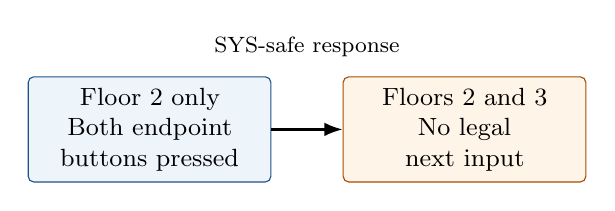
\begin{tikzpicture}[>=Latex,every node/.style={font=\small,align=center},
state/.style={draw,rounded corners=2pt,text width=2.8cm,minimum height=1.15cm,inner sep=4pt}]
\node[state,fill=softblue,draw=sourceblue] (before) at (0,0)
 {Floor 2 only\\Both endpoint\\buttons pressed};
\node[state,fill=softorange,draw=fliporange] (after) at (4.0,0)
 {Floors 2 and 3\\No legal\\next input};
\draw[->,thick] (before.east)--(after.west);
\node[font=\footnotesize] at (2,1.05) {SYS-safe response};
\end{tikzpicture}
\caption{A source-safe Lift response makes the ENV-owned floor invariant
false. The returned graph fails cooperation; another policy for the same
source contract passes. Full source values and the initialized prefix
are in Supplement~H.}
\label{fig:si-lift-admission}
\end{figure}


A matched diagnosis supplies identical model, solve and stored fixed-point
memory to two extractions. A final-choice preference keeps candidates
with a legal next input when available, while retaining helper-true
candidates; progress, goal, existing-node and private-memory rules remain
fixed. Its 154-node graph passes both complete checks. The preference
also acts at first creation of a bad node (Supplements~H, T and W).

Selection is not the sole cause: the encoded arena already permits the
bad state. Moving the invariant to SYS/next makes both outputs pass but
changes ownership and timing together. Nor does immediate input
availability guarantee ENV fairness, as the constructed Polling control
shows (Supplement~O). The generic extractor has no established binding
to the prescribed cooperative rank/mode construction~\cite{friendly},
and Lift's raw arena fails its sufficient language premise
(Supplement~V). This fixed-output diagnosis does not refute that construction.

\subsection*{AB.2 Separate comparison groups}
The two fixed rosters supply admitted alternatives for all cooperatively
feasible contracts: 8 of 11 reconstructed listings and 12 of 14 public inputs.
Those are separate route runs, not matched extraction or comparative
superiority. Infeasible or correspondence-UNKNOWN examples remain in
the records (Supplements~H and T).

\begin{table}[t]
\centering\small
\caption{Supporting comparisons. An admitted graph passes complete strictness
and legal-prefix cooperation checks. Selection rules and denominators are separate.}
\label{tab:si-comparison-summary}
\begin{tabular}{@{}L{35mm}L{77mm}L{37mm}@{}}\toprule
Fixed group & Result & Meaning and full records\\\midrule
11 reconstructed listings, five published examples & Selected route:
7 admitted, 2 strict-only, 1 raw negative, 1 correspondence UNKNOWN.
Normalized: 8 admitted, 3 empty-region stops. & An admitted alternative
for each feasible listing; Supplement~H.\\[4pt]
14 certified public inputs, at most 4,096 states; no region/output filter &
56 input/route outcomes. Selected: 11 admitted, 2 strict-only, 1 UNKNOWN.
Each normalized/cooperative-Slugs route: 12 admitted, 2 negative.
Nonblocking strict: 12 admitted, 1 strict-only, 1 negative. &
Separate runs; no population or performance comparison; Supplement~T.\\[4pt]
59 certified models from the stopped 425-unit inventory &
49 satisfy $W\subseteq C$; 10 have strict losses. Nine exact-loss
calculations finish with no lost $K$ state; one UNKNOWN. All ten lack
cooperative initialization. & No confirmed cooperative-initialization
loss; Supplements~E and J.\\[4pt]
7 fixed cooperative-positive native controls~\cite{fixedsevennative2026} &
14 native queries, 198,672 typed-state comparisons: source $W$, prior
$W=K$ and route source view agree; both initial judgments true. &
3 helper-active, 4 identity/skip controls; no loss or gain; Supplement~Y.\\\bottomrule
\end{tabular}
\end{table}


\subsection*{AB.3 Historical Patrol reports and executed reuse}
For historical context, the original artifact reports
\code{4FP=TRUE} and \code{reduction+4FP=FALSE} for the byte-identical new
input, where 4FP means four fixed points~\cite{kindartifact}.
Those paired reports use a distinct historical driver; they establish
neither a current-tool reproduction nor a strict-semantic cause (Supplement~Z).

The checked source controller executes 67 new-mode commits without
resetting plant/controller objects, source fields, monitors or private
phase. It serves the initial request at step~30 and clears its monitor
at~31; a repeatable 35-step full-state/private-memory cycle meets all
eight source justices. The workload was fixed after diagnosis, before
execution. This is validated reuse in the constructed scenario.
The known complete first-change correction is another strict-preserving
alternative by theorem; a direct full-arena native source solve was not
run here (Supplements~S and U).

\subsection*{AB.4. Computation provenance}
This section retains the detailed audit and cohort account behind the
main paper's evidence summary. It introduces no new execution or result.

\paragraph{Named computations and separate checks.}

The preceding proofs explain the mechanisms. This section and the current
evidence index distinguish the computations that corroborate them from
other checks that remain incomplete. A result is always attached to a named game or
validation procedure. A solve computes a winning region. A saved-region
audit checks an existing result. A theorem certificate here derives the
claimed region from checked relations and an independently precomputed
source region; it does not solve the transformed game anew. An independent
fixed-point audit instead attempts to recompute the region.



\paragraph{Implementation and answer.}
The strict winning-region calculations use JTLV and Spectra release
\code{1.0.0.202402072123}~\cite{spectrarelease2024}. The headless syntactic conversion runs
before default translation and BDD construction. Static source and
bytecode inspection bind this conversion to the \emph{public opt-in Kind
option}; shipped defaults use ordinary GR(1). The winning-region queries
here use released \code{GR1Game} with strict semantics. They establish
answers for the checked games. Corresponding Kind frontend answers for
Vehicle and Patrol remain unobserved. Section~AC
reports two separate public Kind realizability checks for Obstacle.
AC.7 adds completed ordinary-GR(1) controls for the same exact A/B queries,
using JTLV with optimizations and reordering disabled. These use the
installed default synthesis mode; they do not test every default setting
or backend. Vehicle and Patrol have no corresponding public-mode
observations. The separate complete-correction class exists in the
release; its supported frontend invocation remains unestablished.

\emph{UNKNOWN} means that the named query or validation attempt did not
establish a definitive answer under its recorded stopping rule. It is
never a negative synthesis verdict. A native result can be saved while
a separate audit remains UNKNOWN. Unattempted work and processing
exceptions retain separate statuses and causes.



\paragraph{Dependencies and test objects.}
The checks bind typed domains, source predicates, initializers, ordered
justices and helper transitions to the queried relations. In Vehicle,
full relation checks establish the complete literal form; two evaluators
then inspect the same saved native sets. In Patrol, the hand proof uses
the displayed source equations, and separate full-domain export checks
establish the identities used in the main paper's Patrol section.
Obstacle also has source-equation winning regions computed before the
native candidates. A saved-set audit or theorem certificate does not
recompute a winning fixed point. Shared compiler exports and typed-domain
metadata remain dependencies of the corresponding checks
(Supplements~B, E, U, V, W, X and AC).

For Patrol, source-legal steps preserve the reached checkpoint layout.
The 4,800-state restriction covers source-legal prefixes; the first-change
test $F$ still uses every typed input, including relocated checkpoints,
through the full-domain relations. Writing $D_L$ for that closed source domain, exact calculations give
$|W\cap D_L|=3,280$ and $|W_F\cap D_L|=1,104$. A completed native $M_F$ query agrees with
a separate explicit calculation and membership audit on all states
(Supplements~U.1 and U.6). It corroborates the maintained-response
calculation. The loss in the actual helper game follows from the source
all-response proof, the checked export identities and
the main paper's retained-duty preservation proposition. Direct full-helper attempts remain UNKNOWN
and supply no observed refusal. Their distinct stopping records are
retained in Supplement~U.5.


\subsection*{AB.5. Wider comparisons and selection}

A stopped 425-unit inventory yielded 70 completed models and,
after eleven certification exclusions, 59 analyzed models without
outcome filtering. Ten have literal strict losses; all ten lack
cooperative initialization. Of nine completed exact-loss calculations,
seven have empty $K$ and two preserve all $K$ states; one remains UNKNOWN.
This cohort therefore confirms no cooperative-initialization loss.
Vehicle, Patrol~277 and the published Obstacle update pair all lie outside
this frozen cohort. The primary Patrol NEW source is byte-identical to
corpus~277 (Section~Z); its later case-specific proof does not change the
59-model denominator. At selection, Patrol had no eligible authoritative
independent region certificate: the recorded status was
\path{UNKNOWN_NO_AUTHORITATIVE_INDEPENDENT_W}, with prior status
\path{UNKNOWN_NATIVE_NOT_ARRIVED} and no BDD worker started for this
condition check. A separately recorded native attempt stopped at its raw-output
cap; that later resource UNKNOWN is not the cohort-selection reason.
The cohort is conditioned on completion and certification under the stopped
resource protocol, not a sample establishing corpus-wide incidence.

The remaining 49 cohort models satisfy $W\subseteq C$, so the literal
strict encoding preserves all their source winners. In the nine
completed exact-loss rows, $K\cap(W\setminus W_C)=\varnothing$:
seven have empty $K$, and the other two preserve every $K$ state.
Let $K_{\rm all}$ denote source states admitting Kind's all-history
cooperation requirement, as distinct from the legal-prefix set $K$ used
in this supplement. Since $K_{\rm all}\subseteq K$, these existing facts
exclude $K_{\rm all}\setminus W_C$ in 58 cohort models. The exact
intersection for the single remaining corpus model 159 (RoboticArm) is UNKNOWN.
This is a consequence for the literal strict target, not a zero-of-59
incidence result, a Kind-to-Kind preservation theorem, or an observation
about public Kind actions. The existing reachability relation uses legal
joint edges; it is not the reached set of a winning or deployed
controller and carries no private memory.

A conditioned eleven-source subset has 40 certified results and four
UNKNOWNs across 44 encoding variants. Four of ten certified syntactic
variants lose strict states, and two also lose strict initialization;
all four loss sources already lack cooperative initialization. All ten have
$U=D$. The checked first-change and complete corrections preserve
their source regions. Supplement~AA gives every variant and unresolved
operation. These conditioned comparisons supply no incidence estimate;
the small proper-$U$ example establishes a logical need, not its
frequency in those exports. Supporting comparisons and output diagnoses
are in Supplement~AB, and fixed-seven native controls in
Supplement~Y~\cite{fixedsevennative2026}. Claim-specific saved records and
scoped replays remain separately identified (see the current evidence index).


\subsection*{AB.6. Patrol route retained from the main paper}
The route shown is the source-policy witness used by the main paper's
Patrol proof. Its standoffs, waiting rule, counter/monitor behavior and
all-response loss argument retain their original scope. The main paper
specifies the coordinates and complete source rules directly.

\begin{figure}[!t]
\centering
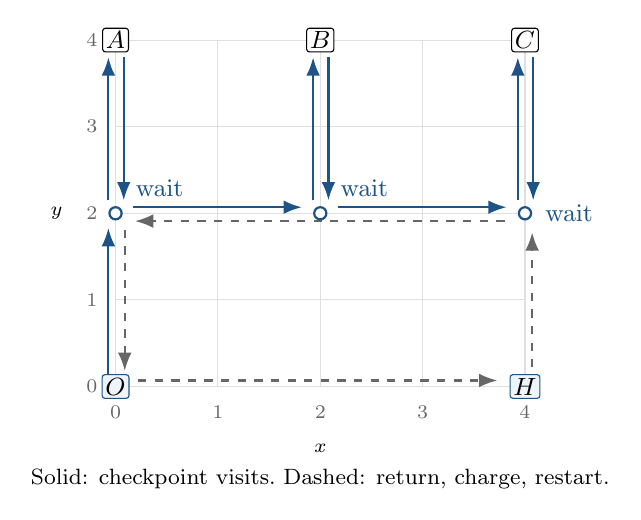
\begin{tikzpicture}[x=13mm,y=11mm,>=Latex,
 every node/.style={font=\small,inner sep=1.2pt},
 visit/.style={sourceblue,thick},
 charge/.style={black!60,thick,dashed}]
\draw[step=1,gray!25,thin] (0,0) grid (4,4);
\foreach \x in {0,...,4} {\node[below,text=black!60,font=\scriptsize] at (\x,-.18) {\x};}
\foreach \y in {0,...,4} {\node[left,text=black!60,font=\scriptsize] at (-.14,\y) {\y};}
\node[below,font=\scriptsize] at (2,-.62) {$x$};
\node[left,font=\scriptsize] at (-.48,2) {$y$};

% Source tour: rise to the first standoff, visit A/B/C, then return.
\draw[visit,->] (-.07,.12)--(-.07,1.83);
\draw[visit,->] (-.07,2.15)--(-.07,3.80);
\draw[visit,->] (.08,3.80)--(.08,2.15);
\draw[visit,->] (.17,2.07)--(1.82,2.07);
\draw[visit,->] (1.93,2.15)--(1.93,3.80);
\draw[visit,->] (2.08,3.80)--(2.08,2.15);
\draw[visit,->] (2.17,2.07)--(3.82,2.07);
\draw[visit,->] (3.93,2.15)--(3.93,3.80);
\draw[visit,->] (4.08,3.80)--(4.08,2.15);

% Return through row 2 and O, visit H, then restart at the first standoff.
\draw[charge,->] (3.80,1.91)--(.19,1.91);
\draw[charge,->] (.09,1.81)--(.09,.18);
\draw[charge,->] (.22,.07)--(3.73,.07);
\draw[charge,->] (4.07,.22)--(4.07,1.78);

\foreach \x in {0,2,4} {\filldraw[fill=white,draw=sourceblue,thick] (\x,2) circle (2.2pt);}
\node[fill=white,text=sourceblue,above right] at (.16,2.15) {wait};
\node[fill=white,text=sourceblue,above right] at (2.16,2.15) {wait};
\node[fill=white,text=sourceblue,right] at (4.16,2) {wait};
\node[draw,fill=white,rounded corners=1pt] at (0,4) {$A$};
\node[draw,fill=white,rounded corners=1pt] at (2,4) {$B$};
\node[draw,fill=white,rounded corners=1pt] at (4,4) {$C$};
\node[draw=sourceblue,fill=softblue,rounded corners=1pt] at (0,0) {$O$};
\node[draw=sourceblue,fill=softblue,rounded corners=1pt] at (4,0) {$H$};
\node[align=center,anchor=north,font=\footnotesize] at (2,-.91)
 {Solid: checkpoint visits.\ Dashed: return, charge, restart.};
\end{tikzpicture}
\caption{The source patrol route on the fixed $5\times5$ layout. The
robot waits two cells below each checkpoint, visits it when entry is
safe, then retreats. After $A,B,C$ it returns to $O$, visits charger $H$,
dwells, and returns along row~2 to the first waiting point.
The main paper's Patrol section gives the complete waiting, safety and fairness
argument. This source route witnesses feasibility; the loss proof covers
every safe strategy.}
\label{fig:patrol-map}
\end{figure}

\section*{AC. Published Obstacle Evasion requirements-update pair}
\subsection*{AC.1 Source provenance and the ordinary-game projection}
We use the exact old/update example distributed with Amram et al.'s
\emph{Dynamic Update for Synthesized GR(1) Controllers}~\cite{dupdate}.
The author site and source archive are
\url{https://smlab.cs.tau.ac.il/syntech/dupdate/} and
\url{https://smlab.cs.tau.ac.il/syntech/dupdate/Specifications.zip}.
The archive is 6,517 bytes; its SHA-256 is
\path{16483e1d023bdaea9201209639b67eb9b654ab367fa7eac51d62966f2b5916c4}.
The original files are
\path{Specifications/Obstacle Evasion/MovingObstacleEvasion.spectra} and
\path{Specifications/Obstacle Evasion/MovingObstacleEvasionUpdate.spectra}.
The old source hash is
\path{19c71d970b05fec41f0fa60fce155bf136b33836ffd785a65c2c436a712c3ac1};
the unprojected update source hash is
\path{bf2836d68e9a7b019b8f2c9499ccf1ad8dccdc56f5c31ff78ea7d80e45b1a228}.

The paper motivates changing forbidden and repeatedly visited robot
locations while avoiding a moving obstacle. Its update semantics replaces
old SYS goals. The old forbidden positions $(3,5),(4,5)$ become
$(6,4),(8,7)$; recurring targets $(5,2),(2,3)$ become $(3,7),(4,8)$.
ENV transitions and SYS movement/collision clauses are unchanged.
This is a published full-SYS requirements replacement, not an ENV-only
update, a same-pending-obligation continuation, or an observed industrial
workload. No link from this standalone pair to one particular pair in
the paper's larger evaluation is established.

The five scalar fields are obstacle coordinates in $1..7$, Boolean
\code{obsWait}, and robot coordinates in $1..8$, giving
$7^2\cdot2\cdot8^2=6,272$ typed states. No source monitor, pattern or AUX
field is declared. The old initializer fixes obstacle $(7,7)$,
\code{obsWait=false}, robot $(1,1)$. The update intentionally omits
initializers and declares the switch robot=$(5,5)$.
For the ordinary Spectra game parser, exactly the 45-byte switch declaration
is removed from the update; the remaining 1,902-byte source has hash
\path{be0eaddf7b165df254d417dcb8cfcd962307f859f1ac3d26514c4a26c4b3954b}.
The declaration remains boundary metadata, never an inserted initializer.
Old-source projection is identity. Independent source-to-export checks
cover domain, initializers, safety and ordered justices, including the
current/next component interpretation of array predicates.

\subsection*{AC.2 Region and initializer evidence}
The four registered arms are A: source, B: released syntactic helper,
C: release only the $0\to1$ SYS obligations, and D: existing complete
semantic correction. C leaves the other quadrants and initializer/justice
conditions of B unchanged. Both variants use the headless released
Spectra/JTLV route described in the main paper; these are strict games,
not the separate public Kind checks reported in AC.6 or a default GUI experiment.
The original source initializers, including their absence in the new
source, are preserved. Helper introduction binds initialization to $b=0$.

\begin{center}\small
\begin{tabular}{@{}llrrrrl@{}}\toprule
Source & Arm & $|W_R(\cdot,0)|$ & $|W_R(\cdot,1)|$ & Loss & Gain & Initial\\\midrule
old & A & 5,016 & -- & 0 & 0 & true\\
old & B & 0 & 6,272 & 5,016 & 0 & false\\
old & C & 5,016 & 6,272 & 0 & 0 & true\\
old & D & 5,016 & 6,272 & 0 & 0 & true\\
new & A & 5,015 & -- & 0 & 0 & true\\
new & B & 0 & 6,272 & 5,015 & 0 & false\\
new & C & 5,015 & 6,272 & 0 & 0 & true\\
new & D & 5,015 & 6,272 & 0 & 0 & true\\
\bottomrule\end{tabular}
\end{center}
For A, the first count means source $|W|$ and no helper is present.
Every helper-introducing arm has $U=D$.
For B, the one-step entry condition is $F=\varnothing$, so $W_F=\varnothing$.
For C and D, $F=D$ and $W_F=W$; every state membership, not just the
cardinality, agrees with the independently computed source region.
The difference between source counts 5,016 and 5,015 does not imply that
the regions differ in only one state.

The immediate obstruction is already in both sources. For current robot
$(x,y)$, choose next obstacle $(\min(x,7),\min(y,7))$. Its occupied
$2\times2$ square includes the current robot. The source
\code{robotAvoidsObstacle} clause compares the current robot against next
obstacle coordinates; it contains no next SYS variable. Thus some
avoidance conjunct is false for every response. Under B's checked first
change, that input is legal. C removes exactly the conflicting response
duty at that transition; its success here is not a universal sufficiency
claim when retained helper-true constraints may give proper $U$.

Both source ENV relations are total on typed states and have zero ENV
justice assumptions. After any legal prefix of a strict winner, its
residual remains winning and ENV has a next legal input. Repeatedly choosing
legal inputs supplies an infinite legal continuation; the empty ENV
justice conjunction holds automatically. Hence $W\subseteq K$, and
$K\subseteq W$ by definition: $K=W$ for both sources. Independently
enumerating the authored initializer quantifiers gives
$I_M(K)=I_M(W)=\mathit{true}$ in each, but false initialization for B.
This argument establishes the paper's legal-prefix cooperation.
Section~AC.5 separately proves the stronger all-history property for
these source contracts. Neither argument identifies the result of a
raw four-fixed-point implementation.

\subsection*{AC.3 A sealed old-only prefix and the complete switch roster}
Before any source/compiler/solver calculation, the published switch
robot=$(5,5)$ was completed with all 98 obstacle/\code{obsWait} valuations
in fixed lexicographic order. No winning, reachability, safety or
initializer filter changes that denominator. Source initialization is
not reapplied at the replacement boundary.

Using only the old source and old $W$, a FIFO search with lexicographic
ENV/SYS edges selected the following seven-edge legal prefix and sealed
it before new-source evaluation. Every state is old-winning. The terminal
state is also new-winning and belongs to new A/C/D, but not B.
This establishes a possible old winning prefix; it does not establish an
extracted controller, its private memory or an installed handoff.

\begin{center}\small
\begin{tabular}{@{}rrrrr@{}}\toprule
Step & Obstacle & \code{obsWait} & Robot & Source ID\\\midrule
0 & $(7,7)$ & false & $(1,1)$ & 6144\\
1 & $(6,6)$ & true & $(1,2)$ & 5185\\
2 & $(6,6)$ & false & $(1,3)$ & 5122\\
3 & $(5,5)$ & true & $(1,4)$ & 4163\\
4 & $(5,5)$ & false & $(2,5)$ & 4108\\
5 & $(4,6)$ & true & $(3,4)$ & 3411\\
6 & $(4,6)$ & false & $(4,4)$ & 3355\\
7 & $(3,5)$ & true & $(5,5)$ & 2404\\
\bottomrule\end{tabular}
\end{center}
The complete boundary partitions into 48 old-W-prefix-reachable states
winning in both sources, 30 states winning in both but not old-W-prefix
reachable, and 20 states outside both winning sets. The 30 are not an
old/new winning-region discrepancy. In each variant A/C/D accept the
same 78 boundary states and B accepts zero. The obstruction is present
before and after the update; these results do not show update-caused loss.

The following table lists every frozen completion. Robot is $(5,5)$
throughout. ``W/ACD'' means membership in both source regions and all
six helper-false A/C/D source views; these are identical for these 98 rows.
``Reach'' means old-W-prefix reachability. All 98 helper-false B entries
are false in both variants; all helper-true B/C/D entries are true.
Thus the table and these constants specify all 784 source/helper-false arm memberships.

{\small
\begin{longtable}{@{}rrrrrr@{}}
\toprule No. & Obstacle & \code{obsWait} & Source ID & W/ACD & Reach\\\midrule
\endfirsthead
\toprule No. & Obstacle & \code{obsWait} & Source ID & W/ACD & Reach\\\midrule
\endhead
\bottomrule\endfoot
1 & $(1,1)$ & 0 & 36 & 1 & 0\\
2 & $(1,1)$ & 1 & 100 & 1 & 0\\
3 & $(1,2)$ & 0 & 164 & 1 & 0\\
4 & $(1,2)$ & 1 & 228 & 1 & 0\\
5 & $(1,3)$ & 0 & 292 & 1 & 1\\
6 & $(1,3)$ & 1 & 356 & 1 & 0\\
7 & $(1,4)$ & 0 & 420 & 1 & 1\\
8 & $(1,4)$ & 1 & 484 & 1 & 0\\
9 & $(1,5)$ & 0 & 548 & 1 & 1\\
10 & $(1,5)$ & 1 & 612 & 1 & 0\\
11 & $(1,6)$ & 0 & 676 & 1 & 0\\
12 & $(1,6)$ & 1 & 740 & 1 & 0\\
13 & $(1,7)$ & 0 & 804 & 1 & 0\\
14 & $(1,7)$ & 1 & 868 & 1 & 0\\
15 & $(2,1)$ & 0 & 932 & 1 & 0\\
16 & $(2,1)$ & 1 & 996 & 1 & 0\\
17 & $(2,2)$ & 0 & 1060 & 1 & 1\\
18 & $(2,2)$ & 1 & 1124 & 1 & 1\\
19 & $(2,3)$ & 0 & 1188 & 1 & 1\\
20 & $(2,3)$ & 1 & 1252 & 1 & 1\\
21 & $(2,4)$ & 0 & 1316 & 1 & 1\\
22 & $(2,4)$ & 1 & 1380 & 1 & 1\\
23 & $(2,5)$ & 0 & 1444 & 1 & 1\\
24 & $(2,5)$ & 1 & 1508 & 1 & 1\\
25 & $(2,6)$ & 0 & 1572 & 1 & 1\\
26 & $(2,6)$ & 1 & 1636 & 1 & 1\\
27 & $(2,7)$ & 0 & 1700 & 1 & 0\\
28 & $(2,7)$ & 1 & 1764 & 1 & 0\\
29 & $(3,1)$ & 0 & 1828 & 1 & 1\\
30 & $(3,1)$ & 1 & 1892 & 1 & 0\\
31 & $(3,2)$ & 0 & 1956 & 1 & 1\\
32 & $(3,2)$ & 1 & 2020 & 1 & 1\\
33 & $(3,3)$ & 0 & 2084 & 0 & 0\\
34 & $(3,3)$ & 1 & 2148 & 1 & 1\\
35 & $(3,4)$ & 0 & 2212 & 0 & 0\\
36 & $(3,4)$ & 1 & 2276 & 1 & 1\\
37 & $(3,5)$ & 0 & 2340 & 0 & 0\\
38 & $(3,5)$ & 1 & 2404 & 1 & 1\\
39 & $(3,6)$ & 0 & 2468 & 0 & 0\\
40 & $(3,6)$ & 1 & 2532 & 1 & 1\\
41 & $(3,7)$ & 0 & 2596 & 1 & 1\\
42 & $(3,7)$ & 1 & 2660 & 1 & 1\\
43 & $(4,1)$ & 0 & 2724 & 1 & 1\\
44 & $(4,1)$ & 1 & 2788 & 1 & 0\\
45 & $(4,2)$ & 0 & 2852 & 1 & 1\\
46 & $(4,2)$ & 1 & 2916 & 1 & 1\\
47 & $(4,3)$ & 0 & 2980 & 0 & 0\\
48 & $(4,3)$ & 1 & 3044 & 1 & 1\\
49 & $(4,4)$ & 0 & 3108 & 0 & 0\\
50 & $(4,4)$ & 1 & 3172 & 0 & 0\\
51 & $(4,5)$ & 0 & 3236 & 0 & 0\\
52 & $(4,5)$ & 1 & 3300 & 0 & 0\\
53 & $(4,6)$ & 0 & 3364 & 0 & 0\\
54 & $(4,6)$ & 1 & 3428 & 1 & 1\\
55 & $(4,7)$ & 0 & 3492 & 1 & 1\\
56 & $(4,7)$ & 1 & 3556 & 1 & 1\\
57 & $(5,1)$ & 0 & 3620 & 1 & 1\\
58 & $(5,1)$ & 1 & 3684 & 1 & 0\\
59 & $(5,2)$ & 0 & 3748 & 1 & 1\\
60 & $(5,2)$ & 1 & 3812 & 1 & 1\\
61 & $(5,3)$ & 0 & 3876 & 0 & 0\\
62 & $(5,3)$ & 1 & 3940 & 1 & 1\\
63 & $(5,4)$ & 0 & 4004 & 0 & 0\\
64 & $(5,4)$ & 1 & 4068 & 0 & 0\\
65 & $(5,5)$ & 0 & 4132 & 0 & 0\\
66 & $(5,5)$ & 1 & 4196 & 0 & 0\\
67 & $(5,6)$ & 0 & 4260 & 0 & 0\\
68 & $(5,6)$ & 1 & 4324 & 1 & 1\\
69 & $(5,7)$ & 0 & 4388 & 1 & 1\\
70 & $(5,7)$ & 1 & 4452 & 1 & 1\\
71 & $(6,1)$ & 0 & 4516 & 1 & 0\\
72 & $(6,1)$ & 1 & 4580 & 1 & 0\\
73 & $(6,2)$ & 0 & 4644 & 1 & 1\\
74 & $(6,2)$ & 1 & 4708 & 1 & 1\\
75 & $(6,3)$ & 0 & 4772 & 0 & 0\\
76 & $(6,3)$ & 1 & 4836 & 1 & 1\\
77 & $(6,4)$ & 0 & 4900 & 0 & 0\\
78 & $(6,4)$ & 1 & 4964 & 1 & 1\\
79 & $(6,5)$ & 0 & 5028 & 0 & 0\\
80 & $(6,5)$ & 1 & 5092 & 1 & 1\\
81 & $(6,6)$ & 0 & 5156 & 0 & 0\\
82 & $(6,6)$ & 1 & 5220 & 1 & 1\\
83 & $(6,7)$ & 0 & 5284 & 1 & 0\\
84 & $(6,7)$ & 1 & 5348 & 1 & 0\\
85 & $(7,1)$ & 0 & 5412 & 1 & 0\\
86 & $(7,1)$ & 1 & 5476 & 1 & 0\\
87 & $(7,2)$ & 0 & 5540 & 1 & 0\\
88 & $(7,2)$ & 1 & 5604 & 1 & 0\\
89 & $(7,3)$ & 0 & 5668 & 1 & 1\\
90 & $(7,3)$ & 1 & 5732 & 1 & 1\\
91 & $(7,4)$ & 0 & 5796 & 1 & 1\\
92 & $(7,4)$ & 1 & 5860 & 1 & 1\\
93 & $(7,5)$ & 0 & 5924 & 1 & 1\\
94 & $(7,5)$ & 1 & 5988 & 1 & 1\\
95 & $(7,6)$ & 0 & 6052 & 1 & 0\\
96 & $(7,6)$ & 1 & 6116 & 1 & 0\\
97 & $(7,7)$ & 0 & 6180 & 1 & 0\\
98 & $(7,7)$ & 1 & 6244 & 1 & 0\\
\end{longtable}}

\subsection*{AC.4 Independent certificate, retained failures and limits}
The evidence in this subsection is a distinct post-hoc theorem certificate
for saved native regions. Section~AC.7 adds later positive rank/response
witnesses and ordinary-mode controls without changing these records. Independent source-equation winning regions were computed
before the native candidates. Exact canonical-Boolean correspondence
checks bind source predicates, typed fields, initializers, ordered justices,
helper quadrants and immutable snapshot identities. The certificate proves
$U=D$ from typed $S_{11}$ totality, computes one $\CPre_{01}(D)$ per
helper arm, and uses only the sufficient endpoints $F=\varnothing$ or
$F=D$. It never substitutes $W\cap F$ for $W_F$ at a proper $F$.
All typed source/helper states and all Boolean current-state encodings
are checked, including raw/typed/domain/helper-false export masks.
Initializer enumeration uses one SYS response satisfying both its
initializer and winning membership for each admissible initial ENV value.

All eight certificates pass. The method performs six one-step predecessor
calls but no new native/source solve or fixed-point iteration. It was
introduced after observing native candidates and resource caps, so it is
not a preregistered replacement or an independently recomputed transformed
fixed point. The eight original independent fixed-point attempts retain
UNKNOWN at the fixed 500,000-node limit. A first distinct certificate
attempt retains an old/A serialization exception and seven not-attempted
slots. A separately authorized amendment removes the duplicate output
keyword and repeats the fixed eight certificates without changing the
earlier evidence or its status. Independent pre-execution and result
reviews check that separation and the interpretation of the saved records.

Saved records include \path{FINAL_CERTIFICATE_SUMMARY.json},
\path{FINAL_CERTIFICATE_TABLE.csv}, \path{ALL98_FIXED8_MEMBERSHIP.json},
\path{ALL98_FIXED8_MEMBERSHIP.csv}, and per-arm certificates, membership
tables and process receipts. The frozen-input manifest, source/native
outputs, original failures and all subsequent checks remain available
alongside the fixed protocol. This is one published example pair, not
prevalence, external reproduction, comparative performance, default
frontend behavior or demonstrated deployment. No controller extraction
or private-memory transfer is inferred from finite source-state prefixes.


\subsection*{AC.5 Source strict winning and all-history kindness}
The legal-prefix requirement used for $K$ is generally weaker than
Kind's Definition~3~\cite{kind}. That definition additionally asks for an
ENV-safe, ENV-fair continuation from every position of a play induced by
the winning system strategy and an arbitrary ENV strategy, including
histories after an ENV violation. The continuation uses the same residual
system strategy. It does not reapply the source initializer or repair the
already elapsed prefix. For the two Obstacle sources, the following
argument establishes this stronger property.

\paragraph{Lemma (total ENV safety without ENV justice).}
Consider a finite Mealy source with nonempty typed domain $D=E\times Y$.
Assume that $\rho_e(s,e')$ does not depend on the next SYS response and
that every $s\in D$ admits at least one $e'$ satisfying $\rho_e(s,e')$.
The latter condition is required on all typed states, not merely on $W$.
Assume that the ENV justice list is empty, or contains only identically
true padding. Let $S$ be a strict-winning source strategy. If initially
partial, extend it to a strategy $\bar S$ returning a typed response on
every typed history. The extension must preserve its initial response
for every input satisfying $\theta_e$, and its responses and ordinary
memory updates on histories where the original strict duties apply.
For an already total $S$, take $\bar S=S$. Then $\bar S$ satisfies the
additional all-history requirement of
Kind's Definition~3. Consequently, strict-winning and kind strategy
existence coincide for this source.

\begin{proof}
Choose a legal ENV selector $f:D\to E$ with
$\rho_e(s,f(s))$ for every $s\in D$. Such a selector exists by finiteness
and totality. Fix any history $h=(s_0,\ldots,s_i)$ induced by $\bar S$
and any ENV strategy. The history may contain an ENV initializer or
safety violation. From position $i$ onward, choose
$e_{t+1}=f(s_t)$ and let SYS use
\[
 y_{t+1}=\bar S_T(s_0,\ldots,s_i,\ldots,s_t,e_{t+1}).
\]
This retains the full prefix and the strategy memory reached along it;
it neither invokes the initial selector again nor resets memory.
Next-response independence means that SYS cannot falsify the chosen
ENV edge. Typed totality puts the successor back in $D$, so the same
argument can repeat indefinitely. The resulting suffix is ENV-safe,
and the empty or identically true ENV justice list makes it ENV-fair.
The construction works from every induced history and position.

Strict realizability is preserved because the extension leaves the
initial output and all responses carrying strict duties unchanged.
An initially invalid ENV input disables those duties; after a first
ENV safety violation, arbitrary typed completion creates no new strict
SYS safety or justice obligation. This does not erase initial or
pre-violation duties already incurred. Thus $\bar S$ remains strict-winning
and satisfies the additional kindness condition. The converse follows
because Definition~3 already requires strict winning.
\end{proof}

The source strategy functions in the primary definition are already
total. The completion condition states what is needed when starting
from a partial implementation. It does not require a safe SYS response
at every typed state: after an ENV violation the strict source duties
have been released. An implementation that instead stops there is not
thereby certified as a typed-total strategy.

\paragraph{A selector for both Obstacle sources.}
Let $o=(o_0,o_1)\in\{1,\ldots,7\}^2$ be the obstacle position,
$p=(p_0,p_1)\in\{1,\ldots,8\}^2$ the current robot position, and
$w=\code{obsWait}$. If $w$ is true, keep $o'=o$ and set $w'=\mathit{false}$.
Otherwise set $w'=\mathit{true}$ and, independently for each coordinate,
choose
\[
 o_j'=\begin{cases}
 o_j-1,&o_j>p_j,\\
 o_j+1,&o_j<p_j-1,\\
 o_j,&\text{otherwise}.
 \end{cases}
\]
The decrement case has $o_j\ge2$; the increment case has $o_j\le6$.
Both stay within $1..7$ and move by at most one. In the remaining case,
$p_j-1\le o_j\le p_j$, so neither directed-motion antecedent applies.
Together with the wait flag choice, these cases satisfy every ENV
wait, motion and directed-motion clause. They use only current robot
coordinates, not the next SYS response. This proves totality over all
6,272 typed states without assuming source winning or reachability.
The old and new sources have the same ENV transition relation and empty
ENV justice lists. Their initializers differ: the old ENV initializer
fixes $o=(7,7),w=\mathit{false}$; the new source has no ENV initial
restriction.

\paragraph{Application and boundary.}
The existing strict source results therefore establish kind strategy
existence for both authored initializers. The retained state
$r=(o=(3,5),w=\mathit{true};p=(5,5))$, source ID~2404, belongs to both
source winning regions. The lemma also applies to a separately defined
continuation query fixing that current state. This does not reset to the
old initializer, construct an installed controller, or establish a
private-memory transfer. The proof preserves the residual memory of the
chosen strategy; it says nothing about an arbitrary existing controller
memory.

This is a source-game argument. Helper conversion adds
$\G\F\neg b$: at $b=1$, the one-way safety rule prevents any ENV-safe
suffix satisfying that justice. The lemma therefore does not apply to
the transformed game. It neither equates a raw four-fixed-point result
$Q$ with source $W$ or $K$, nor establishes a frontend answer or an
extracted controller's correctness. The strengthening above is a
mathematical consequence of the existing source relations and strict
results, not a new solver execution.

\clearpage
\subsection*{AC.6 Two fixed public Kind realizability checks}
The source-kind lemma permits a comparison beyond ordinary strict
winning: both queries below admit a strategy satisfying the all-history
source requirement of Kind's Definition~3. We separately tested the
published tool's \emph{Check Realizability} action on those fixed inputs.
Both returned \emph{Specification is unrealizable}. This is an observed
answer from a selected public checking path, not a new strict-region
certificate or a controller-handoff experiment.

\paragraph{Queries and exact initial meaning.}
The first query uses the unchanged 2,097-byte published old source from
AC.1. Its ENV initializer fixes obstacle $(7,7)$ and
$\mathit{obsWait}=\mathit{false}$; its SYS initializer fixes robot $(1,1)$.
The joint state is source ID~6144 and belongs to the accepted old winning
region. The ENV initial domain is nonempty, and the required initial
response exists for its sole input. Thus the initialized existence
claim retains the universal-ENV/existential-SYS initial quantifiers.

The second query uses the 1,902-byte ordinary projection of the update,
followed by this fixed 124-byte appendix:
\begin{lstlisting}
asm retainedBoundaryEnv:
obstacle[0] = 3 & obstacle[1] = 5 & obsWait;
gar retainedBoundarySys:
robot[0] = 5 & robot[1] = 5;
\end{lstlisting}
It fixes exactly the previously selected state
$r=(o=(3,5),w=\mathit{true};p=(5,5))$, source ID~2404, without conjoining
the old initializer. The input is 2,026 bytes, with SHA-256
\path{212309df489c3ddc7bf7ec6a750aed2d0da4fb7e26995e5ee3a0405c9897e1d5}.
Its first 1,902 bytes are identical to the accepted update projection;
all noninitial source clauses are unchanged. It is not the byte-unchanged
public update, nor an execution of that file's switch declaration.
The seven-edge old-only prefix in AC.3 fixed this endpoint before
new-source evaluation. No input was changed in response to a GUI result.

The accepted new strict region contains $r$. Applying AC.5 to this
separately initialized source query establishes a kind continuation.
The lemma retains the full history and residual memory of the chosen
strategy; it does not show that an arbitrary installed old controller's
memory is suitable for the new strategy. No such old-controller memory
was extracted or transferred.

\paragraph{Binding the point query to the accepted predicates.}
Before the second public action, a separate NoIDE export generated
saved predicates for the fixed input without constructing a solver or
computing a winning fixed point. A saved-data comparison checked the
source clause inventory, full ENV/SYS safety relations, typed domains,
all four helper-transition quadrants, ordered justices, and the
helper-false source relation against the accepted records. The ENV and
SYS initial predicates were each nonempty; their conjunction fixed
exactly $r$ with helper false. The point initializer therefore does not
obtain a result through an empty initial domain or an old-source restart.

The export supervisor nevertheless ended with
\path{UNKNOWN_SUPERVISOR_EXCEPTION}: its final process snapshot raced
with process exit. The OS return code was not recorded and is not
inferred to be zero. That original status remains unchanged. Before
the GUI action, a separate review adopted the saved mathematical objects
after checking their structure, predicate equality and complete capture:
257 checks and 55 pinned files passed in that review. This was a
saved-data acceptance, not a conversion of the supervisor record into
PASS. It ran no new Java process, model generation, solver or fixed point.

The NoIDE exporter and Eclipse use the same pinned release translator
but different resource providers and Java versions (17.0.19 and 17.0.9).
No live GUI BDD model was exported. The saved predicate correspondence
is therefore not an observation that every internal GUI predicate is
identical to the NoIDE export.

\paragraph{Selected public path and completed observations.}
Both actions used the installed Spectra release
\code{1.0.0.202402072123}, Kind selected by
\code{synthesisPitermanReduction}, JTLV, no optimizations and no
reordering. The public command was \code{tau.smlab.syntech.checkRealAction}.
The installed source and saved bytecode identify the static path: the shipped
syntactic reduction precedes the default translators, and the recorded JTLV
branch invokes \code{GR1SeparatedGame}. Both actual consoles displayed that
class and \code{JTLVJavaFactory 1.3}. The separate complete-correction class
represented by $R^+$ is not selected on this path. Section~AE.1 distinguishes
this static fact from live-model equality and runtime class origins.

\begin{center}\small
\begin{tabular}{@{}L{57mm}L{37mm}L{49mm}@{}}\toprule
Fixed query & Source existence evidence & Public observation\\\midrule
Old source, authored initialization &
Strict source certificate plus AC.5 &
Unrealizable; 1,011 ms\\[3pt]
Updated projection, point initialization at $r=2404$ &
Strict source certificate at $r$ plus AC.5 &
Unrealizable; 745 ms\\\bottomrule
\end{tabular}
\end{center}
Each input received one public action, with no retry and no controller
extraction. The times are plugin diagnostic computation times, not a
performance benchmark. Exact input snapshots, final settings, full
console screenshots, action logs, release-file checks and completion
records bind the observations. Separate read-only completion audits
found no discrepancy.

The old-input logger has one start/done pair and two identical source
snapshots. The retained-query logger has one start/done pair in one XML
file and one archived source snapshot; its same-second storage does not
provide two independently retained snapshots. That snapshot and the
prepared/current input all match the fixed hash above. Both GUI runs
completed without a recorded exception or resource-stop signal. These
GUI completion records are separate from the earlier export supervisor's
UNKNOWN and do not alter it. Console text is a visual transcription of
the unedited screenshots, not text obtained from the accessibility API.

\paragraph{Decision consequence and limits.}
For the old original initialization and for the fixed updated point
query, source-kind strategy existence is established independently of
the observed Boolean answers. If the selected public path is used as a
source-level continuation-feasibility gate at $r$, its false answer
would reject a continuation whose existence is separately proved.
This comparison does not rely only on the weaker legal-prefix set $K$.
The finite old prefix identifies a possible reached source valuation;
it does not establish a running old controller, its private memory,
an installed update, or an actual deployment rejecting the candidate.

The old query was already negative, so the update is not shown to
introduce the obstruction. The two observations neither export an
all-state raw four-fixed-point region $Q$ nor identify $Q$ with $W$ or
$K$. The headless correction certificates remain separate evidence for
the strict-game mechanism; the GUI observations do not isolate one
internal defect as the exclusive cause. They establish neither default
or all-backend behavior, incidence, deployment benefit, nor tool-author
intent. The eight earlier independent fixed-point UNKNOWNs and the
certificate-processing exception with seven then-unattempted slots in
AC.4 remain unchanged.

\subsection*{AC.7 Direct-source strategy certificates and matched public controls}
\label{supp:r6-obstacle-certificates}

\paragraph{Scope and exact queries.}
This additional study supplies explicit positive strategy certificates for
the same two initialized queries used in AC.6, and ordinary-GR(1) public
controls on the same input bytes. These are separate from the earlier
saved-region/theorem certificates in AC.4.
Query A is the unchanged 2,097-byte published old source, initialized at
$(o=(7,7),w=\mathit{false};p=(1,1))$.
Query B is the 2,026-byte retained-point update query, initialized at
$(o=(3,5),w=\mathit{true};p=(5,5))$.
Both start the certificate strategy in phase zero.

The checker binds the exact source length, SHA-256, case name, explicit
query tuple and initial tuple. Its separate source-binding check also
confirms the byte identities: A equals published old; the 1,947-byte
published update equals the 1,902-byte ordinary projection plus its
45-byte switch suffix; B equals that projection plus the fixed 124-byte
point initializer. Thus B preserves all noninitial source clauses and
does not conjoin the old initializer. These identities do not execute
the switch declaration or prove a controller handoff.

\paragraph{An independently implemented source checker.}
The checker imports only Python standard-library modules. It transcribes
the original source equations directly and imports no generator module,
old source evaluator, predecessor or fixed-point routine, saved graph,
or candidate-winning-set truth. Certificate provenance is informational,
not a proof premise. Its independence is from those implementations;
the mathematical argument still depends on the correctness of the
source transcription, the adopted declaration semantics, the checker
and its runtime. This is not an independent general-purpose Spectra
compiler.

The explicit state tuple is $(o_0,o_1,w,p_0,p_1)$, with obstacle coordinates
in $1..7$, a Boolean wait flag, and robot coordinates in $1..8$.
There are 98 typed ENV valuations, 64 typed SYS valuations and 6,272
typed states. Integer and Boolean types are checked separately.
The ENV predicate is the complete conjunction of wait alternation,
waiting-position persistence, obstacle movement by at most one per
coordinate, and the four
directed-motion implications listed in AC.5.

For SYS, the checker verifies current-state collision avoidance and
the two authored forbidden-location safety clauses: $(3,5),(4,5)$ for A,
and $(6,4),(8,7)$ for B. The declarations named
\path{AvoidInfinitely} are globally enforced safety clauses, despite
their names. Transition checks limit each robot coordinate's change
to at most one and preserve
\code{robotAvoidsObstacle}, which tests the \emph{current} robot against
the \emph{next} obstacle. Closure also checks successor current-state
safety, hence the next robot against the next obstacle. These are
distinct obligations. The two recurring SYS goals, in source order,
are $(5,2),(2,3)$ for A and $(3,7),(4,8)$ for B. Both ENV justice lists
are empty.

\paragraph{Certificate obligations and the winning argument.}
A certificate supplies a nonempty set $R$ of explicit typed states,
one bit of goal phase $q\in\{0,1\}$, two integer rank functions, and
one SYS response for each legal ENV input at each state and phase.
Ranks lie in $0..6271$; only finite nonnegative values are needed for
the well-foundedness argument. Write $G_q$ for the current phase's
source goal. The checker requires
$\operatorname{rank}_q(s)=0$ exactly when $s\in G_q$.

For each $s\in R$ and each phase, the checker independently enumerates
all 98 typed next ENV tuples. The supplied response keys must equal
the entire set satisfying the source ENV predicate: missing, duplicate
or extra inputs are rejected. This legal-input set must be nonempty.
Every response is typed, satisfies the complete source SYS transition
relation, and reaches a state $s'\in R$. Outside $G_q$, it must retain
phase $q$ and satisfy
\[
 \operatorname{rank}_q(s')<\operatorname{rank}_q(s).
\]
At $G_q$, the next phase must be $1-q$; no descent is required across
that phase change.

Consequently, every source-legal play stays safe in $R$. A phase cannot
avoid its goal forever, because that would produce an infinite strictly
decreasing sequence of nonnegative integers. The next step changes
phase, and the same argument repeats, giving infinitely many visits
to both source goals. This covers every legal ENV branch, not a
selected execution or merely one cycle.

Initialization is checked separately over all 98 ENV assignments and,
for each allowed initial ENV value, all 64 SYS assignments. Every
allowed ENV value must have a source-initial SYS witness in $R$.
Both exact queries have one admissible initial pair, present with
phase zero. The accepted results are:
\begin{center}\small
\begin{tabular}{@{}lrrrrl@{}}\toprule
Query & $|R|$ & \shortstack{Policy edges\\over two phases} &
Maximum rank & Initial pairs & Checker result\\\midrule
A & 5,016 & 12,656 & 17 & 1 & accept\\
B & 5,015 & 12,672 & 17 & 1 & accept\\\bottomrule
\end{tabular}
\end{center}
Both receipts report \path{ACCEPT_POSITIVE_EXISTENCE}.
They certify positive strategy existence for the exact queries and
the checked strategy on $R$. They do not prove that $R$ is a maximal
winning region or exclude any state outside it. The coincidence of
these cardinalities with the earlier region counts does not change
that scope; complete-region claims retain their earlier computational
premises.

\paragraph{Typed completion and the separate all-history bridge.}
The strategy has an ENV-violation latch in addition to the goal phase.
Both are private strategy memory, not additional source variables.
On an invalid ENV initial value or after the first ENV safety violation,
it latches the violation and forever returns typed SYS value $(1,1)$
with phase zero; it does not resume the certificate when ENV later
becomes legal. Otherwise unreachable histories use the same specified
fallback. The checked policy applies throughout every induced legal
prefix, preserving valid initial outputs and all responses and ordinary
memory updates carrying strict duties. Completion creates no new
SYS safety obligation after an ENV violation and erases none already owed.

The positive winning check does \emph{not} itself prove global ENV
totality. A separate check, bound to both exact sources, enumerates all
6,272 typed states and all 98 next ENV tuples at each state, including
states outside $R$ and states reachable by fallback. It reports
\path{ACCEPT_SOURCE_ENV_TOTALITY_ONLY}: 9,536 legal ENV edges, with
minimum outdegree one and maximum nine. The source ENV relation is
independent of the next SYS response and has no justice assumptions.

Combining this totality result with the typed-total certificate strategy
and AC.5 gives the source-specific all-history Kind property: after any
induced history, repeatedly select a legal ENV input while retaining
the same strategy, full prefix and reached phase/latch memory. Typed
successors remain in the domain, so this yields an ENV-safe infinite
suffix; empty ENV justice makes it fair. Initialization is not restarted.
The strict positive certificate and the ENV-totality argument are
logically separate premises. Neither supplies a general Kind-preservation
theorem or transfers arbitrary memory from an installed old controller.

\paragraph{Fixed malformed-certificate qualification.}
Two unmodified positive controls were accepted. For each source, the
frozen qualification roster supplied 25 malformed certificates; all
50 were rejected with their expected reason codes. The roster covers:
\begin{center}\small
\begin{tabular}{@{}L{30mm}L{100mm}r@{}}\toprule
Group & Mutations & Per source\\\midrule
ENV coverage &
Missing input, extra illegal input, duplicate input & 3\\
Safety and closure &
Unsafe robot step, unsafe current state, missing successor & 3\\
Ranks &
Negative, oversized or Boolean rank; zero off goal; no decrease & 5\\
Phase &
Wrong phase, phase stuck at a goal, missing phase policy & 3\\
Query binding &
Wrong query, case, source hash or source path; initial state missing & 5\\
Value types &
Integer wait value, Boolean SYS coordinate & 2\\
State and schema &
Duplicate state, extra metadata key, duplicate JSON key & 3\\
Completion &
Wrong completion declaration & 1\\\bottomrule
\end{tabular}
\end{center}
These checks measure observed rejection sensitivity of this fixed
roster, not complete checker correctness and not negative source
realizability.

Forty-eight rejection receipts directly contain the checked input hash.
The two duplicate-JSON-key inputs fail during parsing before the input
hash is returned to the receipt, leaving \path{certificate_sha256}
null. Their retained compressed inputs were checked against the exact
frozen mutation construction and the qualification driver's archive
hashes; the saved receipts and output report
\path{DUPLICATE_JSON_KEY}. Thus those two rejections have an explicit
driver/input provenance chain, not a populated receipt input-hash field.

Six frozen supervised stages completed once each: the two generations,
the two positive checks, the separate totality/binding check, and
qualification. Each positive-check stage and the totality/binding stage
had 180-second wall and per-process CPU budgets. The qualification stage had
300-second wall and per-process CPU budgets. The owned-process
supervisor monitored the process tree against a 1-GiB sampled RSS budget.
RSS samples, particularly for short stages with only two samples, do
not establish instantaneous peak memory or a continuous hard RSS bound.
These records support no performance claim.

\paragraph{Matched public ordinary-GR(1) controls.}
Using the same A/B bytes and installed release as AC.6, the public
\emph{Check Realizability} action was run once per query in
\emph{Original GR(1)} mode, with JTLV, optimizations disabled and
reordering disabled. Both answers were \emph{Specification is realizable}.
The previous selected Kind-mode answers remain false:
\begin{center}\small
\begin{tabular}{@{}llll@{}}\toprule
Query & Ordinary GR(1) & Previous Kind & Ordinary console time\\\midrule
A & true, one action & false, one action & 10,391 ms\\
B & true, one action & false, one action & 14,221 ms\\\bottomrule
\end{tabular}
\end{center}
The times are diagnostic provenance, not a benchmark.
The ordinary consoles identify \path{GR1GameMemoryless},
\code{JTLVJavaFactory 1.3}, and the diagnostics
\code{env 7 / sys 6 / aux 0}. Exact source archives, one start/done XML
pair per query, screenshots and owned-process monitoring bind the
observations. The preference UI, installed default-initializer bytecode
and runtime console establish ordinary-mode selection; the serialized
\code{synthesisMethod} preference is absent because ordinary GR(1) is
the installed default.

This is a matched-input mode contrast. Mode selection changes both
reduction and solver, so the contrast does not isolate one exclusive
internal cause. No live GUI intermediate BDD or predicate export was
obtained. The installed-code mapping and saved source correspondence
are distinct from observing those live intermediate predicates.
A was already negative in Kind mode; the update is not shown to
introduce that obstruction.

\paragraph{Evidence identity and retained limits.}
The checker file \path{check_certificate.py} has SHA-256
\path{9618f0cbbe7dafb92f963e200f2304f802629aef248f563de0e039eda23ce28d};
the qualification driver \path{qualify_rejections.py} has SHA-256
\path{4ff6c3beb4e04050e87b0c401ae6bf6fc90a6bfcd0bb7b4a10ffad8c7f5be4cf}.
The original execution-input A and B certificate hashes are respectively
\path{25a6412edbf3ef5a3024eb2b0e3854a688572417c867b5e7af13342b2e07dc60}
and
\path{d9ccee3264c87f09cd3b71ee981bb6fc925eb3dc18c4259ffd9207fbd9dc7641}.
The receipts bind the original execution inputs and exact sources.
The public certificates change only local provenance metadata; their
different byte hashes are listed separately in the public manifest and
transformation ledger. The hashes above identify the original inputs.

The fifth package in the current-evidence index contains the positive
certificates, checker, qualification records, ordinary controls and prior
Kind results at the fixed document release. It omits upstream source bodies,
raw screenshots and AX captures, supplying restoration pins and recipes,
authored console transcriptions and logger XML. Its guide separates
validation status from the original scientific executions. A later
existing-host replay of the exact public v1 inputs rechecked A/B,
all-typed ENV totality and the fixed controls. Section~AE.2 gives its
adopted scope and distinguishes the v1 inputs from the later v2 records.

The eight earlier independent exported-game fixed-point attempts remain
UNKNOWN. The new certificates prove existence, not maximal regions or
new negative-game results. Public controls establish neither raw
four-fixed-point regions nor corpus incidence, installed replacement,
deployed rejection or arbitrary private-memory handoff. The finite old
prefix, old native evidence and failure statuses are unchanged.

\clearpage
\section*{AD. All-history source-kind completions}
\label{supp:r7-all-history-kind}
\setcounter{lemma}{0}
\renewcommand{\thelemma}{AD.\arabic{lemma}}
\renewcommand{\theHlemma}{AD.\arabic{lemma}}

This section strengthens two source-strategy existence statements without
changing any saved winning region or execution record. For Vehicle, a universal
fair input extends each target-specific initialized policy in Section~X.
For Patrol, a specified completion extends the \emph{new-source continuation}
at the exact retained entry and reached private phase in Sections~S and U.
The latter completion is a mathematical construction; it has not been
implemented, executed or mechanically qualified.

\subsection*{AD.1 All-history cooperation keeps the same strategy}
\label{supp:r7-kind-definition}
Let a complete source state be $s=(e,y)$ in the nonempty typed carrier
$D=E\times Y$. ENV offers the next input $e'$ before SYS chooses $y'$.
A typed-total strategy supplies a typed response on every typed input history,
including histories after an ENV assumption violation.

Kind's Definition~3~\cite[Def.~3, p.~4]{kind} requires a strict-winning
system strategy $S$ to satisfy an additional condition: for every ENV strategy
and every position $i$ of the induced play, alternative future ENV choices
can produce an infinite suffix from the reached state $s_i$ satisfying
\[
 \G\rho_e\ \land\ \bigwedge_n\G\F J^e_n .
\]
There is no ENV initializer $\theta_e$ in this suffix formula. The strategy
functions in~\cite[p.~3]{kind} retain the history: at a future time $t$ the
response is $S_T(s_0,\ldots,s_i,\ldots,s_t,e_{t+1})$.
A finite-memory representation therefore uses its actual reached memory and
the same strategy's specified updates. Replacing future ENV behavior neither
reapplies initialization nor discards source monitors or private memory.

For clarity, the separate strict requirement of~\cite[Def.~1]{kind} is
\[
\begin{aligned}
 &(\theta_e\Rightarrow\theta_s)
 \ \land\
 \bigl(\theta_e\Rightarrow
       \G((\mathsf H\rho_e)\Rightarrow\rho_s)\bigr)\\
 &\qquad{}\land\
 \left[
  \left(\theta_e\land\G\rho_e\land\bigwedge_n\G\F J^e_n\right)
  \Rightarrow\bigwedge_j\G\F J^s_j
 \right].
\end{aligned}
\]
The historical operator $\mathsf H$ includes the current edge. At the first
ENV-safety violation its antecedent becomes false and remains false thereafter;
the whole-play liveness antecedent containing $\G\rho_e$ is also false.
If $\theta_e$ failed initially, its guarded duties were absent from the start.
A later locally legal suffix does not repair that history or restore those
antecedents. This permits strict-preserving completion outside assumption
compliance. It does not make an arbitrary absorbing completion kind.

The legal-prefix set $K$ used elsewhere in this supplement concerns only
source-legal prefixes. The all-history condition also concerns positions after
ENV violations. The following implications are source-specific; they do not
assert a general equality between these notions or characterize a raw
four-fixed-point solver region.

\subsection*{AD.2 A universal fair-input lemma}
\begin{lemma}[Universal fair input]
\label{supp:r7-universal-fair-input}
Assume that $\rho_e(s,e')$ is independent of the next SYS response.
Suppose some typed ENV value $e_*$ satisfies
\[
 \forall s\in D:\rho_e(s,e_*),
 \qquad
 \forall y\in Y\ \forall n:J^e_n(e_*,y).
\]
Then every typed-total strict-winning source strategy is Kind.
In particular, any typed-total completion of a strict-winning policy that
preserves its strict obligations has the all-history property.
\end{lemma}
\begin{proof}
Fix the completed strategy $S$, an arbitrary ENV strategy and any induced
position $i$. The current state need not lie in the source-winning region or
follow a legal prefix. Keep the full history and $S$'s reached memory, and
offer $e_*$ forever from the next input onward. The first edge is ENV-legal
from the actual $s_i$, independently of SYS's response. Totality supplies a
typed successor in $D$, so the same argument applies inductively.
The resulting suffix is infinite and satisfies $\G\rho_e$.
Every ENV justice holds at every state from the first successor onward,
independently of the SYS output, hence every $\G\F J^e_n$ holds even when
$J^e_n$ was false at $s_i$.
This is exactly Definition~3's additional condition. Strict winning is the
separate premise, retained by the stipulated completion. No restoration of
SYS fairness after an earlier ENV violation is used.
\end{proof}

\paragraph{General selector form relocated from the main paper.}
The following state-dependent form and its proof were in the previous main
paper. They are retained here without changing the special-case lemmas or
their historical numbers.
\newtheorem*{rtenfairselector}{Lemma}
\begin{rtenfairselector}[Fair ENV selector]
Suppose $f:D\to E$ is ENV-legal at every typed source state:
$\rho_e(s,f(s))$. From every typed starting state, suppose every infinite
path choosing $e'=f(s)$, with arbitrary typed SYS responses, satisfies
all ENV justices. Then every typed-total strict-winning strategy for the
source query is Kind.
\end{rtenfairselector}
\begin{proof}
Fix such a strategy, any induced history and a position in it.
Keep the full prefix and reached memory, and choose $f(s)$ thereafter.
The first edge is ENV-legal independently of SYS's response. Typed totality
leaves a state in $D$, so this construction continues indefinitely.
The selector premise makes the suffix ENV-fair. The same SYS strategy
therefore satisfies the all-history condition; strict winning remains its
separate premise. No initializer is reapplied.
\end{proof}
With empty ENV justice, all-domain ENV totality supplies such a selector.
A universally legal constant input satisfying all ENV justices independently
of SYS is another instance. These are the existing arguments in Supplements
AC.5 and AD.2. A partial winning policy must first be completed without
changing initializer responses or response/memory updates that still carry
strict duties. Patrol instead used a strategy-specific completion;
the lemma is not being applied to arbitrary Patrol strategies.

\subsection*{AD.3 Vehicle: initialized Kind reachability for each target}
\label{supp:r7-vehicle-kind-targets}
The unchanged Vehicle source in Sections~E and X has ten Boolean ENV fields,
a three-valued lane and speed in $0..10$, with no logical auxiliary fields
or explicit initializer~\cite{vehicleartifact,vehiclewholeartifact}.
Write $o_i,p_i,g_i$ for obstacle, pedestrian and green-light inputs for
lane $i$, and $x$ for the crosswalk input. Its complete ENV safety relation is
\[
 \rho_e=
 (o_1\Rightarrow\neg o'_2)
 \land(o_2\Rightarrow(\neg o'_1\lor\neg o'_3))
 \land(o_3\Rightarrow\neg o'_2),
\]
and its three ENV justice predicates are $g_i\land\neg p_i\land\neg o_i$.
The all-clear value
\[
 e_{\rm clear}=(o,p,g,x)=(000,000,111,0)
\]
makes every consequent in $\rho_e$ true from \emph{every typed current state}
and makes all three justices true for every typed SYS output.
Lemma~\ref{supp:r7-universal-fair-input} applies on the full source carrier,
including states outside $W$. The complete source-predicate correspondence
and support checks in E and X, and the existing all-clear check over all
1,024 current ENV values, bind these equations to the saved study.
This argument does not reuse Obstacle's empty-ENV-justice premise.

For each saved source-winning target $s$, Section~X supplies the predecessor
\[
 p_s=(e_{\rm clear};\operatorname{lane}(s),1)
\]
that is initially allowed and in $W$, with an original-legal, original-safe
edge to $s$. Its initial-fiber check also supplies a winning SYS response
for every allowed initial ENV value. Form the target-specific strategy $S_s$
as follows. On initial $e_{\rm clear}$ choose $p_s$. On the next input $e(s)$
take the certified edge and follow a winning continuation from $s$.
On other next inputs use a winning strategy from $p_s$; on other initial
ENV inputs choose their certified winning response and continuation.
Every branch has a winning tail, and the finite designated safe prefix
does not change a B\"uchi objective. Thus the initialized strategy is strict
winning.

Complete $S_s$ on ENV-illegal histories without changing its valid
initializer responses or any response and ordinary memory update still
carrying a strict duty. Such a typed-total completion exists: after the first
ENV violation choose typed lane and speed values, preserving the entire
legal behavior; there is no source AUX update to override.
Lemma~\ref{supp:r7-universal-fair-input} makes the completed strategy Kind.
In particular, its designated legal edge is unchanged. The exact conclusion is
\[
 \forall s\in W\quad
 \exists\hbox{ initialized Kind strategy }S_s\quad
 \exists\hbox{ compatible legal play }\sigma:
 \quad \sigma_1=s .
\]
Here membership in the saved $W$ remains the computational premise described
in Section~X. Its 8,064 states include the 1,408 saved helper-false losses.
The strategy and play may depend on $s$; this is neither one shared strategy
visiting all targets nor forced reachability against every ENV choice.
The proof adds no native computation, maximality certificate or controller
execution. The saved solver/exporter/type-map dependencies and
outcome-based case selection are unchanged.

\subsection*{AD.4 Patrol source equations and the retained seed}
\label{supp:r7-patrol-kind-source}
Use the \emph{new} public Patrol source~\cite{kindartifact} with checkpoint
positions $t_1,t_2,t_3$, blocked flags $d_1,d_2,d_3$, charged flag $z$,
robot position $p$, charging counter $c$ and request monitor $m$.
Position coordinates range over $\{0,\ldots,4\}$,
$c\in\{0,1,2,3\}$ and $m\in\{S0,S1,S2\}$.
Let $H=(4,0)$ and
$\operatorname{near}(p,t)\equiv\|p-t\|_\infty\le1$.
The complete new-source ENV relation is
\[
 \rho_e(s,e')=
 \bigwedge_{i=1}^3(t_i'=t_i)
 \land
 \bigwedge_{i=1}^3
   \bigl(\operatorname{near}(p,t_i)\Rightarrow d_i'=d_i\bigr)
 \land(c=3\Rightarrow z'),
\]
with the three ENV justices $\G\F\neg d_i$.
The deterministic source updates are
\[
 F_c(s)=
 \begin{cases}
  \min(3,c+1),&p=H,\\
  0,&p\ne H,
 \end{cases}
\]
and, writing $T\equiv\neg z\land c\ne3\land p\ne H$,
\[
 F_m(s)=
 \begin{cases}
  S2,&m=S0\land T,\\
  S0,&m=S0\land\neg T,\\
  S1,&m=S1,\\
  S1,&m=S2\land c=3,\\
  S0,&m=S2\land c\ne3\land p=H,\\
  S2,&m=S2\land c\ne3\land p\ne H .
 \end{cases}
\]
These are unique typed values for every typed \emph{current} state.
They do not depend on the newly offered ENV value or on the selected next
robot position. In particular, the $c=3$ test has priority in state $S2$,
and $S1$ remains absorbing.

The retained seed is
\[
\begin{aligned}
 r:\quad &(t_1,t_2,t_3)=((0,4),(2,4),(4,4)),\\
 & (d_1,d_2,d_3)=(0,0,0),\ z=0,\quad
 p=(0,0),\ c=0,\ m=S2,\qquad \mu_r=0 .
\end{aligned}
\]
Here $\mu_r$ is the private route phase actually reached at the boundary.
Sections~S and U certify a strict-winning, legal-prefix cooperative
continuation at this seed, with the same phase updates.
Its complete new-source legal graph has 849 states and 12,240 edges:
legal-input coverage, safety, strict fairness, private-phase identity and
an ENV-fair continuation from every graph state are checked.
Section~U.1 binds the source rules and AUX updates to the native predicates.
We use these existing facts as premises; no graph is recomputed here.
The source monitor remains $S2$ at $r$ and is not reset to its original
initializer $S0$.

\subsection*{AD.5 A completion for the new Patrol continuation}
\begin{lemma}[Patrol completion at the retained seed]
\label{supp:r7-patrol-kind-completion}
The certified new-source policy from $(r,\mu_r)$ has a typed-total
completion that is strict winning and satisfies Definition~3's all-history
ENV-suffix condition at every position induced from that seed.
It preserves every legal-history output and private-phase update, and the
exact counter and monitor update equations on every transition.
\end{lemma}
\begin{proof}
\begingroup\interlinepenalty=10000
Let
$Q=\{(0,0),(0,4),(4,0),(4,4)\}$.
A checkpoint can be near at most one member of $Q$: distinct corners have
Chebyshev distance four, whereas a point near both would bound that distance
by two. Three checkpoints therefore leave at least one corner outside all
three neighborhoods. Let $q(t_1,t_2,t_3)$ select the first such corner in a
fixed order. This is a total deterministic function for every typed layout,
including coincident checkpoints and layouts violating the original initializer.
\par\endgroup

Keep the original private route memory $\mu$ and add a private Boolean
$\beta$, initially false at the retained seed. Equivalently, $\beta$ records
an actual ENV-safety violation in the complete history.
It is strategy memory, not a logical source field or the reduction's helper.
Given current $s$ and the offered typed input $e'$, set
\[
 \beta'=\beta\lor\neg\rho_e(s,e').
\]
If $\beta'=0$, use exactly the certified policy's response and private-phase
update. If $\beta'=1$, choose
\[
 p'=q(t_1',t_2',t_3'),\qquad
 c'=F_c(s),\qquad m'=F_m(s),\qquad \mu'=\mu .
\]
Once true, $\beta$ remains true; the original phase is frozen, never reset
or resumed at an invented phase. The rule is defined for every typed input,
including repeated checkpoint relocations. Every resulting state with
$\beta=1$ has $p=q(t_1,t_2,t_3)$, outside all current checkpoint neighborhoods.
The current-state AUX equations remain exact, including an absorbing $S1$.

Before any actual ENV violation, the completion is precisely the certified
strict-winning policy. At the first violating edge and thereafter, the
historical strict-safety antecedent and the whole-play liveness antecedent
containing $\G\rho_e$ are false. The possibly nonlocal response to $q$ is used
only on those edges. It does not release movement, dwell or avoidance duties
on a source-legal prefix. All earlier required responses are unchanged, and
the AUX equations are preserved even after strict duties are released.
Thus the completed strategy is strict winning from the seed.

Now fix an arbitrary induced history and position $i$ and keep this same
completed strategy and its reached memory $(\mu_i,\beta_i)$.
If $\beta_i=0$, the position belongs to a legal prefix of the certified policy.
Its legal-prefix cooperation supplies an ENV-safe, ENV-fair suffix from
precisely that reached phase. Along this suffix the completion follows the
same policy and $\beta$ remains false.

If $\beta_i=1$, retain all checkpoint coordinates and choose all next blocked
flags false and the next charged flag true, forever.
On the first edge the neighborhood-freeze antecedents are false,
coordinate persistence holds, and $c=3\Rightarrow z'$ holds.
Because the layout is retained, the next robot position is the same selected
corner. Induction gives an infinite ENV-safe suffix.
Every state from its first successor onward satisfies all three $\neg d_i$,
so all ENV justices hold. This works for every reached $c,m$ and private
phase: $z'=1$ handles $c=3$, and no ENV condition constrains $m$.
The same strategy keeps $\beta=1$ and the reached phase.
No source initializer, monitor initializer or private-memory initializer
is reapplied when ENV changes its future choices. The suffix need not restore
SYS fairness after the past violation and does not make that past legal.
Both cases establish Definition~3's condition.
\end{proof}

\subsection*{AD.6 Initialization, execution and proof-review limits}
\label{supp:r7-patrol-kind-limits}
Lemma~\ref{supp:r7-patrol-kind-completion} concerns a continuation from the
actual retained state and reached phase. An initialized mathematical form uses
the explicit point-continuation predicates
\[
 \theta_e^r(e)\equiv e=e_r,\qquad
 \theta_s^r(e,y)\equiv y=y_r
\]
and the original \emph{new-source} transition and justice relations.
For the matching ENV initial value choose the seeded output and $\mu_r$
with $\beta=0$.
For any other typed ENV initial value $\theta_e^r$ is false: choose
$p=q(t_1,t_2,t_3)$, retain $c_r,m_r,\mu_r$, and set $\beta=1$.
Its point-initializer-guarded strict duties are absent and the bad-initialization
branch has the same fair suffix proved above.
This is the initialized form of the same continuation-existence statement,
not reapplication of the public source initializer or a runtime reset.

The public new initializer admits other checkpoint layouts; the certificate
at $r$ does not provide winning responses for all of them.
We assert neither full original-initializer Kind realizability of that source,
nor old-source initialized all-history Kind, nor kindness of arbitrary sinks.
For example, a constant-position sink can remain near a blocked checkpoint
forever, forcing its blocked flag to stay true on every legal ENV suffix;
then its $\G\F\neg d_i$ assumption cannot hold. Exact AUX updates alone do
not remove that obstruction. This example does not diagnose the completion
of an uninspected executable controller.

The new $\beta/q$ completion has not been implemented, executed or mechanically
qualified. The recorded graph and software handoff certify the original
policy's legal behavior, not execution of this new completion.
Its nonlocal move after an ENV violation is formal off-assumption behavior,
not a physical-recovery claim. Vehicle likewise retains its target-dependent
existential quantifiers and its saved-region trust boundaries.
Neither proof supplies a transformed-game Kind identity, a raw-four-fixed-point
or public-GUI answer, a new native region, a maximality certificate,
an incidence estimate or a resolution of any recorded UNKNOWN.

These source-level arguments were checked in the coordinating Codex review
and a separate Codex proof review against the primary Kind definition and
source equations. They are proof-only additions, not proof-assistant
verification, independent human review or new scientific execution.


\clearpage
\section*{AE. Public-path correspondence and exact-input replay}
\label{supp:r7-public-path-replay}

\subsection*{AE.1 What the selected public Kind path establishes}
\label{supp:r7-static-public-path}
Kind's printed algorithm applies four fixed points to a reduced
specification~\cite[Sec.~4.1, p.~4]{kind}. Its authored safety guards are
$\rho_e\lor b'$ and $\rho_s\lor b$. On the first change $b=0,b'=1$,
these formulas release ENV safety but retain SYS safety, although the
accompanying prose describes release from the change onward.
This timing deduction concerns the printed formulas; it does not identify
the strict region of the reduced game with the final cooperative region.

The installed source and saved bytecode evidence for release
\code{1.0.0.202402072123} identifies the selected public action more precisely
than its preference label alone.
The \code{Check Realizability} action tests
\code{synthesisPitermanReduction}, invokes the shipped
\code{PitermanSyntacticReduction} on the game input, and then applies
the default translators before constructing the game model.
For the recorded JTLV configuration, the job invokes
\code{GR1SeparatedGame}; the exact A/B consoles corroborate that solver branch.
The default translation list includes state-invariant, pattern, monitor,
counter and other normalizing translations.

The separate shipped \code{PitermanSemanticReduction} class implements
the complete-relation correction whose SYS relation is
$\rho_s\lor b\lor b'$~\cite{spectrarelease2024}.
It is not selected on this identified static action path.
The syntactic class acts on authored constraints before the default
translators; therefore a particular complete exported relation still needs
its own gate for types, logical auxiliaries, initialization and ordered
justices. The case-specific gates in AC.4 and AC.6 provide that separate
saved-model evidence. The presence of a correction class in a release
does not establish that a public preference calls it.

The adopted static clarification rechecked the retained release/source
bindings: 20 installed JARs, 16 pinned members, six bundled source copies
and nine saved disassemblies matched their pins.
A bounded constant-pool inspection of 690 classes found the public action's
direct reference to the syntactic class, with no direct reference to the
separate semantic class in that set.
This last absence does not exclude reflection, another bundle or runtime
class substitution. Static control flow is not a historical trace of
actual class-definition origins.

No intermediate \emph{live GUI} game model was captured for the historical
A/B actions. The separately saved NoIDE predicates therefore are not
retroactive observations of that GUI object.
Both paths use the pinned Spectra input translator but have distinct
resource-provider initialization and recorded Java versions.
The ordinary control in AC.7 changes both reduction and solver:
its observed \code{GR1GameMemoryless} differs from the selected Kind path.
Consequently the mode contrast does not isolate an exclusive cause of
the public negative answers.

These distinctions also constrain the negative-answer contract.
The complete literal characterization and $W\subseteq C$ certify
\emph{strict-region} preservation for the stated encoding.
They do not alone certify the soundness of a negative public
\code{GR1SeparatedGame}/Kind answer for either strict or source-kind
existence. A contract for a particular oracle must state its returned
region, the initialization quantifier and the required semantic
correspondence. The job's final quantified initial test does not by itself
identify its raw four-fixed-point region $Q$ with $W$, legal-prefix $K$
or all-history Kind.
The source-kind positive premises for exact A/B remain the independently
checked certificates and source-specific bridge in AC.5--AC.7.
The headless same-\emph{strict}-solver comparisons in AC.2 remain a distinct
experiment.
Section~AF preserves the historical exact-B false/UNKNOWN diagnostic.
Section~AG reports a distinct completed pair with the same observer and
fixed raw four-fixed-point solver: unchanged false, sole typed-$S_{01}$
release true. This local intervention effect leaves the historical
public-action cause unresolved.

\subsection*{AE.2 Recorded replay of exact public v1 inputs}
\label{supp:r7-exact-public-replay}
After the original AC.7 stages, the coordinating task performed one
recorded restoration and the four planned checker stages on the existing
host, using the exact public v1 checker, qualifier, certificates and
fixed control bytes. This is a later scoped scientific recheck of
those inputs. The adopted outcomes were:
\begin{center}\small
\begin{tabular}{@{}L{37mm}L{109mm}@{}}\toprule
Stage & Accepted scope\\\midrule
Positive A & Positive strategy existence; 5,016 certificate states and 12,656 policy edges.\\
Positive B & Positive strategy existence; 5,015 certificate states and 12,672 policy edges.\\
ENV totality / binding & All 6,272 typed states and 98 candidate ENV moves per state; 9,536 legal edges, outdegree 1--9; exact source binding.\\
Fixed qualification & Two unmodified positive controls accepted and all 50 predetermined malformed inputs rejected with the expected codes.\\\bottomrule
\end{tabular}
\end{center}
A separate record audit passed 1,455 of 1,455 checks. The 50 malformed-input
rejections measure the fixed checker's observed sensitivity, not negative
source realizability. The earlier scientific records, original certificates,
proof text, scientific programs and controls remain unchanged.

\paragraph{Which bytes were replayed.}
The replayed v1 ZIP has 2,347,279 bytes and SHA-256
\[
\text{\path{e1359c08454430ff19c8af2a8322a426d089b8a1c0cd180a2c631f267782ac8b}} .
\]
Its 312 payload files are identified in
\path{replay/input_identity/V1_PAYLOAD_MAP.json} of the later record package.
Five source inputs were restored once from the already-local official ZIP
using the exact member selection, 45-byte projection and 124-byte
point-initializer recipe. All five lengths and hashes matched the frozen
inputs. No network retrieval was used for that restoration.
Actual explicit source arguments identify the restored files read by the
checker. The unchanged \path{source.path} fields in scientific receipts are
historical logical labels, not the actual read paths when an explicit source
override is supplied.

The later v2 record package retains these prior scientific payload bytes
and adds the replay records; the v2 archive itself was not scientifically
replayed. It is identified as
\path{v71-r6-positive-certificates-and-controls-20261026.zip},
2,729,454 bytes, SHA-256
\[
\text{\path{7a71e382afb1bca414b107545c8b410ff5b8b9437a6b76aaf67f119937f218a3}} .
\]
Its top directory is \path{r6_positive_certificates_and_controls/}.
Within it, \path{replay/VERIFICATION_ADDENDUM.txt} has SHA-256
\[
\text{\path{252cfe0914383b376dcfe8cb79da03cf37b8f87326d3abd913153ed7ab0c5beb}} .
\]
These version-specific identities distinguish the later records from the
immutable v1 release referenced in the opening evidence index.
The scientific replay was adopted; publication binding of the v2 package
is a separate decision. We do not infer an unrecorded public tag or claim
that the old v1 tag identifies the v2 bytes.

\paragraph{Retained replay records and source correspondence.}
The package's \path{replay/records/} includes the root adoption, input
freezes, restoration receipt, execution audit and exact argument records.
\path{replay/runs/} retains the four stage records and the 52 new
qualification receipts.
\path{replay/TRANSFORMATION_LEDGER.json} maps original record lengths
and hashes to their location-sanitized public derivatives.
Only private location prefixes were replaced; embedded hashes continue
to identify original records and are resolved through that ledger.
The original science records in \path{c1/} and \path{c2/} were not rewritten.

All 50 actual replay malformed gzip inputs match the existing public
controls in both compressed and decompressed bytes.
\path{replay/QUALIFICATION_REPLAY_INPUT_MAP.json} binds those reused controls
to the new receipts. Forty-eight receipts directly contain their input hash.
The two duplicate-key cases fail during parsing before that receipt field
is assigned, so their hash field remains null. Their raw inputs, frozen
driver construction and archive/summary bindings retain their provenance;
the null fields are not replaced with invented values.
The document source ZIP contains none of these experiment bundles,
private logs or upstream source bodies.

\paragraph{Resource and execution limits.}
The four replay stages had wall budgets of 180, 180, 180 and 300 seconds,
respectively, with CPU limits enforced \emph{per process} by
\code{RLIMIT\_CPU}; they were not aggregate hard CPU limits across the
process tree.
Each qualifier child checker had at most 180 seconds of wall and
per-process CPU time within the driver's remaining wall budget.
The 64-MiB per-file limit was distinct from the sampled 1-GiB process-tree
RSS, 128-MiB stage-output and 512-MiB total-output caps.

All 70 supervisor samples were below their configured caps.
RSS and directory sizes were sampled, not continuously measured peaks
or hard memory isolation. The configured interval was 0.25 seconds and the
largest observed gap was about 0.2941 seconds. Stage and total directory scans
were sequential, so their values were neither simultaneous nor necessarily
monotonic during compression and deletion. These diagnostics establish
no performance advantage.

The four outer scientific invocations used \code{-I -S -B}.
The adapter started under ordinary Python, and the frozen qualifier's
52 child checker invocations did not inherit those flags.
The cleaned environment therefore does not establish fully hermetic
child startup. The single-attempt statement concerns the recorded
reservations, ordered invocations and owned run roots, not a
machine-wide execution census.

\paragraph{Checking the distribution and reading the result.}
From the v2 package root, the two commands
\begin{verbatim}
python3 -I -S -B verify_integrity.py
python3 -I -S -B verify_replay_integrity.py
\end{verbatim}
perform static integrity and replay-record-binding checks.
They do not execute a scientific checker, qualifier, source restorer
or GUI action. Their own zero-replay counters do not erase the separately
recorded historical replay. The package's
\path{FUTURE_REPLAY_COMMANDS.txt} describes optional future scientific
interfaces; this manuscript reports the completed historical run only.

The added evidence is existing-host rechecking of the exact public v1
scientific inputs and their direct-source correspondence.
It establishes no fresh-host or external reproduction, fully hermetic
execution, maximal winning region, negative realizability proof,
closure of the eight previous exported-game UNKNOWNs, exclusive GUI cause,
deployed handoff or performance advantage. Packaging the v2 records
performed no further source restoration, scientific rerun or public action.


\clearpage
\section*{AF. Historical same-solver diagnostic at exact B}
\label{supp:r8-same-solver-diagnostic}

\paragraph{Question and scope.}
This historical v5 diagnostic asked whether releasing the first-change SYS duty
alters the answer of one fixed released raw four-fixed-point solver at
the exact retained query B of AC.6. The unchanged arm returned
\emph{false}. The release arm entered the solver but stopped at the
predeclared raw-output capture cap before returning a Boolean; its answer
is \emph{UNKNOWN}. That interrupted comparison left the effect unresolved;
Section~AG reports a distinct completed pair.
The result is separate from AC.2's completed same-\emph{strict}-solver
comparisons and from the historical public GUI observations.

\subsection*{AF.1 Fixed input, intervention and pre-call checks}
Both arms use the 2,026-byte query from AC.6, SHA-256
\begin{center}\small
\path{212309df489c3ddc7bf7ec6a750aed2d0da4fb7e26995e5ee3a0405c9897e1d5}.
\end{center}
It consists of the 1,902-byte ordinary projection of the published update
and the fixed 124-byte point-initializer appendix. The joint initial point
is obstacle $(3,5)$, \code{obsWait=true}, robot $(5,5)$, helper $b=0$;
its source ID is 2404. The ENV and SYS initial predicates are separately
nonempty, and initialization retains universal ENV and existential SYS
quantification. No old initializer or controller memory is transferred.
AC.1 and AC.6 specify the original archive, projection and endpoint selection.

Each arm constructs its model through the same pinned released syntactic
reduction and default translators in a private NoIDE provider. The sole
intervention replaces the complete SYS relation in the typed quadrant
$b=0,b'=1$ by unrestricted typed responses. It adds edges, removes none,
and changes no edge outside that quadrant. The unchanged arm has zero
delta. In both arms $S_{00},S_{10},S_{11}$ are preserved, with
$S_{11}=\top$. The full ENV relation, typed domains, point initializers
and ordered justices are fixed. The ENV justice is $\neg b$; the two SYS
justices remain visits to $(3,7)$ and $(4,8)$ in that order.
This intervention does not invoke the separate semantic-correction class
or replace the complete translation pipeline.

Before either call, the recorded comparisons bind the full relations,
all helper quadrants, source correspondence, point initialization,
ordered justices and exact-B baseline to the adopted saved predicates.
There are 61 successful native comparison records per arm, including
checks against its adopted arm before and after solver construction.
The recorded dispatch uses JTLV's Java backend, \code{SINGLE\_FUNC}
ENV/SYS relations and both simultaneous-conjunction flags false.
Both calls use Java 17.0.19 and the same released
\code{GR1SeparatedGame} class, whose SHA-256 is
\begin{center}\small
\path{6ce9b49dc638e4b03de10662c5dcd28ef470019f25cb7e2151afac77d0d7b502}.
\end{center}
The later independent audit checked saved guard records, source ordering,
runtime identities, hashes and manifests. It did not recompute these
predicates or run a solver. A saved-predicate cross gate passed before
the two serial solve attempts.

\subsection*{AF.2 Completed answer and interrupted output}
\begin{center}\small
\begin{tabular}{@{}L{30mm}L{31mm}L{86mm}@{}}\toprule
Arm & Answer & Recorded completion\\\midrule
Unchanged & false & Solver returned; complete native raw-output capture.\\
Typed $S_{01}$ release & UNKNOWN & Call entered; no Boolean and no return event; raw-output cap interrupted capture.\\\bottomrule
\end{tabular}
\end{center}
The unchanged status is \path{PASS_ONE_RAW_FOUR_FP_RESULT}.
Its Boolean is \code{realizable=false}, and a call-returned event is
present. The complete raw capture has 62,483,773 bytes.
The release record has status \path{UNKNOWN_DIAGNOSTIC_CAPTURE};
the \code{realizable} field is absent. Its exception is
\path{RAW_STDOUT_CAP} during \path{ONE_RAW_FOUR_FP_CALL_BEGIN},
inside the raw solver call.

The raw-output limit was 64 MiB (67,108,864 bytes).
The saved release prefix contains 67,108,819 raw bytes; the next whole
54-byte diagnostic record exceeded the 45 remaining bytes.
Independent decoding verified the complete unchanged stream and every
recorded release-prefix byte, respectively. Their raw SHA-256 values are
\begin{center}\small
\begin{tabular}{@{}lL{125mm}@{}}
Unchanged & \path{c2c67f96ced727d211f90d69dec3b74a3ef5b60f3fb6b06ee44d4c6b1e193f17}\\[3pt]
Release prefix & \path{2b27620bcbfc9c9d3a4dd6830ad74cb0c21defe34a4d8104b7008cbc24b455c4}
\end{tabular}
\end{center}
The lossless encodings have 4,219 and 4,220 bytes, respectively, with
78 records each. A complete final encoding frame proves integrity of
the saved prefix, not completion of the interrupted solver output.
Likewise, \code{PROCESS\_FINISHED}, completed teardown and complete
supervisor pipe draining describe cleanup and transport; none supplies
the missing release-arm Boolean. A counter set on entry to the winning-region
routine does not prove that routine returned.

The fixed solve bounds were 300 seconds wall time, 240 seconds CPU
\emph{per process}, 512 MiB Java heap, sampled 1 GiB process-tree RSS,
and 64 MiB stream caps. The raw-output cap was the observed interruption;
no time- or memory-infeasibility conclusion follows. Sampled RSS and
per-process CPU are not hard aggregate process-tree peak guarantees.
No controller extraction or native strict-solver call occurred.

\subsection*{AF.3 Retained history and interpretation limits}
The earlier cross-gate attempt in preparation v4 remains
\path{UNKNOWN_STAGE}, with exit code 2. Its native output, manifest and
launch receipt are preserved. It was not relabeled successful when a
later saved-predicate cross revalidation in v5 passed. The legacy v4
solve slots were never entered. Only the subsequent two v5 raw calls
were entered, in the fixed order unchanged then release, once each.
The history contains five model constructions: one preliminary model,
two original gate models and the two solve models. Of the two entered
raw calls, only one returned. No result was selected away. This protocol
ended without a retry, alternative arm or cap increase.

This historical observation is false/UNKNOWN, not a completed two-Boolean comparison.
It establishes neither the unreturned answer nor an intervention magnitude,
eventual termination, global equality of the raw region with $W_F$, $K$
or all-history Kind, or correctness of an extracted strategy.
The private headless provider is not a recovered historical GUI game or
dispatch trace. This result does not isolate a solver-only cause of the
public A/B negatives, demonstrate the complete corrected pipeline, refute
source-kind existence, or show an installed controller handoff.
Earlier Obstacle fixed-point, Patrol full-helper and cohort-159 UNKNOWNs
remain unchanged.

\paragraph{Evidence locator and publication boundary.}
The stable evidence identifier is
\path{AF-R7-SAME-SOLVER-DIAGNOSTIC}, with this section as its logical
appendix locator. The accompanying release~\cite{artifactrepository}
identifies its separate experimental archive,
\path{results/archives/same-solver-diagnostic-20261026-v1.zip}, and
\href{https://github.com/research-artifact-archive/seams2027/blob/controller-replacement-audit-20261026-v2/results/guides/SAME_SOLVER_DIAGNOSTIC.md}{diagnostic guide}.
The guide gives the exact package identity and checking scope; earlier
public tags do not identify these records.
The document source ZIP includes this account, not private experimental
logs, runtime inputs or an executable diagnostic bundle. No public replay,
fresh-host reproduction or additional scientific execution is claimed here.

\clearpage
\section*{AG. Completed same-observer pair at exact B}
\label{supp:r9-completed-pair}

The sole typed-$S_{01}$ release changed the returned answer of the fixed
raw four-fixed-point solver at exact query B from \emph{false} to
\emph{true}. Both fresh runs completed under one predeclared observer and
finite budget. This is a new paired experiment, separate from AF's
historical false/UNKNOWN diagnostic, AC.2's strict-region comparisons,
and the public-mode observations in AC.5--AC.7.

\subsection*{AG.1 Exact query and sole intervention}
The input is \path{B_NEW_POINT_R2404}: the same 2,026 bytes pinned in
AF.1, comprising the 1,902-byte ordinary projection of the updated source
and the 124-byte point-initializer appendix. Its SHA-256 is
\begin{center}\small
\path{212309df489c3ddc7bf7ec6a750aed2d0da4fb7e26995e5ee3a0405c9897e1d5}.
\end{center}
The joint point is obstacle $(3,5)$, \code{obsWait=true}, robot $(5,5)$,
and helper $b=0$, with source ID 2404. Both separate initial predicates
are nonempty; initialization retains universal ENV and existential SYS
quantification. No old initializer or controller memory is transferred.
This is the updated point query, not query A or a whole-update-region
calculation. AC.1 and AC.6 retain the source and endpoint binding.

Each arm constructs a fresh model with the same pinned released syntactic
reduction and default translators through the private NoIDE provider.
The intervention changes only the complete SYS relation on the typed
quadrant $b=0,b'=1$: it permits every typed response there. It adds edges,
removes none, and changes no edge outside $S_{01}$. The unchanged arm has
zero delta. The other quadrants $S_{00},S_{10},S_{11}$ are preserved;
typed $S_{11}$ is already $\top$.
The full ENV relation, typed domains, six-field metadata and bit order,
point initializers and ordered justices are fixed. The single ENV justice
is $\neg b$; the two SYS justices are visits to $(3,7)$ and $(4,8)$ in that
order. Neither source/monitor reset nor $G\land A$ normalization is applied.
The intervention does not select the separate semantic-correction class
or substitute a corrected public translation pipeline.

Both arms use Java 17.0.19, the pinned
\code{net.sf.javabdd.JTLVJavaFactory} backend, and the same released
\code{GR1SeparatedGame} class with SHA-256
\begin{center}\small
\path{6ce9b49dc638e4b03de10662c5dcd28ef470019f25cb7e2151afac77d0d7b502}.
\end{center}
The observed ENV/SYS dispatch is \code{SINGLE\_FUNC}; both simultaneous-
conjunction/abstraction flags are false. The recorded path uses
\code{yieldStatesOrig}/\code{predSingleTrans}, without decomposed
transition partitions. Each arm makes one raw
\code{checkRealizability} call. No native strict-solver call or
controller extraction occurs.

\subsection*{AG.2 Semantic checks and serialized-byte scope}
All 39 recorded raw/typed in-model comparisons pass per arm: ten for the
exact original B baseline, nine for preserved components, and ten each
for the adopted arm before and after solver construction. These checks
bind the complete relations, helper quadrants, initialization, domains
and ordered justices to the original adopted gate. They support the
specified intervention and preserved components within each newly
generated model. The later saved-record audit checked the executed
comparisons and their provenance; it did not independently reconstruct
saved predicates or generate another model.

All four new exported \path{model.json} files are byte-identical to their
corresponding old-v5 solve exports. Both baseline exports and the
unchanged arm also match their original native-gate exports byte for
byte. The release arm differs from its original gate only in the SHA
values of the serialized \path{domain} and \path{domain_ENV_next}
descriptors. Descriptor sizes, node counts, flags, support and other
metadata agree. Thus the successful complete in-model raw/typed
comparisons support original-gate semantic identity; universal
serialized-byte identity is not claimed. Static file hashing is a
separate provenance check, not a replacement for those executed comparisons.

\subsection*{AG.3 Completed runs and predeclared bounds}
The two fresh processes ran in the fixed order unchanged, then release.
The second launch required completion of the first, regardless of its
Boolean value. Each process generated one model, entered one raw call
and returned from that call. There was no retry or selection of a
preferred outcome.
\begin{center}\small
\begin{tabular}{@{}L{32mm}L{22mm}L{93mm}@{}}\toprule
Arm & Boolean & Completion\\\midrule
Unchanged & false & Normal call return, OS exit 0, normal teardown, full capture.\\[3pt]
Typed $S_{01}$ release & true & Normal call return, OS exit 0, normal teardown, full capture.\\\bottomrule
\end{tabular}
\end{center}
No limit or stop signal occurred. Finalized native counters and the
ordered launch, return and cleanup records agree with these completions.

Both arms used the same lossless observer and the same limits declared
before either new run: 64 GiB (68,719,476,736 bytes) raw output,
64 MiB (67,108,864 bytes) each for encoded stdout and stderr,
300 seconds wall time, 240 seconds CPU per process, 512 MiB Java heap,
and sampled 1 GiB process-tree RSS. Sampled RSS and per-process CPU do
not establish hard aggregate process-tree peaks. The new raw ceiling
belongs to this distinct pair; AF's 64-MiB protocol and interrupted
release remain unchanged. The new release result is paired with the new
unchanged run, not with AF's earlier unchanged run.

\subsection*{AG.4 Complete capture integrity}
\begin{center}\small
\begin{tabular}{@{}L{58mm}rr@{}}\toprule
Retained stream measure & Unchanged & $S_{01}$ release\\\midrule
Raw bytes & 62,483,773 & 3,578,789,826\\
Encoded bytes & 4,219 & 7,899\\
Encoding records & 78 & 146\\
Repeated diagnostic lines & 1,157,084 & 66,273,862\\
Literal bytes & 1,237 & 1,278\\\bottomrule
\end{tabular}
\end{center}
Each encoding contains exactly one terminal end, with no unparsed or
unflushed bytes. Independent totals agree with both the native receipts
and the terminal records. The raw SHA-256 values are
\begin{center}\small
\begin{tabular}{@{}L{22mm}L{125mm}@{}}
Unchanged & \path{c2c67f96ced727d211f90d69dec3b74a3ef5b60f3fb6b06ee44d4c6b1e193f17}\\[3pt]
Release & \path{45c2dca9246b60e089163977156674f931ff6e8da7971128d8d36b0246ec8a67}
\end{tabular}
\end{center}
The corresponding encoded SHA-256 values are
\begin{center}\small
\begin{tabular}{@{}L{22mm}L{125mm}@{}}
Unchanged & \path{71f5e374f4c5ad2fa5a6be8da8015be16fffff63abe9151ef3b010ef3f749c7e}\\[3pt]
Release & \path{7b66ac436a64519eca7fd618047dbd2dddc26dff6edf4b56980e3e0db8415ebc}
\end{tabular}
\end{center}
The coordinating task executed the reviewed finite streaming QA once
per arm under separate pinned allowances. Each guardian/worker completed
with exit 0, confirmed cleanup and no limit, error or signal; all 24
listed completion conditions passed. The streaming check hashed every
admitted raw byte in order and matched both raw and encoded digests.
The independently reviewed code and actual execution evidence establish
complete coverage of 3,641,273,599 raw bytes. Neither expanded raw stream
was written to disk, and the independent reviewer did not repeat the
raw expansion. Tiny encoded storage alone is not the integrity argument.
These are saved-output checks, not additional solver calls or a
performance comparison.

Native stderr is nonempty and retained: 288 bytes/four lines unchanged,
7,913 bytes/108 lines for the release. Every byte was classified against
the pinned loaded JTLV default garbage-collection format, with sequential
counters and consistent cumulative times. The relevant source and loaded
class identities were checked; no non-GC stderr was ignored.

\subsection*{AG.5 History, inference and evidence boundary}
\begin{center}\small
\begin{tabular}{@{}L{68mm}rrr@{}}\toprule
Diagnostic lineage & Models & Calls entered & Calls returned\\\midrule
Historical v5 (AF) & 5 & 2 & 1\\
Distinct completed pair (AG) & 2 & 2 & 2\\
Cumulative & 7 & 4 & 3\\\bottomrule
\end{tabular}
\end{center}
AF's earlier v4 cross-gate failure and v5 false/UNKNOWN observation
remain in their original history. All new scientific slots and the two
separate QA allowances were consumed once; the remaining model/call
slots are zero and no further execution or retry is authorized.

The supported conclusion is a positive local intervention effect: at
this exact B and fixed configuration, releasing only typed $S_{01}$
changes the raw-solver Boolean from false to true. It does not identify
an exclusive cause or live-model identity for the historical GUI
negatives, establish universal raw/strict/Kind equivalence, validate the
full corrected public pipeline or extracted/transferred controller,
or demonstrate operational gate benefit, installation, incidence or
performance gain. The eight other Obstacle exported-game audits,
Patrol full-helper attempts and cohort-159 UNKNOWNs retain their distinct
statuses and reasons.

The protocol identifier is
\path{v71-r9-distinct-same-observer-exact-B-pair-v1}; it is an evidence
identifier, not an appendix label. The root scientific adoption and
independent result review bind the exact inputs, native run records,
streaming-QA receipts and byte manifests. The accompanying
release~\cite{artifactrepository} identifies the separate experimental archive
\path{results/archives/r9-completed-same-observer-pair-20261026-v1.zip}
and its \href{https://github.com/research-artifact-archive/seams2027/blob/controller-replacement-audit-20261026-v9/results/guides/COMPLETED_SAME_OBSERVER_PAIR.md}{completed-pair guide},
which records the exact package identity and checking scope.
The document source ZIP contains this account and its build inputs,
not private logs, runtime inputs or an executable scientific bundle.
No publication, fresh-host reproduction or new scientific execution
is performed by this document revision.


\clearpage
\section*{Acknowledgments}
OpenAI Codex~\cite{codex} contributed generated and revised prose,
formal arguments and internal proof checks, case/design exploration,
experiment and checker code, protocol preparation, execution orchestration,
audits, result analysis, and artifact preparation. This involvement extends through the main
paper and this supplement; it was not limited to language editing.
Separate agent reviews were internal checks within this workflow.
The all-history source-kind additions in Section~AD received a coordinating
Codex review and a separate Codex proof review against the primary definition
and source equations; they added no scientific execution.
Section~AG incorporates a separately authorized two-process experiment
and finite saved-output QA, with separate internal agent review and
coordinating scientific adoption. This document revision performed no
additional scientific execution.
Claude Fable 5.1 and ChatGPT Pro (whose underlying model was not exposed)
supplied main-paper-only AI review comments without the supplement or
earlier reviews. Both reviewed successive Codex manuscripts and an alternate
candidate independently authored by Claude Code Opus 5.5.
Fable separately reviewed the supplement and the primary Kind paper without
rescoring the earlier main-paper-only review.
They do not establish independent human review, formal proof-assistant
verification, or external reproduction. The mathematical arguments,
source/certificate checks, controlled executions, and recorded failures
have the specific scope stated in each section; automated agreement
alone does not validate a claim beyond that scope.

\begin{thebibliography}{99}
\bibitem{continuationartifact}Anonymous, \emph{Continuation Evidence}, version continuation-evidence-20261024-v1, Oct.~2026. \url{https://github.com/research-artifact-archive/seams2027/blob/continuation-evidence-20261024-v1/CONTINUATION_EVIDENCE.md}.
\bibitem{vehicleartifact}Anonymous, \emph{Vehicle188 Native Strict Evidence}, version vehicle188-native-evidence-20261024-v1, Oct.~2026. \url{https://github.com/research-artifact-archive/seams2027/blob/vehicle188-native-evidence-20261024-v1/VEHICLE188_NATIVE_EVIDENCE.md}.
\bibitem{newartifact}Anonymous, \emph{Certificate and Finite-Study Evidence}, version certificate-finite-evidence-20261023-v2, Oct.~2026. \url{https://github.com/research-artifact-archive/seams2027/tree/certificate-finite-evidence-20261023-v2}.
\bibitem{diagnosticartifact}Anonymous, \emph{Pending Diagnostic Evidence}, version pending-diagnostic-evidence-20261023-v1, Oct.~2026. \url{https://github.com/research-artifact-archive/seams2027/tree/pending-diagnostic-evidence-20261023-v1}.
\bibitem{pendingartifact}Anonymous, \emph{Pending-Work Native Handoff Evidence}, version pending-native-handoff-evidence-20261023-v2, Oct.~2026. \url{https://github.com/research-artifact-archive/seams2027/tree/pending-native-handoff-evidence-20261023-v2}.
\bibitem{friendly} R.~Majumdar, N.~Piterman, and A.-K.~Schmuck, \emph{Environmentally-friendly GR(1) synthesis}, in TACAS, 2019, pp.~229--246. doi: \href{https://doi.org/10.1007/978-3-030-17465-1_13}{10.1007/978-3-030-17465-1\_13}. The vector formula and extended proofs are in \href{https://arxiv.org/abs/1902.05629}{arXiv:1902.05629}.
\bibitem{kind} A. Gorenstein, S. Maoz, and J. O. Ringert, ``Kind controllers and fast heuristics for non-well-separated GR(1) specifications,'' in \emph{ICSE}, 2024. doi: \href{https://doi.org/10.1145/3597503.3608131}{10.1145/3597503.3608131}.
\bibitem{spectrasnapshot} SpectraSynthesizer, \emph{spectra-synt}, source snapshot \href{https://github.com/SpectraSynthesizer/spectra-synt/tree/c1ced71da2271eb975589c723164211f0da2b0d3}{c1ced71da2271eb975589c723164211f0da2b0d3}, retrieved October 2026.
\bibitem{kindartifact} A. Gorenstein, S. Maoz, and J. O. Ringert, \emph{Artifact for ICSE'24 paper: Kind Controllers and Fast Heuristics for Non-Well-Separated GR(1) Specifications}, Zenodo, v3, 2024. doi: \href{https://doi.org/10.5281/zenodo.10553249}{10.5281/zenodo.10553249}.
\bibitem{degradation} T.-A. Georgescu, D. Alrajeh, and S. Uchitel, ``Learning to adapt GR(1) specifications through degradation,'' arXiv:2609.12231v1, Sept. 2026. \url{https://arxiv.org/abs/2609.12231v1}.
\bibitem{savedartifact} Anonymous, \emph{Saved Controller Evidence}, version intruder-bounded-evidence-20261021-v1, Oct.~2026. \url{https://github.com/research-artifact-archive/seams2027/tree/intruder-bounded-evidence-20261021-v1}.
\bibitem{gr1}R. Bloem, B. Jobstmann, N. Piterman, A. Pnueli, and Y. Sa'ar, ``Synthesis of Reactive(1) Designs,'' \emph{J. Comput. Syst. Sci.}, vol. 78, no. 3, pp. 911--938, 2012. doi: \href{https://doi.org/10.1016/j.jcss.2011.08.007}{10.1016/j.jcss.2011.08.007}.
\bibitem{spectrarelease2024}Software Modeling Lab, ``Spectra Tools: Released Game-Model Bundle,'' version 1.0.0.202402072123, 2024. Bundled source: \code{PitermanSemanticReduction}. \url{https://smlab.cs.tau.ac.il/syntech/spectra/tools/update/plugins/tau.smlab.syntech.gamemodel_1.0.0.202402072123.jar}.
\bibitem{vehiclewholeartifact}Anonymous artifact contributors, \emph{Vehicle188 whole-region saved evidence}, version vehicle188-whole-region-evidence-20261024-v1, Oct.~2026. \url{https://github.com/research-artifact-archive/seams2027/blob/vehicle188-whole-region-evidence-20261024-v1/VEHICLE188_WHOLE_REGION_EVIDENCE.md}.
\bibitem{fixedsevennative2026}Anonymous artifact contributors, \emph{Fixed-seven native saved-data evidence}, version fixed-seven-native-evidence-20261024-v1, Oct.~2026. \url{https://github.com/research-artifact-archive/seams2027/blob/fixed-seven-native-evidence-20261024-v1/FIXED_SEVEN_NATIVE_EVIDENCE.md}.
\bibitem{dupdate}G. Amram, S. Maoz, I. Segall, and M. Yossef, ``Dynamic update for synthesized GR(1) controllers,'' in \emph{ICSE}, 2022, pp. 786--797. doi: \href{https://doi.org/10.1145/3510003.3510054}{10.1145/3510003.3510054}.
\bibitem{codex}OpenAI, \emph{Codex}, 2026. Accessed Oct.~23, 2026. \url{https://openai.com/codex/}.
\bibitem{artifactrepository}Anonymous artifact contributors, \emph{Controller Replacement Audit: Accompanying Artifact and Paper Reading Map}, Oct.~2026. Accompanying release and paper reading map: \url{https://github.com/research-artifact-archive/seams2027/blob/controller-replacement-audit-20261026-v8/paper/README.md}.
\end{thebibliography}
\end{document}
